\documentclass[12pt,notitlepage]{report}
\usepackage[utf8]{inputenc}
\usepackage{graphicx}
\graphicspath{ {images/} }
\usepackage{imakeidx}
\usepackage{setspace}
\usepackage{appendix}
\usepackage{pdfpages}
\makeindex


\usepackage{mathtools}  
\usepackage{tabulary}
\usepackage{booktabs}
\usepackage{amsmath}
\usepackage{amssymb}
\usepackage{amsthm}
\usepackage{amsfonts}
\usepackage{enumitem}
\usepackage{tikz-cd}
\usepackage{extarrows}
\usepackage[none]{hyphenat}
\usepackage{geometry}
\geometry{a4paper}
\usepackage{hyperref}
\usepackage[capitalise]{cleveref}
\usepackage{tabularx}
\usepackage{float}
\usepackage{enumitem}
\usepackage{quiver}
\usepackage{csquotes}
\restylefloat{table}

\usepackage[arrow, matrix, curve]{xy}

%\usepackage[parfill]{parskip}

\usepackage[backend=biber,style=alphabetic,natbib=true]{biblatex}

\usepackage[final]{microtype}


\makeatletter
\newsavebox\myboxA
\newsavebox\myboxB
\newlength\mylenA

\newcommand*\xoverline[2][0.75]{%
    \sbox{\myboxA}{$\m@th#2$}%
    \setbox\myboxB\null% Phantom box
    \ht\myboxB=\ht\myboxA%
    \dp\myboxB=\dp\myboxA%
    \wd\myboxB=#1\wd\myboxA% Scale phantom
    \sbox\myboxB{$\m@th\overline{\copy\myboxB}$}%  Overlined phantom
    \setlength\mylenA{\the\wd\myboxA}%   calc width diff
    \addtolength\mylenA{-\the\wd\myboxB}%
    \ifdim\wd\myboxB<\wd\myboxA%
       \rlap{\hskip 0.5\mylenA\usebox\myboxB}{\usebox\myboxA}%
    \else
        \hskip -0.5\mylenA\rlap{\usebox\myboxA}{\hskip 0.5\mylenA\usebox\myboxB}%
    \fi}
\makeatother

\newcommand*\productop{\mathbin{\Pi}}
\newcommand\at[2]{\left.#1\right|_{#2}}
\DeclareMathOperator{\Hom}{Hom}
\DeclareMathOperator{\Mor}{Mor}
\DeclareMathOperator{\diag}{diag}
%\DeclareMathOperator{\ker}{ker}
\DeclareMathOperator{\ima}{im}
\DeclareMathOperator{\supp}{supp}
\DeclareMathOperator{\rank}{rank}
\DeclareMathOperator{\tr}{tr}
\DeclareMathOperator{\dist}{dist}
\DeclareMathOperator{\Nor}{Nor}
\DeclareMathOperator{\Real}{Re}
\DeclareMathOperator{\Imaginary}{Im}
\DeclareMathOperator{\conv}{conv}
\DeclareMathOperator{\cconv}{\overline{conv}}
\DeclareMathOperator{\divergence}{div}
\DeclareMathOperator{\sgn}{sgn}
\DeclareMathOperator{\Symm}{Symm}

\newcommand{\C}{\mathbb{C}}
\newcommand{\K}{\mathbb{K}}
\newcommand{\N}{\mathbb{N}}
\newcommand{\Q}{\mathbb{Q}}
\newcommand{\R}{\mathbb{R}}
\newcommand{\Z}{\mathbb{Z}}
\newcommand{\A}{\mathcal{A}}
\newcommand{\Rcal}{\mathcal{R}}


\newcommand{\interior}[1]{%
  {\kern0pt#1}^{\mathrm{o}}%
}


\theoremstyle{plain}
\newtheorem{theorem}{Theorem}[section]
\theoremstyle{definition}
\newtheorem{definition}[theorem]{Definition}
\theoremstyle{plain}
\newtheorem{corollary}[theorem]{Corollary}
\theoremstyle{plain}
\newtheorem{proposition}[theorem]{Proposition}
\theoremstyle{definition}
\newtheorem{example}[theorem]{Example}
\newtheorem{non-example}[theorem]{Non-Example}
\theoremstyle{plain}
\newtheorem{lemma}[theorem]{Lemma}
\theoremstyle{remark}
\newtheorem{remark}[theorem]{Remark}
\theoremstyle{remark}
\newtheorem{terminology}[theorem]{Terminology}
\theoremstyle{definition}
\newtheorem{construction}[theorem]{Construction}
\theoremstyle{definition}
\newtheorem{proposition-definition}[theorem]{Proposition-Definition}
\theoremstyle{definition}
\newtheorem{fazit}[theorem]{Fazit}

\newcommand{\ton}{\{1,\dots,n\}}
\newcommand{\x}{\mathbf{x}}
\newcommand{\omeg}{\Omega(p,q)}
\newcommand{\jac}{\mathcal{J}_{ab}}

\newcommand{\flc}{\mathcal{L}^+}

\newcommand{\U}{\mathcal{U}}
\newcommand{\V}{\mathcal{V}}
\newcommand{\cc}{\mathcal{C}}
\newcommand{\ca}{\mathcal{A}}
\renewcommand{\P}{\mathcal{P}}
\newcommand{\F}{\mathcal{F}}
\newcommand{\FF}{\widetilde{\mathcal{F}}}
\newcommand{\jp}{J(p^-,p^+)}
\newcommand{\sn}{S^{n-1}}

\newcommand{\DP}{\overrightarrow{\mathcal{P}_K}}
\newcommand{\DL}{\overrightarrow{\mathcal{L}^+_q}}

\newcommand{\ric}{\operatorname{Ric}}

\renewcommand{\aa}{{\overrightarrow{a}}}

\newcommand{\past}{J^-(p^+)\setminus I^-(p^-)}

\newcommand{\mc}[1]{\mathcal{#1}}

\newcommand{\ip}[1]{\left\langle #1 \right\rangle}
\newcommand{\abs}[1]{\left\lvert #1 \right\rvert}
\newcommand{\norm}[1]{\left\lVert #1 \right\rVert}

\newcommand{\im}{\operatorname{im}}
%\newcommand{\interior}{\operatorname{int}}

\usepackage{comment}
%\excludecomment{proof}

\addbibresource{refs.bib}

\title{Reconstruction of Lorentzian manifolds from null boundary light observation sets}
\author{Alexander Uhlmann\thanks{auhlmann@ethz.ch}\\
Advisor: Prof. Dr. Peter Hintz}

\begin{document}
\maketitle


\begin{abstract}
    Let $(M,g)$ be a globally hyperbolic Lorentzian manifold and $p^+\gg p^-$ be points in $M$ separated by a timelike curve. Let $V$ be an open subset of $\jp = J^+(p^-)\cap J^-(p^+)$. We show that the topological, differentiable and conformal structure of $V$ can be uniquely reconstructed from the \emph{light observation sets} on the future null boundary $K$ of $\jp$, i.e. the sets $\mc{P}_K(q) := \mc{L}^+_q \cap K$ for $q\in V$. Furthermore we show that we can reconstruct the topological data of $V$ also if it extends to include the boundary $K$, even though the light observation sets are degenerate in this case.
    % ((TODO: 
    % --do more with conclusion chapter 
    % --finish $dH\to0$ on bounday proof 
    % --fix $g\rvert_K$ situation and $\Theta$ construction
    % -use coloneqq for definitions 5min
    % -clean up appendices 30min
    % -explain plots more 15min
    % -explain end of ch4 1h
    % -do short minkowski case exmaple in introduction 30min
    % -do declaration of originality 10min
    % -finalize title 10min
    % -do aknowledgemets 20min
    % -fix all other (()) 15min
    % ==3h
    % ))
\end{abstract}

%\chapter*{Acknowledgments}

\tableofcontents

%\newpage

\chapter{Introduction}

\section{Main Results}
((Introduce Notation etc.))

\begin{theorem}[Interior Reconstruction]\label{thm:intreconstr}
    Let $(M_j,g_j), j=1,2$ be two open globally hyperbolic, time-oriented Lorentzian manifolds. For $p_j^-\ll p_j^+$ two points in $M_j$ we denote $K_j = J(p_j^-,p_j^+) \setminus I^-(p^+_j)$, the closed and compact backwards light cone from $p_j^+$ cut off at the intersection with the forwards light cone of $p_j^-$. We assume that there exists a conformal diffeomorphism $\Phi:K_1\to K_2$ and that none of the past null geodesics starting at $p_j^+$ have a cut point in $K_j$. 
    
    Now let $V_j\subset\operatorname{int} J(p_j^-,p_j^+)$ be open sets. We assume that no null geodesic starting in $V_j$ has a null conjugate point on $K_j$. 
    
    Then, if 
    \[
    \widetilde{\Phi}(\mc{P}_{K_1}(V_1)) = \mc{P}_{K_2}(V_2)
    \]
    there exists a conformal diffeomorphism $\Phi:V_1\to V_2$ that preserves causality.
\end{theorem}


\begin{theorem}[Boundary Reconstruction]\label{thm:bdreconstr}
    Let $(M_j,g_j), j=1,2$ be two open globally hyperbolic, time-oriented Lorentzian manifolds. For $p_j^-\ll p_j^+$ two points in $M_j$ we denote $K_j = J(p_j^-,p_j^+) \setminus I^-(p^+_j)$, the closed and compact backwards light cone from $p_j^+$ cut off at the intersection with the forwards light cone of $p_j^-$. We assume that there exists a conformal diffeomorphism $\Phi:K_1\to K_2$ and that none of the past null geodesics starting at $p_j^+$ have a cut point in $K_j$. 
    
    Now let $V_j\subset J(p_j^-,p_j^+) \setminus p_j^+$ be open sets. We assume that no null geodesic starting in $V_j$ has a null conjugate point on $K_j$. 
    
    Then, if 
    \[
    \widetilde{\Phi}(\mc{P}_{K_1}(V_1)) = \mc{P}_{K_2}(V_2)
    \]
    there exists a conformal diffeomorphism $\Phi:V_1\to V_2$ that preserves causality.
\end{theorem}
\chapter{Geometric Preliminaries}

\section{Null Conjugate Points}
((TODO Connection to cut points))
((Leave this here?))
\begin{definition}[Null Conjugate Point]
    Let $\gamma_{q,w}:[0,b]\to M$ be a null geodesic. We then call $p=\gamma_{q,w}(b)$ a \emph{null conjugate point} if there exists a nontrivial variation $\x:[0,b]\times(-\varepsilon,\varepsilon) \to M$ of $\gamma_{q,w}$ through null geodesics such that $\x_v(b,0)=0$.
\end{definition}

We have the following useful characterization:
\begin{proposition}
    Let $\gamma_{q,w}:[0,b]\to M$ be a null geodesic. Then $p=\gamma_{q,w}(b)$ is a null conjugate point if and only if $\exp_q:L_qM\to M$ is singular at $bw$, i.e. if there exists a nonzero $\xi\in T_{bw}(L_qM)$ such that $d\exp_q(\xi)=0$.
\end{proposition}
\begin{proof}
    We begin by proving the backwards direction and to that end assume that there exist a nonzero $\xi\in T_{bw}(L_qM)$ such that $d\exp_q(\xi)=0$. By the construction of the tangent space there thus exists a non-constant path $\xi:(-\varepsilon,\varepsilon)\to L_qM$ with $\xi(0)=bw$. This allows us to construct the variation $\x(u,v)=\exp_q(\frac{u}{b}\xi(v))$ which has $\x(t,0)=\gamma_{q,w}(t)$ and is a variation through null geodesics. Finally we have $\x_v(b,0)=d\exp_q(\xi)=0$ by the chain rule.

    For the other direction we first note that by definition $\x(u,v)=\exp_q(u\x_u(0,v))$ and $\x_u(0,v)\in L_qM$ as $\x$ is a variation through \emph{null} geodesics. 
    Now again by the chain rule we have $0=\x_v(b,0) = d\exp_q\rvert_{bw} \circ \frac{d}{dv}(bx_u(0,v))\rvert_{v=0}$. But since $\xi := \frac{d}{dv}(bx_u(0,v))\rvert_{v=0} \in T_{bw}(L_qM)$ we are done.
\end{proof}

Null conjugate points are also conformal invariants:
\begin{proposition}
    Let $\Phi:(M,g)\to (N,h)$ be a conformal diffeomorphism and $\gamma:[0,b]\to M$ a null geodesic. Then $\gamma(b)$ is a null conjugate point of $\gamma$ if and only if $\Psi(\gamma(b))$ is a null conjugate point of $\Psi \circ \gamma$.
\end{proposition}
\begin{proof}
    ((Cite relevant prop))
    Because of the symmetry of the situation we only need to prove one direction and suppose that $\gamma(b)$ is a null conjugate point of $\gamma$. We thus have a variation $\x$ of $\gamma$ through null geodesics. But since $\Phi$ maps null geodesics to null geodesics, $\Phi\circ \x$ is a variation of $\Phi \circ \gamma$ through null geodesics in $N$, which implies that $\Phi(\gamma(b))$ is a null conjugate point of $\Phi \circ \gamma$.
\end{proof}

\section{Geometry of the Light Cone Observations}
\begin{remark}[Data]\label{rmk:data} 
    In the following we will use an equivalent formulation to Theorems \ref{thm:intreconstr} and \ref{thm:bdreconstr}: Namely we will show that if $(M,g), K, V, p^+,p^-$ are as in Theorem \ref{thm:intreconstr} resp. \ref{thm:bdreconstr}, then given the \emph{data}
    \begin{enumerate}[label={\textnormal{(\arabic*)}}]
        \item The smooth manifold $K$,
        \item the conformal class of $g\rvert_K$ and
        \item the set of light cone observations $\mc{P}_K(V)$
    \end{enumerate}
    we can construct a space $\widehat{V}$ which is conformally equivalent to $V$.
    Notably in Theorems \ref{thm:intreconstr} and \ref{thm:bdreconstr}, the assumptions assure that for both $(M_i,g_i), K_i, V_i, p^+_i,p^-_i$ we have the same data. Therefore the reconstruction will yield the same $\widehat{V}$ which will then be conformally equivalent to both $V_1$ and $V_2$. This in turn implies that $V_1$ and $V_2$ are conformally equivalent.

    In light of this we will from here on restrict ourselves to only one manifold with $(M,g), K, V, p^+,p^-$ and show how given the \emph{data} we can construct $\widehat{V}$.
\end{remark}

\subsection{Parameterization of Observations}
\begin{lemma}\label{lem:Kcharact}
    We have:
    \begin{enumerate}[label={\textnormal{(\arabic*)}}]
        \item $K=\jp\setminus I^-(p^+)$,
        \item There exists a surjective smooth map $\Theta:S^{n-1}\times[0,1] \to K$ such that the curves $\mu_a:=t\mapsto\Theta(a,t), a\in S^n$ are null geodesics, 
        \[\Theta(S^{n-1}\times\{1\}) = \{p^+\}, \quad R:=\Theta(S^{n-1}\times\{0\}) = K \setminus I^+(p^-),\] and
        $\Theta:S^{n-1}\times[0,1)\to K\setminus p^+$ is a diffeomorphism
        \item $\mc{L}^-_{p^+}\cap \ijp = \emptyset$ and\\ $\mc{L}^-_{p_0} \cap \ijp = J^-(p_0) \cap \ijp = \emptyset \quad \forall p_0\in R$.
        % \item There exist $0<t_-<t_+<1$ such that the restriction $\Psi\rvert_{S^n\times[t_-,t_+]}$ is a diffeomorphism onto its image and that for all $v \in S^n$, we have 
        % \[
        % \Psi(v,t_-) \notin \bigcup_{q\in \overline{V}} J^+(q), \quad \Psi(v,t_+) \in \bigcap_{q\in \overline{V}} J^+(q).
        % \]
    \end{enumerate}
\end{lemma}
\begin{proof}
(1) We first rewrite $\jp\setminus I^-(p^+)=(J^-(p^+)\setminus I^-(p^+))\cap J^+(p^-)$ and immediately get $(J^-(p^+)\setminus I^-(p^+))\cap J^+(p^-)\subset \mc{L}^-_{p^+}\cap J^+(p^-)=K$ as $J^-(p^+)\setminus I^-(p^+)\subset \mc{L}^-_{p^+}$. For the other inclusion we note that by assumption for $p\in K$ we have $\tau(p,p^+)=0$ and $p\in \mc{L}_{p^-}^-$. This implies $p\in J^-(p^+)\setminus I^-(p^+)$. Furthermore $p\in K$ also implies $p\in J^+(p^-)$. Putting this together we get $p\in (J^-(p^+)\setminus I^-(p^+))\cap J^+(p^-)$ proving the equality.

For (2) we first note that $p^-\notin K$ because $p^+\gg p^-$ implies $\tau(p^-,p^+)>0$ which would make $p^-$ a cut point were it in $K$, violating our assumption. Thus also $p^-\notin \mc{L}^-(p^+)$. This implies that $\mc{L}^-_{p^+}$ and $\mc{L}^+_{p^-}$ are transversal.

Next we note that the exponential map
\[
    \exp_{p^+}:L^-_{p^+}M \simeq \sn \times \R_+ \to \mc{L}^-_{p^+}
\]
is smooth and surjective. 

We now aim to construct a smooth surjecive map $\theta:\sn \times [0,1] \to \exp^{-1}_{p^+}(K)$ which is a diffeomorphism on $\sn \times [0,1)$. To that end we look at the set of \emph{unit null directions} 
\[
    CL^-_{p^+}M:=\{v\in L^-_{p^+}M \mid \lVert v \rVert_{g^+}=1\}\simeq \sn
\] 
for some riemannian metric $g^+$ on $M$. By ((Leavescompact)) for a given null direction $v \in CL^-_{p^+}M$ there exists a $s_v>0$ such that $\gamma_{p^+,v}(s_v) \in J^+(p^-)$ but $\gamma_{p^+,v}(s') \notin J^+(p^-)$ for all $s'>s_v$. Furthermore for any $s'\le s_\mu$ we have $\gamma_{p^+,v}(s')\in J^+(p^-)$ because we can append the lightlike path from $p^-$ to $\gamma_{p^+,v}(s_v)\in J^+(p^-)$ to $\gamma_{p^+,v}\rvert_{[s',s_v]}$ and get a lightlike path from $p^-$ to $\gamma_{p^+,v}(s')$. We also have $\gamma_{p^+,v}(t_v)\notin I^+(p^-)$ because $I^+(p^-)$ is open which would imply the existence of a $t'>t_v$ such that $\gamma_{p^+,v}(t')\in I^+(p^-)\subset J^+(p^-)$ violating the maximality of $t_v$. Finally, because $\exp_{p^+}$ is transverse to $\mc{L}^+_{p^-}$, $exp_{p^+}^-1(\mc{L}^+_{p^-})$ is a smooth submanifold of $L^-_{p^+}M$, by lemma \ref{lem:transmap}. This implies that the map that $v\mapsto t_v$ is smooth.

We now define 
\begin{align*}
    \theta:\sn\times[0,1] &\to \exp^{-1}_{p^+}(K)\\
    (v,t)&\mapsto (1-t)s_vv
\end{align*}
where we used $CL^-_{p^+}\simeq\sn$ to identify $v\in \sn$ with the corresponding $v\in CL^-_{p^+}$.
Using the results from the above paragraph it follows that $\theta$ is well-defined and has the desired properties. 

We now set $\Theta:=\exp_{p^+}\circ \; \theta$, which satisfies all properties in (2) and are done with this part.

Finally, for part $(3)$ we assume there exists a $p\in \mc{L}^-_{p^+}\cap V$. Recall that $V\subset \interior{\jp}=I^+(p^-)\cap I^-(p^+)$. We thus have $p\in I^+(p^-)\subset J^+(p^-)$, which together with $p\in \mc{L}^-_{p^+}$ implies $p\in K$. But now we have $p\in I^-(p^+)$ and $p\in K$, a contradiction to (1).

Now we assume that there exists a $p_0\in R$ and $p\in J^-(p_0)\cap V$. Because $V\subset I^+(p^-)$ there exists a timelike path from $p^-$ to $p$. Because $p\in J^-(p_0)$ as well we can construct a timelike path ((REF)) from $p^-$ to $p_0$ implying $p_0\in I^+(p^-)$. But because $p\in R=K\setminus I^+(p^-)$ this is a contradiction. $\mc{L}^-_{p_0} \subset J^-(p_0)$ yields the second equality.
% Any $p_0\in R$ must be in $\mc{L}^+_{p^-}$. If $p\in \mc{L}^-_{p^-}$ it cannot be in $I^+(p^-)$. Thus $p\in \mc{L}^+_{p^-}$. Furthermore we have $p\in I^-(p^+)\subset J^-(p^+)$ and $\tau(p^-,p)>0$ because $p\in I^+(p^-)$. But this implies that $p^-$ has a cut point in $\mc{L}^+_{p^-}\cap J^-(p^+)$. A contradiction because $p^-$ and $p^+$ were assumed to be suitable.
\end{proof}

Note that this implies that $K$ is a smooth $n$-dimensional submanifold of $M$ at any point away from its boundary. We will often treat $K$ itself as a submanifold when it is clear that we are working away from the boundary. This is often the case as by (3) no null geodesic originating from the interior of $\jp$ can reach $p^+$ or $R$, i.e. the boundary of $K$.

Furthermore by the properties of $\Theta$ we have 
\begin{align}
    \mu_a([0,1])\cap \mu_{a'}([0,1]) &= \{p^+\} \text{ for } a\neq a'\in \sn \text{ and }\\
    \bigcup_{a\in \sn}\mu_a([0,1]) &= K
\end{align}

And finally we can see that we can construct the map $\Theta$ and thus the geodesics $\mu_a$ using only the data outlined in remark \ref{rmk:data}, because we know $K$ and $g\rvert_K$ determines all null geodesics on $K$
% The next proposition allows us to endow $K$ with a number of \enquote{laboratory frames} we will use to conveniently describe the light cone observations on $K$.
% \begin{proposition}[Laboratory Frames]
% Let $(M_j,g_j), K_j, V_j, p_j^+,p_j^-, \Phi$ be as in the statement of theorem \ref{thm:babycase}
% Then there exists a family of future pointing, null geodesics $\mu_a^{(1)}:[0,1]\to K_1$ indexed by $a\in \mathcal{A}$ where $\mathcal{A}$ is a metric space. Furthermore we can require the map $[0,1]\times\mathcal{A}\to K_1; (s,a)\mapsto \mu^{(1)}_a(s)$ to be open ((almost, needed?)) and continuous. If we then take $\mu^{(2)}_a\coloneqq\Phi(\mu^{(1)}_a)$ we can achieve
% \begin{equation}\label{eq:frameunion}
% K_j = \bigcup_{a\in \mathcal{A}}\mu^{(j)}_a([0,1]).
% \end{equation}
% \end{proposition}
% \begin{proof}
% ((TODO))
% \end{proof}

% \begin{remark}\label{rmk:data}To simplify notation we will continue with the construction on just one Lorentzian manifold $(M,g)$ of dimension $1+n$ and assume that we are given the following data to construct the required conformal diffeomorphism ((explain better)) from theorem \ref{thm:babycase}.

% \begin{enumerate}
%     \item A the quasi-manifold $K$,
%     \item the conformal class of $g\rvert_K$ (but not only restricted to tangent vectors in $K$ ((i think??)) ),
%     \item the paths $\mu_a:[0,1]\to K, a\in \mathcal{A}$,
%     \item the set $\mathcal{P}_K(V)$ where $V$ is open and $\overline{V}\subset \operatorname{int} J(p^-,p^+)$ is compact.
% \end{enumerate}
% Note that these data are invariant under conformal diffeomorphism, and any map we construct from it will thus also be invariant. We also remark that $\overline{V}\subset \operatorname{int} J(p^-,p^+)$ implies that $q\notin K$ for any $q\in \overline{V}$. 
% \end{remark}

\subsection{Geometry of Light Observation Sets}


\begin{lemma}\label{lem:transversality}
For any $q\in \ijp$ the restriction of the exponential map to null vectors $\exp_q:L^+_qM\to M$ is \emph{transverse} to $K$, i.e. for all $w\in L^+_qM$ such that $\gamma_{q,w}(1) = p\in K$ we have $\gamma'_{q,w}(1)\notin T_pK$.
\end{lemma}
\begin{proof}
    In order to achieve a contradiction we assume that there exists a $q\in \ijp$ and a $w\in L^+_qM$ such that with $p=\gamma_{q,w}(1)\in K$ and $v:=\gamma'_{q,w}(1)\in L_pK$.
    Since $K$ is generated by backwards null geodesics originating at $p^+$ there exists a $u\in L^-_{p^+}M$ such that there exists a $t\in \R_+$ with $\gamma_{p^+,u}(t)=p, \gamma'_{p^+,u}(t)=-v$. We can thus obtain an unbroken past-pointing null geodesic from $p^+$ to $q$ by connecting $\gamma_{p^+,u}$ and $\gamma_{p,-v}$. But this implies that $q\in \mc{L}^-_{p^+}$ which is a contradiction to \ref{lem:Kcharact}(3).

    We now prove that this implies that $\exp_q:L^+_qM\to M$ is transverse to $K$. We need to show that for every $w\in L^+_qM$ with $\exp_q(w)=p\in K$ we have 
    \[
        \im(d\exp_q\rvert_w) \oplus T_pK = T_pM.
    \]
    As $T_pK$ is a null hypersurface we only need to prove that $\im(d\exp_q\rvert_w)$ contains a null vector which is not a multiple of the null vector $v\in T_pK$ generating $T_pK = v^\perp$. But by the properties of the exponential map, $\im(d\exp_q\rvert_w)$ contains $v' = \gamma'_{q,w}(1) \in T_pM$. And since we just proved that $v'\notin T_pK$, $v+v'$ must be a timelike vector and $\im(d\exp_q\rvert_w) \oplus T_pK = T_pM$, as desired.
\end{proof}


This lemma closely resembles lemma 2.5 in \cite{hintzpaper} with only minor adjustments to adapt it to our case. It is reproduced here for the sake of completeness.
This lemma will allow us to reconstruct the direction of incoming light rays at point in $\mc{P}_K(q)$ which will locally correspond to the spacelike hypersurface.
\begin{lemma}[Direction Reconstruction]\label{lem:dirreconstr}
Let $p\in K$ then there exists a bijection $\Phi$ between the space $\mc{S}$ of spacelike hyperplanes $S\subset T_pK$ and the space $\mc{V}$ of rays $\R_+V\subset T_pM$ along future-directed outward facing null vectors, given by the mapping $S\in \mc{S}$ to the unique future-directed outward pointing null ray $\Phi(S)$ contained in $S^\perp$. The inverse map is given by $\mc{V}\ni \R_+V \mapsto T_pK \cap V^\perp\in \mc{S}$.

Moreover there exists a bijection between $\mc{S}$ and the space $\mc{N}$ of linear null hypersurfaces $N\subset T_pM$ which contain a future-directed outward pointing null vector given by $\mc{S}\ni S\mapsto S\oplus \operatorname{span} \Phi(S)\in \mc{N}$.
\end{lemma}
\begin{proof}
    Let $p\in K$, and $S\subset T_pK$ be a spacelike hyperplane. The orthogonal complement $S^\perp\subset T_pM$ then is a two-dimensional lorentzian subspace. Hence there exist four light rays which are multiples of the vectors $V,-V,W,-W$ in $S^\perp$, where we WLOG assume that $V$ and $W$ are future-pointing. Since $T_pK=v^\perp$ for some future-pointing null vector $v\in T_pK$, we have $v\in S^\perp$ and can WLOG assume $\R_+W=\R_+v$, i.e. $\R_+W$ is the ray pointing along the null hypersurface $K$. This leaves $\R_+V$ as the unique future-pointing outward null ray which is perpendicular to $S$, and we can thus set $\Phi(S)=\R_+V$.

    For to prove $\Phi$ is a bijection, we let $0\neq V\in T_pM$ be an outward future-pointing null vector. In particular this means that $V\notin T_pK$. Thus $S=V^\perp\cap T_pK$ is a spacelike hyperplane in $T_pK$ which satisfies $S=\Phi^{-1}(V)$.

    For the last claim we note that the map $\mc{N}\ni N \mapsto N^\perp \cap L^+_pM \in \mc{V}$ maps a null hypersurface $N$ to the unique ray along a future-pointing outward null generator of $N$. The inverse of this map is given by $\mc{V}\ni \R_+V\mapsto V^\perp \in \mc{N}$. Composition of these maps with $\Phi$ yields the desired bijection $\mc{N}\to \mc{S}$.
\end{proof}

\begin{lemma}\label{lem:hitsonce}
    For $q\in \ijp$ and $w\in L^+_qM$ there exists exactly one $t_w\in (0,\infty)$ such that $\gamma_{q,w}(t_w)\in K$.
\end{lemma}
\begin{proof}
    Let $q\in \ijp$ and $w\in L^+_qM$, by ((Leavescompact)) any geodesic starting in the compact set $J(p^-,p^+)$ must eventually leave it, intersecting the boundary. As $K$ is the future boundary of $\jp$ there exists at least one $t_w\in (0,\infty)$ with $p=\gamma_{q,w}(t_w)\in K$. We now show $\gamma_{q,w}(t')\notin K$ for any other $t'\neq t_w$.

    First let us consider the case $t'<t_w$. We can then append $\gamma_{q,w}\rvert_{[t',t_w]}$ to the path $\mu_a\rvert_{[s,1]}$, whre $a\in \sn, s\in [0,1]$ such that $\mu_a(s)=p$, to get a broken lightlike path from $\gamma_{q,w}(t')$ to $p^+$. The fact that this path must be broken follows from the transversality proven in the previous lemma. But the existence of this broken path implies $\tau(\gamma_{q,w}(t'),p^+)>0$ and thus $\gamma_{q,w}(t')\in I^-(p^+)$. But as $K=\jp\setminus I^-(p^+)$ we have $\gamma_{q,w}(t')\notin K$

    Conversely we now assume $t'>t_w$. Again by the transversality of $\gamma_{q,w}$ to $K$ we get that for $t'-t_w>\varepsilon>0$ small enough we have $\gamma_{q,w}(t_w+\varepsilon)\notin \jp=J^+(p^-)\cap J^-(p^+)$ because $K$ is the future boundary of $\jp$. As any point on $\gamma_{q,w}$ is in $J^+(p^-)$ we must have have $\gamma_{q,w}(t_w+\varepsilon) \notin J^-(p^+)$, i.e. there exists no lightlike path from $\gamma_{q,w}(t_w+\varepsilon)$ to $p^+$. But if $\gamma_{q,w}(t')\in J^-(p^+)$ there exists a path $\sigma$ from $\gamma_{q,w}(t')$ to $p^+$ and we could construct a lightlike path from $\gamma_{q,w}(t_w+\varepsilon)$ to $p^+$ by appending $\gamma_{q,w}\rvert_{[t_w+\varepsilon,t']}$ to  $\sigma$, a contradiction. We thus have $\gamma_{q,w}(t')\notin J^-(p^+)\supset\jp\supset K$, completing the proof.
\end{proof}


\begin{definition}[Observation Preimage]
For any $q\in V$ with light observation set $\mc{P}_K(q)\subset K$ we define the \emph{observation preimage} $L^K_qM$ to be the preimage of $K$ under the exponential map restricted to $L^+_qM$, i.e. 
\begin{align*}
    L^K_qM := (\exp_q\rvert_{L^+_qM})^{-1}(K) \subset L^+_qM
\end{align*}
\end{definition}
\begin{lemma}\label{lem:preimage}
For any $q\in V$, the observation preimage $L^K_qM$ is a $n-1$-dimensional submanifold of $L^+_qM$. 

Furthermore, for any $w\in L^K_qM$ there exist a relatively open neighborhood $O_w\subset L^K_qM$ such that $\exp_q:O_w\to U_w:=\exp_q(O_w)\subset \mc{P}_K(q)$ is a diffeomorphism.
\end{lemma}
\begin{proof}
    By lemma \ref{prop:transversality}, $\exp_q:L^+_qM\to M$ is transverse to $K$ (here we treat $L^+_qM$ and $K$ as submanifolds, because by lemma \ref{lem:Kcharact}(3) we can disregard the boundary points). Thus by the preimage lemma \ref{lem:transmap} $ L^K_qM := (\exp_q\rvert_{L^+_qM})^{-1}(K)$ is a $n-1$-dimensional submanifold of $L^+_qM$.

    For the second part let $w\in L^K_qM$, since $p:=\exp_q(w)\in K$ and we assumed that such a $p$ cannot be a null conjugate point, we know that $\exp_q:L^+_qM\to M$ has an invertible differential at $w$. Thus, by the implicit function theorem, there exists an open neighborhood $O_w'\subset L^+_qM$ of $w$ such that $\exp_q:O_w'\to \exp_q(O_w')$ is a diffeomorphism. If we then restrict $\exp_q$ to $O_w:=O_w' \cap L^K_qM$ the map is still a diffeomorphism as desired.
\end{proof}
Note that by the invariance of domain theorem $U_w$ is an open submanifold of $\mc{P}_K(q)$

\begin{corollary}\label{cor:lksn}
    The map 
    \begin{align*}
        \sn \simeq CL^+_qM &\to L^K_qM\\
        w &\mapsto t_ww
    \end{align*}
    where $t_w$ is as in \ref{lem:hitsonce}, is a diffeomorphism.
\end{corollary}
\begin{proof}
    This result follows immediately from lemma \ref{lem:hitsonce} together with the fact that since $K$ is (away from its boundary) a smooth submanifold, the map $w\mapsto t_w$ is smooth.
\end{proof}

\begin{lemma}\label{lem:finitevecs}
    Let $q\in V$ and $p\in \mc{P}_K(q)$ then there exist only finitely many $w_1,\dots,w_N\in L^K_qM$ such that $\exp_q(w_i)=p$. Furthermore for $O_{w_i}$ as in the previous lemma such that $\exp_q:O_{w_i}\to U_{w_i}$ is a diffeomorphism, there exists an open neighborhood $U\subset \mc{P}_K(q)$ of $p$ such that 
    \[
        \exp^{-1}_{q}(U)\cap L^K_qM \subset \bigcup_{i=1}^N O_{w_i}
    \]
    
    %for any neighborhood $W\subset L^K_qM$ of $v_1,\dots,v_n$, there exists a %neighborhood $U\subset \mc{P}_K(q)$ of $p$ such that $\exp^{-1}_q(U) \cap L^+_qM %\subset W$. 
\end{lemma}
\begin{proof}
    Note that the previous corollary immediately yields that $L^K_qM$ is compact.
    Let $q\in V$, $p\in \mc{P}$. We first remark that, by the previous lemma, for any $w\in \exp^{-1}_q(p) \cap L^K_qM$ there exist open neighborhoods $w\in O_w\subset L^K_qM$ and $p\in U_w=\exp_q(O_w)\subset \mc{P}_K(q)$ making $\exp_q:O_w\to U_w$ a diffeomorphism.

    To show that there can only be finitely many $w\in L^K_qM$ with $\exp_q(w)=p$ we let
    \[
        C:=\exp_q^{-1}(p)\cap L^K_qM.
    \] 
    As $M$ is hausdorff, ${p}$ is closed and because $\exp_q$ is continuous, so is $C$. Now $C\subset L^K_qM$ is a closed subset of a compact space, making $C$ itself compact as well. Now the family $\{O_w \mid w\in \exp^{-1}_q(p)\cap L^K_qM\}$ is an open cover of $C$. But because $C$ is compact there must exist a finite subcover such that 
    \[
        C\subset O:= \bigcup_{i=1}^N O_{w_i}.
    \]
    We can now make some observations: By definition, for any $w\in L^K_qM\setminus C$ we have $\exp_q(w)\neq p$. And as $\exp_q$ is a diffeomorphism on $O_{w_i}$ for all $i=1,\dots, N$, it must be injective and we get $\exp^{-1}_q(p)\cap O_{w_i}=\{w_i\}$. We thus have 
    \[
        \exp_q^{-1}(p) \cap O = \{w_1,\dots, w_N\}.
    \]
    Furthermore, as $C\subset O$ for any $p\in L^K_qM\setminus O \subset L^K_qM \setminus C$ we still have $\exp_q(w)\neq p$. In other words: 
    \[
        \exp_q^{-1}(p)\cap L^K_qM\setminus O=\emptyset.
    \]
    Putting these two observations together we get 
    \[
        \exp_q^{-1}(p)\cap L^K_qM = \{w_1,\dots, w_N\},
    \]
    as desired.

    To show the second part we denote
    \[
        L^\times := L^K_qM \setminus O \quad \text{ and have } L^\times \cap \exp^{-1}_q(p) = \emptyset.
    \]
    Note that $L^\times$ is a closed and thus compact subset of $L^K_q$. We then endow $M$ with an arbitrary metric $d$ compatible with its topology. 
    This lets us define the continuous function 
    \begin{align*}
        g:L^\times &\to \R\\
        w &\mapsto d(\exp_q(w),p).
    \end{align*}
    Because $L^\times \cap \exp^{-1}_q(p) = \emptyset$ we have $g(w)>0$ for all $w\in L^\times$. But now, as $L^\times$ is compact there exists a $\varepsilon>0$ such that $g(w)=d(\exp_q(w),p)>\varepsilon$ for all $w\in L^\times$. We can now choose
    \[
        U := B_\varepsilon(p) \cap \mc{P}_K(q)
    \] and get an open neighborhood of $p$ in $\mc{P}_K(q)$ with $\exp^{-1}(U)\cap L^\times = \emptyset$. But this means 
    \[
        \exp^{-1}_q(U) \cap L^K_qM = O = \bigcup_{i=1}^N O_{w_i}
    \]
    completing the proof.
\end{proof}


We can immediately put these lemmas to use and prove this proposition characterizing the light observation set.
\begin{proposition}\label{prop:unionmanif}
Let $q\in V$ and $p\in \mc{P}_K(q)$. There exists an open neighborhood $p\in U\subset \mc{P}_K(q)$, a positive integer $N$ and $N$ pairwise transversal, spacelike, codimension 1 submanifolds $\mc{U}_i\subset K$ such that $\mc{P}_K(q) \cap U = \bigcup_{i=1}^N \mc{U}_i$ and $p\in \mc{U}_i$ for $i={1,\dots, N}$.
\end{proposition}
\begin{proof}
    Let $q\in V$ and $p\in \mc{P}_K(q)$. By the previous lemma we know that there can only be finitely many $w_1,\dots,w_n\in L^K_qM$ with $\exp_q(w_i)=p$. 

    By lemma \ref{lem:preimage}, for each $w_i$ there exists a neighborhood $O_{w_i}\subset L^K_qM$ of $w_i$ such that $\exp_q:O_{w_i}\to U_{w_i}:=\exp_q(O_{w_i})$ is a diffeomorphism. Thus $U_{w_i}\subset \mc{P}_K(q)$ is a codimension 1 submanifold of $K$ and we have $\bigcup_{i=1}^N U_{w_i}\subset \mc{P}_K(q)$.

    Now we use the second part of the previous lemma to obtain an open neighborhood $U\subset \mc{P}_K(q)$ of $p$, such that $\exp_q^{-1}(U)\cap L^K_qM\subset \bigcup_{i=1}^N O_{w_i}$. Thus any point $p\in \mc{P}_K(q) \cap U$ is contained in some $\mc{V}_i$ and we have $\bigcup_{i=1}^N U_{w_i} \supset \mc{P}_K(q)\cap U$. 
    We then define 
    \[
        \U_i := U \cap U_{w_i}
    \] and have 
    \[
        \bigcup_{i=1}^N \,\U_i = \mc{P}_K(q)\cap U
    \] as desired. Furthermore, because $U$ is an open neighborhood of $p$, $\U_i$ is still a codimension 1 submanifold of $K$ and $p\in \U_i$.

    We show that $\U_i$ is spacelike. To that end let $p\in \U_i$. Note that we have $\U_i\subset K$ and $\U_i\subset U_{w_i}' = \exp_q(O_{w_i}')$, where $w_i\in O_{w_i}' \subset L^+_qM$ is an open neighborhood of $w_i$ in $L^+_qM$ such that on $O_{w_i}'$, $exp_q$ is a diffeomorphism onto its image. Both $K$ and $U_{w_i}'$ are null hypersurfaces around $p$ but by proposition \ref{prop:transversality} they are transversal and thus cannot be generated by the same null rays. Thus $T_p\,\U_i = T_pK \cap T_pU_{w_i}'$ can only contain spacelike vectors.

    Finally to prove that they are transversal at $p$, we assume by contradiction that there exist $i\neq j$ such that $T_p\,\U_i=T_p\,\U_j$. But by lemma \ref{lem:dirreconstr} this would imply that $v_i = c*v_j$ for a $c\in \R_+$, where $v_i = \gamma'(1)_{q,w_i}$. This would imply $w_i = w_j$, a contradiction.
\end{proof}

\begin{definition}[Regular Point]\label{def:regpt}
We call a point $p\in \mc{P}_K(q)$ \emph{regular} if there exists an open neighborhood $\mc{U}\subset M$ of $p$ such that $\mc{U}\cap \mc{P}_K(q)$ is a $n-1$ dimensional submanifold of $M$.

Note that $p\in \mc{P}_K(q)$ is regular if and only if $N=1$ for $p$ in the previous proposition.
\end{definition}


\begin{corollary}\label{cor:opendense}
    The subset of regular points, $\mc{P}^{reg}_K(q)\subset \mc{P}_K(q)$ is open and dense in $\mc{P}_K(q)$.
\end{corollary}
\begin{proof}
The fact that it is open follows immediately from the definition: Let $p\in \mc{P}_K(q)$ be regular. There thus exists an open neighborhood $p\in \mc{U}\subset M$ such that $\U \cap \mc{P}_K(q)$ is a submanifold. But now for every point $p'\in \U\cap\mc{P}_K(q)$, $\mc{U}$ also makes $p'$ a regular point making $\U\cap\mc{P}_K(q)$ an open neighborhood of regular points of $p$. Thus every regular point has an open neighborhood of regular points making the set of regular points itself open.

To prove the set of regular points is dense in $\pq$ we to show that for every point $p\in \mc{P}_K(q)$, every relatively open neighborhood $U'\subset\mc{P}_K(q)$ contains a regular point. By the previous proposition, for $U'$ small enough we have $\mc{P}_K(q)\cap U' = \bigcup_{i=1}^N\,\U_i$, where $\U_i$ are pairwise transversal. This means their intersection is of lower dimension and 
\[
    \U_i \setminus \bigcup_{j\neq i}\, \U_j \quad \text{ is open and nonempty for every }i=1,\dots N.
\]
((Give name and close to $p$))
and we can find a $p'\in \mc{V}_i$ for some $i\in 1,\dots,N$ such that $p'\notin \mc{V}_j$ for $j\neq i$. Thus we can find an open neighborhood $\mc{O}'$ around $p'$ such that $\mc{O}'\cap \mc{P}_K(q)\subset \mc{V}_i$ which means $p'$ is a regular point, as desired.
\end{proof}

\section{Observation Time Functions}
\begin{definition}[Observation Time Function]\label{def:observationtime}
For $a\in \sn$ the \emph{observation time function} 
is defined as 
\begin{align*}
    f_a:\jp&\to [0,1]\\
    q&\mapsto\inf(\{s\in [0,1] \mid \mu_a(s)\in J^+(q)\}\cup \{1\}).
\end{align*}
Moreover, let $\mc{E}_a(q)\coloneqq\mu_a(f_a(q))\in M$ be the earliest point where $\mu_a$ sees light from $q$.
\end{definition}

\begin{lemma}\label{lem:observationtime}
Let $a\in \sn$ and $q \in \ijp$. Then
\begin{enumerate}[label={\textnormal{(\arabic*)}}]
    \item It holds that $f_a(q)\in (0,1)$.
    \item We have $\mc{E}_a(q)\in J^+(q)$ and $\tau(q,\mc{E}_a(q))=0$. Moreover the function $s\mapsto\tau(q,\mu_a(s))$ is continuous, non-decreasing on $[0,1]$ and strictly increasing on $[f_a(q),1]$.
    \item Let $p\in K$. Then $p=\mc{E}_a(q)$ with some $a\in \ca$ if and only if $p\in \mathcal{P}_K(q)$ and $\tau(p,q)=0$. Furthermore, these are equivalent to the fact that there are $v\in L^+_qM$ and $t\in[0,\rho(q,v)]$ such that $p=\gamma_{q,v}(t)$.
\end{enumerate}
\end{lemma}
\begin{proof}
Let $a\in \mc{A}$ and $q\in V$.

We begin by showing (1): 
Because $q \in \interior{\jp} = I^+(p^-)\cap I^-(p^+)$ we have $q\in I^-(p^+)$ and conversely $p^+\in I^+(q)$. By ((REF)) we know that $I^+(q)$ is open and thus it forms an open neighborhood of $p^+$. But as $\mu_a$ is a continuous path with $\mu_a(1)=p^+$ there must exist a $t<1$ such that $\mu_a(t)\in I^+(q)\subset J^+(q)$. Hence we have $f_a(q)<1$.

To show $f_a(q)>0$ we assume $f_a(q)=0$ to achieve a contradiction. We thus have $0=\inf \{s\in [0,1] \mid \mu_a(s)\in J^+(q)\}$. This means that there exists a convergent sequence $t_n\searrow 0$ as $n\to \infty$ such that $\mu_a(t_n)\in J^+(q)$ for all $n$. Because $\mu_a$ is continuous and $J^+(q)$ closed we have $p_0:=\mu_a(0)\in J^+(q)$. But $p_0=\mu_a(0)\in R$ by \ref{lem:Kcharact}(2). Hence we get $p_0\in J^+(q) \cap R$ for $q\in V$, which is a contradiction to \ref{lem:Kcharact}(3).

To show (2) we proceed as follows:
By the definition of the infimum we can find a sequence $t_n\searrow f_a(q)$ such that for all $t_n$ we have $\mu_a(t_n)\in J^+(q)$. Now since $t\mapsto \mu_a(t)$ is continuous we have that $\mu_a(t_n)\to \mu_a(f_a(q)) = \mc{E}_a(q)$. Since $J^+(q)$ is closed this yields $\mc{E}_a(q)\in J^+(q)$. 

For the second part we assume by contradiction that $\tau(q,\mc{E}_a(q)) > 0$. Since this means that a timelike path from $q$ to $\mc{E}_a(q)$ exists we have $\mc{E}_a(q)\in I^+(q)$. Then, since $I^+(q)$ is open we can find a $t<f_a(q)$ such that $\mu_a(t)\in I^+(q) \subset J^+(q)$. This is a contradiction since $f_a(q)$ is the infimum over such $t$.

To show that $s\mapsto \tau(q,\mu_a(s))$ is continuous and non-decreasing on $[0,1]$ we first note that it is the composition of two continuous functions. Monotony then follows from the reverse triangle inequality together with the fact that $\mu_a$ is a null path.

Finally to show that $s\mapsto \tau(q,\mu_a(s))$ is strictly increasing in $[f_a(q),1]$ we let $f_a\leq t_1<t_2\leq 1$. Now by ((REF)) there exists a causal geodesic $\gamma_1:[0,1]\to M$ with $\gamma_1(0)=q$ and $\gamma_1(1)=\mu_a(t_1)$ such that $L(\gamma_1)=\tau(p,\mu_a(t_1))$. 
If we then connect $\gamma_1$ to $\mu_a\rvert_{[t_1,t_2]}$ we get a path $\gamma_2$ connecting $q$ to $\mu_a(t_2)$ which has length $L(\gamma_2) = L(\gamma_1)$ as $\mu_a$ is a null geodesic. Next we argue that $\gamma_2$ must have a break at the connecting point, i.e. $\gamma_1'(1) \neq c\mu_a'(t_1)$ for any $c\in \R_+$. If $\gamma_1$ is timelike this observation is trivial as $\mu_a$ is lightlike. If however, $\gamma_1$ is lightlike (which is only the case if $t_1=f_a(q)$), this fact follows from the transversality of light cone observations as noted in proposition \ref{lem:transversality}. This means that $\gamma_2$ is a broken causal geodesic, which by ((REF)) implies that there exists a strictly longer timelike path $\gamma_3$ connecting the endpoints and we get
\[
\tau(q,\mu_a(t_2)) \geq L(\gamma_3) > L(\gamma_2) = L(\gamma_1) = \tau(q,\mu_a(t_1)).
\]

Next to prove (3):
To prove the fist direction we assume that $p=\mc{E}_a(q)$ for some $a\in \mc{A}$. Now by (2) we have $\mc{E}_a(q) \in J^+(q)$ and $\tau(q,\mc{E}_a(q))=\tau(q,p)=0$. But now, by ((REF)) there exists a null geodesic from $q$ to $p$ which means $p\in \mc{P}_K(q)$. 

For the other direction we let $p\in \mc{P}_K(q)$ with $\tau(q,p)=0$. Now let $a\in \mc{A}$ such that $p=\mu_a(t)$ for some $t\in [0,1]$. We then assume by contradiction that $\mc{E}_a(q) \neq p$, i.e. $f_a(q) < t$. But by (2) we have that $s\mapsto\tau(q,\mu_a(s))$ is strictly increasing after $f_a(q)$ which is in contradiction with $\tau(q,p)=0$.

The other equivalence follows from the definition of $\mc{P}_K(q)$ together with the definition of cut points.
\end{proof}

By (3) of the above lemma, for any $q\in V$ and $a\in \ca$ we have $\mc{E}_a(q)\in \P_K(q)$. Since $\P_K(q)\subset J^+(q)$, we can see using definition \ref{def:observationtime} that the set of earliest observations $\P_K(q)$ and the path $\mu_a$ completely determine the functions
\begin{align}\label{eq:observationtimerestated}
    f_a(q) = \min \{ s\in [-1,1] \mid \mu_a(s)\in \P_U(q) \}, \quad \mc{E}_a(q) = \mu_a(f_a(q))
\end{align}

% \begin{lemma}\label{lem:qcont} Let $a\in \sn$. Then the function $q\mapsto f_a(q)$ is continuous on $V$.
%\end{lemma}
% \begin{proof}
%     Let $q_i\to q$ in $V$, let $t_i = f_a(q_i)$ and $t=f_a(q)$. Since $\tau$ is continuous, for any $\varepsilon>0$ we have $\lim_{j\to \infty} \tau(q_j,\mu_a(t+\varepsilon)) = \tau(q,\mu_a(t+\varepsilon)) > 0$. Thus for $i$ big enough we have $\tau(q_i,\mu_a(t+\varepsilon))>0$. But by (3) this implies that $a$ must have observed $q_i$ before $t+\varepsilon$ i.e. $f_a(q_i)<t+\varepsilon = f_a(q) + \varepsilon$. As $\varepsilon$ was arbitrary we get $\limsup_{j\to \infty} t_j \leq t$.

%     We assume now that $\liminf_{i\to \infty} t_i=t'<t$. Let $(t_i)$ be a convergent subsequence such that $f_a(q_i) = t_i \to t' < f_a(q)$. Now by the continuity of $\tau$ and $\mu_a$ we have 
%     \[
%     0=\tau(q_i,\mu_a(f_a(q_i)))\to \tau(q,\mu_a(t')).
%     \]
%     Furthermore by ((REF)) $\mu(t_i)\in J^+(q_i)$ for all $i$ implies $\mu(t')\in J^+(q)$. Now we have $\mu_a(t')\in \mc{P}_K(q)$ and $\tau(q,\mu_a(t'))=0$ which by (3) implies that $\mu_a(s') = \mc{E}_a(q) = \mu_a(f_a(q))$. But this is a contradiction as $s'<f_a(q)$.
% \end{proof}

% \begin{lemma}\label{lem:acont} Let $q\in V$. Then the function $a\mapsto f_a(q)$ is continuous on $\sn$.
% \end{lemma}
% \begin{proof}
%     Let $q\in V$ and $a_n\to a_0\in \sn$ as $n\to \infty$. Let $t_n = f_{a_n}(q), t_0 = f_{a_0}(q)$ and $p_0 = \mc{E}_{a_0}(q) \in \pq$.
%     We assume by contradiction that $t_n$ does not converge to $t_0$ as $n\to \infty$. Because $[0,1]$ is compact there exists a convergent subsequence $t_j=f_{a_j}(q) \to t' \neq t_0=f_{a_0}(q)$. But now because $a_j \to a_0$, $t_j\to t'$ and $\Theta:\sn\times[0,1]\to K$ is continuous we have 
%     \[
%         \mc{E}_{a_j}(q) = \mu_{a_j}(f_{a_j}(q)) = \mu_{a_j}(t_j) = \Theta(a_j,t_j) \to \Theta(a_0,t') = \mu_{a_0}(t').
%     \]
%     Note that because $\mc{E}_{a_j}(q)\in J^+(q)$ for all $j$ and $J^+(q)$ is closed we also have $\mu_{a_0}(t')\in J^+(q)$.
%     The continuity of $\tau$ now yields 
%     \[
%         0 = \tau(q,\mc{E}_{a_j}(q)) \to \tau(q,\mu_{a_0}(t')) = 0.  
%     \]
%     Now $\mu_{a_0}(t')\in J^+(q)$ and $\tau(q,\mu_{a_0}(t'))=0$ imply there exists a null geodesic from $q$ to $\mu_{a_0}(t')$ and importantly, $\mu_{a_0}(t')\in \pq$.
%     Note that $t'\neq t_0=f_{a_0}(q)$ implies $\mu_{a_0}(t') \neq p_0=\mc{E}_{a_0}(q) = \mu_{a_0}(f_{a_0}(q))$.

%     We now treat the cases $t'>t_0$ and $t'<t_0$ seperately: Assume $t'>t_0$. Then we have a $t'>f_{a_0}(q)$ such that $\tau(q,\mu_{a_0}(t'))=0$. But this is a contradiction to the fact that $s\mapsto \tau(q,\mu_{a_0}(s))$ must be strictly increasing after $f_{a_0}(q)$ as stated in lemma \ref{lem:observationtime}(2).

%     We now assume $t'<t_0$. Then $\mu_{a_0}(t')\in J^+(q)$ is a contradiction to the fact that $t_0 = f_{a_0}(q)$ is the infimum over all such $t$.

%     Thus every subsequence $t_j$ must converge to $t_0$ which means $t_n=f_{a_n}(q)\to t_0=f_{a_0}(q)$ because we are in a compact space.
% \end{proof}

\begin{proposition}\label{prop:fcont} 
    The function $f:\ijp\times\sn\to[0,1];\; (q,a)\mapsto f_a(q)$ is continuous.
\end{proposition}
\begin{proof}
    We want to show that for every convergent sequence $(q_n,a_n)\to (q_0,a_0)\in \ijp\times \sn$ we have $t_n:=f_{a_n}(q_n)\to f_{a_0}(q_0)=:t_0$ as $n \to \infty$. Because the sequence $t_n$ lives in $[0,1]$ it suffices to show that for every convergent subsequence $t_j = f_{a_j}(q_j) \to t'$ we have $t'=t_0$. Note that still $(q_j,a_j)\to (q_0,a_0)$ because they are the subsequence of a convergent sequence. The points of earliest observation converge:
    \[
        \mc{E}_{a_j}(q_i) = \mu_{a_j}(f_{a_j}(q_j)) = \mu_{a_j}(t_j) = \Theta(a_j,t_j) \to \Theta(a_0,t') = \mu_{a_0}(t')=p'
    \] because $(a_j,t_j)\to (a_0,t')$ and $\Theta$ is continuous.
    The first key observation is that  because $q_j\to q_0$ and $J^+(q_i)\ni\mc{E}_{a_j}(q_j) \to  p'$ ((REF)) implies $p'\in J^+(q_0)$.

    Furthermore we have
    \[
        0=\tau(q_j,\mc{E}_{a_j}(q_j))=\tau(q_j,\Theta(a_j,t_j))\to \tau(q_0,\Theta(a_0,t')) = \tau(q_0,p')=0
    \] because $\tau$ and $\Phi$ are continuous.

    We can now combine these observations and get: $p'\in \mc{L}^+_{q_0}$ because $p'\in J^+(q_0)$ and $\tau(q_0,p')=0$ imply that there exist a null geodesic from $q_0$ to $p'$. $p'\in \mc{P}_K(q_0)$ because $p'\in \mu_{a_0}([0,1])\subset K$ and $p'\in \mc{L}^+_{q_0}$. But now lemma \ref{lem:observationtime}(3) yields that $p'=\mc{E}_{a_0}(q_0)$ and we get 
    \[
        \mu_{a_0}(t') = p' = \mc{E}_{a_0}(q_0) = \mu_{a_0}(f_{a_0}(q_0))= \mu_{a_0}(t_0).
    \]
    Because $\mu_a$ is injective we get $t'=t_0$, as desired. Hence every convergent subsequence of $t_n$ goes to $t_0$ which, by compactness of $[0,1]$, implies that also $f_{a_n}(q_n)=t_n \to t_0 = f_{a_0}(q_0)$, proving that $f$ is continuous.
\end{proof}

\begin{proposition}\label{prop:funif}
    If $q_n \to q_0\in \ijp$ as $n\to \infty$ and we denote $F_q:\sn\to\R;a\mapsto f_a(q)$. Then $F_{q_n}\to F_{q_0}$ uniformly over $\sn$ as $n\to \infty$.
\end{proposition}
\begin{proof}
    Let $q_n \to q_0 \in V$ be a convergent sequence. We can endow $M$ with an arbitrary metric $d$, which is compatible with the topology. Then there exists an $\varepsilon>0$ and a $N\in \N$ such that $q_n\in \overline{B_\varepsilon(q_0)}$ for all $n\ge N$. After discarding the first $N$ points of the sequence we may assume that $q_n \in \overline{B_\varepsilon(q_0)} \; \forall n$.

    By the previous proposition 
    \begin{align*}
        f:(\overline{B_\varepsilon(q_0)},d)\times(\sn, d_{\sn}) \to ([0,1],d_{[0,1]})
    \end{align*} is a continuous function from and to compact spaces. Now we can apply lemma \ref{lem:unifconvoncompact} to find that $F_{q_n}\to F_{q_0}$ uniformly.
     
\end{proof}

\subsection{Set of earliest observations}
\begin{definition}[Set of earliest observations]
For $q\in \overline{V}$ we define
\begin{alignat*}{2}
    \mathcal{D}_K(q) &=\; &\{(p,v)\in L^+M \mid &(p,v) = (\gamma_{q,w}(t),\gamma'_{q,w}(t)) \\
    &&&\text{ where } p\in K, w\in L_q^+M, 0\leq t \leq \rho(q,w)\},\\
    \mathcal{D}^{reg}_K(q) &=\; &\{(p,v)\in L^+M \mid &(p,v) = (\gamma_{q,w}(t),\gamma'_{q,w}(t)) \\
    &&&\text{ where } p\in K, w\in L_q^+M, 0 < t < \rho(q,w)\},
\end{alignat*}
We say that $\mathcal{D}_K(q)$ is the \emph{direction set} of $q$ and $\mathcal{D}^{reg}_K(q)$ is the \emph{regular direction set} of $q$.

Let $\mc{E}_K(q) = \pi(\mathcal{D}_K(q))$ and $\mc{E}^{reg}_K(q) = \pi(\mathcal{D}^{reg}_K(q))$, where $\pi:TM\to M$ is the canonical projection. We say that $\mc{E}_K(q)$ is the set of earliest observations and $\mc{E}^{reg}_K(q)$ is the set of earliest regular observations of $q$ in $K$. We denote the collection of earliest observation sets by $\mc{E}_K(V) = \{ \mc{E}_K(q) \mid q\in V\}$.
\end{definition}

Note that $\mc{E}_K(q) = \{ \mc{E}_a(q) \mid a\in \sn \}$.
\begin{proposition}\label{prop:submanifolds}
For any $q\in V$ it holds that
\begin{enumerate}[label={\textnormal{(\arabic*)}}]
    \item Let $T=\{p\in \mc{L}^+_q \mid \tau(q,p)=0\}$ then 
    \[
        \mc{E}_K(q) = \mc{P}_K(q) \cap T \quad \text{and} \quad \mc{E}^{reg}_K(q) = \mc{P}^{reg}_K(q) \cap T,
    \]
    \item  $\mc{E}^{reg}_K(q)$ is an open subset of $\mc{P}^{reg}_K(q)$, and is thus also a $n-1$-dimensional spacelike submanifold of $K$,
    \item $\mc{E}_K(q)$ fails to be a submanifold exactly at cut points
    \item $\overline{\mc{E}^{reg}_K(q)}$ is open and dense in $\mc{E}_K(q)$,
    \item $\mc{D}^{reg}_K(q)$ is a nonempty open $n$-dimensional submanifold of $\overrightarrow{K}:=\pi^{-1}(K)$.
\end{enumerate}
\end{proposition}
\begin{proof}
Let $q\in V$. We first look at a useful relation of the exponential map to cut points: We define $\mc{V}:=\{w\in L^+_qM \mid \rho(q,w)>1\}$. By \ref{prop:rhosemicont}, $\rho(q,w)$ is lower semicontinuous and $\mc{V}$ is thus open. Furthermore by the definition of cut points, $\mc{V}$ is star-shaped around $0\in L^+_qM$. Because by \ref{thm:cutpointcharact} cut points are exactly the points where $\exp_q$ first fails to be a diffeomorphism, $\exp_q:\mc{V}\to \mc{W}:=\exp_q(\mc{V})$ is a diffeomorphism. Furthermore by the invarance of domain theorem we get that $\mc{W}\subset \mc{L}^+_q$ is relatively open. Note that this also implies that for any $p\in \mc{W}$, there exists a $p\in U\subset M$ open such that $p\in\mc{L}^+_q\cap U$ is a $n$-dimensional submanifold of $M$.

We can now move on to proving (1): $p\in \mc{E}_K(q) \iff p\in \mc{P}_K(q) \cap T$ follows immediately lemma \ref{lem:observationtime}(3).

Let $p\in\mc{E}^{reg}_K(q)$. By definition this implies that $p\in \mc{W}$ and we get an $p\in U\subset M$ open such that $p\in\mc{L}^+_q\cap U$ is a dimension $n$ submanifold. Now, around $p$, $K$ is also a dimension $n$ submanifold, transversal to $\mc{L}^+_q$ and thus $K \cap \mc{L}^+_q \cap U = \pq \cap U$ is a dimension $n-1$ submanifold around $p$. Thus $p$ is a regular point, i.e. $p\in \mc{P}^{reg}_K(q)$. $\tau(q,p)=0$ follows immediately from the fact that $\rho(q,w)>1$, proving the first direction.

To show the reverse direction we assume $p\in \mc{P}^{reg}_K(q)$ with $\tau(q,p)=0$.
Because $p\in \mc{P}^{reg}_K(q)$ by definition \ref{def:regpt} there exists exactly one $w\in L^K_qM$ such that $\exp_q(w)=p$. From $\tau(q,w)=0$ we get $\rho(q,p)\ge 1$. Now if $\rho(q,w)=1$, $p$ would be a cut point. By theorem \ref{thm:cutpointcharact} this would mean that either $p\in K$ is a conjugate point to $q$ or there exists a $w\neq w'\in L^K_qM$ with $\exp_q(w')=p$. The first option is impossible because in the statement of theorem \ref{thm:intreconstr} we assumed that no $q\in V$ can have a conjugate point on $K$. The second option is also impossible because we assumed $p$ to be a regular point in $\mc{P}_K(q)$. We thus must have $\rho(q,w)>1$, implying $p\in \mc{E}^{reg}_K(q)$.

We now move on to (2): To prove that $\mc{E}^{reg}_K(q)$ is open in $\mc{P}^{reg}_K(q)$ we claim that $\mc{E}^{reg}_K(q)=\mc{P}^{reg}_K(q)\cap \mc{W}$. To that end we first note that $\mc{E}_K^{reg}(q)\subset \mc{W} \subset T$. Recall that by (1) we have $\mc{E}_K^{reg}(q) = \mc{P}_K^{reg}(q) \cap T$. Applying $\cap \mc{W}$ to both sides yields
\[
    \mc{E}_K^{reg}(q) = \mc{E}_K^{reg}(q) \cap \mc{W} = \mc{P}_K^{reg}(q) \cap T \cap \mc{W} = \mc{P}_K^{reg}(q) \cap \mc{W}
\] as desired.

Proposition \ref{prop:unionmanif} implies that $\mc{P}^{reg}_K(q)$ is a $n-1$ dimensional spacelike submanifold of $M$. Because $\mc{W}\subset \mc{L}^+_q$ is open and $\mc{P}^{reg}_K(q)\subset \mc{L}^+_q$, $\mc{E}^{reg}_K(q)$ is a relatively open subset of $\mc{P}^{reg}_K(q)$, as desired. This also means that  $\mc{E}^{reg}_K(q)$ itself is a open subset of a $n-1$-dimensional spacelike submanifold of $M$ as well.

We can now tackle (3): 
Let $p\in \mc{E}_K(q)$ be a cut point, then by proposition \ref{prop:unionmanif}, there exists an open neighborhood $p\in U \subset M$ and $N$ codimension 1 pairwise transversal manifolds $\U_i\subset K$ such that $\mc{P}_K(q)\cap U = \bigcup_{i=1}^N \; \U_i$. Because $\tau(q,p)=0$ and the manifolds are pairwise transversal and intersect at $p$ ((SEE FIGURE)), $\mc{E}_K(q)$ must have a sharp edge at $p$ meaning it cannot be a submanifold. For the other direction we assume that $p\in \mc{E}_K(q)$ is not a cut point. Then, by definition we have $p\in \mc{E}_K(q)$ which is a submanifold.

Moving on to (4), the fact fact that $\mc{E}^{reg}_K(q)$ is dense in  $\mc{E}_K(q)$ follows by an argument which is analogous to the one used in the proof of corollary \ref{cor:opendense}. To show that it is relatively open in $\mc{E}_K(q)$ we use that $\mc{E}^{reg}_K(q) = \mc{E}_K(q) \cap \mc{W}$ with $\mc{W}$ open in $\mc{L}^+_q$.

Finally the proof of (5) is analogous to (2) with the difference in submanifold dimension originating from the face that for any $(p,v)\in \mc{D}^{reg}_K(q)$ we also have $(p,cv)\in \mc{D}^{reg}_K(q)$ for all $c\in \R_+$ (explain more).
\end{proof}

Note that since $\mc{E}^{reg}_K(q)$ is exactly $\mc{E}_K(q)$ without the cut points, it is also the collection of all points where $\mc{E}_K(q)$ is locally a submanifold.

\begin{proposition}\label{prop:seocharact}
Let $q\in V$, then 
\begin{equation*}
    \mc{E}_K(q) = \{ p \in \P_K(q) \mid \text{there are no $p'\in \P_K(q)$ such that $p' < p$} \}.
\end{equation*}
\end{proposition}
\begin{proof}
For the left inclusion assume $p\in \mc{E}_K(q)$, i.e. there exists an $a\in \sn$ such that $\mc{E}_a(q)=p$. Then lemma \ref{lem:observationtime}(3) immediately yields, $p\in \P_K(q)$ and  $\tau(q,p)=0$. Now suppose there were a $p'\in \P_U(q)$ with $p'\ll p$. Because $\P_K(q)\subset J^+(q)$ we have $q\leq p'$, then as $p'\ll p$ we get $q\ll p$. But this would imply $\tau(p,q)>0$, a contradiction.

For the other direction we assume we have $p=\mu_a(t) \in \P_U(q)$ such that there are no $p'\in\P_U(q)$ such that $p'\ll p$. Again by lemma \ref{lem:observationtime}(3) we only need to prove that $\tau(p,q)=0$. Suppose that $\tau(p,q)>0$. Now since $\tau(p,q)>0$, we must have $s > f_a(q)$. But then $\mc{E}_a(q) = \mu_a(f_a(q)) \ll  \mu_a(s)$, since $\mu_a$ is timelike, which is a contradiction.
\end{proof}
Thus $\mc{E}_K(q)$ truly deserves to be called the \enquote{set of earliest observations}.

\subsection{Observation Reconstruction}

\begin{proposition}\label{prop:obsreconstr}
    Given the data outlined in remark \ref{rmk:data} we can uniquely determine $\mc{E}_K(q)$ and $\mc{E}^{reg}_K(q)$, as well as $\mc{D}_K(q)$ and $\mc{D}^{reg}_K(q)$.
\end{proposition}
\begin{proof}
    What we want to show is that given $K$, the conformal class of $g\rvert_{K}$ and the set $\{\pq \mid q\in V\}$ we can reconstruct the sets stated above. Note that as described in \ref{lem:Kcharact} ((Move to own remark?)) this data allows us to construct $\Theta:\sn \times [0,1]\to K$ and $\mu_a$.

    We first show that for a given $\mc{P}_K(q)$ we can determine $\mc{E}_K(q)$: By equation \ref{eq:observationtimerestated}, for any $a\in \sn$ we can determine $f_a(q)$ and thus $\mc{E}_a(q)=\mu_a(f_a(q))$ using only $\pq$. We can then construct $\mc{E}_K(q) = \bigcup_{a\in \sn} \mc{E}_a(q)$. Furthermore, by proposition \ref{prop:submanifolds}, $\er(q)$ contains exactly the points $p\in \ee(q)$ where $\ee(q)$ is locally a submanifold of $M$ and thus $K$. But because we know $K$ we can determine all points where this is the case and reconstruct $\er(q)$. 

    To reconstruct the direction set we first note that by lemma \ref{prop:unionmanif} for any $p\in \pq$ such that $exp_q^{-1}(p)=\{w_1,\dots,w_N\}\subset L^K_qM$, we have $\pq \cap U = \bigcup_{i=1}^N\; \U_i$ where $p\in U\subset M$ open and $p\in \U_i$ are pairwise transversal spacelike hypersurfaces of $K$. For each $w_i$ we let $v_i=\gamma'_{q,w_i}(1)$ be the outbound velocity vector of the null geodesic which starts at $q$ with velocity $w_i$, once it hits $K$. To find $\mc{D}_K(q)$ we must reconstruct all such $v_i$.
    
    To that end, note that we have $T_p\pq = \bigcup_{i=1}^N T_p\,\U_i$ where $T_p\,\U_i$ are spacelike hyperplanes. For each such hypersurface, using lemma \ref{lem:dirreconstr} we can then find the outward pointing orthogonal null ray $\R_+v_i$ which must contain the outbound velocity vector $v_i$ at $p$. Thus for any $p\in \pq$ we can reconstruct $\R_+v_i$ for all geodesics $\gamma_{q,w_i}$ from $q$ to $p$.

   Now by definition for any $p\in \ee(q)$, we have 
    \[
        \mc{D}_p := \pi^{-1}(p)\cap \mc{D}_K(q) = \{(p,\R_+v_1), \dots, (p,\R_+v_N)\}
    \]
    where $\pi:TM\to M$ is the canonical projection. As we saw for any $p\in \ee(q)\subset \pq$ we can reconstruct $\mc{D}_p$ which allows us to reconstruct $\mc{D}_K(q) = \bigcup_{p\in \ee(q)} \mc{D}_p$.

    Finally we can reconstruct $\mc{D}^{reg}_K(q)$ by using $\mc{D}^{reg}_K(q)=\pi^{-1}(\er(q)) \cap \mc{D}_K(q)$.
\end{proof}
Note that we can adapt this proof to show that $\ee(q)$ uniquely determines $\er(q), \mc{D}_K(q)$ and $\mc{D}^{reg}_K(q)$.

\begin{proposition}\label{prop:einj}
    Let $q,q'\in V$ such that $\ee(q)=\ee(q')$. Then $q=q'$.
\end{proposition}
\begin{proof}
    We assume by contradiction that $q,q'\in V$ such that $\ee(q)=\ee(q')$ and $q\neq q'$
    Let $p_1, p_2 \in \er(q)=\er(q')$ with $p_1\neq p_2$. Because $p_1$ and $p_2$ cannot be cut points there must exist unique $w_1,w_2\in L^K_qM$ and $w'_1,w'_2\in L^K_{q'}M$ such that $\gamma_{q,w_i}(1)=p_i$ and $\gamma_{q',w'_i}(1)=p_i$. Because $\er(q)=\er(q')$ we can use lemma \ref{lem:dirreconstr} to show that 
    \[
        v_i = \gamma'_{q,w_i}(1) = c_i\gamma_{q',w'_i}(1)=c_iv'_i
    \] for some $c_i>0$.

    Now $\gamma_{p_i,-v_i}$ are two past-pointing null geodesics going from $p_i$ through $q$ and $q'$. Hence there either exists a null geodesic from $q$ to $q'$ or from $q'$ to $q$. We will WLOG assume $q'\in J^+(q)$. 
    Now there must exist $t_1, t_2 \in (0,1)$ such that $\gamma_{q,w_i}(t_i)=q'$. But this would make $q'$ a cut point of $q$ which is impossible as we assumed $p_i\in \er(q)$.
\end{proof}


\section{Smooth Constructions}


\begin{definition}[Coordinates on $V$]
    We first define 
    \[
        \mc{Z} = \{(q,p)\in V\times K \mid p\in \mc{E}_K^{reg}(q)\}.
    \] 
    Then for every $(q,p)\in \mc{Z}$ there is a unique $w\in L^K_qM$ such that $\gamma_{q,w}(1)=p$ and $\rho(q,w)>1$. Existence follows from lemma \ref{lem:observationtime} while uniqueness follows from the fact that $p\in \mc{E}_K^{reg}(q)$ and thus cannot be a cut point. 
    We can then define the map
    \begin{align*}
        \Omega:\mc{Z}&\mapsto L^KV\\
        (q,p)&\mapsto (q,w)
    \end{align*}
    Note that this map is injective.
    Below we will $\mc{W}_\varepsilon(q_0,w_0)\subset TM$ be a $\varepsilon$-neighborhood of $(q_0,w_0)$ with respect to the Sasaki-metric induced on $TM$ by $g^+$.
\end{definition}

\begin{lemma}\label{lem:Tprop}
    ((Move to appendix?))The function
    \begin{align*}
        T_+:L^+\jp&\to \R \\
        (q,w)&\mapsto \sup \{ t\ge 0 \mid \gamma_{q,w}(t)\in J^-(p^+)\}
    \end{align*}
    is finite and upper semicontinuous.
\end{lemma}
\begin{proof}
    Finiteness follows from lemma \ref{lem:leavescompact}. We now want to show that $T_+$ is upper semicontinuous. To that end let $(q_n,w_n)\to (q_0,w_0)\in L^+\jp$, we want to show that $\limsup_{n\to \infty} T_+(q_n,w_n) \leq T_+(q_0,w_0)$: Let $\varepsilon>0$ and set $t_0 = T_+(q_0,w_0)$. Then by definition we have $\gamma_{q_0,w_0}(t_0)\in M \setminus J^-(p^+)$. Because $\gamma_{q_n,w_n}(t_0) \to \gamma_{q_0,w_0}(t_0)$ and $M \setminus J^-(p^+)$ open, there exists a $N\in \N$ such that $\gamma_{q_n,w_n}(t_0)\in M \setminus J^-(p^+)$ for all $n\ge N$. Note that if $\gamma_{q_n,w_n}(t_0)\notin J^-(p^+)$ then for any $t'\ge t_0$ we also have $\gamma_{q_n,w_n}(t') \notin J^-(p^+)$ because otherwise we could obtain a lightlike path from $\gamma_{q_n,w_n}(t_0)$ to $p^+$, a contradiction. Thus, by definition $T_+(q_n,w_n)\leq t_0$ and 
    $\limsup_{n\to \infty} T_+(q_n,w_n) \leq t_0 = T_+(q_0,w_0)+\varepsilon$. Finally because $\varepsilon>0$ was arbitrary we get $\limsup_{n\to \infty} T_+(q_n,w_n) \leq T_+(q_0,w_0)$ as desired.
\end{proof}

\begin{lemma}\label{lem:omegacoords}
Let $(q_0,p_0)\in \mc{Z}$ and $(q_0,w_0)=\Omega(q_0,p_0)$. When $\varepsilon>0$ is small enough the map 
\begin{align*}
    X:\mc{W}_\varepsilon(q_0,w_0) &\to M\times M\\
    (q,w) &\mapsto (q,\exp_q(w))
\end{align*}
is open and defines a diffeomorphism $X:\mc{W}_\varepsilon(q_0,w_0)\to \U_\varepsilon(q_0,p_0) \coloneqq X(\mc{W}_\varepsilon(q_0,w_0))$. When $\varepsilon$ is small enough, $\Omega$ coincides in $\mc{Z}\cap \U_\varepsilon(q_0,p_0)$ with the inverse map of $X$. Moreover $\mc{Z}$ is a $2n$-dimensional manifold and the map $\Omega:\mc{Z}\to L^KM$ is smooth.
\end{lemma}

\begin{proof}
    Because $p_0\in \mc{P}_K(q_0)$ and $q_0\in V$ we have, by assumption in theorem \ref{thm:intreconstr} that $p_0$ cannot be a conjugate point of $q_0$. Hence for $\varepsilon>0$ small enough $X:\mc{W}_{\varepsilon}(q_0,w_0)\to \mc{U}_{\varepsilon}(q_0,p_0) = X(\mc{W}_{\varepsilon}(q_0,w_0))$ is a diffeomorphism with $\mc{U}_{\varepsilon}(q_0,p_0)$ open in $M\times M$ by the invariance of of domain theorem. 
    
    Next we aim to show that $\Omega:\mc{Z}\to L^KV$ is continuous at $(q_0,p_0)\in \mc{Z}$. We proceed by assuming there exists a sequence $(q_n,p_n)\in \mc{Z}$ converging to $(q_0,p_0)$ such that $\Theta(q_n,p_n)=(q_n,w_n)\in L^+V$ does not converge to $\Theta(q_0,p_0)=(q_0,w_0)$.

    First of all we aim to show that the sequence $(q_n,w_n)$ is bounded and thus has a convergent subsequence: Because $q_n\to q_0$ we only need to show that $w_n$ is bounded. To that end we introduce an arbitrary riemannian metric consistent with the topology on $M$ and can write $w_n = t_n \overline{w_n}$ where $\lVert \overline{w_n} \rVert_{g^+}=1$. To show that $t_n$ is bounded we first define 
    \[
        C:=\{(q,w)\in L^+M \mid q\in \jp \text{ and } \lVert w \rVert_{g^+}=1\}
    \]
    and $C$ is compact and because $T_+$ is upper semicontinuous on $C$, there exists a $c_0>0$ such that $T_+(q,w)\leq c_0$ for all $(q,w)\in C$.
    Recall that we have $\gamma_{q_n,\overline{w_n}}(t_n)=\exp_{q_n}(w_n)=p_n \in K \subset \jp$. Together with $(q_n,\overline{w_n}) \in C$ this yields 
    \[
        \lVert w_n \rVert_{g^+} = t_n\lVert \overline{w_n} \rVert_{g^+} = t_n \leq T_{+}(q_n,\overline{w_n})<c_0,
    \] proving $(q_n,w_n) \in L^KV$ is bounded.

    We can thus obtain a convergent subsequence $(q_k,w_k)=\Theta(q_k,p_k)\to (q_0,w')$ with $w'\neq w_0$. Since the exponential map is continuous, we would have 
    \[
        \exp_{q_n}(w') = \lim_{n\to \infty} \exp_{q_n}(w_n) = \lim_{n\to\infty} p_n = p_0 = \exp_{q_n}(w_0).
    \] with $w'\neq w_0$. But since $p_0\in \er(q)$ cannot be a cut point this is a contradiction and $\Omega:\mc{Z}\to L^KV$ must be continuous.
    
    Next we use the fact that $\Omega$ is continuous and get $\Omega^{-1}(\mc{W}_{\varepsilon}(q_0,w_0)) \subset \mc{Z}$ is open. We can thus find a $\varepsilon_1\in (0,\varepsilon)$ such that for the open ball $\mc{U}_{\varepsilon_1}(q_0,w_0)\subset M$ we have 
    \[
        \mc{Y}_{\varepsilon_1}:=\mc{U}_{\varepsilon_1}(q_0,w_0) \cap \mc{Z} \subset \Omega^{-1}(\mc{W}_{\varepsilon}(q_0,w_0))
    \] implying $\Omega(\mc{Y}_{\varepsilon_1}) \subset \mc{W}_{\varepsilon}(q_0,w_0)$. Then for $(q,p)\in \mc{Y}_{\varepsilon_1}$ and $(q,w) = \Omega(q,p)\in \mc{W}_\varepsilon(p_0,w_0)$ we have $\exp_q(w) = p$. Hence $X(\Omega(q,p))=(q,p)$. But now since $(q,p)\in \U_\varepsilon(p_0,q_0)$ we can apply $X^{-1}$ to both sides and get $\Omega(q,p)=X^{-1}(q,p)$. Thus on $\mc{Y}_{\varepsilon_1}$ the function $\Omega:\mc{Y}_{\varepsilon_1}\to TM$ coincides with the smooth function $X^{-1}:\mc{Y}_{\varepsilon_1}\to TM$, which implies that $\Omega$ is smooth with full rank differential on $\mc{Y}_{\varepsilon_1}$ as well.
    
    Now since $(q_0,p_0)\in \mc{Z}$ was arbitrary we get that $\Theta:\mc{Z}\to L^+V$ is smooth everywhere, injective and locally diffeomorphic with full rank. Thus $\mc{Z}$ diffeomorphic to an open subset of $L^KV$. This makes it a manifold with dimension $(n+1)+(n-1)=2n$.
\end{proof}

\begin{proposition}\label{prop:observationtimecoordinates}
Let $q_0\in V$ and $(q_0,p_j)\in \mc{Z}, j=0,\dots, n$ and $w_j\in L^K_{q_0}M$ such that $\gamma_{q_0,w_j}(1) = p_j$. Assume that $w_j, j=1,\dots, n$ are linearly independent. Then, if $a_j\in A$ and $\overrightarrow{a} = (a_j)^n_{j=1}$ are such that $p_j\in \mu_{a_j}$, there is a neighborhood $V_1\subset M$ of $q_0$ such that the corresponding observation time functions 
\[
\mathbf{f}_{\overrightarrow{a}}(q) = (f_{a_j}(q))^n_{j=0}
\]
define smooth coordinates on $V_1$. Moreover $\nabla f_{a_j}\rvert_{q_0}$, i.e. gradient of $f_{a_j}$ with respect to $q$ at $q_0$, satisfies $\nabla f_{a_j}\rvert_{q_0} = c_jw_j$ for some $c_j\neq 0$.
\end{proposition}

\begin{proof}
    First we need some setup: Let $(q_0,p_0)\in \mc{Z}$ and $w_0\in L^+_{q_0}M$ such that $\gamma_{q_0,w_0}(1) = p_0$. Furthermore let $\varepsilon>0$ be small enough such that the map $X:\mc{W}_\varepsilon(q_0,w_0)\to \U_\varepsilon(q_0,p_0)$ is a diffeomorphism (see the previous lemma). We will denote this inverse by $X^{-1}(q,p) = (q,w(q,p))$ and write $\mc{W}=\mc{W}_\varepsilon(q_0,w_0), \U=\U_\varepsilon(q_0,p_0)$.
    
    We associate with any $(q,p)\in \mc{U}$ the energy $E(q,p)=E(\gamma_{q,w(q,p)}([0,1]))$ of the geodesic segment connecting $q$ to $p$. The energy of a piecewise smooth curve $\alpha:[0,l]\to M$ is defined as 
    \[
        E(\alpha) = \frac{1}{2}\int_0^l g(\alpha'(t),\alpha'(t))dt.
    \]
    Note that the sign of $E(\alpha)$ depends on the causal nature of $\gamma_{q,w(q,p)}$. In particular $E(q,p)=0$ if and only if $w(q,p)$ is light-like. Moreover, as $X^{-1}$ is smooth on $\U$, so is $E(p,q)$.
    
    We now return to consider $(q_0,p_0)\in \mc{Z}$ and let $a\in \sn$ be such that $p_0 \in \mu_a$. Then $p_0=\mu_a(s_0)$ with $s_0=f_a(q_0)$ as $p_0 \in \er(q_0)$ and $s_0\in (0,1)$ by lemma \ref{lem:observationtime}(1). 
    
    Let $V_0\subset V$ be an open neighborhood of $q_0$ and $t_1,t_2\in (0,1), t_1<s_0<t_2$, such that $V_0\times\mu_a([t_1,t_2])\subset \U$, which exist because $\U$ is open. Then for any $q\in V_0, s\in (t_1,t_2)$ the function $\mathbf{E}_a(q,s)\coloneqq E(q,\mu_a(s))$ is well defined and smooth.
    
    We want to use first variation formula for $\mathbf{E}_a(q,s)$ ((E Reference)) to calculate $\left.\frac{\partial\mathbf{E}_a(q_0,s)}{\partial s}\right\rvert_{s=s_0}$ and $\left.\nabla_q\mathbf{E}_a(q,s_0)\right\rvert_{q=q_0}$.
    
    For the first part we define the variation $\x(t,s) = \gamma_{q_0,w(s)}(t), t\in [0,1]$ where $w(s):= w(q_0,\mu_a(s+s_0)), s\in [t_1-s_0,t_2-s_0]$. Note that $\x(t,0)=\gamma_{q_0,w_0}(t)$. We then get
    \begin{align*}
        \left.\frac{\partial\mathbf{E}_a(q_0,s)}{\partial s}\right\rvert_{s=s_0} = E'_{\x}(0) =  \left.g(V,\gamma_{q_0,w_0}')\right\rvert^1_0
    \end{align*}
    since $\gamma_{q_0,w_0}$ is a geodesic and $\x$ has no breaks. If we now further notice that $V(0)=0$ as $\x(0,s)=q_0$ for all $s\in[t_1,t_2]$ and $V(1) = \mu_a'(s_0) = \mu_a'(f_a(q_0))$ as $\x(1,s) = \mu_a(s+s_0)$ we can conclude 
    \begin{align*}
        \left.\frac{\partial\mathbf{E}_a(q_0,s)}{\partial s}\right\rvert_{s=s_0} &= g(V(1),\gamma'_{q_0,w_0}(1)) - g(V(0),\gamma'_{q_0,w_0}(0))\\
        &= g(\mu_a'(f_a(q_0)),\gamma'_{q_0,w_0}(1))
    \end{align*}
    
    For the second part we will introduce coordinates $\mathbf{q}=(q_0,\dots,q_n)$ around $q_0$. Then the gradient can be written as
    \[
        \left.\nabla_q\mathbf{E}_a(q,s_0)\right\rvert_{q=q_0} = g^{ij}\left.\frac{\partial\mathbf{E}_a(q,s_0)}{\partial q_i}\right\rvert_{q=q_0}\partial_j.
    \]
    To calculate $\left.\frac{\partial\mathbf{E}_a(q,s_0)}{\partial q_i}\right\rvert_{q=q_0}$ we now introduce variations $\x_i(t,s) = \gamma_{q(s),w(s)}(t)$ where $w(s):=w(q(s),\mu_a(s_0))$ and $q(s):=q^{-1}(q_0(q_0),\dots, q_i(q_0)+s, \dots q_n(q_0))$ is obtained by increasing the $i$-th coordinate by $s$. Note that these variations all have $\x_i(t,0) = \gamma_{q_0,w_0}(t)$, $\x_i(1,s) = \mu_a(s_0)$ thus $V_{\x_i}(1)=0$ and $V_{\x_i}(0) = \frac{\partial}{\partial s}\x_i(0,s)\rvert_{s=0} = \partial_i$.
    After again applying proposition ((E REF))
    \[
        \left.\frac{\partial\mathbf{E}_a(q,s_0)}{\partial q_i}\right\rvert_{q=q_0} = E'_{\x_i}(0) =  -g(V(0),\gamma'_{q_0,w_0}(0)) = -g(\partial_i,w_0).
    \]
    Combining this with coordinate representation of the gradient we get
    \begin{align*}
        \left.\nabla_q\mathbf{E}_a(q,s_0)\right\rvert_{q=q_0} &= g^{ij}\left.\frac{\partial\mathbf{E}_a(q,s_0)}{\partial q_i}\right\rvert_{q=q_0}\partial_j = -g^{ij}(g_{\alpha\beta}\partial_i^\alpha w_0^\beta)\partial_j\\
        &= -g^{ij}g_{i\beta}w_0^\beta\partial_j = -\delta^j_\beta w_0^\beta \partial_j\\
        &= -w_0^j\partial_j = -w_0.
    \end{align*}
    
    We thus managed to calculate what we wanted and can summarize as
    \begin{equation}\label{eq:dEsummary}
        \left.\frac{\partial\mathbf{E}_a(q_0,s)}{\partial s}\right\rvert_{s=s_0} = g(v,\mu'_a(f_a(q_0))), \quad \left.\nabla_q\mathbf{E}_a(q,s_0)\right\rvert_{q=q_0}=-w_0
    \end{equation}
    where $w_0=w(q_0,p_0)$ and $v=\gamma'_{q_0,w_0}(1)$. Since $\mu'_a(f_a(q_0))$ and $v$ are both future-pointing null vectors, which by lemma \ref{lem:transversality} must be transversal we have $\left.\frac{\partial\mathbf{E}_a(q_0,s)}{\partial s}\right\rvert_{s=s_0}=g(v,\mu_a'(f_a(q)))<0$.

    We can now use the implicit function theorem on $V_0\times [t_1,t_2]$ with equation $E_a(q,s)=0$ and single solution $E_a(q_0,s_0)=0$. This yields an open neighborhood $V_a\subset V_0$ and a smooth function $q\mapsto s_a(q)$ such that $E_a(q,s_a(q)) = 0$ for all $q \in V_a$. Now $E_a(q,s_a(q)) = E(q,\mu_a(s_a(q)))=0$, implies $\mu_a(s_a(q))\in \pq$. This together with $(q,s_a(q))\in \U$ implies that $\mu_a(s_a(q))\in \er(q)$ and thus $s_a(q) = f_a(q)$ on $V_a$. Hence we have $\left.\nabla f_a(q)\right\rvert_{q=q_0} = \left.\nabla s_a(q)\right\rvert_{q=q_0}$ and from equation \ref{eq:dEsummary} together with the implicit function theorem it follows that 
    \begin{equation}\label{eq:fgradient}
        \left.\nabla f_a(q)\right\rvert_{q=q_0}  = \frac{1}{c(q_0,a)}w_0, \quad 
        c(q_0,a) = \left.\frac{\partial\mathbf{E}_a(q_0,s)}{\partial s}\right\rvert_{s=s_0} < 0,
    \end{equation}
    where $p_0 = \mu_a(s_0)=\mc{E}_a(q_0), s_0 = f_a(q_0)$ and $w_0=w(q_0,p_0)$.
    
    Next we choose $p_0, \dots, p_n \in \er(q_0)$ and let $w_0,\dots,w_n\in L^K_{q_0}M$ such that $p_i = \gamma_{q_0,w_i}(1)$, i.e. $w_i=w(q_0,p_i)$. We assume that $w_0,\dots,w_n$ are linearly independent. Moreover let $a_j \in \sn$ such that $p_i\in \mu_{a_j}$ and $\overrightarrow{a}=(a_j)^n_{j=1}$.
    Finally we denote by $q\mapsto s_{a_j}(q)=f_{a_j}(q)$ the above constructed smooth functions which are defined on some neighborhoods $V_{a_j}\subset V$ of $q_0$.
    
    Let $V_{\overrightarrow{a}} = \bigcap_{j=1}^n V_{a_j}$ and consider the map
    \begin{align*}
        \mathbf{f}_{\overrightarrow{a}}:V_{\overrightarrow{a}}&\to \R^n\\
        q&\mapsto (f_{a_1}(q),\dots,f_{a_n}(q)).
    \end{align*}
    Because all of its components are smooth, $\mathbf{f}_{\overrightarrow{a}}$ itself is smooth as well. By equation \ref{eq:fgradient} each component has gradient $\left.\nabla f_{a_j}(q)\right\rvert_{q=q_0} = \frac{1}{c(q_0,a_j)}w_i$ with $c(q_0,a_j)\neq 0$. Since we assumed that $w_0,\dots,w_n$ be independent, $\mathbf{f}_{\overrightarrow{a}}$ is non-degenerate at $q_0$ and thus defines a smooth coordinate system in some neighborhood $V_1$  of $q_0$.
\end{proof}

\begin{definition}[Regular Observer]
    Let $q\in V$ we call $a\in \sn$ a \emph{regular observer} of $q$ if $\mc{E}_{a}(q)\in \er(q)$ and write 
    \[
        \mc{A}^{reg}(q) := \{ a\in \sn \mid \mc{E}_{a}(q)\in \er(q) \} \subset \sn
    \] for the set of regular observers. Note that because $\er(q)$ open and dense in $\ee(q)$, $\areg(q)$ is open and dense in $\sn$
\end{definition}

For the next proposition we again endow $M$ with some metric $d$ which is compatible with the topology. This allows us to define open balls.
\begin{proposition}\label{prop:fsmooth}
    Let $q_0\in V$ and $a_0\in \areg(q_0)$ a regular observer of $q_0$. Then there exists a $\varepsilon>0$ such that $f:\overline{B_\varepsilon(q_0)}\times \overline{B_\varepsilon(a_0)} \to [0,1]; \, (q,a)\mapsto f_a(q)$ is smooth.
\end{proposition}
\begin{proof}
    Let $p_0 \in \er(q_0)$ with $p_0 = \gamma_{q_0,w_0}(1)$ and $p_0 = \mu_{a_0}(t_0)$. Then we have $(q_0,p_0)\in \mc{Z}$ and by lemma \ref{lem:omegacoords} there exists a $\delta>0$ such that $X:\mc{W}_\delta(q_0,w_0)\to \mc{U}_\delta(q_0,p_0)$ is a diffeomorphism. Note that we can choose $\delta>0$ such that $\rho(q,w(q,p))>1$ for all $(q,p)\in \mc{U}_\delta(q_0,p_0) \cap L^+M$.

    Then 
    \begin{align*}
        Y:\mc{W}_\delta(q_0,w_0) \cap L^KM&\to M\times \sn \times [0,1]\\
        (q,w) &\mapsto (q,\Theta^{-1}(X(q,w)))
    \end{align*} 
    is a diffeomorphism onto its image $\mc{V}_\delta:=Y(\mc{W}_\delta(q_0,w_0))$  which is an open neighborhood of $(q_0,a_0,t_0)$ in $M\times \sn \times [0,1]$. There thus exists a $\delta > \lambda>0$ such that $\overline{B_\lambda(q_0)}\times\overline{B_\lambda(a_0)} \times\overline{B_\lambda(t_0)} \subset \mc{V}_\delta$.

    On this space we can then define the function $\mathbf{E}(q,a,s):=E(q,\Theta(a,s))$ with $E(q,p)$ as in the previous lemma. This function is well defined and smooth with $E(q_0,a_0,t_0)=0$ and $\left.\frac{\partial\mathbf{E}(q_0,a_0,t)}{\partial s}\right\rvert_{t=t_0} < 0$ by the same argument as in the previous proof. We can thus apply the implicit function theorem to get a $\varepsilon>0$ and a smooth function 
    \begin{align*}
        s:\overline{B_\varepsilon(q_0)}\times\overline{B_\varepsilon(a_0)} &\to \overline{B_\lambda(t_0)}\\
        (q,a)&\mapsto (t)
    \end{align*} with $s(q_0,a_0)=t_0$ and $\mathbf{E}(q,a,s(q,a))=0$.

    Let $(q,a) \in \overline{B_\varepsilon(q_0)}\times\overline{B_\varepsilon(a_0)}$ then 
    \[
        \mathbf{E}(q,a,s(q,a))=E(q,\Theta(a,s(q,a))) = E(q,\mu_a(s(q,a))) = 0
    \] 
    implies that $p=\mu_a(s(q,a))\in \mc{P}_K(q)$. Furthermore by definition we have $p\in \mc{U}_\delta(q_0,p_0)$ which implies $\rho(q,w(q,p))>1$ and thus $p=\mu_a(s(q,a))\in \er(q)$. Thus we have that $s(q,a)=f_a(q)$, making $f_a(q)$ a smooth function on $\overline{B_\varepsilon(q_0)}\times\overline{B_\varepsilon(a_0)}$ as desired.
\end{proof} 
Note that this result implies that $\mc{E}_a(q)\in \er(q)$ for all $(q,a)\in \overline{B_\varepsilon(q_0)}\times\overline{B_\varepsilon(a_0)}$ and $f:V\times \sn \to [0,1]$ smooth around all $(q,a)$ such that $q\in V, a\in \areg(q)$.

We can use previous result to get
\begin{proposition}\label{prop:dfunifconv}
    Let $q_n\to q_0\in V$ and $A\subset \sn$ open, such $\cl{A}\subset \areg(q_0)$. Then for all $\varepsilon>0$ there exists a $N\in \N$ such that for all $n \ge N$,  $\left.F_{q_n}\right.\rvert_\cl{A}$ is smooth and $\left\lVert dF_{q_n}\rvert_{a} - dF_{q_0}\rvert_{a}\right\rVert_{g_{\sn}}<\varepsilon$ for all $a\in \cl{A}$.
\end{proposition}
\begin{proof}
    By the previous proposition for all $a\in \cl{A}$ there exists a $\varepsilon_a>0$ such that $f:\overline{B_{\varepsilon_a}(q_0)}\times\overline{B_{\varepsilon_a}(a)}\to [0,1]$ is smooth. Then $\bigcup_{a\in \cl{A}} B_{\varepsilon_a}(a)$ is an open cover of the compact $\cl{A}\subset \sn$. Hence there exist $(a_1,\varepsilon_1),\dots (a_N,\varepsilon_N)$ such that $\bigcup_{j=1}^N B_{\varepsilon_j}(a_j) \supset \cl{A}$. We then let $\varepsilon_0 := \min_{j=1,\dots, N} \varepsilon_j$ and get $B_{\varepsilon_0}(q_0) = \bigcap_{j=1}^N B_{\varepsilon_j}(q_0)$ is open. 

    Let now $(q,a) \in B_{\varepsilon_0}(q_0)\times\cl{A}$ then there exists a $j\in {1,\dots N}$ such that $a\in B_{\varepsilon_j}(a_j)$ and we have $q\in B_{\varepsilon_0}(q_0)\subset B_{\varepsilon_j}(q_0)$. Thus by construction, $f$ is smooth at $(q,a)$. As the choice $(q,a)$ was arbitrary $f$ is smooth on $B_{\varepsilon_0}(q_0)\times\cl{A}$. Because $q_n\to q_0$ there exists a $N_1\in \N$ such that $n\ge N$ implies $q_n\in B_{\varepsilon_0}(q_0)$ and we have $F_{q_n}\rvert_{\cl{A}}$ is smooth.

    We now want to show that also the derivatives of $F_{q_n}$ wrt. $a\in \sn$ converge uniformly on $\cl{A}$:
    By the above argument 
    \begin{align*}
        f':\cl{B_{\frac{\varepsilon_0}{2}}(q_0)}\times \cl{A} &\to T^*\sn \\
        (q,a)&\mapsto dF_q\rvert_a
    \end{align*}
    is a continuous function on a compact metric spaces to a metric space (here we endow $T^*\sn$ with some metric compatible with its topology). 
    But now we can apply lemma \ref{lem:unifconvoncompact} to find that there exists a $N_2>N_1$ such that $n\ge N_2$ implies $\left\lVert dF_{q_n}\rvert_{a} - dF_{q_n}\rvert_{a}\right\rVert_{g_{\sn}}$ for all $a\in \cl{A}$.
\end{proof}

\begin{corollary}\label{cor:dfpwconv}
    Let $q_n\to q_0\in V$ and $a_0\in \areg(q_0)$. Then $dF_{q_n}\rvert_{a_0} \to dF_{q_0}\rvert_{a_0}$.
\end{corollary}



In the following we will for any $(q,p)\in \mc{Z}$ denote $v(q,p):=\gamma'_{q,w(q,p)}(1)$, i.e. the velocity vector of the unique geodesic from $q$ to $p$ at $p$. Additionally, because sometimes we can only recover the direction of $v(q,p)$ we denote $\cl{v}(q,p) = \frac{v(q,p)}{\lVert v(q,p) \rVert}$.

This corollary follows from lemma \ref{lem:dirreconstr} ((extended to show that it is homeo))
\begin{corollary}\label{cor:dfconvimplpliesvconv}
    Let $(q_n)_{n=1}^\infty, q_0\in V$ and $a_0\in \areg(q_0)$ such that $dF_{q_n}\rvert_{a_0} \to dF_{q_0}\rvert_{a_0}$. Then $\cl{v}_n:=\cl{v}(q_n,\mc{E}_{a_0}(q_n))\to \cl{v}_0:=\cl{v}(q_0,\mc{E}_{a_0}(q_0))$.
\end{corollary}

Finally we can prove 
\begin{proposition}\label{prop:dfconvimplqconv}
    Let $(q_n)_{n=1}^\infty, q_0\in V$ and $a_1,a_2\in \areg(q_0)$ such that $dF_{q_n}\rvert_{a_i} \to dF_{q_0}\rvert_{a_i}$. Then $q_n \to q_0$.
\end{proposition}
\begin{proof}
    We denote $p_n^i = \mc{E}_{a_i}(q_n)$ and $p_0^i = \mc{E}_{a_i}(q_0)$.
    By the previous corollary we have $\cl{v}^i_n:=\cl{v}(q_n,p_n^i)\to \cl{v}^i_0:=\cl{v}(q_0,p_0^i)$ for $i=1,2$ in $CTM=\{(p,v)\in TM \mid g^+(v,v)=1\}$.
    Note that by definition there exist $t^i_n, t^i_0 \in \R_+$ such that 
    \[
        q_0 = \gamma_{p^i_0,v^i_0}(-t^i_0) \quad \text{and} \quad q_n = \gamma_{p^i_n,v^i_n}(-t^i_n) \quad \text{for }i = 1,2.
    \]

    We now want to show that $t^i_n\to t^i_0$. By contradiction we assume that $t^i_n$ does not converge to $t^i_0$. By a similar argument to the one employed in the proof of lemma \ref{lem:omegacoords} we find that $t^i_n$ must be bounded. $t^i_n$ has thus a convergent subsequence $t^i_j\to t^i_\times \neq t^i_0$ for $i=1,2$. Now we let $d$ be a metric on $M$ compatible with the topology and note that because $(q,w,t)\mapsto \gamma_{q,w}(t)$ is continuous we have
    \[
        0 = \lim_{n\to \infty} d(\gamma_{p^1_j,v^1_j}(-t^1_j),\gamma_{p^2_j,v^2_j}(-t^2_j)) = d(\gamma_{p^1_0,v^1_0}(-t^1_\times),\gamma_{p^2_0,v^2_0}(-t^2_\times)),
    \]i.e. $q_\times:=\gamma_{p^i_0,v^i_0}(-t^i_\times)$ for $i=1,2$. But this is a contradiction because $p^1_0$ and $p^2_0$ are in $\er(q_0)$ and thus cannot be cut points of $q_0$.
\end{proof}

\begin{proposition}\label{prop:dfbounded}
    Let $q_0\in V$, $\varepsilon>0$ such that $\cl{B_\varepsilon(q_0)}\subset V$ and define 
    \[
        D_\varepsilon:=\{(q,a)\in V\times \sn \mid q\in \cl{B_\varepsilon(q_0)}, a\in \areg(q)\}.
    \]
    Then 
    \begin{align*}
        f':D_\varepsilon &\to T^*\sn \\
        (q,a)&\mapsto dF_q\rvert_a
    \end{align*}
    is bounded.
\end{proposition}
\begin{proof}
    ((Make more rigorous / shorter / more understandable. The main idea here is that $dF$ must be bounded because at the points where it is not defined i.e. points where $\mc{E}_a(q)\notin \er(q)$, $dF$ does not go to infinity but has multiple conflicting values (see prop \ref{prop:unionmanif}), we try to show that by expressing $dF$ as in terms of $dh$ and $dY$ which are well defined at the points where $dF$ fails to be so))

    We begin by defining the map
    \begin{align*}
        Y:L^K\cl{B_\varepsilon(q_0)}&\to \cl{B_\varepsilon(q_0)}\times \sn \\
        (q,w)&\mapsto (q,\pi_a(\Theta^{-1}(X(q,w))))
    \end{align*} which is smooth surjective and locally diffeomorphic by ((REF)).

    We also define the map
    \begin{align*}
        h:L^K\cl{B_\varepsilon(q_0)}&\to [0,1] \\
        (q,w)&\mapsto \pi_t(\Theta^{-1}(X(q,w)))
    \end{align*} which is also smooth.

    We then define 
    \begin{align*}
        P:&= \{(q,w)\in L^K\cl{B_\varepsilon(q_0)} \mid \rho(q,w)\ge 1\}\\
        &= \{(q,w)\in L^K\cl{B_\varepsilon(q_0)} \mid \exp_q(w)\in \ee(q)\}
    \end{align*} which is closed by the lower semicontinuity of $\rho$ and thus compact.
    Now the following diagramm commutes:
    \[\begin{tikzcd}
        {P\subset L^K\cl{B_\varepsilon(q_0)}} & {[0,1]} \\
        {\cl{B_\varepsilon(q_0)}\times S^{n-1}}
        \arrow["Y", from=1-1, to=2-1]
        \arrow["h", from=1-1, to=1-2]
        \arrow["f"', from=2-1, to=1-2]
    \end{tikzcd}\]

    Let now $g^+$ a riemannian metric on $M$ and $\widehat{g}^+$ the corresponding Sasaki metric induced on $TM$. Let also $g^\times:=g^+ + g_\sn$ be the product metric on $M\times \sn$ with $g_\sn$ the standard riemannian metric on $\sn$.
    Now because $h:P\to [0,1]$ is smooth, $dh:TP\to \R$ is smooth as well. Furthermore because $P$ is compact and $dh_{(q,w)}$ is linear for all $(q,w)\in P$ we get that $dh$ is bounded on $TP$, i.e. 
    there exists a $c_1>0$ such that for all $(q,w)\in P$ and $(q',w')\in T_{(q,w)}P$ we have
    \[
        \lvert dh_{(q,w)}(q',w') \rvert \leq c_1\lVert (q',w') \rVert_{\widehat{g}^+}.
    \]

    Similarly because $Y$ is also smooth and also locally diffeomorphic its derivative is also bounded from below, i.e. there exists a $c_2>0$ such that for all $(q,w)\in P$ and $(q',w')\in T_{(q,w)}P$ we have
    \[
        \lVert dY_{(q,w)}(q',w') \rVert_{g^\times} \geq c_2\lVert (q',w') \rVert_{\widehat{g}^+}.
    \]

    We now define 
    \begin{align*}
        P^{reg}:=& \{(q,w)\in L^K\cl{B_\varepsilon(q_0)} \mid \rho(q,w) > 1\}\\
        =& \{(q,w)\in L^K\cl{B_\varepsilon(q_0)} \mid \exp_q(w)\in \er(q)\} \text{ and }
    \end{align*} and the following again diagramm commutes:

    \[\begin{tikzcd}
        {P^{reg}\subset P} & {[0,1]} \\
        {D_\varepsilon\subset \cl{B_\varepsilon(q_0)}\times \sn}
        \arrow["Y", from=1-1, to=2-1]
        \arrow["h", from=1-1, to=1-2]
        \arrow["f"', from=2-1, to=1-2]
    \end{tikzcd}\]   

    Additionally in this case $Y$ is a diffeomorphism and $f$ is smooth. Let $(q,a)\in D_\varepsilon$ and $(q',a')\in T_{(q,a)}D_\varepsilon$, then there exists a unique $(q,w)=Y^{-1}(q,a)\in P^{reg}$ and $(q',w')=dY^{-1}(q',a')\in T_{(q,w)}P^{reg}$ and we have 
    \begin{align*}
        \lvert df_{(q,a)}(q',a') \rvert = \lvert dh_{(q,w)}\circ dY^{-1}_{(q,a)}(q',a')\rvert\leq c_1 \lVert dY^{-1}_{(q,a)}(q',a')\rVert_{\widehat{g}^+} \\
        = c_1\lVert (q',w') \rVert_{\widehat{g}^+} \leq c_1c_2\lVert dY_{q,w}(q',w') \rVert_{g^\times} = c_1c_2\lVert(q',a')\rVert_{g^\times}.
    \end{align*}
    This implies that $df$ and thus also $dF$ is bounded on $D_\varepsilon$ as desired.
\end{proof}
\chapter{Interior Reconstruction}

\section{Construction of the topology}
We aim to reconstruct the topological and differential data of $V$. To that end we define the following functions.

For $q\in V$ we define the function $F_q:\sn\to\R$ by $a\mapsto f_a(q)$. We can then define the function 
\begin{align*}
    \mathcal{F}:V &\to (C(\sn),d_{\infty})\\
    q&\mapsto F_q
\end{align*} mapping a $q\in V$ to the function $F_q:\sn\to\R$. $(C(\sn),d_{\infty})$ is the space of continuous functions from $\sn$ to $\R$, together with the metric $d_\infty(f,g)=\max_{a\in \sn} \rvert f(a)-g(a) \lvert$.

The following proposition establishes that the canonical topological structure on $\mc{F}(V)$, i.e. the topology obtained by taking the subspace topology wrt. the topology induced by $d_\infty$ on $C(\sn)$, is the same as the pushforward under $\mc{F}$ of the topology on $V$, making $\mc{F}$ a homeomorphism.
((Explain that data allows us to determine $d_\infty$ ))
\begin{lemma}\label{lem:Fprop}
The map $\mathcal{F}:V\to\widehat{V}:=\mathcal{F}(V)$ is a well-defined continuous and injective.
\end{lemma}
\begin{proof}
First of all $\F:V\to (C(\sn),d_\infty)$ is well-defined by proposition \ref{prop:fcont}, i.e. for any $q\in V$, $F_q=f(q,\cdot)$ is continuous on $\sn$.

Because the topology induced on $C(\sn)$ by $d_\infty$ is uniform convergence, proposition \ref{prop:funif} implies that $\mc{F}$ is continuous.

Finally injectivity follows from the fact that for any $q,q'\in V$ we have $\F(q)=\F(q')\implies F_q = F_{q'} \implies \ee(q) = \ee(q')$ which implies $q = q'$ by proposition \ref{prop:einj}.
\end{proof}

However there is still some work required to show that also $\F^{-1}$ is continous on $\widehat{V}$:
\begin{proposition}\label{prop:frevcont} Let 
    $(q_n)_{n=1}^{\infty}$ be a sequence in $V$ and $q_0\in V$ such that $F_{q_n}\to F_{q_0}$ uniformly then $q_n \to q_0$ as $n\to \infty$.
\end{proposition}
\begin{proof}
    Let $(q_n)_{n=1}^\infty, q_0 \in V$ such that $F_{q_n}\to F_{q_0}$ uniformly. Note that because $\F$ is injective the choice of $q_n$ for $F_{q_n}=\F(q_n)$ is unambigous.

    Let $t_0 = \max_{a\in \sn} F_{q_0}(a)$, because $q_0\in V$, lemma \ref{lem:Kcharact}(3) implies that $t_0<1$. Hence there exists an $\varepsilon>0$ such that $t':=t_0 + \varepsilon < 1$. And because $F_{q_n}$ to $F_{q_0}$ uniformly there exists a $N\in \N$ such that $t_n:=\max_{a\in \sn} F_{q_n}(a)<t'$ for all $n \ge N$. 

    We now define 
    \[
        C_{t'}:=\{q\in \jp \mid \max_{a\in \sn} F_q(q)\leq t'\}   
    \] and after removing the first $N$ elements of $(q_n)_{n=1}^\infty$ we may assume $q_n, q_0\in C_{t'}$.

    We now show that $C_{t'}\subset \jp$ is closed: Let $p_n \to p_0 \in \jp$ with $p_n \in C_{t'}$. We must have $p_0\in \interior{\jp}$ because otherwise $\max_{a\in \sn} F_{p_n}(a)\to 1 > t'$. Because $p_n, p_0$ does not necessarily lie in $V$ we but we still want to use all the machinery we built up so far we now look at $V_0:= \interior{\jp}$. We can do this because all results were stated in terms of any arbitrary $V\subset \interior{\jp}$ which includes the case $V_0 = \interior{\jp}$. We then apply proposition \ref{prop:funif} to $V_0$, to get $F_{p_n} \to F_{p_0}$ uniformly. This in turn implies $\max_{a\in \sn}F_{p_n} \to \max_{a\in \sn}F_{p_0}$ and because $p_n\in C_{t'}$ we have $\max_{a\in \sn}F_{p_n}\leq t'$ for all $n$ and hence also $\max_{a\in \sn}F_{p_0}\leq t'$. This proves $p_0\in C_{t'}$ making $C_{t'}$ closed.

    Now $C_{t'}$ is a closed subset of a compact space and thus itself compact. Again using $V_0$ and the previous lemma we get that $\F:V_0 \to \F(V_0)$ is well-defined continuous and injective. We can then restrict $\F$ to $C_{t'}$ and all these properties are preserved. But now $\F:C_{t'}\to \F(C_{t'})$ is a continuous, injective map from a compact space to a hausdorff space, making it a homeomorphism. 
    
    Because $q_n,q_0\in C_{t'}$ for all $n$, we have $F_{q_n}=\F(q_n)\to F_{q_0} = \F(q_0)\in \F(C_{t'})$. Using that $\F^{-1}$ continuous on $\F(C_{t'})$ we get
    \[
        q_n = \mc{F}^{-1}(F_{q_n}) \to \mc{F}^{-1}(F_{q_0}) = q_0,
    \] as desired.
\end{proof}

And we get:
\begin{corollary}\label{cor:Fhomeo}
    $\F:V\to \widehat{V}$ is a homeomorphism.
\end{corollary}


\section{Smooth Reconstruction}
Having established the topological structure of $V$ we next aim to establish coordinates on $\F(V)$ near any $\F(q)$ that make $\F(V)$ diffeomorphic to $V$.

\subsection{Preparation}

\begin{definition}[Coordinates on $V$]
We first define 
\[
    \mc{Z} = \{(q,p)\in V\times K \mid p\in \mc{E}_K^{reg}(q)\}.
\] 
Then for every $(q,p)\in \mc{Z}$ there is a unique $w\in L^K_qM$ such that $\gamma_{q,w}(1)=p$ and $\rho(q,w)>1$. Existence follows from lemma \ref{lem:observationtime} while uniqueness follows from the fact that $p\in \mc{E}_K^{reg}(q)$ and thus cannot be a cut point. 
We can then define the map
\begin{align*}
    \Omega:\mc{Z}&\mapsto L^KV\\
    (q,p)&\mapsto (q,w)
\end{align*}
Note that this map is injective.
Below we will $\mc{W}_\varepsilon(q_0,w_0)\subset TM$ be a $\varepsilon$-neighborhood of $(q_0,w_0)$ with respect to the Sasaki-metric induced on $TM$ by $g^+$.
\end{definition}

\begin{lemma}\label{lem:Tprop}
    ((Move to appendix?))The function
    \begin{align*}
        T_+:L^+\jp&\to \R \\
        (q,w)&\mapsto \sup \{ t\ge 0 \mid \gamma_{q,w}(t)\in J^-(p^+)\}
    \end{align*}
    is finite and upper semicontinuous.
\end{lemma}
\begin{proof}
    Finiteness follows from lemma \ref{lem:leavescompact}. We now want to show that $T_+$ is upper semicontinuous. To that end let $(q_n,w_n)\to (q_0,w_0)\in L^+\jp$, we want to show that $\limsup_{n\to \infty} T_+(q_n,w_n) \leq T_+(q_0,w_0)$: Let $\varepsilon>0$ and set $t_0 = T_+(q_0,w_0)$. Then by definition we have $\gamma_{q_0,w_0}(t_0)\in M \setminus J^-(p^+)$. Because $\gamma_{q_n,w_n}(t_0) \to \gamma_{q_0,w_0}(t_0)$ and $M \setminus J^-(p^+)$ open, there exists a $N\in \N$ such that $\gamma_{q_n,w_n}(t_0)\in M \setminus J^-(p^+)$ for all $n\ge N$. Note that if $\gamma_{q_n,w_n}(t_0)\notin J^-(p^+)$ then for any $t'\ge t_0$ we also have $\gamma_{q_n,w_n}(t') \notin J^-(p^+)$ because otherwise we could obtain a lightlike path from $\gamma_{q_n,w_n}(t_0)$ to $p^+$, a contradiction. Thus, by definition $T_+(q_n,w_n)\leq t_0$ and 
    $\limsup_{n\to \infty} T_+(q_n,w_n) \leq t_0 = T_+(q_0,w_0)+\varepsilon$. Finally because $\varepsilon>0$ was arbitrary we get $\limsup_{n\to \infty} T_+(q_n,w_n) \leq T_+(q_0,w_0)$ as desired.
\end{proof}

\begin{lemma}
Let $(q_0,p_0)\in \mc{Z}$ and $(q_0,w_0)=\Omega(q_0,p_0)$. When $\varepsilon>0$ is small enough the map 
\begin{align*}
    X:\mc{W}_\varepsilon(q_0,w_0) &\to M\times M\\
    (q,w) &\mapsto (q,\exp_q(w))
\end{align*}
is open and defines a diffeomorphism $X:\mc{W}_\varepsilon(q_0,w_0)\to \U_\varepsilon(q_0,p_0) \coloneqq X(\mc{W}_\varepsilon(q_0,w_0))$. When $\varepsilon$ is small enough, $\Omega$ coincides in $\mc{Z}\cap \U_\varepsilon(q_0,p_0)$ with the inverse map of $X$. Moreover $\mc{Z}$ is a $2n$-dimensional manifold and the map $\Omega:\mc{Z}\to L^KM$ is smooth.
\end{lemma}

\begin{proof}
    Because $p_0\in \er(q)$ we have $\rho(q_0,w_0)>1$. Because $\rho$ is lower semicontinuous, for $\varepsilon>0$ small enough we have $\rho(q',w')>$ for all $(q',w')\in \mc{W}_{\varepsilon}(q_0,w_0)\subset TV$. Thus $X:\mc{W}_{\varepsilon}(q_0,w_0)\to \mc{U}_{\varepsilon}(q_0,p_0) = X(\mc{W}_{\varepsilon}(q_0,w_0))$ is a diffeomorphism with $\mc{U}_{\varepsilon}(q_0,p_0)$ open in $M\times M$ by the invariance of of domain theorem. 
    
    Next we aim to show that $\Omega:\mc{Z}\to L^KV$ is continuous at $(q_0,p_0)\in \mc{Z}$. We proceed by assuming there exists a sequence $(q_n,p_n)\in \mc{Z}$ converging to $(q_0,p_0)$ such that $\Theta(q_n,p_n)=(q_n,w_n)\in L^+V$ does not converge to $\Theta(q_0,p_0)=(q_0,w_0)$.

    First of all we aim to show that the sequence $(q_n,w_n)$ is bounded and thus has a convergent subsequence: Because $q_n\to q_0$ we only need to show that $w_n$ is bounded. To that end we introduce an arbitrary riemannian metric consistent with the topology on $M$ and can write $w_n = t_n \overline{w_n}$ where $\lVert \overline{w_n} \rVert_{g^+}=1$. To show that $t_n$ is bounded we first define 
    \[
        C:=\{(q,w)\in L^+M \mid q\in \jp \text{ and } \lVert w \rVert_{g^+}=1\}
    \]
    and $C$ is compact and because $T_+$ is upper semicontinuous on $C$, there exists a $c_0>0$ such that $T_+(q,w)\leq c_0$ for all $(q,w)\in C$.
    Recall that we have $\gamma_{q_n,\overline{w_n}}(t_n)=\exp_{q_n}(w_n)=p_n \in K \subset \jp$. Together with $(q_n,\overline{w_n}) \in C$ this yields 
    \[
        \lVert w_n \rVert_{g^+} = t_n\lVert \overline{w_n} \rVert_{g^+} = t_n \leq T_{+}(q_n,\overline{w_n})<c_0,
    \] proving $(q_n,w_n) \in L^KV$ is bounded.

    We can thus obtain a convergent subsequence $(q_k,w_k)=\Theta(q_k,p_k)\to (q_0,w')$ with $w'\neq w_0$. Since the exponential map is continuous, we would have 
    \[
        \exp_{q_n}(w') = \lim_{n\to \infty} \exp_{q_n}(w_n) = \lim_{n\to\infty} p_n = p_0 = \exp_{q_n}(w_0).
    \] with $w'\neq w_0$. But since $p_0\in \er(q)$ cannot be a cut point this is a contradiction and $\Omega:\mc{Z}\to L^KV$ must be continuous.
    
    Next we use the fact that $\Omega$ is continuous and get $\Omega^{-1}(\mc{W}_{\varepsilon}(q_0,w_0)) \subset \mc{Z}$ is open. We can thus find a $\varepsilon_1\in (0,\varepsilon)$ such that for the open ball $\mc{U}_{\varepsilon_1}(q_0,w_0)\subset M$ we have 
    \[
        \mc{Y}_{\varepsilon_1}:=\mc{U}_{\varepsilon_1}(q_0,w_0) \cap \mc{Z} \subset \Omega^{-1}(\mc{W}_{\varepsilon}(q_0,w_0))
    \] implying $\Omega(\mc{Y}_{\varepsilon_1}) \subset \mc{W}_{\varepsilon}(q_0,w_0)$. Then for $(q,p)\in \mc{Y}_{\varepsilon_1}$ and $(q,w) = \Omega(q,p)\in \mc{W}_\varepsilon(p_0,w_0)$ we have $\exp_q(w) = p$. Hence $X(\Omega(q,p))=(q,p)$. But now since $(q,p)\in \U_\varepsilon(p_0,q_0)$ we can apply $X^{-1}$ to both sides and get $\Omega(q,p)=X^{-1}(q,p)$. Thus on $\mc{Y}_{\varepsilon_1}$ the function $\Omega:\mc{Y}_{\varepsilon_1}\to TM$ coincides with the smooth function $X^{-1}:\mc{Y}_{\varepsilon_1}\to TM$, which implies that $\Omega$ is smooth with full rank differential on $\mc{Y}_{\varepsilon_1}$ as well.
    
    Now since $(q_0,p_0)\in \mc{Z}$ was arbitrary we get that $\Theta:\mc{Z}\to L^+V$ is smooth everywhere, injective and locally diffeomorphic with full rank. Thus $\mc{Z}$ diffeomorphic to an open subset of $L^KV$. This makes it a manifold with dimension $(n+1)+(n-1)=2n$.
\end{proof}

\begin{proposition}\label{prop:observationtimecoordinates}
Let $q\in V$ and $(q_0,p_j)\in \mc{Z}, j=0,\dots, n$ and $w_j\in L^K_{q_0}M$ such that $\gamma_{q_0,w_j}(1) = p_j$. Assume that $w_j, j=1,\dots, n$ are linearly independent. Then, if $a_j\in A$ and $\overrightarrow{a} = (a_j)^n_{j=1}$ are such that $p_j\in \mu_{a_j}$, there is a neighborhood $V_1\subset M$ of $q_0$ such that the corresponding observation time functions 
\[
\mathbf{f}_{\overrightarrow{a}}(q) = (f_{a_j}(q))^n_{j=0}
\]
define smooth coordinates on $V_1$. Moreover $\nabla f_{a_j}\rvert_{q_0}$, i.e. gradient of $f_{a_j}$ with respect to $q$ at $q_0$, satisfies $\nabla f_{a_j}\rvert_{q_0} = c_jw_j$ for some $c_j\neq 0$.
\end{proposition}

\begin{proof}
    First we need some setup: Let $(q_0,p_0)\in \mc{Z}$ and $w_0\in L^+_{q_0}M$ such that $\gamma_{q_0,w_0}(1) = p_0$. Furthermore let $\varepsilon>0$ be small enough such that the map $X:\mc{W}_\varepsilon(q_0,w_0)\to \U_\varepsilon(q_0,p_0)$ is a diffeomorphism (see the previous lemma). We will denote this inverse by $X^{-1}(q,p) = (q,w(q,p))$ and write $\mc{W}=\mc{W}_\varepsilon(q_0,w_0), \U=\U_\varepsilon(q_0,p_0)$.
    
    We associate with any $(q,p)\in \mc{U}$ the energy $E(q,p)=E(\gamma_{q,w(q,p)}([0,1]))$ of the geodesic segment connecting $q$ to $p$. The energy of a piecewise smooth curve $\alpha:[0,l]\to M$ is defined as 
    \[
        E(\alpha) = \frac{1}{2}\int_0^l g(\alpha'(t),\alpha'(t))dt.
    \]
    Note that the sign of $E(\alpha)$ depends on the causal nature of $\gamma_{q,w(q,p)}$. In particular $E(q,p)=0$ if and only if $w(q,p)$ is light-like. Moreover, as $X^{-1}$ is smooth on $\U$, so is $E(p,q)$.
    
    We now return to consider $(q_0,p_0)\in \mc{Z}$ and let $a\in \sn$ be such that $p_0 \in \mu_a$. Then $p_0=\mu_a(s_0)$ with $s_0=f_a(q_0)$ as $p_0 \in \er(q_0)$ and $s_0\in (0,1)$ by lemma \ref{lem:observationtime}(1). 
    
    Let $V_0\subset V$ be an open neighborhood of $q_0$ and $t_1,t_2\in (0,1), t_1<s_0<t_2$, such that $V_0\times\mu_a([t_1,t_2])\subset \U$, which exist because $\U$ is open. Then for any $q\in V_0, s\in (t_1,t_2)$ the function $\mathbf{E}_a(q,s)\coloneqq E(q,\mu_a(s))$ is well defined and smooth.
    
    We want to use first variation formula for $\mathbf{E}_a(q,s)$ ((E Reference)) to calculate $\left.\frac{\partial\mathbf{E}_a(q_0,s)}{\partial s}\right\rvert_{s=s_0}$ and $\left.\nabla_q\mathbf{E}_a(q,s_0)\right\rvert_{q=q_0}$.
    
    For the first part we define the variation $\x(t,s) = \gamma_{q_0,w(s)}(t), t\in [0,1]$ where $w(s):= w(q_0,\mu_a(s+s_0)), s\in [t_1-s_0,t_2-s_0]$. Note that $\x(t,0)=\gamma_{q_0,w_0}(t)$. We then get
    \begin{align*}
        \left.\frac{\partial\mathbf{E}_a(q_0,s)}{\partial s}\right\rvert_{s=s_0} = E'_{\x}(0) =  \left.g(V,\gamma_{q_0,w_0}')\right\rvert^1_0
    \end{align*}
    since $\gamma_{q_0,w_0}$ is a geodesic and $\x$ has no breaks. If we now further notice that $V(0)=0$ as $\x(0,s)=q_0$ for all $s\in[t_1,t_2]$ and $V(1) = \mu_a'(s_0) = \mu_a'(f_a(q_0))$ as $\x(1,s) = \mu_a(s+s_0)$ we can conclude 
    \begin{align*}
        \left.\frac{\partial\mathbf{E}_a(q_0,s)}{\partial s}\right\rvert_{s=s_0} &= g(V(1),\gamma'_{q_0,w_0}(1)) - g(V(0),\gamma'_{q_0,w_0}(0))\\
        &= g(\mu_a'(f_a(q_0)),\gamma'_{q_0,w_0}(1))
    \end{align*}
    
    For the second part we will introduce coordinates $\mathbf{q}=(q_0,\dots,q_n)$ around $q_0$. Then the gradient can be written as
    \[
        \left.\nabla_q\mathbf{E}_a(q,s_0)\right\rvert_{q=q_0} = g^{ij}\left.\frac{\partial\mathbf{E}_a(q,s_0)}{\partial q_i}\right\rvert_{q=q_0}\partial_j.
    \]
    To calculate $\left.\frac{\partial\mathbf{E}_a(q,s_0)}{\partial q_i}\right\rvert_{q=q_0}$ we now introduce variations $\x_i(t,s) = \gamma_{q(s),w(s)}(t)$ where $w(s):=w(q(s),\mu_a(s_0))$ and $q(s):=q^{-1}(q_0(q_0),\dots, q_i(q_0)+s, \dots q_n(q_0))$ is obtained by increasing the $i$-th coordinate by $s$. Note that these variations all have $\x_i(t,0) = \gamma_{q_0,w_0}(t)$, $\x_i(1,s) = \mu_a(s_0)$ thus $V_{\x_i}(1)=0$ and $V_{\x_i}(0) = \frac{\partial}{\partial s}\x_i(0,s)\rvert_{s=0} = \partial_i$.
    After again applying proposition ((E REF))
    \[
        \left.\frac{\partial\mathbf{E}_a(q,s_0)}{\partial q_i}\right\rvert_{q=q_0} = E'_{\x_i}(0) =  -g(V(0),\gamma'_{q_0,w_0}(0)) = -g(\partial_i,w_0).
    \]
    Combining this with coordinate representation of the gradient we get
    \begin{align*}
        \left.\nabla_q\mathbf{E}_a(q,s_0)\right\rvert_{q=q_0} &= g^{ij}\left.\frac{\partial\mathbf{E}_a(q,s_0)}{\partial q_i}\right\rvert_{q=q_0}\partial_j = -g^{ij}(g_{\alpha\beta}\partial_i^\alpha w_0^\beta)\partial_j\\
        &= -g^{ij}g_{i\beta}w_0^\beta\partial_j = -\delta^j_\beta w_0^\beta \partial_j\\
        &= -w_0^j\partial_j = -w_0.
    \end{align*}
    
    We thus managed to calculate what we wanted and can summarize as
    \begin{equation}\label{eq:dEsummary}
        \left.\frac{\partial\mathbf{E}_a(q_0,s)}{\partial s}\right\rvert_{s=s_0} = g(v,\mu'_a(f_a(q_0))), \quad \left.\nabla_q\mathbf{E}_a(q,s_0)\right\rvert_{q=q_0}=-w_0
    \end{equation}
    where $w_0=w(q_0,p_0)$ and $v=\gamma'_{q_0,w_0}(1)$. Since $\mu'_a(f_a(q_0))$ and $v$ are both future-pointing null vectors, which by lemma \ref{lem:transversality} must be transversal we have $\left.\frac{\partial\mathbf{E}_a(q_0,s)}{\partial s}\right\rvert_{s=s_0}=g(v,\mu_a'(f_a(q)))<0$.

    We can now use the implicit function theorem on $V_0\times [t_1,t_2]$ with equation $E_a(q,s)=0$ and single solution $E_a(q_0,s_0)=0$. This yields an open neighborhood $V_a\subset V_0$ and a smooth function $q\mapsto s_a(q)$ such that $E_a(q,s_a(q)) = 0$ for all $q \in V_a$. Now $E_a(q,s_a(q)) = E(q,\mu_a(s_a(q)))=0$, implies $\mu_a(s_a(q))\in \pq$. This together with $(q,s_a(q))\in \U$ implies that $\mu_a(s_a(q))\in \er(q)$ and thus $s_a(q) = f_a(q)$ on $V_a$. Hence we have $\left.\nabla f_a(q)\right\rvert_{q=q_0} = \left.\nabla s_a(q)\right\rvert_{q=q_0}$ and from equation \ref{eq:dEsummary} together with the implicit function theorem it follows that 
    \begin{equation}\label{eq:fgradient}
        \left.\nabla f_a(q)\right\rvert_{q=q_0}  = \frac{1}{c(q_0,a)}w_0, \quad 
        c(q_0,a) = \left.\frac{\partial\mathbf{E}_a(q_0,s)}{\partial s}\right\rvert_{s=s_0} < 0,
    \end{equation}
    where $p_0 = \mu_a(s_0)=\mc{E}_a(q_0), s_0 = f_a(q_0)$ and $w_0=w(q_0,p_0)$.
    
    Next we choose $p_0, \dots, p_n \in \er(q_0)$ and let $w_0,\dots,w_n\in L^K_{q_0}M$ such that $p_i = \gamma_{q_0,w_i}(1)$, i.e. $w_i=w(q_0,p_i)$. We assume that $w_0,\dots,w_n$ are linearly independent. Moreover let $a_j \in \sn$ such that $p_i\in \mu_{a_j}$ and $\overrightarrow{a}=(a_j)^n_{j=1}$.
    Finally we denote by $q\mapsto s_{a_j}(q)=f_{a_j}(q)$ the above constructed smooth functions which are defined on some neighborhoods $V_{a_j}\subset V$ of $q_0$.
    
    Let $V_{\overrightarrow{a}} = \bigcap_{j=1}^n V_{a_j}$ and consider the map
    \begin{align*}
        \mathbf{f}_{\overrightarrow{a}}:V_{\overrightarrow{a}}&\to \R^n\\
        q&\mapsto (f_{a_1}(q),\dots,f_{a_n}(q)).
    \end{align*}
    Because all of its components are smooth, $\mathbf{f}_{\overrightarrow{a}}$ itself is smooth as well. By equation \ref{eq:fgradient} each component has gradient $\left.\nabla f_{a_j}(q)\right\rvert_{q=q_0} = \frac{1}{c(q_0,a_j)}w_i$ with $c(q_0,a_j)\neq 0$. Since we assumed that $w_0,\dots,w_n$ be independent, $\mathbf{f}_{\overrightarrow{a}}$ is non-degenerate at $q_0$ and thus defines a smooth coordinate system in some neighborhood $V_1$  of $q_0$.
\end{proof}

\subsection{Construction of smooth coordinates}
We will consider $\mc{F}(V)$ a topological space and denote $\mc{F}(V)=\widehat{V}$. We denote the points of this manifold by $\widehat{q}=\mc{F}(q)$. Next we construct a differentiable structure on $\widehat{V}$ that is compatible with that of $V$ and makes $\F$ a diffeomorphism.

\begin{definition}[Observation Coordinates]
Let $\widehat{q}=\F(q)\in \widehat{V}$ and $\aa = (a_j)^n_{j=0}\subset (\sn)^{n+1}$ with $p_j = \mc{E}_{a_j}(q)$ such that $p_j\in \er(q)$ for all $j=0,\dots,n$. Let $s_{a_j} = f_{a_j} \circ \mathcal{F}^{-1}$ and $\mathbf{s}_{\overrightarrow{a}}=\mathbf{f}_{\overrightarrow{a}}\circ\mc{F}^{-1}$. Let $W\subset\widehat{V}$ be an open neighborhood of $\widehat{q}$. We say that $(W,\mathbf{s}_\aa)$ are $C^0$-observation coordinates around $\widehat{q}$ if the map $\mathbf{s}_\aa:W\to \R^n$ is open and injective. Also we say that $(W,\mathbf{s}_\aa)$ are $C^\infty$-observation coordinates around $\widehat{q}$ if $\mathbf{s}_{\overrightarrow{a}}\circ\mc{F}:\mc{F}^{-1}(W)\to \R^n$ are smooth local coordinates on $V\subset M$.
\end{definition}
Note that by the invariance of domain theorem, $\mathbf{s}_{\overrightarrow{a}}:W\to \R^n$ is open if it is injective.
Although for a given $\overrightarrow{a}\in (\sn)^{n+1}$ there might be several sets $W$ for which $(W,\mathbf{s}_{\overrightarrow{a}})$ form $C^0$-observation coordinates to clarify the notation we will often denote the coordinates $(W,\mathbf{s}_{\overrightarrow{a}})$ as $(W_{\overrightarrow{a}},\mathbf{s}_{\overrightarrow{a}})$. 

\begin{proposition}\label{prop:findsmoothcoords}
Let  $\widehat{q}\in \widehat{V}$ then the following holds:
\begin{enumerate}[label={\textnormal{(\arabic*)}}]
    \item Given the data from \ref{rmk:data} we can determine all $C^0$-observation coordinates around $\widehat{q}$,
    \item there exist $C^\infty$-observation coordinates $(W_\aa,\mathbf{s}_\aa)$ around $\widehat{q}$ and
    \item given any $C^0$-observation coordinates $(W_\aa,\mathbf{s}_\aa)$ around $\widehat{q}$, the data \ref{rmk:data}, allows us to determine whether they are $C^\infty$-observation coordinates around $\widehat{q}$.
\end{enumerate}
\end{proposition}

\begin{proof}
    We begin with some setup: Let $q\in V$. We say that $p\in \er(q)$ and $a\in \sn$ are \emph{associated} with respect to $q$ if $p\in \mu_a$, i.e. $p=\mc{E}_a(q)$. 
    
    To prove part (1), we let $\widehat{q}\in \widehat{V}$ with $\widehat{q}=\F(q)$. We want to show that for any choice of observers $\aa=(a_j)^n_{j=0}\in (\sn)^{n+1}$ we can determine if they form $C^0$-observation coordinates. First of all we need to check whether the associated $p_j=\mc{E}_{a_j}(q)$ are regular points, i.e. $p_j\in \er(q)$. But as $\widehat{q}=\F(q) = F_q$ we can recover $\ee{q}=\bigcup_{a\in \sn}\mu_a(F_q(a))$ and also the associated points $p_j = \mu_{a_j}(F_q(a_j))$. By proposition \ref{prop:obsreconstr} this allows us to determine $\er(q)$ and for all $p_j$ we can then simply check whether they lie in $\er(q)$.
    
    We now need to check whether there exists an open neighborhood $W$ of $\widehat{q}$ such that the map $\mathbf{s}_\aa:W\to\R^n$ is injective. 
    By definition we have 
    \[
    \mathbf{s}_\aa(\widehat{q}) = (\widehat{q}(a_1),\dots,\widehat{q}(a_n)) = (F_q(a_0), \dots ,F_q(a_n))
    \] which means that the data allows us to fully determine $\mathbf{s}_\aa$ on $\widehat{V}$. But since by corollary \ref{cor:Fhomeo}, the data allows us do construct the topology on $\widehat{V}$ we can determine whether there exists an open neighborhood $W$ of $\widehat{q}$ such that $\mathbf{s}_\aa:W\to \R^n$ is injective and thus open by the invariance of domain theorem.
    

    To show (2) we let again $\widehat{q}\in \widehat{V}$ with $\widehat{q}=\F(q)$. 
    Let $(a_j)_{j=0}^n \in (\sn)^{n+1}$ such that the associated $p_j \in \er(q)$ and the vectors $\{w_j = w(q,p_j)\mid j=0,\dots n\}$ are linearly independent. We can find such a set of linearly independent vectors because by proposition \ref{prop:submanifolds} $\er(q)$ is an open subset of $\ee(q)$. Now by proposition \ref{prop:observationtimecoordinates} the observation time functions $\mathbf{f}_\aa$ define smooth coordinates on a neighborhood $V_1$ of $q$. Thus $\mathbf{s}_\aa\circ\F$ are smooth local coordinates as well making $(\mathbf{s}_\aa,\F(V_1))$ $C^\infty$-observation coordinates.

    Moving on to part (3): We begin by proving that the set of points in $(\er(q))^{n+1}$ which yield $C^\infty$-observation coordinates is open and dense in $(\er(q))^{n+1}$.
    We consider $p\in \er(q)$ and $a\in \sn$ which are associated. 
    % Recall that equation \ref{eq:fgradient} implies $f_a(q)$ satisfies
    % \[
    % \nabla_q f_a(q) = \frac{1}{c(q,a)}w(q,p), \quad c(q,a)\neq 0
    % \]
    Let 
    \[
        K(q) = \{(w_j)^n_{j=0} \mid w_j\in L^K_qM, \rho(q,w_j) > 1, \gamma_{q,w_j}(1)\in K\}
    \]
    and define on $K(q)$ the map
    \begin{align*}
        H:K(q)&\to K^{n+1}\\
        (w_j)^n_{j=0}&\mapsto (\gamma_{q,w_j}(1))^n_{j=0}.
    \end{align*}
    We will denote $p_j = \gamma_{q,w_j}(1) = \exp_q(w_j)$. Then by definition $p_j\in \er(q)$ and $w_j = \Omega(q,p_j)$. As $\rho$ is lower semi-continuous, we see that $K(q)\subset (L_q^KM)^n$ is open by an analogous argument to the one in the proof of \ref{prop:submanifolds}. As the exponential map is continuous, $H$ is also continuous. Furthermore as $\Omega:\mc{Z}\to L^+V$ is continuous and injective, we can construct a continuous inverse to $H$, making $H:K(q) \to H(K(q)) = (\er(q))^{n+1}$ a homeomorphism.
    We will denote $Y(q)\coloneqq(\varepsilon_U^{reg}(q))^{n+1}$.
    Note that for all $\widehat{q}\in \widehat{V}$, the data \ref{rmk:data} determine $\er(q)$ and thus also the set $Y(q)\subset K^n$, where $q=\F^{-1}(\widehat{q})$.
    
    Let us now consider the set 
    \[
        K_0(q) = \{(w_j)_{j=1}^n\in K(q) \mid w_1,\dots,w_n \text{ are linearly independent}\}.
    \]
    As linear independence is an open and non-degenerate property $K_0(q)$ is open and dense in $K(q)$. Since $H$ is a homeomorphism, $Y_0(q) = H(K_0(q))$ is open and dense in $Y(q)$ as well.
    
    We can now prove the final part of the proposition: Recall that given $C^0$-observation coordinates around $\widehat{q}$, we want to determine if they are also $C^\infty$-observation coordinates $\widehat{q}$.
    To that end, let $(W_\aa,\mathbf{s}_\aa)$ be $C^0$-observation coordinates around $\widehat{q}\in W_\aa$ with $q=\F^{-1}(\widehat{q})$. By definition we have $p_j\in \er(q)$ where $p_j=\mc{E}_{a_j}(q)$ are associated with $a_j$ and hence $(p_j)_{j=0}^n\subset Y(q)$. In the case where $(p_j)^n_{j=0}\in Y_0(q)$, by proposition \ref{prop:observationtimecoordinates}, $q$ has a neighborhood $V_1\subset M$ on which the function $\mathbf{f}_{\overrightarrow{a}}:V_1\to\R^n$ gives smooth local coordinates. Thus, after possibly restricting $W_{\overrightarrow{a}}$, $(W_{\overrightarrow{a}},\mathbf{s}_{\overrightarrow{a}})$ are $C^\infty$-observation coordinates around $\widehat{q}$. 
    We then let $(W_{\overrightarrow{b}},\mathbf{s}_{\overrightarrow{b}}), \overrightarrow{b}\in (\sn)^{n+1}$ be different $C^0$-observation coordinates around $\widehat{q}$ and let $(\widetilde{p}_j)^n_{j=0}\in Y(q)$ be such that $\widetilde{p}_j$ is associated to $b_j$.
    Since all smooth coordinates must be compatible, then $(\widetilde{p_j})^n_{j=0}\in Y_0(q)$ if and only if 
    \begin{multline}\label{eq:compatibility}
        \text{The function $\mathbf{s}_{\overrightarrow{b}}\circ \mathbf{s}_{\aa}^{-1}$ is smooth at $\mathbf{s}_{\overrightarrow{a}}(\widehat{q})$ and the Jacobian determinant}\\
        \det(D(\mathbf{s}_{\overrightarrow{b}}\circ \mathbf{s}_{\overrightarrow{a}}^{-1}))\text{ at } \mathbf{s}_{\overrightarrow{a}}(\widehat{q})\text{ is non-zero.}
    \end{multline}
    Here the \enquote{only if}-direction follows from the fact that the nondegeneracy of the Jacobian ensures that the linear independence of the spanning vectors is preserved.
    
    For some $\overrightarrow{p}=(p_j)^n_{j=0}\in Y(q)$ with $\aa$ associated we define $\mc{X}_{\overrightarrow{p}}\subset Y(q)$ to be the set of $(\widetilde{p}_j)^n_{j=0}\in Y(q)$, such that for the associated $\overrightarrow{b}$ there exists $W_{\overrightarrow{b}}$ such that $(W_{\overrightarrow{b}},\mathbf{s}_{\overrightarrow{b}})$ are $C^0$-coordinates around $\widehat{q}$ and condition \ref{eq:compatibility} is satisfied.
    
    If $\overrightarrow{p}\in Y_0(q)$ we see that $Y_0(q) \subset \mc{X}_{\overrightarrow{p}}$. On the other hand $\overrightarrow{p}\notin Y_0(q)$ we have $Y_0(q) \cap \mc{X}_{\overrightarrow{p}} =\emptyset$. Since the set $Y_0(q)$ is open and dense in $Y(q)$, we see that $\overrightarrow{p}\in Y_0(q)$ if and only if the interior of $\mc{X}_{\overrightarrow{p}}$ is dense subset of $Y(q)$. Since the data \ref{rmk:data} is sufficient to determine $Y(q)$ and $\mc{X}_{\overrightarrow{p}}$, we can determine whether $\overrightarrow{p}\in Y_0(q)$ or not. And since, by proposition \ref{prop:observationtimecoordinates}, the $C^0$-observation coordinates $(W_\aa,\mathbf{s}_\aa)$ around $\widehat{q}=\F(q)$ are $C^\infty$-observation coordinates if and only if $\overrightarrow{p}\in Y_0(q)$, where $\overrightarrow{p}$ are associated to $\aa$ wrt. $q$, we can determine all $C^0$-observation coordinates around $\widehat{q}$ which are also $C^\infty$-observation coordinates.
\end{proof}

\subsubsection{Construction of the conformal type of the metric}
We will denote by $\widehat{g}=\F_*g$ the metric on $\widehat{V}=\F$ that makes $\F:V\to \widehat{V}$ an isometry. Next we will show that the set $\F(V)$, the paths $\mu_a$ and the conformal class of the metric on $U$ determine the conformal class of $\widehat{g}$ on $\widehat{V}$.

\begin{lemma}\label{lem:constructmetric}
The data given in \ref{rmk:data} allows us to determine a metric $G$ on $\widehat{V}=\F(V)$ that is conformal to $\widehat{g}$ and a time orientation on $\widehat{V}$ that makes $\F:V\to \widehat{V}$ a causality preserving map.
\end{lemma}
\begin{proof}
    Let $(W_\aa,\mathbf{s}_\aa)$ be $C^\infty$-observation coordinates on $\widehat{V}$ and $\widehat{q}\in W_\aa$.
    We begin by constructing a time orientation on $\widehat{V}$:
    Let $a_1, a_2\in \aa$ and $p_1,p_2\in U$ be associated wrt. the point $q=\F^{-1}(\widehat{q})$, i.e. $p_i=\mc{E}_{a_i}(q)$.
    Because $\mathbf{f}_\aa = \mathbf{s}_\aa \circ \F$ are smooth coordinates we have that the vectors $w(q,p_1)$ and $w(q,p_2)$ pointing from $q$ to $p_i$ must be non-parallel. Therefore, by equation \ref{eq:fgradient} we see that the gradient vectors $\nabla f_{a_i}(q)$ are non-parallel, lightlike and past-pointing. 
    Thus the co-vectors $-ds_{a_1}\rvert_{\widehat{q}}$ and $-ds_{a_2}\rvert_{\widehat{q}}$ are non-parallel lightlike and future-pointing. This follows from the fact that $\F$ is an isometry and the co-vector $df_a$ is the image of  $\nabla f_a$ under the canonical isomophism. Moreover because the data allows us to fully determine $s_{a_1}$ and $s_{a_2}$ on $\widehat{V}$ (see previous proof) we can also determine $ds_{a_1}$ resp. $ds_{a_2}$.
    
    The co-vector field $X=(-ds_{a_1})+(-ds_{a_2})$ is timelike and future-pointing and forms a local time-orientation on $W_\aa$. Using bump functions and a partition of unity we can then obtain a time-orientation on the whole of $\widehat{V}$ since all orientations agree where they overlap.
    
    Now we turn our attention to the construction of a metric $G$ which is conformal to $\widehat{g}$: Let again $(W_\aa,\mathbf{s}_\aa)$ be $C^\infty$-observation coordinates on $\widehat{V}$ with $\widehat{q}_0\in W_\aa$ and $q_0\in V$ such that $\widehat{q}_0=\F(q_0)$. As in the previous proof, using the data given in $\ref{rmk:data}$ and the function $\widehat{q_0}=F_{q_0}$ we can determine $\ee(q_0), \er(q_0), \mc{D}_K(q_0)$ and $\mc{D}^{reg}_K(q_0)$ by \ref{prop:obsreconstr}.
    
    We then fix the point $\widehat{q_0}=\F(q_0)$ and the tuple $(p,v)\in \mc{D}^{reg}_K(q_0)$. Let $\widehat{t} >0$ be the largest number such that the geodesic $\gamma_{p,v}((-\widehat{t},0])\subset M$ is defined and has no cut point. For $q\in V$, we have that $q\in \gamma_{p,v}((-\widehat{t},0))$ if and only if $(p,v)\in \mc{D}^{reg}_K(q)$. Hence for a fixed $(p,v)\in \mc{D}^{reg}_K(q_0)$ the data allows us to whether some $\widehat{q}\in W_\aa$ has $q=\F^{-1}(\widehat{q}) \in \gamma_{p,v}((-\widehat{t},0))$ by checking if $(p,v)\in \mc{D}^{reg}(q)$. This allows us to determine
        \[
        \beta = \{ \widehat{q}\in W_\aa \mid \widehat{q}=\F(q), \mc{D}^{reg}_K(q) \ni (p,v)\} = \F(\gamma_{p,v}((-\widehat{t},0))) \cap W_\aa.
    \]
    Therefore, on $W_\aa\subset \widehat{V}$ we can find the image, under the map $\F$, of the light-like geodesic segment $\gamma_{p,v}((-\widehat{t},0))\cap \F^{-1}(W_\aa)$ that contains $q_0=\gamma_{p,v}(-t_1)$. Let $\alpha(s), s\in (-s_0,s_0)$ be a smooth path on $W_\aa$ such that $\partial_s\alpha(s)$ is never zero, $\alpha((-s_0,s_0))\subset \beta$ and $\alpha(0) = \widehat{q}_0$. Such a smooth path can, for example be obtained by endowing $\widehat{V}$ with some arbitrary Riemannian metric and parameterizing by arc-length. Then $\widehat{w}=\partial_s\alpha(s)\rvert_{s=0}\in T_{\widehat{q}_0}\widehat{V}$ has the form $\widehat{w}=c\F(\gamma'_{p,v}(-t_1))$ where $c\neq 0$. 
    
    Since we can do the above construction for all points $(p,v)\in \mc{D}^{reg}_U(q_0)$, we can determine in the tangent space $T_{\widehat{q}_0}\widehat{V}$ the set 
    \[
    \Gamma = \F_*(\{cw\in L_{q_0}M \mid \exp_{q_0}(w) \in \er(q_0), c\in \R\setminus \{0\}\}) 
    \]
    which is an open, non-empty subset of the light cone at $\widehat{q}_0$ wrt. the metric $\widehat{g}$. But now, since the light cone is determined by a quadratic equation in the tangent space, having an open set $\Gamma$ determines the whole light cone. By repeating this construction for all points $\widehat{q}\in \widehat{V}$, we can uniquely determine $L\widehat{V}$. Using proposition \ref{prop:metricfromnullcone} we can then determine the conformal class of the tensor $\widehat{g}=\F_*g$ in the manifold $\widehat{V}$.
    
    The above shows that the data \ref{rmk:data} determine the conformal class of the metric tensor $\widehat{g}$. And in particular we can construct a metric $G$ on $\widehat{V}$ that is conformal to $\widehat{g}$ and satisfies $G(X,X)=-1$.
\end{proof}

\begin{proof}
    We have now gone through all the steps necessary to reconstruct the conformal, differential and topological data of $V$, we will not tie this all together to give a detailed account of the actual reconstruction and prove theorem \ref{thm:reconstr}.
    
    Assume we are given data $\ref{rmk:data}$, that is, the smooth manifold $U$, the conformal class of $g\rvert_U$, the family of smooth and timelike future-pointing paths $\mu_a, a\in \ca$ and the collection of light observation sets $\mc{P}_U(V)=\{\mc{P}_U(q)\mid q\in V\}$. Note that for a given  $\mc{P}_U(q)$, we cannot, a priory, determine to which $q\in V$ it belongs.
    
    To then construct $\widehat{V}$ which is conformally diffeomorphic to $V$ we follow these steps:
    \begin{itemize}
        \item As $f_a(q) = \min \{s\in [-1,1] \mid \mu_a(s) \in \mc{P}_U(q)$ we can determine $\varepsilon_U(V) = \{\varepsilon_U(q) \mid q\in V\}$ from $\mc{P}_U(V)$.
        \item Proposition \ref{prop:recoverD} then allows us to determine $\mc{D}^{reg}_U(q)$, $\mc{D}_U(q)$ and $\varepsilon_U^{reg}(q)$ for a given $\varepsilon_U(q)\in \varepsilon_U(V)$. We can thus construct $\mc{D}^{reg}_U(V)$, $\mc{D}_U(V)$ and $\varepsilon_U^{reg}(V)$.
        \item We define the function 
        \begin{align*}
            \F:V&\to \F(V) = \widehat{V} \subset \R^{\ca}\\
            q &\mapsto \widehat{q} = F_q = (a\mapsto f_a(q)).
        \end{align*}
        For a given $\varepsilon_U(q)$ we can construct $\widehat{q}$ by $\widehat{q}(a) = f_a(q) = s$ such that $\mu_a(s) \in \varepsilon_U(q)$.
        This allows us to construct the following map
        \begin{align*}
            \widetilde{\F}:V&\to \widehat{V}\\
            \varepsilon_U(q) &\mapsto \widehat{q}.
        \end{align*}
        Note that by the same procedure we can define the map
        \begin{align*}
            \widetilde{f}_a:\varepsilon_U(V)&\to\R\\
            \varepsilon_U(q) &\mapsto f_a(q).
        \end{align*}
        
        Furthermore if we endow $\widehat{V}$ with the product topology and let $\pi_a:\widehat{V}\to \R$ with $\widehat{q}\mapsto \widehat{q}(a)$ then the following diagrams commute for all $a\in \ca$:
        \[\begin{tikzcd}
        V &&& {\widehat{V}} \\
        {\varepsilon_U(V)} & {\widehat{V}} & V & {\mathbb{R}} & {\varepsilon_U(V)}
        \arrow["{\mathcal{F}}", from=1-1, to=2-2]
        \arrow["{\widetilde{\mathcal{F}}}"', from=2-1, to=2-2]
        \arrow["{q\mapsto\varepsilon_U(q)}"', from=1-1, to=2-1]
        \arrow["{f_a}"', from=2-3, to=2-4]
        \arrow["{\widetilde{f}_a}", from=2-5, to=2-4]
        \arrow["{\mathcal{F}}", from=2-3, to=1-4]
        \arrow["{\widetilde{\mathcal{F}}}"', from=2-5, to=1-4]
        \arrow["{\pi_a}", from=1-4, to=2-4]
    \end{tikzcd}\]
    
    Note that in the above diagrams, the data \ref{rmk:data} only allows us to construct the sets $\varepsilon_U(V)$ and $\widehat{V}$ and the maps $\widetilde{F}$, $\widetilde{f}_a$ and $\pi_a$.
    
    We thus can construct the space $\widehat{V}$ and endow it with the product topology since both $\ca$ and $\R$ are metric spaces.
    
    \item We can then reconstruct the topological structure of $V$, since lemma \ref{lem:Fhomeo} shows that $\F:V\widehat{V}$ is a homeomorphism and we know the topology of $\widehat{V}$.
    
    \item For a given point $\widehat{q}\in \widehat{V}$ we can use proposition \ref{prop:findsmoothcoords} and the date \ref{rmk:data} to determine all $C^0$-observation coordinates around $\widehat{q}$. We can then determine for each of these coordinates if they are also $C^\infty$-observation coordinates, and find at least one such coordinates since existence is guaranteed. We then repeat that step for each $\widehat{q}\in \widehat{V}$ to find smooth coordinates on $\widehat{V}$. Since these coordinates make $\F$ a diffeomorphism this allows us to recover the differential structure of $V$.
    
    \item Finally we use lemma \ref{lem:constructmetric} to construct a metric $G$ and time-orientation $X$ on $\widehat{V}$ which is conformal to $\widehat{g}=\F_*g$ and makes $\F$ causal. 
    $\F:(V,g\rvert_U)\to (\widehat{V},G)$ is thus a causal diffeomorphism and we can reconstruct the causal and conformal structure of $V$.
    \end{itemize}
    
    Given the data \ref{rmk:data}, we were able to reconstruct the conformal, differential and topological structure of $V$ and since the data is invariant under conformal diffeomorphism, the first consequence of theorem \ref{thm:reconstr} follows.
    
    For the final part of theorem \ref{thm:reconstr}, by \ref{prop:recoverD}(1) we can identify all $q\in U\cap V$ using data \ref{rmk:data} which uniquely determines the map.
\end{proof}
\chapter{Boundary Reconstruction}

\section{Setting}

In this section we will examine how we can extend our reconstruction result to the case where the observed set $V$ is no longer contained within the interior of $J(p^-,p^+)$ but is now allowed to extend up to the boundary. In other words we want to recover the conformal structure of $J(p^-,p^+)$ from light cone observations made on the future null boundary $K = J(p^-,p^+) \setminus I^-(p^+)$.

This is complicated by the fact that as $q\in J(p^-,p^+)$ approaches the boundary, the light observation sets $\mc{P}_K(q)$ get increasingly warped and is degenerate if $q$ is in the boundary. 

Analogous to the interior reconstruction case we will again prove the modified version outlined in remark \ref{rmk:data}, and let $(M,g)$ be a globally hyperbolic Lorentzian manifold, with $p^+,p^-\in M,V\in \jp$ suitable such that $V\in \jp$ is relatively open.

\section{Preliminaries}
To extend the reconstruction up to the edge of $\jp$ we will essentially split up the reconstruction into two steps: We will split up $V$ into $V\cap (\jp \setminus K)$ and $V\cap D$ where $D$ is the set of all points such that $F_q$ has a unique minimum. On $V\cap (\jp \setminus K)$ we will use the reconstruction result from the previous chapter and on $V\cap D$ we will use the fact that the observation time functions have unique minima to smooth them on the boundary $K$.

To that end we need to introduce some new concepts:
\begin{definition}[Unique minimum domain]\label{def:uniquemindomain}
    We define the \emph{unique minimum domain} $D\subset \jp$ to be 
    \begin{equation}
        D:=\{q\in \interior{\jp} \cup K \mid F_q\text{ has a unique minimum}\}.
    \end{equation}

    We will often describe this minimum with 
    \[
        (a_q,t_q)=(\argmin_{a\in \sn} F_q, \min_{a\in \sn} F_q).
    \]
\end{definition}
This will be the domain where we will establish our reconstruct procedure. We will see that $D$ an open neighborhood of the boundary $K$ allowing us to reconstruct boundary points. By remark \ref{rmk:ReconstrPastBoundary} ((TODO))

\begin{definition}[Constant observation time domain]\label{def:constobstime} For some $t_0\in (0,1)$ we define the \emph{constant observation time domain} as 
\begin{equation}
    T_{t_0} = \{p\in K \mid p=\mu_a(t_0), a\in \sn\} = \Theta(\sn\times \{t_0\}) \subset K.
\end{equation}
Note that because $\Theta$ is a diffeomorphism on $\sn \times (0,1)$ and by definition, $T_{t_0}$ is a $n-1$ dimensional spacelike submanifold of $K$. 
Thus for every $a\in \sn$ we can use lemma \ref{lem:dirreconstr} to find the unique future-pointing outward null ray $\R_+\nu_{a,t_0}\in L^+_{\Theta(a,t_0)}M$ such that $T_{\Theta(a,t_0)}T_{t_0} = \nu_{a,t_0}^\perp \cap T_{\Theta(a,t_0)}K$.
\end{definition}

\begin{lemma}\label{lem:amin}
    Let $q\in \interior{\jp}$ with minimum $(a_q,t_q)$ and $p_q:=\mu_{a_q}(t_q)$. Then we have $p_q\in \er(q)$ and $v(q,p_q)\in \R_+\nu_{a_q,t_q}$, i.e. if $w_q\in L^K_qM$ is the unique null vector such that $\gamma_{q,w_q}(1)=p$ we have $\gamma'_{q,w_q}(1)\in \R_+\nu_{a_q,t_q}$.
\end{lemma}
\begin{proof}
    Note that we have $t_q = f_{a_q}(q)$ and thus 
    \[
        p_q =\mu_{a_q}(t_q) = \mu_{a_q}(f_{a_q}(q)) = \mc{E}_{a_q}(q)\in \pq,
    \] proving that there exists a $w_q\in L^K_qM$ such that $p_q = \gamma_{q,w_q}(1)$. 

    Now we need to show that indeed $p_q\in \er(q)$.
    We recall that by prop \ref{prop:unionmanif} there exists an open neighborhood $p_q\in U\subset M$ such that $\mc{P}_K(q)\cap U$ is the union of $N$ pairwise transversal, spacelike, dimension $n-1$ submanifolds $\mc{V}_i$. Because $t_q$ is the minimum of $F_q$ we must have $T_{p_q}{\mc{V}_i} = T_{p_q}{T_{t_q}}$ for all $i=1,\dots N$. But because the manifolds must be pairwise transversal, we must have $N=1$, implying that $p_q$ is a regular point. Together with $p_q\in \ee(q)$ this yields $p_q \in \er(q)$.

    Finally $\gamma'_{q,w_q}(1)=\R_+\nu_{a_q,t_q}$ follows from the fact that $T_{p_q}{\mc{V}_1} = T_{p_q}{T_{t_q}}$.
\end{proof}

\begin{lemma}\label{lem:boundaryF}
    For $q_0=\mu_{a_0}(t_0)\in K$ we have 
    \begin{equation*}
        F_{q_0}(a) = 
        \begin{cases*}
            t_0 & if $a=a_0$ \\
            1 & otherwise
        \end{cases*}
    \end{equation*}
\end{lemma}
\begin{proof}
    We begin with the case $a=a_0$ then $F_{q_0}(a_0)=t_0$ follows immediately from the definition of $f_{a_0}(q_0)$. Note that this also covers the case where $q_0=p^+$. For the case where $a\neq a_0$ and $q_0\neq p^+$ we suppose that $F_{q_0}(a)=f_a(q_0)<1$ by contradiction. Then we have $\tau(q_0,\mc{E}_a(q_0))=0$ which implies that there exists a null geodesic $\gamma$ with $\gamma(0)=q_0$ and $p:=\mc{E}_a(q_0)=\gamma(1)$. If $\gamma'(1)=\mu'_a(f_a(q_n))$ we would have $q_0\in \mu_a([0,1)) \cap \mu_{a_0}([0,1))$ which is a contradiction to lemma \ref{lem:Kcharact}. We must thus have $\gamma'(1)\neq\mu'_a(f_a(q_n))$ but this means there exists a broken null geodesic from $q_0$ to $p^+$ which is also a contradiction because $q_0\in K$ by assumption and $K\cap I^-(p^+)=\emptyset$ by lemma \ref{lem:Kcharact}.
\end{proof}
\begin{remark}
    The previous lemma shows that the observation time functions $F_q$ for $q\in K$ lose many nice properties they had when $q\neq K$. In particular if $q\in K$, then $F_q$ is not continuous at $a_0$. Furthermore let $q_n=\Theta(a_n,t_0)\to q_0=\Theta(a_0,t_0)$ with $a_n \neq a_0$, then $F_{q_0}(a_0)=t_0$ but $F_{q_n}(a_n)=1$ for all $n\in \N$, implying $F_{q_n}$ fails to even converge pointwise to $F_{q_0}$. Later on we will fix some of these issues by multiplying $F_q$ with a smoothing bump function.
\end{remark}

\begin{lemma}\label{lem:convto1}
    Let $q_n\in V\to q_0=\mu_{a_0}(t_0)\in K\setminus{p^+}$ and $A\subset \sn$ an open neighborhood of $a_0$ then we have $F_{q_n}\rvert_{\sn\setminus A} \to 1$ uniformly.
\end{lemma}
\begin{proof}
    Because any $q_n$ can either lie in the boundary $K$ or in the interior $\interior{\jp}$ we can instead look at the subsequences $(q_n)_{n=1}^\infty \cap K$, $(q_n)_{n=1}^\infty \cap \interior{\jp}$. If we can prove that both subsequences converge to $q_0$ then we have also proven that $q_n$ itself converges to $q_0$. 

    Hence let now $q_n \to q_0\in K\setminus p^+$ with $q_n=\mu_{a_n}(t_n) \in K\setminus p^+$. We then have $a_n\to a_0$ and thus $a_n \in A$ for all $n\ge N$ for some $N\in \N$. But by the previous lemma this implies that $F_{q_n}\rvert_{\sn\setminus A} = F_{q_0}\rvert_{\sn\setminus A} = 1$ and we are done.

    For the other part $q_n \to q_0\in K\setminus p^+$ with $q_n \in \interior{\jp}$.
    We suppose by contradiction that there exists a $\varepsilon>0$ such that for all $N\in \N$ there exists a $n\ge N$ and a $a\in \sn\setminus A$ such that $f_a(q_n)<1-\varepsilon$. We can thus construct a sequence $(a_k, q_k)$ such that $f_{a_k}(q_k)<1-\varepsilon$ for all $k\in \N$. Because $f$ is bounded and $\sn$ compact there exists a convergent subsequence $(a_j,q_j)$ such that $t_j:=f_{a_j}(q_j)\to t'\leq 1-\varepsilon$, $a_j \to a'\in \sn\A$ and $q_j\to q_0$. Now we have $\mu_{a_j}(t_j) = \Theta(a_j,t_j) \to \Theta(a',t')=\mu_{a'}(t')$ and 
    \[
        0 = \lim_{j\to \infty}\tau(q_j,\mc{E}_{a_j}(q_j)) = \lim_{j\to \infty}\tau(q_j,\mu_{a_j}(t_j)) = \tau(q_0,\mu_{a'}(t')).
    \]
    Furthermore because $\mu_{a_j}(t_j)=\mc{E}_{a_j}(q_j)$ we have $\mu_{a_j}(t_j)\in J^+(q_j)$. By ((REF)) this implies $\mu_{a'}(t')\in J^+(q_0)$. But this together with $\tau(q_0,\mu_{a'}(t'))$ implies that $\mu_{a'}(t')=\mc{E}_{a'}(q_0)$ and $f_{a'}(q_0)=t'<1-\varepsilon$. Finally because $a_0\in A$ and $a'\in \sn\setminus A$ we have $a'\neq a_0$ and $f_{a'}(q_0) <  1$, a contradiction to the previous lemma.
\end{proof}

\begin{lemma}
    Let $q_n\in V\to q_0=\mu_{a_0}(t_0)\in K\setminus p^+$. Then 
    \[
        \liminf_{n\to \infty} \min_{a \in \sn} F_{q_n}(a) \ge t_0.
    \]
\end{lemma}
\begin{proof}
    Suppose by contradiction that there exists a convergent subsequence $q_k$ of $q_n$ such that $\min_{a \in \sn} F_{q_k}(a)\to t'<t_0$. There thus exists a sequence of $a_k$ such that $F_{q_k}(a_k)\to t'<t_0$. Taking subsequences again we get $a_j\to a'$ and $t_j:=F_{q_j}(a_j)\to t'<t_0$. Then we have 
    \[
        J^+(q_j)\ni \mu_{a_j}(F_{q_j}(a_j)) \to \mu_{a'}(t') \in J^+(q_0)
    \] by continuity of $\mu$ and ((REF)). We also have 
    \[
        0 = \lim_{n\to \infty}\tau(q_j,\mu_{a_j}(F_{q_j}(a_j))) = \tau(q_0,\mu_{a'}(t'))
    \] which implies $\mu_{a'}(t')=\mc{E}_{a'}(q_0)$ and $F_{q_0}(a')=t'<t_0$. A contradiction because $F_{q_0}\ge t_0$ by lemma \ref{lem:boundaryF}.
\end{proof}

\begin{proposition}\label{prop:boundarymin}
    Let $q_n\in V\to q_0=\mu_{a_0}(t_0)\in K\setminus p^+$ then there exists a $\varepsilon>0$ and a $N\in \N$ such that for all $n\ge N$, $F_{q_n}$ has a unique minimum $(a_n,t_n)$ and $(a_n,t_n)\to (a_0,t_0)$.
\end{proposition}
\begin{proof}
    As in a previous proof we can again separately prove the statement for the cases $q_n\in K$ for all $n\in \N$ and $q_n \notin K$ for all $n\in \N$. If $q_n \in K$ the statement follows immediately. We can thus from now on assume $q_n \notin K$.

    First of all we let $O\subset M$ be a open convex neighborhood of $q_0$. Because $q_n \to q_0$ there exists a $N_1$ such that $n\ge N$ implies $q_n \in O$.

    If we endow $M$ with a riemannian metric and for $a\in \sn, t\in [0,1]$ let $\nu_{a,t}\in CL^+_{\Theta(a,t)}M$ be the unique outward future pointing null vector orthogonal to $T_t$ at $a$ with $\lVert \nu_{a,t} \rVert_{g^+}=1$, as in definition \ref{def:constobstime}. We define the map 
    \begin{align*}
        X:\R_+\times [0,1] \times \sn &\to M \\
        (c,a,t)&\mapsto \exp_{\Theta(a,t)}(-c\nu_{a,t})
    \end{align*} which is smooth because $\nu_{a,t}$ varies smoothly in $(a,t)$. We have $X(0,a_0,t_0)=q_0$ and $X$ has invertible differential at $(0,a_0,t_0)$. Therefore there exists a $\varepsilon>0$ such that $X:B_\varepsilon(0)\cap \R_+ \times B_\varepsilon(a_0) \times B_\varepsilon(t_0) \to O_\varepsilon$ is a diffeomorphism. Because $-\nu_{a,t}$ is inward pointing we have $O_\varepsilon\subset \jp$ for $\varepsilon>0$ small enough. In this case, by the invariance of domain theorem, $O_\varepsilon\subset \jp$ is a relatively open neighborhood of $q_0$. After further reducing $\varepsilon$, we can achieve that no two rays intersect in $O_\varepsilon$, i.e. 
    \[
        \gamma_{\nu_{a_1,t_1}} \cap \gamma_{\nu_{a_2,t_2}} \cap O_\varepsilon=\emptyset \quad  \text{for all } a_1,a_2\in B_\varepsilon(a_0), t_1,t_2 \in B_\varepsilon(t_0).
    \] This possible because around $\Theta(a_0,t_0)$, $K$ is a smooth submanifold.
    Finally we can reduce $\varepsilon>0$ to get $O_\varepsilon\subset O$.
    
    Because $O_\varepsilon$ is open there exists a $N_2\in \N$ such that $n\ge N_2$ implies $q_n\in O_\varepsilon\subset O$.
    In this case we can write $q_n = X(c_n,a_n,t_n)$. We want to show that there exists a $N_3\ge N_2$ such that for all $n\ge N_3$, $F_{q_n}$ must have a global minimum in $B_\varepsilon(a_0)$. First of all because $q_n \in \interior{\jp}$, $F_{q_n}$ is a continuous function an a compact set. There must thus exists at least one $a'_n\in \sn$ such that $t'_n := F_{q_n}(a'_n) \leq F_{q_n}(a)$ for all $a\in \sn$. Note that because $t'_n$ is a minimum, the same argument as in lemma \ref{lem:amin} yields that $\Theta(a'_n,t_n')\in \er(q_n)$ and $v(q_n,\Theta(a'_n,t_n')) \in \R_+\nu_{a_n',t_n'}$.
    
    Next we want to show that if $n$ is big enough, any such $a_n'$ must lie in $B_\varepsilon(a_0)$. 
    To that end we first note that  $\Theta(a_n,t_n)\in \er(q_n)\subset \mc{P}_K(q_n)$ because $q_n$ and $\Theta(a_n,t_n)$ both lie in the convex neighborhood $O$. 
    This implies $F_{q_n}(a_n)=t_n$. 
    Because $t_n\in B_\varepsilon(t_0)$ we know that $\min_{a\in \sn}F_{q_n}(a) = t'_n\leq t_n < t_0+\varepsilon < 1$. 
    By lemma \ref{lem:convto1} we can then find a $N_3\in \N$ such that $n\ge N_3$ implies $F_{q_n}(a)>t_0+\varepsilon$ for all $a\in \sn \setminus B_\varepsilon(a_0)$. But this means that $F_{q_n}$ cannot have a minimum outside of $B_\varepsilon(a_0)$.

    Next we want to show that $a_n'=a_n$ and $t_n'=t_n$ implying $F_{q_n}$ has a unique minimum.
    We have $a_n'\in B_\varepsilon(a_0)$ for $n\ge N_3$. By the previous lemma there exists a $N_4$ such that $\min_{a\in \sn} F_{q_n}(a)=t'_n> t_0-\varepsilon$ for all $n\ge N$. Combining this with $t_n'\leq t_n < t_0+\varepsilon$ we have $t_n'\in B_\varepsilon(t_0)$. Now $\gamma_{\nu_{a_n,t_n}}$ and $\gamma_{\nu_{a_n',t_n'}}$ both contain $q_n\in O_\varepsilon$, and have $a_n,a'_n\in B_\varepsilon(a_0)$ and $t_n,t'_n\in B_\varepsilon(t_0)$ this is a contradiction if $a_n\neq a_n'$ or $t_n'\neq t_n$. 

    Finally $(a_n,t_n)\to (a_0,t_0)$ follows from the fact that $X$ is a diffeomorphism and thus has a continuous inverse.
\end{proof}

By lemma \ref{lem:firstcount} we immediately get:
\begin{corollary}
    There exists an open neighborhood $K\setminus p^+\subset O\subset \jp$ such that $O\subset D$, i.e. for every $q\in O$, $F_q$ has a unique minimum.
\end{corollary}

\begin{proposition}\label{prop:globalminconv}
    Let $q_0\in D$ and $q_n\to q_0$ in $V$. Then there exists a $N\in \N$ such that $n\ge N$ implies $F_{q_n}$ has a unique minimum $(a_n,t_n)$ and $(a_n,t_n)\to (a_0,t_0)$ where $(a_0,t_0)$ is the unique minimum of $F_{q_0}$.
\end{proposition}
\begin{proof}
    We may assume $q_0,q_n \in \interior{\jp}$ because the case $q_0\in K\setminus\{p^+\}$ is covered by the previous proposition and $q_0\in \interior{\jp}$ implies $q_n\in \interior{\jp}$ eventually because the interior is open.

    First we write $t_0=F_{q_0}(a_0)<F_{q_0}(a'), a_0\neq a'\in \sn$ for the unique minimum of $F_{q_0}$. Let $p_0 = \mc{E}_{a_0}(q_0)$, then by lemma \ref{lem:amin}, $p_0\in \er(q_0)$ and $a_0\in \areg(q_0)$. By prop \ref{prop:fsmooth} there exists a $\varepsilon>0$ such that $f:\cl{B_\varepsilon(q_0)}\times\cl{B_\varepsilon(a_0)}\to [0,1]$ is smooth. In particular $F_{q_0}=f(q_0,\cdot\;)$ is smooth on $\cl{B_\varepsilon(a_0)}\subset \areg(q_0)$. Furthermore because $a_0$ is a local minimum of the smooth $F_{q_n}$ we must have $dF_{q_0}\rvert_{a_0}=0$ and its hessian $H_{F_{q_0}}(a_0)$ must be positive definite. Because positive definiteness of the hessian is equivalent to it having only positive eigenvalues, there exists $\delta>0$ such that every eigenvalue of $H_{F_{q_0}}(a)$ is bigger than $c_0>0$ for all $a\in \cl{B_\delta(a_0)}\subset \cl{B_\varepsilon(a_0)}$. Hence $H_{F_{q_0}}$ is positive definite and $F_{q_0}$ is convex on all of $\cl{B_\delta(a_0)}$.

    By an analogous argument to the one employed in the proof of \ref{prop:dfunifconv} we can prove that $F_{q_n}\rvert_{\cl{B_\delta(a_0)}}$ is smooth for $n$ big enough and $H_{F_{q_n}}\to H_{F_{q_0}}$ uniformly on $\cl{B_\delta(a_0)}$. Because every eigenvalue of $H_{F_{q_0}}(a)$ is bigger than $c_0>0$ for all $a\in \cl{B_\delta(a_0)}$, there must exist a $N_1\ge \in \N$ such that $F_{q_n}\rvert_{\cl{B_\delta(a_0)}}$ is smooth and $H_{F_{q_n}}$ has only positive eigenvalues on $\cl{B_\delta(a_0)}$ for all $n \ge N_1$. Therefore $F_{q_n}$ is convex on $\cl{B_\delta(a_0)}$ as well.
    
    Next we prove that $F_{q_n}$ must have all its minima in $B_{\frac{\delta}{2}}(a_0)$. We first note that because $a_0$ is the unique minimum of $F_{q_0}$ we have $F_{q_0}(a)-F_{q_0}(a_0)>0$ for all $a\in \sn\setminus B_{\frac{\delta}{2}}(a_0)$. Because $F_{q_0}$ is continuous and $\sn\setminus B_{\frac{\delta}{2}}(a_0)$ compact there exists a $c_1>0$ such that $F_{q_0}(a)> F_{q_0}(a_0) + c_1$ for all $a\in \sn\setminus B_{\frac{\delta}{2}}(a_0)$. By proposition \ref{prop:funif}, $F_{q_n}\to F_{q_0}$ uniformly. Hence there exists a $N_2\ge N_1$ such that $F_{q_n}(a_0)\leq F_{q_0}(a_0)+\frac{c_1}{2}$. Thus we have $\min_{a\in \sn}F_{q_n}(a) \leq F_{q_n}(a_0) \leq F_{q_0}(a_0)+\frac{c_1}{2}$ for all $n\ge N_3$. But again by uniform convergence there exists a $N_3\ge N_2$ such that $F_{q_n}(a) > F_{q_0}(a_0)+\frac{c_1}{2}$ for all $a\in \sn\setminus B_{\frac{\delta}{2}}(a_0)$. Hence $F_{q_n}$ has no global minima in $\sn\setminus B_{\frac{\delta}{2}}(a_0)$ for all $n\ge N_4$.

    But because $F_{q_n}$ is a continuous function on a compact space there must exist a minimum $a_n\in \sn$ such that $t_n:=F_{q_n}(a_n)\leq F_{q_n}(a')$ for all $a'\in \sn$. As we just saw we must have $a_n \in \sn\setminus B_{\frac{\delta}{2}}(a_0)$. But we also proved that $F_{q_n}$ is convex on $B_\delta(a_0)$ which means that $a_0$ must be the unique minimum of $F_{q_n}$ on $B_\delta(a_0)$. Because $F_{q_n}$ cannot have another minimum outside of $B_{\frac{\delta}{2}}(a_0)$, $a_0$ must be the unique minimum of $F_{q_n}$ and thus $q_n \in D$.

    Finally we prove that $a_n\to a_0$. We suppose by contradiction that $a_n$ does not converge to $a_0$. Because $\sn$ is compact there exists a convergent subsequence $q_j$ such that $a_j \to a' \neq a_0$ and $q_j \in D$ for all $j\in \N$. Because $q_0,q_j\in \interior{\jp}$, we have $F_{q_j}(a_j) \to F_{q_0}(a')$. Furthermore we have $F_{q_j}(a_j)= \min_{a\in \sn}F_{q_j} \to \min_{a\in \sn}F_{q_0}$ because $F_{q_j}\to F_{q_0}$ uniformly. But this implies $F_{q_0}(a') = \min_{a\in \sn}F_{q_0}=F_{q_0}(a_0)$, a contradiction because $F_{q_0}$ was assumed to have a unique minimum. Note that because $f$ is continuous on $\interior{\jp}\times \sn$ this implies $t_n=f(q_n,a_n)\to t_0 = f(q_0,a_0)$ as well.
\end{proof}
Note that by lemma \ref{lem:firstcount} this shows that $D$ is open.

\section{Smoothed Observation Time Functions}
In this section we will define \enquote{smoothed} observation time functions have more regular properties at the boundary $K$ then the previously used observation time functions.

To that end we define 
\begin{definition}[Observation Bump Function]\label{def:obsbumpfn}
    ((Write more neatly))
    For $a\in \sn$ we define the \emph{observation bump function} $\chi_{a}:\sn\to [0,1]$ to be a smooth function which varies smoothly in $a$, has $\chi_a(a')=0$ if and only if $a'=a$, is symmetric around $a$ and there exist $\varepsilon_1>0$ such that $\chi_{a}(a')=1$ for all $a'\in \sn\setminus B_{\varepsilon_1}(a)$ and a $\varepsilon_1 > \varepsilon_2 > 0$ such that $\max_{a'\in B_{\varepsilon}(a)} \chi_a(a')<\varepsilon$ for all $\varepsilon<\varepsilon_2$.
\end{definition}
((More in-depth construction))

Equipped with these functions we can now define the
\begin{definition}[Smoothed Observation Time Function]
    We define the \emph{smoothed observation time function} as 
    \begin{align*}
        h:D\times \sn &\to [0,1] \\
        (q,a)&\mapsto (1-\chi_{a_q}(a)(1-f(q,a)))
    \end{align*}
    where $a_q$ is the location of the unique minimum of $F_q$.
    Analogous to the previous observation time functions we define $h_a(q):=h(q,a)$ and $H_q(a):=h(q,a)$.
\end{definition}
\begin{remark}
    Note that for $q\in K$ we have $H_q(a)=1$ for all $a\in \sn$. Furthermore, because $\chi_{a_q}$ is smooth and by proposition \ref{prop:fsmooth} we get that for any $q\in D$, $H_q$ is continuous on $\sn$ and smooth on $\areg(q)$ where for any $q\in K$ we define $\areg(q)=\sn$.
\end{remark}

\begin{proposition}\label{prop:hunif}
    Let $q_n\in D\to q_0\in D$. Then $H_{q_n}\to H_{q_0}$ uniformly.
\end{proposition}
\begin{proof}
    Let $a_n$ resp. $a_0$ be the location of the minimum of $F_{q_n}$ resp. $F_{q_0}$.
    We will again treat the cases $q_0\in K$ and $q_0\in \interior{\jp}$ seperately:
    If $q_0\in \interior{\jp}$ there exists a $N_1\in \N$ such that $q_n \in \interior{\jp}$ for all $n\ge N_1$. We claim that $h:D\cap \interior{\jp}\times \sn$ is a continuous function . This is because $f(q,a)$ is continuous and $q_n\to q_0$ implies $a_n\to a_0$ by the previous lemma, which implies $\chi_{a_n}\to \chi_{a_0}$ because $\chi_a$ varies smoothly in $a\in \sn$. But now we can apply lemma \ref{lem:unifconvoncompact} to get $H_{q_n}\to H_{q_0}$ uniformly.

    Now we treat the case $q_0\in K$. We can again split up $q_n$ into two subsequences $q_{i_n}\in \interior{\jp}$ and $q_{j_n}\in K$. Since we have $H_{q_{j_n}}(a)=1$ for all $a\in \sn$, $H_{q_{j_n}}\to H_{q_0}$ follows immediately since we have $H_{q_0}(a)=1$ for all $a\in \sn$.

    It remains to prove that $H_{q_{i_n}}\to H_{q_0}$ uniformly. To simplify notation we will denote $q_k:=q_{i_n}$, and $a_k$ for the location of the unique minimum of $F_{q_k}$. We want to show that for every $\varepsilon>0$ there exists a $N\in \N$ such that $H_{a_k}(a)>1-\varepsilon$ for all $a\in \sn$:

    To that end let $\varepsilon>0$. Because $q_k\to q_0$ implies $a_k\to a_0$ by proposition \ref{prop:boundarymin}, there exists a $N_1\in \N$ such that $a_k\in B_\frac{\varepsilon}{2}(a_0)$ for all $k\ge N_1$. Hence we have $B_\frac{\varepsilon}{2}(a_0)\subset B_\varepsilon(a_k)$ and we have $\chi_{a_k}(a)<\varepsilon$ for all $a\in B_\frac{\varepsilon}{2}(a_0)\subset B_\varepsilon(a_n)$.
    For any $a\in B_\frac{\varepsilon}{2}(a_0)$ we thus have $H_{q_k}(a) = (1-\chi_{a_k}(a)(1-f(q_k,a))) > 1-\varepsilon$ because $(1-f(q_k,a))\in [0,1]$.

    It remains to show that there exists a $N_2\in \N$ such that $H_{q_k}(a) > 1-\varepsilon$ for all $a\in \sn\setminus B_\frac{\varepsilon}{2}(a_0)$ and $n\ge N_2$. Because $B_\frac{\varepsilon}{2}(a_0)$ is an open neighborhood of we can apply \ref{lem:convto1} to find a $N_2\in \N$ with $F_{q_k}(a) > 1-\varepsilon$ for all $q\in \sn \setminus B_\frac{\varepsilon}{2}(a_0)$ and $n \ge N_2$. Because $\chi_{a}<1$ this implies $H_{q_k}(a) > 1-\varepsilon$ and we are done after setting $N:= \max \{N_1,N_2\}$.
\end{proof}

\begin{corollary}
    $h:D\times \sn\to [0,1]$ is continuous.
\end{corollary}
\begin{proof}
    Let $(q_n,a_n)\to (q_0,a_0)\in D\times \sn$. The case where $q_0\in \interior{\jp}$ was treated in the proof of the previous proposition. We can thus assume $q_0\in K$. Furthermore we assume $q_n \in \interior{\jp}$ because if $q_n$ has a subsequence in $K$ it is trivial to show that $h$ converges on this subsequence. Because $h(q_0,a_0)=1$ for any $a_0\in \sn$ it remains to show that $h(q_n,a_n)=H_{q_n}(a_n)\to 1$, which follows immediately from the previous proposition.
\end{proof}

\begin{lemma}
    For every $q\in D\cap \interior{\jp}$ there exists a $\lambda>0$ such that the map 
    \begin{align*}
        a:B_\lambda(q_0)&\to \sn\\
        q&\mapsto \argmin_{a\in \sn} F_q
    \end{align*} is smooth.
\end{lemma}
\begin{proof}
    Let $q_0\in D\cap \interior{\jp}$ with minimum at $a_0\in \sn$. Recall that this implies $a_0\in \areg(q_0)$.
    By proposition \ref{prop:fsmooth} there exists a $\varepsilon>0$ such that $f:\cl{B_\varepsilon(q_0)}\times\cl{B_\varepsilon(a_0)}\to [0,1]$ is smooth. Following an analogous argument to the one used in proposition \ref{prop:boundarymin} we can show that there exists a $\varepsilon>\delta>0$ such that the map $f:\cl{B_\delta(q_0)}\times\cl{B_\delta(a_0)}\to [0,1]$ has positive definite hessian with respect to $a$ and for every $q\in \cl{B_\delta(q_0)}$ we have $\argmin_{a\in \sn} F_{q}(a) \in \cl{B_\delta(a_0)}$. 

    We then define the function 
    \begin{align*}
        f':\cl{B_\delta(q_0)}\times\cl{B_\delta(a_0)}&\to T^*\sn\\
        (q,a)&\mapsto dF_q\rvert_a
    \end{align*} which is smooth because $f$ is smooth on its domain and has $f'(q_0,a_0)=0$. Furthermore because $f$ is has a positive definite hessian with respect to $a$, the non-degeneracy condition of the implicit function theorem is satisfied and can find a $\lambda>0$ and a smooth map $q\in B_\lambda(q_0)\mapsto a(q)\in B_\delta(a_0)$ such that $f'(q,a(q))=0$. Because $f$ is positive definite with respect to $a$ on $B_\delta(a_0)$ and by choice of $\delta$, $F_q$ must have its minimum in $B_\delta(a_0)$ and $a(q)$ must be the location of this minimum as desired.
\end{proof}


\begin{corollary}\label{cor:hsmooth}
    Let $\mc{C}:=\{(q,a)\in V\times \sn \mid q \in D\cap \interior{\jp}, a\in \areg(q)\}$ then $h:\mc{C}\to [0,1]$ is a smooth and $dH_q\rvert(a)$ is bounded for all $(q,a)\in \mc{C}$.
\end{corollary}
\begin{proof}
    As shown in proposition \ref{prop:fsmooth}, $f$ is smooth on $\mc{C}$. By the previous lemma $q\in D\cap \interior{\jp}\mapsto a(q)$ is smooth as well.
    Hence the map $h(q,a) = (1-\chi_{a(q)}(a)(1-f(q,a)))$ is the composition of smooth functions making it smooth itself.

    The boundedness of $dH_q\rvert(a)$, follows because $dF_q\rvert(a)$ is bounded by proposition \ref{prop:dfbounded} together with the fact that $\chi_{a}$ has bounded derivative because it is smooth on a compact set.
\end{proof}

\begin{lemma}\label{lem:dhconvonboundary}
    We can choose $\chi_a$ such that for all $q_n \to q_0\in K$ we have
    \[
        \max_{a\in \areg(q_n)} \left\lVert dH_{q_n}\rvert_{a_n}-1\right\rVert_{g_\sn}\to 0.
    \]
\end{lemma}
\begin{proof}
    ((Todo split up in close to $q_0$ and far away use that $dF$ grows at most polynomially maybe also prove that $q\mapsto a(q)$ is smooth at boundary as well))
\end{proof}

\section{Reconstruction}
We can now reconstruct the topological structure of $V$

Analogous to the reconstruction in the previous chapter we let $\mc{C}^{\infty}(\sn)$ be the space of continuous functions $H:\sn \to [0,1]$ which are smooth on a dense open set in $\sn$. We again endow this space with the metric 
\[
    d(H_1,H_2):= d_\infty(H_1,H_2) + \int_{\sn} \lVert dH_1\rvert_a - dH_2\rvert_a \rVert_{g_\sn}da,
\] where $d_\infty(H_1,H_2):=\max_{a\in \sn}\lvert H_1(a)-H_2(a)\rvert$.
Note that by definition of $\mc{C}^\infty(\sn)$ the subset of $\sn$ where $H_1$ or $H_2$ are not smooth is a null set, making the integral well-defined.

For $q\in D$ with minimum $t_q\in [0,1]$ at $a_q\in \sn$ we define
\begin{align*}
    \mathcal{H}:D &\to \sn\times [0,1]\times(\mc{C}^\infty, d)\\
    q&\mapsto (a_q,t_q, H_q)
\end{align*} where $H_q(a)=h(q,a)$ is the smoothed observation time function.

\begin{lemma}
    For any $q\in D$ we can recover $F_q$ given only $\mc{H}(q)$.
\end{lemma}
\begin{proof}
    First of all, given $\mc{H}(q)=(a_q,t_q, H_q)$ we can determine whether $q\in K$ or $q\in \interior{\jp}$, because $q\in K$ if and only if $\min_{a\in \sn} H_q(a)=1$. We can thus treat the cases seperately: If $q\in K$ we have $q=\Theta(a_q,t_q)$ and lemma \ref{lem:boundaryF} allows us to fully reconstruct $F_q$.

    Now for the case where $q\in \interior{\jp}$: We have $H_q(a)=1-\chi_{a_q}(a)(1-F_q(a))$ and thus $F_q(a) = 1-\frac{1}{\chi_{a_q}(a)}(1-H_q(a))$. This allows us to reconstruct $F_q(a)$ for all $a\neq a_q$ because $\chi_{a_q}(a)\neq 0$ for all $a\neq a_q$. But by definition we have $F_q(a_q)=t_q$ and we have fulyl reconstructed $F_q$.
\end{proof}

We denote $V_1:=V\cap D$
\begin{lemma}
    $\mc{H}:V_1\to \widehat{V_1}:=\mc{H}(V_1)\subset \sn\times [0,1]\times(\mc{C}^\infty, d)$ is well-defined, continuous and bijective.
\end{lemma}
\begin{proof}
    We begin by proving that $\mc{H}$ is well-defined. Because $\mc{H}$ is defined on $D$, any $q\in D$ must have a unique minimum making $q\mapsto(a_q,t_q,H_q)$ well-defined. Furthermore we have $H_q\in \mc{C}^\infty(\sn)$ by corollary \ref{cor:hsmooth}, together with the fact that $H_q=1$ is also smooth for $q\in K$.

    Now we want to prove that for any $q_n\to q_0\in V_1$ with unique minima at $(a_n,t_n)$ resp. $(a_0,t_0)$ we have $(a_n,t_n) \to (a_0,t_0)$ and $d(q_n,q_0)\to 0$. By proposition \ref{prop:globalminconv} we have $(a_n,t_n) \to (a_0,t_0)$.
    
    By proposition \ref{prop:hunif} we have $H_{q_n}\to H_{q_0}$ uniformly, which implies $d_\infty(H_{q_n},H_{q_0})\to 0$. It remains to show $\int_{\sn} \lVert dH_{q_n}\rvert_a - dH_{q_0}\rvert_a \rVert_{g_\sn}da \to 0$. We again treat the cases $q_0\in K$ and $q_0\in \interior{\jp}$ seperately: If $q_0\in \interior{\jp}$ we can assume without loss of generality that $q_n\in \interior{\jp}$ as well. Then we can use corollary \ref{cor:hsmooth} and an analogous argument to the one used in lemma \ref{lem:Fprop} to show that $\int_{\sn} \lVert dH_{q_n}\rvert_a - dH_{q_0}\rvert_a \rVert_{g_\sn}da \to 0$.

    It remains to show that 
    \[
        \int_{\sn} \lVert dH_{q_n}\rvert_a - dH_{q_0}\rvert_a \rVert_{g_\sn}da = \int_{\sn} \lVert dH_{q_n}\rvert_a - 1\rVert_{g_\sn}da \to 0
    \] for $q_0\in K$. But this follows immediately from lemma \ref{lem:dhconvonboundary}.

    Finally we show that $\mc{H}$ is injective. Note that we proved in the previous lemma that $\mc{H}(q)=(a_q,t_q,H_q)$ allows us to determine whether $q\in K$ of $q\in \interior{\jp}$.
    If $q\in K$ we have $q = \Theta(a_q,t_q)$ making $\mc{H}$ injective on the boundary. If $q\in \interior{\jp}$, the previous lemma allows us to reconstruct $F_q$ and thus $\ee(q)$. Because $q\in V$ we can apply proposition \ref{prop:einj} proving that $\mc{H}$ is injective.
\end{proof}

\begin{lemma}
    Let $q_n \in V_1$ such that $\mc{H}(q_n)\to \mc{H}(q_0)$ in $\widehat{V_1}$ for some $q_0\in V_1$. Then also $q_n \to q_0$.
\end{lemma}
\begin{proof}
    By definition we have $\mc{H}(q_n) = (a_n,t_n,H_{q_n}) \to (a_0,t_0,H_{q_0}) = \mc{H}(q_0)$. Because we can determine from $\mc{H}(q_0)$ whether $q_0\in K$ or $q_0\in \interior{\jp}$ we can treat the two cases seperately. 
    If $q_0\in \interior{\jp}$ we have $\min_{a\in \sn} H_{q_0}(a) < 1$, then by uniform convergence there exists a $N_1\in \N$ such that $\min_{a\in \sn} H_{q_n}(a)<1$, implying $q_n\in \interior{\jp}$ for all $n \ge N_1$. We can then apply an analogous argument to the one used in lemma \ref{lem:frevcont} to get $q_n \to q_0$.

    For the case $q_0\in K$ we can again split up $\mc{H}(q_n)$ into two subsequences, $\mc{H}(q_{i_n})$ where $q_{i_n}\in K$ and $\mc{H}(q_{j_n})$ where $q_{j_n}\in \interior{\jp}$ for all $n\in \N$. We thus have $q_{i_n}=\Theta(a_{i_n},t_{i_n})$ which implies $q_{i_n}\to q_0$ because $(a_{i_n},t_{i_n}) \to (a_0,t_0)$. For the other case ((explain more in-depth)) we denote $q_k:=q_{j_n}\in \interior{\jp}$ and $(a_k,t_k):=(a_{j_n},t_{j_n})$ to simplify notation. Because $H_{q_k}\to H_{q_0}=1$ uniformly and there exists a $\varepsilon>0$ such that $H_{q_k}\rvert_{\sn\setminus B_\varepsilon(a_k)} = F_{q_k}\rvert_{\sn\setminus B_\varepsilon(a_k)}$ we also have $\max_{a\in \sn} F_{q_k}\to 1$. This implies that $d(q_k, K)\to 0$. Now we suppose by contradiction that $q_k$ does not converge to $q_0$. We thus have a convergent subsequence $q_j\to q'\neq q_0\in K$ and $a_j\to a_0, t_j\to t_0$. We can the apply proposition \ref{prop:globalminconv} to $q_j$ and $q'$ to find that $(a_0,t_0)$ is also the unique minimum of $F_{q'}$. But because $q'\in K$ we have $q' = \Theta(a_0,t_0) = q_0$, a contradiction.
\end{proof}

\begin{corollary}\label{cor:Hhomeo}
    $\mc{H}:V_1 \to \widehat{V_1}$ is a homeomorphism.
\end{corollary}

\begin{remark}
    Note that we can use \ref{cor:Fhomeo} on $V_2:=V\cap \interior{\jp}$ to get a homeomorphism $\F:V_2\to \widehat{V_2}:=\F(V_2)$. 
\end{remark}
((TODO: Explain more and include $V_1$ $V_2$ properties overview and that we given $\mc{H}(q_1)$ and $\F(q_2)$ we can determine if $q_1=q_2$))
((TODO: Include past boundary of $\jp$ for now we assume $V\cap \partial\jp^-=\emptyset$))
We can now reconstruct the topology on $V$:
\begin{proposition}
    A set $O\subset V$ is open if and only if $\mc{H}(O\cap V_1)\subset \widehat{V_1}$ and $\F(O\cap V_2)\subset \widehat{V_2}$ is open.
\end{proposition}
\begin{proof}
    For the first direction we suppose that $O\subset V$ is open. Because $V_1$ and $V_2$ are open so are $O\cap V_1$ and $O\cap V_2$. But because both $\mc{H}$ and $\F$ are homeomorphisms and thus open maps, $\mc{H}(O\cap V_1)$ and $\mc{F}(O\cap V_2)$ must be open as well.

    For the other direction we assume that $\mc{H}(O\cap V_1)$ and $\mc{F}(O\cap V_2)$ are open. Because $\mc{H}$ and $\mc{F}$ are bijective and continuous, $O\cap V_1$ and $O\cap V_2$ must be open as well. Furthermore we have $V_1\cup V_2 = V$ and thus 
    \[
        O = O\cap V = O \cap (V_1\cup V_2) = (O\cap V_1) \cup (O\cap V_2)
    \] must be open, as desired.
\end{proof}

\begin{corollary}
    Given data \ref{rmk:data} we can determine if a set is open ((TODO))
\end{corollary}
%\section{Einstein Universe}

\begin{definition}[Einstein Universe]
Let $(\R,-dt^2)$ be the real line with negatively definite metric $-dt^2$ and $(S^n,h)$ the n-sphere with the canonical Riemannian metric. The $1+n$ dimensional \emph{Einstein universe} is then defined as the product $(\R\times S^n, -ds^2 \oplus h)$
\end{definition}

\begin{remark}
We can parameterize $S^n$ by an angle $\alpha\in (0,\pi)$ and a point $\omega\in S^{n-1}$ via the map 

\begin{align*}
    S:(0,\pi)\times S^{n-1}&\to S^n \\
    (\alpha,\omega) &\mapsto (\cos \alpha, \sin \alpha \omega)
\end{align*}

If for a $X\in S^n$ we write $X=(X_0,\overrightarrow{X}), X_0\in \R, \overrightarrow{X}\in \R^n$. We can invert $S$ by 
\[
    \alpha = \arccos X_0, \quad \omega=\frac{\overrightarrow{X}}{\lVert\overrightarrow{X}\rVert}.
\]

Note that $S$ has the irregular points $(\pm 1,0\dots,0)$
\end{remark}

We can now construct our conformal embedding:

\begin{proposition}
Let $(\R\times S^n,g)$ be the $1+n$ dimensional Einstein universe and $(\R^{1+n},h=dt^2-dx_ndx^n)$ the $1+n$ dimensional Minkovski space. Then the map 
\begin{align}
    \Psi:\R\times S^n &\to \R^{1+n}\\
    (T,X) &\mapsto\frac{1}{\cos T + X_0}(\sin T,\overrightarrow{X})
\end{align}
is a conformal diffeomorphism from a suitable subset $U\subset \R\times S^n$ to the whole Minkovski space.
\end{proposition}
\begin{proof}
\end{proof}

\section{Stability Results}
((Overhaul, include globally hyperbolic stability))
We aim to show the reconstruction result in a simplified case and first establish that small deviations from the minkovsky metric on a compact set introduce no conjugate points:
\begin{proposition}
Let $K\subset\R^n_1$ be a compact subset of the $1+n$-dimensional minkovsky space with metric $g=-dt^2+\sum_{i=1}^n dx_i^2$. And let $\widetilde{g}$ be a slightly disturbed metric $\widetilde{g}=g+\varepsilon h$ where $\varepsilon>0$ and $h$ is another metric.

Then we can choose $\varepsilon>0$ small enough such that under the disturbed metric $\widetilde{g}$ no causal geodesic starting in $K$ has a conjugate point in $K$.
\end{proposition}
\begin{proof}
We begin by defining the set $H = \{(p,v)\in TK \mid \exp_p(v) \in K\}$. Note that for $\varepsilon>0$ small enough this set is compact as well. This is because in the minkovsky case, every geodesic starting in $K$ leaves $K$ in a finite time which depends continuously on the starting point and initial direction. This property still holds for $\widetilde{g}$ if $\varepsilon$ is small enough and thus $H$ is compact.

Recall that ((REF GEOD)) for a geodesic $\gamma_{p,v}$ starting at $p$ with initial velocity $v$, $q=\gamma_{p,v}(b)$ is a conjugate point of $p=\gamma_{p,v}(0)$ if and only if the differential of the exponential map $d\exp_p$ is singular at $bv$. 
We we then define 
\[
    \varepsilon_{p,v} = \frac{1}{2}\sup\{\varepsilon'>0\mid d\exp\}
\]((Bla bla bla, do it with open cover instead))
By compactness of $H$ we can achieve that $\exp$ is never singular on it which means that no geodesic starting in $K$ has a conjugate point in $K$. 
\end{proof}
((Is global hyperbolicity needed?))
Note that this proof can be directly generalized to show that if $K$ is a compact subset of a globally hyperbolic manifold $(M,g)$ and every causal geodesic starting in $K$ has no conjugate point in $K$, then also for a slightly perturbed $(M,g+\varepsilon h)$, causal geodesics starting in $K$ have no conjugate points in $K$.
((Expand conj point to cut points?))

\chapter{Applications}

\section{Stability Results}
((Overhaul, include globally hyperbolic stability))
We aim to show the reconstruction result in a simplified case and first establish that small deviations from the minkovsky metric on a compact set introduce no conjugate points:
\begin{proposition}
    Let $p^+\gg p^-, V\subset \interior{\jp}$ \emph{suitable}, $V$ open. Then there exists a $\varepsilon>0$ such that if $g,g'$ and $g''$ $\varepsilon$-close to $g_0$ then still suitable.
\end{proposition}


\begin{proposition}
Let $K\subset\R^n_1$ be a compact subset of the $1+n$-dimensional minkovsky space with metric $g=-dt^2+\sum_{i=1}^n dx_i^2$. And let $\widetilde{g}$ be a slightly disturbed metric $\widetilde{g}=g+\varepsilon h$ where $\varepsilon>0$ and $h$ is another metric.

Then we can choose $\varepsilon>0$ small enough such that under the disturbed metric $\widetilde{g}$ no causal geodesic starting in $K$ has a conjugate point in $K$.
\end{proposition}
\begin{proof}
We begin by defining the set $H = \{(p,v)\in TK \mid \exp_p(v) \in K\}$. Note that for $\varepsilon>0$ small enough this set is compact as well. This is because in the minkovsky case, every geodesic starting in $K$ leaves $K$ in a finite time which depends continuously on the starting point and initial direction. This property still holds for $\widetilde{g}$ if $\varepsilon$ is small enough and thus $H$ is compact.

Recall that ((REF GEOD)) for a geodesic $\gamma_{p,v}$ starting at $p$ with initial velocity $v$, $q=\gamma_{p,v}(b)$ is a conjugate point of $p=\gamma_{p,v}(0)$ if and only if the differential of the exponential map $d\exp_p$ is singular at $bv$. 
We we then define 
\[
    \varepsilon_{p,v} = \frac{1}{2}\sup\{\varepsilon'>0\mid d\exp\}
\]((Bla bla bla, do it with open cover instead))
By compactness of $H$ we can achieve that $\exp$ is never singular on it which means that no geodesic starting in $K$ has a conjugate point in $K$. 
\end{proof}
((Is global hyperbolicity needed?))
Note that this proof can be directly generalized to show that if $K$ is a compact subset of a globally hyperbolic manifold $(M,g)$ and every causal geodesic starting in $K$ has no conjugate point in $K$, then also for a slightly perturbed $(M,g+\varepsilon h)$, causal geodesics starting in $K$ have no conjugate points in $K$.
((Expand conj point to cut points?))


\begin{definition}[Einstein Universe]
Let $(\R,-dt^2)$ be the real line with negatively definite metric $-dt^2$ and $(S^n,h)$ the n-sphere with the canonical Riemannian metric. The $1+n$ dimensional \emph{Einstein universe} is then defined as the product $(\R\times S^n, -ds^2 \oplus h)$
\end{definition}

\begin{remark}
We can parameterize $S^n$ by an angle $\alpha\in (0,\pi)$ and a point $\omega\in S^{n-1}$ via the map 

\begin{align*}
    S:(0,\pi)\times S^{n-1}&\to S^n \\
    (\alpha,\omega) &\mapsto (\cos \alpha, \sin \alpha \omega)
\end{align*}

If for a $X\in S^n$ we write $X=(X_0,\overrightarrow{X}), X_0\in \R, \overrightarrow{X}\in \R^n$. We can invert $S$ by 
\[
    \alpha = \arccos X_0, \quad \omega=\frac{\overrightarrow{X}}{\lVert\overrightarrow{X}\rVert}.
\]

Note that $S$ has the irregular points $(\pm 1,0\dots,0)$
\end{remark}

We can now construct our conformal embedding:

\begin{proposition}
Let $(\R\times S^n,g)$ be the $1+n$ dimensional Einstein universe and $(\R^{1+n},h=dt^2-dx_ndx^n)$ the $1+n$ dimensional Minkovski space. Then the map 
\begin{align}
    \Psi:\R\times S^n &\to \R^{1+n}\\
    (T,X) &\mapsto\frac{1}{\cos T + X_0}(\sin T,\overrightarrow{X})
\end{align}
is a conformal diffeomorphism from a suitable subset $U\subset \R\times S^n$ to the whole Minkovski space.
\end{proposition}
\begin{proof}
\end{proof}

\chapter*{Further directions}
Finally outline some interesting further directions for study: First of all, analogously corollary 1.3 in \cite{kurylev2017inverse} it would be interesting to study whether in the boundary reconstruction case where $V$ and $K$ might overlap, it is possbible to even construct the metric $g$ on $V$ itself (and not only up to a conformal factor).

In line with the active reconstruction results by \cite{wang2019inverse} and \cite{lassas2018inverse}, it would be interesting to investigate whether such a result could also be obtained in our case, i.e. if for some nonlinear wave equations on $(M,g)$ we could reconstruct $\interior{\jp}$ from knwoledge of the source-to-solution map, mapping sources on $K^-\coloneqq  (J^+(p^-)\setminus I^+(p^-)) \cap J^-(p^+)$ to observations on $K$.

Furthermore during our investiation of reconstruction on the Einstein universe the question arose whether a Lorentzian manifold $(\R^{1+n},g)$ with no conjucate point must necessarily be flat. As shown by \citet{guillarmou2019asymptotically}, this is the case for asymptotically flat Riemannian manifolds.


%\section{Reconstruction from null cone observations}
((Null geodesics intersect backwards cone exactly once))
\begin{theorem}[Baby Case]\label{thm:babycase}
Let $(M_j,g_j), j=1,2$ be two open globally hyperbolic, time-oriented Lorentzian manifolds. For $p_j^-\ll p_j^+$ two points in $M_j$ we denote $K_j = J(p_j^-,p_j^+) \setminus I^-(p^+_j)$, the closed and compact backwards light cone from $p_j^+$ cut off at the intersection with the forwards light cone of $p_j^-$. We assume that there exist a conformal diffeomorphism $\Phi:K_1\to K_2$ and that none of the past null geodesics starting at $p_j^+$ have a cut point in $K_j$. 

Now let $V_j$ be open sets such that $\overline{V_j}\subset \operatorname{int} J(p_j^-,p_j^+)$ is compact. We assume that no null geodesic starting in $V_j$ has a conjugate point on $K_j$. 

Then, if 
\[
\widetilde{\Phi}(\mc{P}_{K_1}(V_1)) = \mc{P}_{K_2}(V_2)
\]
there exists a conformal diffeomorphism $\Phi:V_1\to V_2$ that preserves causality.
\end{theorem}

\subsection{Preliminary Constructions}
((Intro))
\begin{lemma}\label{lem:Kcharact}
Let $(M,g), K, V, p^+,p^-$ be as in the statement of theorem \ref{thm:babycase} (we suppress the indices to simplify notation) then the following holds:
\begin{enumerate}[label={\textnormal{(\arabic*)}}]
\item $(J^-(p^+)\setminus I^-(p^+)) \cap K = \mc{L}^-_{p^+} \cap K$ and thus $K = \mc{L}^-_{p^+} \cap J^+(p^-)$.
\item There exists a surjective smooth map $\Psi:S^n\times[0,1] \to K$ such that the curves $t\mapsto\Psi(v,t), v\in S^n$ are null geodesics and \[\Psi(S^n\times\{1\}) = \{p^+\}, \quad \Psi(S^n\times\{0\}) = (J^-(p^+)\setminus I^-(p^+)) \cap J^+(p^-)\]
\item There exist $0<t_-<t_+<1$ such that the restriction $\Psi\rvert_{S^n\times[t_-,t_+]}$ is a diffeomorphism onto its image and that for all $v \in S^n$, we have 
\[
\Psi(v,t_-) \notin \bigcup_{p\in \overline{V}} J^+(p), \quad \Psi(v,t_+) \in \bigcap_{p\in \overline{V}} J^+(p)
\]
\end{enumerate}
\end{lemma}
\begin{proof}
((Overhaul))
As we have no cut point in $J(p_1^-,p_1^+)$, the exponential map at $p_1^+$ is a diffeomorphism onto $J(p_1^-,p_1^+)$. Thus the preimage $\exp^{-1}_{p_1^+}(R)$ of the smooth submanifold
\[
    R = (J^-(p_j^+)\setminus I^-(p_j^+)) \cap (J^+(p_j^-)\setminus I^+(p_j^-)) = \mc{L}^-_{p_1^+} \cap \mc{L}^+_{p_1^-}
\]
is a smooth submanifold of $L^-_{p^+_1}M$. We then let $\mc{A}=R$ and denote by $\mu_a(s) = \gamma_{p_1^+,a}(1-s)$ for $a\in R$. It is then easily checked that this parameterization satisfies all requirements and we are done.
\end{proof}

Note that this implies that $K$ is a smooth $n$-dimensional submanifold of $M$ at any point away from its boundary. We will often treat $K$ itself as a submanifold when it is clear that we are working away from the boundary. This is almost always the case since any light cone originating in $\overline{V}$ will intersect $K$ in $\Psi(S^n\times(t_-,t_+))\subset K$.

The next proposition allows us to endow $K$ with a number of \enquote{laboratory frames} we will use to conveniently describe the light cone observations on $K$.
\begin{proposition}[Laboratory Frames]
Let $(M_j,g_j), K_j, V_j, p_j^+,p_j^-, \Phi$ be as in the statement of theorem \ref{thm:babycase}
Then there exists a family of future pointing, null geodesics $\mu_a^{(1)}:[0,1]\to K_1$ indexed by $a\in \mathcal{A}$ where $\mathcal{A}$ is a metric space. Furthermore we can require the map $[0,1]\times\mathcal{A}\to K_1; (s,a)\mapsto \mu^{(1)}_a(s)$ to be open ((almost, needed?)) and continuous. If we then take $\mu^{(2)}_a\coloneqq\Phi(\mu^{(1)}_a)$ we can achieve
\begin{equation}\label{eq:frameunion}
K_j = \bigcup_{a\in \mathcal{A}}\mu^{(j)}_a([0,1]).
\end{equation}
\end{proposition}
\begin{proof}
((TODO))
\end{proof}

\begin{remark}\label{rmk:data}To simplify notation we will continue with the construction on just one Lorentzian manifold $(M,g)$ of dimension $1+n$ and assume that we are given the following data to construct the required conformal diffeomorphism ((explain better)) from theorem \ref{thm:babycase}.

\begin{enumerate}
    \item A the quasi-manifold $K$,
    \item the conformal class of $g\rvert_K$ (but not only restricted to tangent vectors in $K$ ((i think??)) ),
    \item the paths $\mu_a:[0,1]\to K, a\in \mathcal{A}$,
    \item the set $\mathcal{P}_K(V)$ where $V$ is open and $\overline{V}\subset \operatorname{int} J(p^-,p^+)$ is compact.
\end{enumerate}
Note that these data are invariant under conformal diffeomorphism, and any map we construct from it will thus also be invariant. We also remark that $\overline{V}\subset \operatorname{int} J(p^-,p^+)$ implies that $q\notin K$ for any $q\in \overline{V}$. ((Also mention that any light observation must lie in $[t_-,t_+]$)).
\end{remark}

\subsubsection{Geometry of Light Observation Sets}


\begin{lemma}\label{prop:transversality}
For any $q\in \overline{V}$ the restriction of the exponential map to null vectors $\exp_q:L^+_qM\to M$ is \emph{transverse} to $K$, i.e. for all $w\in L^+_qM$ such that $\gamma_{q,w}(1) = p\in K$ we have $\gamma'_{q,w}(1)\notin T_pK$.
\end{lemma}
\begin{proof}
    We first establish that $\mc{L}^-_{p^+} \cap \overline{V} = \emptyset$. By remark \ref{rmk:data} we have $\overline{V}\cap K = \emptyset$. By lemma \ref{lem:Kcharact}(1) we know that $K=\mc{L}^-_{p^+}\cap J^+(p^-)$. This means any intersection of $\overline{V}$ and $\mc{L}^-_{p^+}$ must occur in $\mc{L}^-_{p^+} \setminus J^+(p^-)$. But since $\overline{V}$ lies entirely within $J^+(p^-)$ this is also impossible and $\mc{L}^-_{p^+} \cap \overline{V}$ must be empty. 

    In order to achieve a contradiction we now assume that there exists a $q\in \overline{V}$ and a $w\in L^+_qM$ such that with $v:=\gamma_{q,w}(1)\in L_pK$.
    Since $K$ is generated by backwards null geodesics originating at $p^+$ there exists a $u\in L^-_{p^+}M$ such that there exists a $t\in \R_+$ with $\gamma_{p^+,u}(t)=p, \gamma'_{p^+,u}(t)=-v$. We can thus obtain an unbroken past-pointing null geodesic from $p^+$ to $q$ by connecting $\gamma_{p^+,u}$ and $\gamma_{p,-v}$. But this implies that $q\in \mc{L}^-_{p^+}$ which is a contradiction to our previous fact.

    Finally we prove that this implies that $\exp_q:L^+_qM\to M$ is transverse to $K$, i.e. we need to prove that for every $w\in L^+_qM$ with $\exp_q(w)=p\in K$ we have 
    \[
        \im(d\exp_q\rvert_w) \oplus T_pK = T_pM.
    \]
    As $T_pK$ is a null hypersurface we only need to prove that $\im(d\exp_q\rvert_w)$ contains a null vector which is not a multiple of the null vector $v\in T_pK$ generating $T_pK = v^\perp$. But by the properties of the exponential map, $\im(d\exp_q\rvert_w)$ contains $v' = \gamma'_{q,w}(1) \in T_pM$. And since we just proved that $v'\notin T_pK$, $v+v'$ must be a timelike vector and $\im(d\exp_q\rvert_w) \oplus T_pK = T_pM$, as desired.
\end{proof}

\begin{lemma}\label{lem:hitsonce}
    For $q\in \overline{V}$ and $w\in L^+_qM$ there exists exactly one $t\in (0,\infty)$ such that $\gamma_{q,w}(t)\in K$.
\end{lemma}
\begin{proof}
    Let $q\in \overline{V}$ and $w\in L^+_qM$, by ((Leavescompact)) any geodesic starting in the compact set $J(p^-,p^+)$ must eventually leave it, intersecting the boundary. Thus there exists at least one $t\in (0,\infty)$ with $p=\gamma_{q,w}(t)\in K$. ((Do compactness argument?)) We WLOG assume that $t$ is the smallest such value. Now, by the previous lemma, we have $\gamma'_{q,w}(t) \notin T_pK$. ((But now we are outside $J^-(p^+)$))
\end{proof}

\begin{lemma}[Direction Reconstruction]\label{lem:dirreconstr}
    ((Iso = Bijection))
Let $p\in K$ then there exists an isomorphism $\Phi$ between the space $\mc{S}$ of spacelike hyperplanes $S\subset T_pK$ and the space $\mc{V}$ of rays $\R_+V\subset T_pM$ along future-directed outward facing null vectors, given by the mapping $S\in \mc{S}$ to the unique future-directed outward pointing null ray $\Phi(S)$ contained in $S^\perp$. The inverse map is given by $\mc{V}\ni \R_+V \mapsto T_pK \cap V^\perp\in \mc{S}$.

Moreover there exists an isomorphism between $\mc{S}$ and the space $\mc{N}$ of linear null hypersurfaces $N\subset T_pM$ which contain a future-directed outward pointing null vector given by $\mc{S}\mapsto S\oplus \operatorname{span} \Phi(S)\in \mc{N}$.
\end{lemma}
\begin{proof}
    Let $p\in K$, and $S\subset T_pK$ be a spacelike hyperplane. The orthogonal complement $S^\perp\subset T_pM$ then is a two-dimensional lorentzian subspace. There thus exist four light rays $V,-V,W,-W$ in $S^\perp$. Since $T_pK=v^\perp$ for some future-pointing null vector $v\in T_pK$, we have $v\in S^\perp$ and can WLOG assume $V=v$. This leaves $W$ as the unique future-pointing outward null ray which is perpendicular to $S$, and we can thus set $\Phi(S)=W$.

    For the other we let $0\neq V\in T_pM$ be an outward future-pointing null vector. In particular this means that $V\notin T_pK$. Thus $S=V^perp\cap T_pK$ is a spacelike hyperplane in $T_pK$ which satisfies $S=\Phi^{-1}(V)$. ((... do isomorphism fun?))

    For the final claim we note that ((... Why iso?))
\end{proof}

\begin{definition}[Observation Preimage]
For any $q\in \overline{V}$ with light observation set $\mc{P}_K(q)\subset K$ we define the \emph{observation preimage} $L^K_qM$ to be the preimage of $K$ under the exponential map restricted to $L^+_qM$, i.e. 
\begin{align*}
    L^K_qM := (\exp_q\rvert_{L^+_qM})^{-1}(K) \subset L^+_qM
\end{align*}
\end{definition}
\begin{lemma}\label{lem:preimage}
For any $q\in \overline{V}$, the observation preimage $L^K_qM$ is a $n-1$-dimensional submanifold of $T_pM$. 

Furthermore, for any $w\in L^K_qM$ there exist a relatively open neighborhood $\mc{W}\subset L^K_qM$ such that $\exp_q:\mc{W}\to \exp_q(\mc{W})\subset \mc{P}_K(q)$ is a diffeomorphism.
\end{lemma}
\begin{proof}
    By lemma \ref{prop:transversality}, $exp_q:L^+_qM\to M$ is transverse to $K$ (here we treat $L^+_qM$ and $K$ as submanifolds as the points where they fail to be submanifolds can be removed without impacting the proof). Thus by the preimage lemma $ L^K_qM := (\exp_q\rvert_{L^+_qM})^{-1}(K)$ is a $n-1$-dimensional submanifold of $L^+_qM$.

    For the second part let $w\in L^K_qM$, since $p:=\exp_q(w)\in K$ and we assumed that such a $p$ cannot be a conjugate point, we know that $\exp_q:T_qM\to M$ has an invertible differential at $w$. Thus, by the implicit function theorem, there exists an open neighborhood $\mc{W}'\subset T_qM$ of $w$ such that $\exp_q:\mc{W}'\to \exp_q(\mc{W}')$ is a diffeomorphism. If we then restrict $\exp_q$ to $\mc{W}:=\mc{W}' \cap L^K_qM$ the map is still a diffeomorphism as desired.
\end{proof}

\begin{lemma}\label{lem:finitevecs}
    Let $q\in \overline{V}$ and $p\in \mc{P}_K(q)$ then there exist only finitely many $v_1,\dots,v_n\in L^K_qM$ such that $\exp_q(v_i)=p$. Furthermore for any neighborhood $W\subset L^K_qM$ of $v_1,\dots,v_n$, there exists a neighborhood $V\subset \mc{P}_K(q)$ of $p$ such that $\exp^{-1}_q(V) \cap L^+_qM \subset W$. 
\end{lemma}
\begin{proof}
    ((Overhaul))

    Let $q\in \overline{V}$ and $v\in L^+_qM$ such that $p=\exp_q(v)$. Since we required that $p\in K$ cannot be a conjugate point of $q$, $\exp_q$ must be a local diffeomorphism around $v$. This means that there exist open sets $v\in\mc{O}_v\subset T_qM, p\in \mc{U}_v\subset M$ such that $\exp_q:\mc{O}_v\to \mc{U}_v$ is a diffeomorphism. But this means that there cannot exist another $v'\in \mc{O}_v$ with $\exp_q(v')=p$. We now restrict ourselves only to null \emph{directions} at $q$ i.e. the quotient $L^+_qM/\R_+ \simeq S^{n-1}$. Since any null vector $v$ with $\exp_q(v)=p$ has an open neighborhood where no other vector can have this property, the set of null \emph{directions} in $S^{n-1}$ which hit $p$ is discrete and thus finite because $S^{n-1}$ is compact. Because we only have finitely many null directions which hit $p$, $\pi^{-1}(p)\cap \DP(q)$ can only have finitely many elements, as desired.
\end{proof}


We can immediately put these lemmas to use and prove this proposition characterizing the light observation set.
\begin{proposition}\label{prop:unionmanif}
Let $q\in \overline{V}$ and $p\in \mc{P}_K(q)$. There exists a neighborhood $\mc{O}$ of $p$, a positive integer $N$ and $N$ pairwise transversal codimension 1 submanifolds of $\mc{V}_i\subset K$ such that $\mc{P}_K(q) \cap \mc{O} = \bigcup_{i=1}^N \mc{V}_i$.
\end{proposition}
\begin{proof}
    Let $q\in \overline{V}$ and $p\in \mc{P}_K(q)$. By the previous lemma we know that there can only be finitely many $w_1,\dots,w_n\in L^K_qM$ with $\exp_q(w_i)=p$. 

    By lemma \ref{lem:preimage}, for each $w_i$ there exists a neighborhood $\mc{W}_i\subset L^K_qM$ of $w_i$ such that $\exp_q:\mc{W}_i\to \mc{V}_i:=\exp_q(\mc{W}_i)$ is a diffeomorphism. Thus $\mc{V}_i\subset \mc{P}_K(q)$ is a submanifold of $K$ and we have $\bigcup_{i=1}^N\mc{V}_i\subset \mc{P}_K(q)$. 

    Now we use the second part of the previous lemma to obtain an open neighborhood $\mc{O}\subset \mc{P}_K(q)$ of $p$, such that $\exp_q^{-1}(\mc{O})\cap L^+_qM\subset \bigcup_{i=1}^N \mc{W}_i$. Thus any point $p\in \mc{P}_K(q) \cap \mc{O}$ is contained in some $\mc{V}_i$ and we have $\bigcup_{i=1}^N\mc{V}_i \supset \mc{P}_K(q)\cap \mc{O}$. After possibly shrinking some $\mc{W}_i$ we get equality.

    The fact that each $\mc{V}_i$ is spacelike follows as it can be written as the intersection of two transversal null hypersurfaces, $\mc{L}^+_q$ and $K$.

    Finally to prove that they are transversal at $p$, we assume by contradiction that there exist $i\neq j$ such that $T_p\mc{V}_i=T_p\mc{V}_j$. But by lemma \ref{lem:dirreconstr} this would imply that $v_i = c*v_j$ for a $c\in \R_+$, where $v_i = \gamma'(1)_{q,w_i}$. Thus we would have $w_i = w_j$, a contradiction.
\end{proof}

\begin{definition}[Regular Point]
We call a point $p\in \mc{P}_K(q)$ \emph{regular} if there exists an open neighborhood $\mc{O}\subset M$ of $p$ such that $\mc{O}\cap \mc{P}_K(q)$ is a submanifold.
\end{definition}


\begin{corollary}The subset of regular points is dense in $\mc{P}_K(q)$.
\end{corollary}
\begin{proof}
It suffices to show that for every cut point $p\in \mc{P}_K(q)$, every relatively open neighborhood $\mc{O}\subset\mc{P}_K(q)$ contains a regular point. By the previous proposition, for $\mc{O}$ small enough we have $\mc{P}_K(q)\cap \mc{O} = \bigcup_{i=1}^N\mc{V}_i$, where $\mc{V}_i$ are pairwise transversal. This means their intersection is of lower dimension and we can find a $p'\in \mc{V}_i$ for some $i\in 1,\dots,N$ such that $p'\notin \mc{V}_j$ for $j\neq i$. Thus we can find an open neighborhood $\mc{O}'$ around $p'$ such that $\mc{O}'\cap \mc{P}_K(q)\subset \mc{V}_i$ which means $p'$ is a regular point, as desired.
\end{proof}

\subsubsection{Observation Time Functions}
\begin{definition}[Observation Time Function]\label{def:observationtime}
For $a\in \ca$ the \emph{observation time function} 
is defined as 
\begin{align*}
    f_a:\overline{V}&\to [0,1]\\
    q&\mapsto\inf(\{s\in [0,1] \mid \mu_a(s)\in J^+(q)\}\cup \{1\}).
\end{align*}
Moreover, let $\mc{E}_a(q)\coloneqq\mu_a(f_a(q))\in M$ be the earliest point where $\mu_a$ sees light from $q$.
\end{definition}

\begin{lemma}\label{lem:observationtime}
Let $a\in \ca$ and $q \in \overline{V}$. Then
\begin{enumerate}[label={\textnormal{(\arabic*)}}]
    \item It holds that $t_-\leq f_a(q) \leq t_+$.
    \item We have $\mc{E}_a(q)\in J^+(q)$ and $\tau(q,\mc{E}_a(q))=0$. Moreover the function $s\mapsto\tau(q,\mu_a(s))$ is continuous, non-decreasing on $[0,1]$ and strictly increasing on $[f_a(q),1]$.
    \item Let $p\in K$. Then $p=\mc{E}_a(q)$ with some $a\in \ca$ if and only if $p\in \mathcal{P}_K(q)$ and $\tau(p,q)=0$. Furthermore, these are equivalent to the fact that there are $v\in L^+_qM$ and $t\in[0,\rho(q,v)]$ such that $p=\gamma_{q,v}(t)$.
    \item The function $q\mapsto f_a(q)$ is continuous on $\overline{V}$.
\end{enumerate}
\end{lemma}
\begin{proof}
Let $a\in \mc{A}$ and $q\in \overline{V}$.

We begin by showing (1): By lemma \ref{lem:Kcharact}(3) we have that
$\mu_a(t_-)\notin J^+(q)$ and $\mu_a(t_+)\in J^+(q)$. The second part immediately yields $f_a(q) \leq t_+$ as $f_a(q)$ is the infimum over all observation times. For the first part we assume by contradiction that there were to exist a $t_{-2}<t_-$ with $\mu_a(t_{-2})\in J^+(q)$. This allows us to construct a causal path from $q$ to $\mu_a(t_-)$ by joining the causal path from $q\to \mu_a(t_{-2})$ and the null geodesic $\mu_a$ from $t_{-2}$ to $t_-$. Since this would imply that $\mu_a(t_-)\in J^+(q)$ this is a contradiction and $f_a(q)$ must be bigger than $t_-$ proving (1).

(2)
By the definition of the infimum we can find a sequence $t_n\searrow f_a(q)$ such that for all $t_n$ we have $\mu_a(t_n)\in J^+(q)$. Now since $t\mapsto \mu_a(t)$ is continuous we have that $\mu_a(t_n)\to \mu_a(f_a(q)) = \mc{E}_a(q)$. Since $J^+(q)$ is closed this yields $\mc{E}_a(q)\in J^+(q)$. 

For the second part we assume by contradiction that $\tau(q,\mc{E}_a(q)) > 0$. Since this means that a timelike path from $q$ to $\mc{E}_a(q)$ exists we have $\mc{E}_a(q)\in I^+(q)$. Then, since $I^+(q)$ is open we can find a $t<f_a(q)$ such that $\mu_a(t)\in I^+(q) \subset J^+(q)$. This is a contradiction since $f_a(q)$ is the infimum over such $t$.

To show that $s\mapsto \tau(q,\mu_a(s))$ is continuous and non-decreasing on $[0,1]$ we first note that it is the composition of two continuous functions. Non-decreasing then follows from the reverse triangle inequality together with the fact that $\mu_a$ is a null path.

Finally to show that $s\mapsto \tau(q,\mu_a(s))$ is strictly increasing in $[f_a(q),1]$ we let $f_a\leq t_1<t_2\leq 1$. Now by ((REF)) there exists a causal geodesic $\gamma_1:[0,1]\to M$ with $\gamma_1(0)=q$ and $\gamma_1(1)=\mu_a(t_1)$ such that $L(\gamma_1)=\tau(p,\mu_a(t_1))$. 
If we then connect $\gamma_1$ to $\mu_a\rvert_{[t_1,t_2]}$ we get a path $\gamma_2$ connecting $q$ to $\mu_a(t_2)$ which has length $L(\gamma_2) = L(\gamma_1)$ as $\mu_a$ is a null geodesic. Next we argue that $\gamma_2$ must have a break at the connecting point, i.e. $\gamma_1'(1) \neq c\mu_a'(t_1)$ for any $c\in \R_+$. If $\gamma_1$ is timelike this observation is trivial as $\mu_a$ is lightlike. If however, $\gamma_1$ is lightlike (which is exactly the case if $t_1=f_a(1)$), this fact follows from the transversality of light cone observations as noted in proposition \ref{prop:transversality}. This means that $\gamma_2$ is a broken causal geodesic, which by ((REF)) implies that there exists a strictly longer timelike path $\gamma_3$ connecting the endpoints and we get
\[
\tau(q,\mu_a(t_2)) \geq L(\gamma_3) > L(\gamma_2) = L(\gamma_1) = \tau(q,\mu_a(t_1)).
\]

Next to prove (3):
To prove the fist direction we assume that $p=\mc{E}_a(q)$ for some $a\in \mc{A}$. Now by (2) we have $\mc{E}_a(q) \in J^+(q)$ and $\tau(q,\mc{E}_a(q))=\tau(q,p)=0$. But now, by ((REF)) there exists a null geodesic from $q$ to $p$ which means $p\in \mc{P}_K(q)$. 

For the other direction we let $p\in \mc{P}_K(q)$ with $\tau(q,p)=0$. Now let $a\in \mc{A}$ such that $p=\mu_a(t)$ for some $t\in [0,1]$. We then assume by contradiction that $\mc{E}_a(q) \neq p$, i.e. $f_a(q) < t$. But by (2) we have that $s\mapsto\tau(q,\mu_a(s))$ is strictly increasing after $f_a(q)$ which is in contradiction with $\tau(q,p)=0$.

The other equivalence follows the definition of $\mc{P}_K(q)$ together with the definition of cut points.

Finally we prove (4):
Let $q_i\to q$ in $\overline{V}$, let $t_i = f_a(q_i)$ and $t=f_a(q)$. Since $\tau$ is continuous, for any $\varepsilon>0$ we have $\lim_{j\to \infty} \tau(q_j,\mu_a(t+\varepsilon)) = \tau(q,\mu_a(t+\varepsilon)) > 0$. Thus for $j$ big enough we have $\tau(q_i,\mu_a(t+\varepsilon)>0$. But by (3) this implies that $a$ must have observed $q_i$ before $t+\varepsilon$ i.e. $f_a(q_i)<t+\varepsilon = f_a(q) + \varepsilon$. As $\varepsilon$ was arbitrary we get $\limsup_{j\to \infty} t_j \leq t$.

We assume now that $\liminf_{j\to \infty} t_j=t'<t$. Let $(t_i)$ be a convergent subsequence such that $f_a(q_i) = t_i \to t' < f_a(q)$. Now by the continuity of $\tau$ and $\mu_a$ we have 
\[
0=\tau(q_i,\mu_a(f_a(q_i)))\to \tau(q,\mu_a(t')).
\]
Furthermore by ((REF)) $\mu(s_i)\in J^+(q_i)$ for all $i$ implies $\mu(s')\in J^+(q)$. But now we have $\mu(s')\in \mc{P}_K(q)$ and $\tau(q,\mu_a(s'))=0$ which by (3) implies that $\mu_a(s') = \mc{E}_a(q) = \mu_a(f_a(q))$. But this is a contradiction as $s'<f_a(q)$. ((More in-detail?))
\end{proof}

By (3) of the above lemma, for any $q\in \overline{V}$ and $a\in \ca$ we have $\mc{E}_a(q)\in \P_K(q)$. Since $\P_K(q)\subset J^+(q)$, we can see using definition \ref{def:observationtime} that the set of earliest observations $\P_K(q)$ and the path $\mu_a$ completely determine the functions
\begin{align}\label{eq:observationtimerestated}
    f_a(q) = \min \{ s\in [-1,1] \mid \mu_a(s)\in \P_U(q) \}, \quad \mc{E}_a(q) = \mu_a(f_a(q))
\end{align}


\subsubsection{Set of earliest observations}
\begin{definition}[Set of earliest observations]
For $q\in \overline{V}$ we define
\begin{alignat*}{2}
    \mathcal{D}_K(q) &=\; &\{(p,v)\in L^+K \mid &(p,v) = (\gamma_{q,w}(t),\gamma'_{q,w}(t)) \\
    &&&\text{ where } w\in L_q^+M, 0\leq t \leq \rho(q,w)\},\\
    \mathcal{D}^{reg}_K(q) &=\; &\{(p,v)\in L^+K \mid &(p,v) = (\gamma_{q,w}(t),\gamma'_{q,w}(t)) \\
    &&&\text{ where } w\in L_q^+M, 0 < t < \rho(q,w)\},
\end{alignat*}
We say that $\mathcal{D}_K(q)$ is the \emph{direction set} of $q$ and $\mathcal{D}^{reg}_K(q)$ is the \emph{regular direction set} of $q$.

Let $\mc{E}_U(q) = \pi(\mathcal{D}_U(q))$ and $\mc{E}^{reg}_U(q) = \pi(\mathcal{D}^{reg}_U(q))$, where $\pi:TU\to U$ is the canonical projection. We say that $\mc{E}_U(q)$ is the set of earliest observations and $\mc{E}{reg}_U(q)$ is the set of earliest regular observations of $q$ in $U$. We denote the collection of earliest observation sets by $\mc{E}_U(V) = \{ \mc{E}_U(q) \mid q\in V\}$.
\end{definition}

Note that $\mc{E}_U(q) = \{ \mc{E}_a(q) \mid a\in \ca \}$.

\begin{proposition}\label{prop:submanifolds}
For any $q\in \overline{V}$ it holds that
\begin{enumerate}[label={\textnormal{(\arabic*)}}]
    \item $\mc{E}_K(q)$ fails to be a submanifold exactly at cut points,
    \item $\mc{E}^{reg}_K(q)$ is a $n-1$-dimensional nonempty spacelike submanifold of $K$ which is open relative to $\mc{P}_K(q)$ and has $\overline{\mc{E}^{reg}_K(q)} = \mc{E}_K(q)$ and,
    \item $\mc{D}^{reg}_K$ is a nonempty submanifold of $\overrightarrow{K}:=\pi^{-1}(K)$ ((...)) which is open 
\end{enumerate}
\end{proposition}
\begin{proof}
We begin by proving (1):

Let $p$

\end{proof}

Note that since $\mc{E}^{reg}_K(q)$ is exactly $\mc{E}_K(q)$ without the cut points, it is also the collection of all points where $\mc{E}_K(q)$ is locally a submanifold.

\begin{proposition} For any $q\in \overline{V}$, $\mc{E}{reg}_K(q)\subset K$ and $\mathcal{D}^{reg}_K(q)\subset TU$ are smooth submanifolds of dimension $n-1$ ((D has dim $n$)).
\end{proposition}
\begin{proof}
((TODO))


We will focus our attention to the case of $\mc{E}{reg}_U(q)$ as the argument for  $\mathcal{D}^{reg}_U(q)$ is analogous
Note first that $\mc{E}{reg}_U(q)$ can be rewritten as 
\[
    \{\exp_q(w) \mid  w\in L^+_qM \text{ with } 1<\rho(q,w)\}.
\]
Next by lower semi-continuity of $\rho$ we get that $R=\{w\in L^+_qM \mid 1<\rho(q,w)$ is an open set and thus a dimension $(n-1)$ submanifold (this is because $L^+_qM$ itself is of dimension $(n-1)$). But since $\rho(q,w)$ describes where $\exp_q$ first fails to be a diffeomorphism we get that the surjection $\exp_p:R\to \mc{E}{reg}_U(q)$ is a diffeomorphism. Thus, since $R$ was a manifold of dimension $(n-1)$, $\mc{E}{reg}_U(q)$ is also a manifold and has the required dimension.
\end{proof}

Finally in this section we will prove
\begin{proposition}\label{prop:seocharact}
Let $q\in \overline{V}$, then 
\begin{equation*}
    \mc{E}_K(q) = \{ p \in \P_K(q) \mid \text{there are no $p'\in \P_K(q)$ such that $p' < p$} \}.
\end{equation*}
\end{proposition}
\begin{proof}
((Still True?))
For the left inclusion assume $p\in \mc{E}_U(q)$, i.e. there exists an $a\in \ca$ such that $\mc{E}_a(q)=p$. Then lemma \ref{lem:observationtime}(3) immediately yields, $p\in \P_U(q)$ and  $\tau(q,p)=0$. Now suppose there were a $p'\in \P_U(q)$ with $p'\ll p$. By as $\P_U(q)\subset J^+(q)$ we have $q\leq p'$, then as $p'\ll p$ we get $q\ll p$. But this would imply $\tau(p,q)>0$, a contradiction.

For the other direction we assume we have $p \in \P_U(q)$ such that there are no $p'\in\P_U(q)$ such that $p'\ll p$. Again by lemma \ref{lem:observationtime}(3) we only need to prove that $\tau(p,q)=0$. Suppose that $\tau(p,q)>0$. By equation \ref{eq:frameunion} there exists an $a\in \ca$ and a $s\in [-1,1]$ such that $\mu_a(s) = p$. Now since $\tau(p,q)>0$, we must have $s > f_a(q)$. But then $\mc{E}_a(q) = \mu_a(f_a(q)) \ll  \mu_a(s)$, since $\mu_a$ is timelike, which is a contradiction.
\end{proof}
Thus $\mc{E}_U(q)$ truly deserves to be called the \enquote{set of earliest observations}.

\subsection{Constructive Solution of the Inverse Problem}
 
((Intro))

\subsubsection{Reconstruction ...}


\begin{lemma}
Thing with dir set reconstruction
Also intersection is spacelike somewhere
\end{lemma}

\begin{proposition}
((Given data))
The light observations $\mc{P}_K(q)$ uniquely determines the light \emph{direction} observation set $\mc{C}_K(q)$ and the set of earliest observations $\mc{E}_K(q)$.
\end{proposition}
\begin{proof}
2nd part: from formula

1st part: from lemma + only finite nonconj cut points + we can parameterize $\mc{P}_K(q)$ by a spacelike submanifold of the forwards lightcone
\end{proof}

\begin{proposition}
((Given data))
Given the light direction observation set $\mc{P}_K(q)$ and the set of earliest observations $\mc{E}_K(q)$, we can determine the sets $\mc{E}{reg}_K(q), \mc{D}_K(q)$ and $\mc{D}^{reg}_K(q)$.
\end{proposition}
\begin{proof}
((Take $\pi^-1(\mc{E}_K(q))\cap \mc{C}_K(q)$ for $\mc{D}_U(q)$, then remove all cut points (in this case points with equal $p$ but different $v$) in $\mc{D}_U(q)$ to obtain $\mc{D}^{reg}_K(q)$ and project again))
\end{proof}

\subsubsection{Construction of $V$ as a topological manifold}
((Intro))

Next we aim to reconstruct the topological and differential data of $V$. To that end we define the following functions.

For $q\in \overline{V}$ we define the function $F_q:\ca\to\R$ by $a\mapsto f_a(q)$. We can then define the function 
\begin{align*}
    \mathcal{F}:\overline{V} &\to \R^\mathcal{A}\\
    q&\mapsto F_q
\end{align*} mapping a $q\in \overline{V}$ to the function $F_q:\ca\to\R$. We endow the set $\R^\mathcal{A} = \{f:\ca\to \R\}$ with the product topology.

((...))

We begin by establishing the topological structure:
\begin{lemma}\label{lem:Fhomeo}
(($V$ or $\overline{V}$?))
The map $\mathcal{F}:V\to\mathcal{F}(V)$ is a homeomorphism.
\end{lemma}
\begin{proof}
((Works the same, use direction set reconstruction))
\end{proof}


\subsubsection{Construction of $V$ as a smooth manifold}
Having established the topological structure of $V$ we next aim to establish coordinates on $\F(V)$ near any $\F(q)$ that make $\F(V)$ diffeomorphic to $V$.

\begin{definition}[Coordinates on $V$]
We first define 
\[
    \mc{Z} = \{(q,p)\in V\times K \mid p\in \mc{E}_U^{reg}(q)\}.
\] 
Then for every $(q,p)\in \mc{Z}$ there is a unique $w\in L^+_qM$ such that $\gamma_{q,w}(1)=p$ and $\rho(q,w)>1$. Existence follows from lemma \ref{lem:observationtime} while uniqueness follows from the fact that $p\in \mc{E}_U^{reg}(q)$ and thus cannot be a cut point. 
We can then define the map
\begin{align*}
    \Theta:\mc{Z}&\mapsto L^+V\\
    (q,p)&\mapsto (q,w)
\end{align*}
Note that this map is injective.
Below we will $\mc{W}_\varepsilon(q_0,w_0)\subset TM$ be a $\varepsilon$-neighborhood of $(q_0,w_0)$ with respect to the Sasaki-metric induced on $TM$ by $g^+$.
\end{definition}

\begin{lemma}
Let $(q_0,p_0)\in \mc{Z}$ and $(q_0,w_0)=\Theta(q_0,p_0)$. When $\varepsilon>0$ is small enough the map 
\begin{align*}
    X:\mc{W}_\varepsilon(q_0,w_0) &\to M\times M\\
    (q,w) &\mapsto (q,\exp_q(w))
\end{align*}
is open and defines a diffeomorphism $X:\mc{W}_\varepsilon(q_0,w_0)\to \U_\varepsilon(q_0,p_0) \coloneqq X(\mc{W}_\varepsilon(q_0,w_0))$. When $\varepsilon$ is small enough, $\Theta$ coincides in $\mc{Z}\cap \U_\varepsilon(q_0,p_0)$ with the inverse map of $X$. Moreover $\mc{Z}$ is a $(2n-1)$-dimensional manifold and the map $\Theta:\mc{Z}\to L^+M$ is smooth.
\end{lemma}
\begin{proof}
((Works the same with minor adjustments?))
\end{proof}

((Explain what we're doing now))

\begin{proposition}\label{prop:observationtimecoordinates}
Let $q\in \overline{V}$ and $(q_0,p_j)\in \mc{Z}, j=1,\dots, n$ and $w_j\in L^+_{q_0}M$ such that $\gamma_{q_0,w_j}(1) = p_j$. Assume that $w_j, j=1,\dots, n$ are linearly independent. Then, if $a_j\in A$ and $\overrightarrow{a} = (a_j)^n_{j=1}$ are such that $p_j\in \mu_{a_j}$, there is a neighborhood $V_1\subset M$ of $q_0$ such that the corresponding observation time functions 
\[
\mathbf{f}_{\overrightarrow{a}}(q) = (f_{a_j}(q))^n_{j=1}
\]
define smooth coordinates on $V_1$. Moreover $\nabla f_{a_j}\rvert_{q_0}$, i.e. gradient of $f_{a_j}$ with respect to $q$ at $q_0$, satisfies $\nabla f_{a_j}\rvert_{q_0} = c_jw_j$ for some $c_j\neq 0$.
\end{proposition}
\begin{proof}
((Works almost the same, maybe clarify implicit function theorem stuff))
\end{proof}

\begin{definition}[Observation Coordinates]
Let $\widehat{q}=\F(q)\in \widehat{V}$ and $\aa = (a_j)^n_{j=1}\subset \ca^n$ with $p_j = \mc{E}_{a_j}(q)$ such that $p_j\in \mc{E}_U^{reg}(q)$ for all $j=1,\dots,n$. Let $s_{a_j} = f_{a_j} \circ \mathcal{F}^{-1}$ and $\mathbf{s}_{\overrightarrow{a}}=\mathbf{f}_{\overrightarrow{a}}\circ\mc{F}^{-1}$. Let $W\subset\widehat{V}$ be an open neighborhood of $\widehat{q}$. We say that $(W,\mathbf{s}_\aa)$ are $C^0$-observation coordinates around $\widehat{q}$ if the map $\mathbf{s}_\aa:W\to \R^n$ is open and injective. Also we say that $(W,\mathbf{s}_\aa)$ are $C^\infty$-observation coordinates around $\widehat{q}$ if $\mathbf{s}_{\overrightarrow{a}}\circ\mc{F}:\mc{F}^{-1}(W)\to \R^n$ are smooth local coordinates on $V\subset M$.
\end{definition}
Note that by the invariance of domain theorem, the above $\mathbf{s}_{\overrightarrow{a}}:W\to \R^n$ is open if it is injective.
Although for a given $\overrightarrow{a}\in \ca^n$ there might be several sets $W$ for which $(W,\mathbf{s}_{\overrightarrow{a}})$ form $C^0$-observation coordinates to clarify the notation we will sometimes denote the coordinates $(W,\mathbf{s}_{\overrightarrow{a}})$ as $(W_{\overrightarrow{a}},\mathbf{s}_{\overrightarrow{a}})$. 

We will consider $\mc{F}(V)$ a topological space and denote $\mc{F}(V)=\widehat{V}$. We denote the points of this manifold by $\widehat{q}=\mc{F}(q)$. Next we construct a differentiable structure on $\widehat{V}$ that is compatible with that of $V$ and makes $\F$ a diffeomorphism.

\begin{proposition}\label{prop:findsmoothcoords}
Let  $\widehat{q}\in \widehat{V}$. 
Then there exist $C^\infty$-observation coordinates $(W_\aa,\mathbf{s}_\aa)$ around $\widehat{q}$.

Furthermore, given the data from \ref{rmk:data} we can determine all $C^0$-observation coordinates around $\widehat{q}$.

Finally given any $C^0$-observation coordinates $(W_\aa,\mathbf{s}_\aa)$ around $\widehat{q}$, the data \ref{rmk:data}, allows us to determine whether they are $C^\infty$-observation coordinates around $\widehat{q}$.
\end{proposition}
\begin{proof}
((Works the same way))
\end{proof}

\subsubsection{Construction of the conformal type of the metric}
We will denote by $\widehat{g}=\F_*g$ the metric on $\widehat{V}=\F$ that makes $\F:V\to \widehat{V}$ an isometry. Next we will show that the set $\F(V)$, the paths $\mu_a$ and the conformal class of the metric on $U$ determine the conformal class of $\widehat{g}$ on $\widehat{V}$.

\begin{lemma}\label{lem:constructmetric}
The data given in \ref{rmk:data} determine a metric $G$ on $\widehat{V}=\F(V)$ that is conformal to $\widehat{g}$ and a time orientation on $\widehat{V}$ that makes $\F:V\to \widehat{V}$ a causality preserving map.
\end{lemma}
\begin{proof}
((Works the same))
\end{proof}
%\section{Applications}

\begin{definition}[Einstein Universe]
Let $(\R,-dt^2)$ be the real line with negatively definite metric $-dt^2$ and $(S^n,h)$ the n-sphere with the canonical Riemannian metric. The $1+n$ dimensional \emph{Einstein universe} is then defined as the product $(\R\times S^n, -ds^2 \oplus h)$
\end{definition}

\begin{remark}
We can parameterize $S^n$ by an angle $\alpha\in (0,\pi)$ and a point $\omega\in S^{n-1}$ via the map 

\begin{align*}
    S:(0,\pi)\times S^{n-1}&\to S^n \\
    (\alpha,\omega) &\mapsto (\cos \alpha, \sin \alpha \omega)
\end{align*}

If for a $X\in S^n$ we write $X=(X_0,\overrightarrow{X}), X_0\in \R, \overrightarrow{X}\in \R^n$. We can invert $S$ by 
\[
    \alpha = \arccos X_0, \quad \omega=\frac{\overrightarrow{X}}{\lVert\overrightarrow{X}\rVert}.
\]

Note that $S$ has the irregular points $(\pm 1,0\dots,0)$
\end{remark}

We can now construct our conformal embedding:

\begin{proposition}
Let $(\R\times S^n,g)$ be the $1+n$ dimensional Einstein universe and $(\R^{1+n},h=dt^2-dx_ndx^n)$ the $1+n$ dimensional Minkovski space. Then the map 
\begin{align}
    \Psi:\R\times S^n &\to \R^{1+n}\\
    (T,X) &\mapsto\frac{1}{\cos T + X_0}(\sin T,\overrightarrow{X})
\end{align}
is a conformal diffeomorphism from a suitable subset $U\subset \R\times S^n$ to the whole Minkovski space.
\end{proposition}
\begin{proof}
\end{proof}

\section{Stability Results}
((Overhaul, include globally hyperbolic stability))
We aim to show the reconstruction result in a simplified case and first establish that small deviations from the minkovsky metric on a compact set introduce no conjugate points:
\begin{proposition}
Let $K\subset\R^n_1$ be a compact subset of the $1+n$-dimensional minkovsky space with metric $g=-dt^2+\sum_{i=1}^n dx_i^2$. And let $\widetilde{g}$ be a slightly disturbed metric $\widetilde{g}=g+\varepsilon h$ where $\varepsilon>0$ and $h$ is another metric.

Then we can choose $\varepsilon>0$ small enough such that under the disturbed metric $\widetilde{g}$ no causal geodesic starting in $K$ has a conjugate point in $K$.
\end{proposition}
\begin{proof}
We begin by defining the set $H = \{(p,v)\in TK \mid \exp_p(v) \in K\}$. Note that for $\varepsilon>0$ small enough this set is compact as well. This is because in the minkovsky case, every geodesic starting in $K$ leaves $K$ in a finite time which depends continuously on the starting point and initial direction. This property still holds for $\widetilde{g}$ if $\varepsilon$ is small enough and thus $H$ is compact.

Recall that ((REF GEOD)) for a geodesic $\gamma_{p,v}$ starting at $p$ with initial velocity $v$, $q=\gamma_{p,v}(b)$ is a conjugate point of $p=\gamma_{p,v}(0)$ if and only if the differential of the exponential map $d\exp_p$ is singular at $bv$. 
We we then define 
\[
    \varepsilon_{p,v} = \frac{1}{2}\sup\{\varepsilon'>0\mid d\exp\}
\]((Bla bla bla, do it with open cover instead))
By compactness of $H$ we can achieve that $\exp$ is never singular on it which means that no geodesic starting in $K$ has a conjugate point in $K$. 
\end{proof}
((Is global hyperbolicity needed?))
Note that this proof can be directly generalized to show that if $K$ is a compact subset of a globally hyperbolic manifold $(M,g)$ and every causal geodesic starting in $K$ has no conjugate point in $K$, then also for a slightly perturbed $(M,g+\varepsilon h)$, causal geodesics starting in $K$ have no conjugate points in $K$.
((Expand conj point to cut points?))

%\include{07-boundary}

%
\section{Causality and Global Hyperbolicity}
In this first section we will establish which points in a Lorentzian manifold can be connected by timelike or lightlike paths under which circumstances. 

We will take $(M,g)$ to be a time-oriented Lorentzian manifold. First we will set up some basic causality structure:
\begin{definition}
We write
\begin{enumerate}
    \item $p\ll q$ if $p\neq q$ and there exist a future-pointing timelike curve from $p$ to $q$,
    \item $p<q$ if $p\neq q$ and there exist a future-pointing causal curve from $p$ to $q$,
    \item $p\leq q$ if $p=q$ or $p<q$.
\end{enumerate}
We then define the \emph{chronological future} and \emph{causal future} of a point $p\in M$ as
\begin{align*}
    I^+(p) &\coloneqq \{q\in M \mid p\ll q\}\\
    J^+(p) &\coloneqq \{q\in M \mid p\leq q\}.
\end{align*}

We can extend these definitions to arbitrary sets by setting $I^+(A)\coloneqq\bigcup_{p\in A}I^+(p)$ and $J^+(A)$ analogously.
\end{definition}

Note that in the Minkowski case $\R^n_1$ the set $I^+(p)$ is open and $J^+(p)=\overline{I^+(p)}$ is closed. Furthermore $I^+(p)$ resp. $J^+(p)$ is the set of all $q\in R^n_1$ such that $\overrightarrow{pq}$ is timelike resp. causal.
We will see that under sufficient conditions the first of the above facts also hold in the general case.

\begin{corollary}
If $x\ll y$ and $y\leq z$ or $x\leq y$ and $y\ll z$, then $x\ll z$.
\end{corollary}
\begin{proof}
This follows immediately from proposition \ref{prop:geosmoothing}
\end{proof}

Let $\U \subset M$ be an open set. Then the \emph{intrinsic} causality relations in $\U$ imply the ones in $M$. In particular, if we denote by $I^+(A,\U)$ the chronological future in $\U$ of the set $A\subset\U$, we have that $I^+(A,\U) \subset I^+(A)\cap \U$.

With this in mind we will now consider the case of a convex set $\cc$:
\begin{lemma}\label{lem:convtopo}
Let $\cc$ be a convex open set in $M$, then
\begin{enumerate}[label={\textnormal{(\arabic*)}}]
    \item For $p\neq q$ in $\cc$, $q\in J^+(p,\cc) \iff \overrightarrow{pq}$ is future-pointing causal.
    \item $I^+(p,\cc)$ is open in $\cc$ (hence also in $M$).
    \item $J^+(p,\cc)$ is the closure in $\cc$ of $I^+(p,\cc)$.
    \item The relation $\leq$ is closed on $\cc$, i.e. if $p_n \to p$ and $q_n \to q$ with all points in $\cc$ then $q_n\in J^+(p_n,\cc)$ for all $n$ implies $q\in J^+(p,\cc)$.
    \item A causal curve $\alpha$ contained in a compact $K\subset\cc$ is continuously extendable. 
\end{enumerate}
\end{lemma}
\begin{proof}
Properties (1-3) follow from the fact that the convex open set $\cc$ is via the exponential map everywhere diffeomorphic to the tangent space $T_pM\simeq \R^n_1$ and thus the properties of the minkovski space also apply here.

To prove (4) we first note that by (1) we have that $q_n\in J^+(p_n,\cc)$ implies $\overrightarrow{p_nq_n}$ is future-pointing causal. Now by \ref{lem:deltasmooth} $(p_n,q_n)\mapsto\overrightarrow{p_nq_n}$ is continuous and thus $\overrightarrow{pq}$ is also future-pointing causal. Fact (4) then follows from again applying property (1). 

To prove (5) we suppose that the domain of $\alpha$ is $[0,B)$ where $B<\infty$. As $K$ is compact there exist a sequence $s_i\to B$ such that $\alpha(s_i)$ converges to a point $p\in K$. We must now prove that for any sequence $t_i\to B$ such that $\alpha(t_i)\to q$ we have $p=q$. Assume by contradiction that $p\neq q$. By possibly taking subsequences we can achieve that $s_i \le t_i \le s_{i+1}$.
Then since $\alpha$ is causal we get  $\alpha(s_i)\le \alpha(t_i) \le \alpha(s_{i+1})$ and thus $\alpha(t_i) \in J^+(\alpha(s_i),\cc)$ and $\alpha(s_{i+1}) \in J^+(\alpha(t_i),\cc)$. By (4) we now have $q\in J^+(p,\cc)$ and $p\in J^+(q,\cc)$ which by (1) implies that $\overrightarrow{pq}$ is at the same time, future and past pointing, a contradiction.
\end{proof}

(2) can be generalized:

\begin{lemma}
The relation $\ll$ is open; that is if $p\ll q$ there exist neighborhoods $\U,\V$ of $p$ and $q$ respectively such that for any $p'\in \U$ and $q'\in \V$ we still have $p\ll q$.
\end{lemma}
\begin{proof}
Let $\sigma$ be a timelike curve from $p$ to $q$. Let $\cc$ be a convex open neighborhood of $q$ and $q^-$ a point on $\sigma$ which comes before $q$ and still lies in $\cc$. Then $I^+(q^-,\cc)$ is also an open neighborhood of $q$. If we proceed analogously for $p$ with $p^+$ and $\cc'$. Then we get that $I^-(p^+,\cc')$ and $I^+(q^-,\cc)$ are the neighborhoods we were looking for.
\end{proof}

Note that this lemma implies that $I^+(A)$ is open for any set $A$.

We can now further develop the topology of causality:
\begin{lemma}
For $A \subset M$ we have that:
\begin{enumerate}[label={\textnormal{(\arabic*)}}]
    \item $\operatorname{int} J^+(A)=I^+(A)$
    \item $J^+(A)\subset\overline{I^+(A)}$ with equality iff $J^+(A)$ is closed.
\end{enumerate}
\end{lemma}
\begin{proof}
To prove (1) we first note that $I^+(A)$ is open as remarked above. Also $I^+(A)\subset J^+(A)$ by definition. Now if $q\in \operatorname{int}J^+(A)$, then for a convex neighborhood $\cc$ of $q$, $I^-(q,\cc)$ contains a point of $J^+(A)$. Hence $q\in I^+J^+(A) = I^+(A)$.

Now to prove part (2): The equality assertion is clear, as $I^+(A)\subset J^+(A)$. Note that is suffices to consider only the case where $A=\{p\}$, since the general case then follows from
\[
\bigcup_{p\in A}J^+(p) \subset \bigcup_{p\in A}\overline{I^+(p)} \subset \overline{\bigcup_{p\in A}I^+(p)}.
\]
Let us thus consider the case of $\overline{I^+(p)}$. Clearly $p\in \overline{I^+(p)}$. Thus we only need to consider $p<q$. Let $\sigma$ be a causal path from $p$ to $q$. Let $\cc$ be a convex neighborhood of $q$ and $q^-$ a point lying on $\gamma$ in $\cc$. Now by lemma \ref{lem:convtopo}, $q^-\in J^+(p)$ and $I^+(J^+(p))=I^+(p)$ we have 
\[
q\in J^+(q^-,\cc) = \overline{I^+(q^-,\cc)} \subset \overline{I^+(J^+(p))} = \overline{I^+(p)}.
\]
\end{proof}

\subsection{Strong Causality}

\begin{definition}[Strong Causality Condition]\label{def:scc}
We say that the \emph{strong causality condition} holds at $p\in M$ if for any given neighborhood $\U$ of $p$ there exists a neighborhood $\V \subset \U$ of $p$ such that any causal curve with endpoints in $\V$ lies entirely within $\U$.
\end{definition}
Intuitively this condition states that any causal curve which starts arbitrarily close to $p$ and leaves some fixed neighborhood cannot return arbitrarily close to $p$. In particular this rules out closed causal loops.

The following lemma is in line with this intuition:
\begin{lemma}\label{lem:leavescompact}
Suppose the strong causality condition holds on a compact subset $K$ of $M$. If $\alpha$ is a future-inextendable causal curve that starts in $K$, then $\alpha$ eventually permanently leaves $K$. That is, there exists a $s>0$ such that $\alpha(t)\notin K$ for all $t\geq s$.
\end{lemma}
\begin{proof}
Assume that the conclusion is false. Thus if the domain of $\alpha$ is $[0,B)$ for $B\leq \infty$, by the compactness of $K$, there exists a sequence $s_i\to B$ such that $\alpha(s_i)\to p\in K$. Since $\alpha$ has no future endpoint there must be some other sequence $t_j\to B$ such that $\alpha(t_j)$ does not converge to $p$. After taking further subsequences we can assume that some neighborhood $\U$ of $p$ contains no $\alpha(t_j)$ and the sequences are alternating, i.e. $s_1<t_1<s_2<t_2<s_3<\dots$. But now the curves $\alpha\rvert_{[s_k,s_{k+1}}$ always leave the neighborhood $\U$ but return arbitrarily close and thus violated the strong causality condition.
\end{proof}

Under these conditions there exists a very useful lemma for constructing geodesics joining some $p<q$.
\begin{lemma}\label{lem:geodconstr}
Suppose the strong causality condition holds on a compact subset $K\subset M$. Let $(\alpha_n)$ be a sequence of future-pointing causal curve segments in $K$ such that $\alpha_n(0) \to p$ and $\alpha_n(1)\to q\neq p$. Then there exists a future-pointing causal broken geodesic $\gamma$ from $p$ to $q$ and a subsequence $(\alpha_m)$ of $(\alpha_n)$ such that $\lim_{m\to\infty} L(\alpha_m) \leq L(\gamma)$.
\end{lemma}
This lemma is proven by leveraging the existence of quasi-limits together with the fact that given the strong causality condition, future inextendable curves must eventually leave a compact set $K$ permanently. This proof can be found in detail in \cite[Lemma 14.14]{oneill}.

\subsection{Time Separation Function}
There is a natural way to generalize the notion of the separation of points $p\leq q$ in $\R^n_1$ to an arbitrary Lorentzian manifold $M$.
\begin{definition}[Time Separation]
Let $p,q\in M$, we define the \emph{time separation} $\tau(p,q)$ from $p$ to $q$ as
\[
\tau(p,q)\coloneqq \sup \{L(\alpha) \mid \alpha \text{ is a future-pointing causal curve segment from }p \text{ to }q\}.
\]
\end{definition}
We have $\tau(p,q) = \infty$ if the length is unbounded and $\tau(p,q)=0$ if the separation is spacelike, i.e. $q\notin J^+(p)$.
Note that for any causal path $\alpha$ the function $s\mapsto \tau(\alpha(0),\alpha(s))$ is monotonously increasing.

\begin{lemma}
\begin{enumerate}[label={\textnormal{(\arabic*)}}]
    \item $\tau(p,q)>0$ iff $p\ll q$.
    \item Reverse triangle inequality: If $p\leq q\leq r$, then $\tau(p,q)+\tau(q,r)\leq \tau(p,r)$.
\end{enumerate}
\end{lemma}
\begin{proof}
(1) If $\tau(p,q)>0$ there exists a future-pointing causal curve $\alpha$ from $p$ to $q$ with $L(\alpha)>0$. Thus $\alpha$ cannot be a null pregeodesic. By proposition \ref{prop:geosmoothing} there now exists a timelike curve from $p$ to $q$. The converse follows immediately from the definition.

(2) If there are future-pointing causal curves from $p$ to $q$ and $q$ to $r$ we can pick causal curves $\alpha$ from $p$ to $q$ and $\beta$ from $q$ to $r$ such that, for an arbitrarily small $\delta>0$
\[
L(\alpha) \ge \tau(p,q)-\delta/2, \quad L(\beta) \ge \tau(q,r)-\delta/2.
\]
We then have 
\[
\tau(p,r) \ge L(\alpha+\beta) = L(\alpha) + L(\beta) \ge \tau(p,q) + \tau(q,r) - \delta
\] for any $\delta>0$, as required.
If there is no future-pointing causal path from WLOG $p$ to $q$ then $\tau(p,q)=0$ and the result follows immediately.
\end{proof}

\begin{lemma}
The time separation function $\tau:M\times M \to [0,\infty]$ is lower semicontinuous.
\end{lemma}
\begin{proof}
If $\tau(p,q)=0$ there is nothing to prove. Suppose $q\in I^+(p)$ and $0<\tau(p,q)<\infty$.

Given $\delta>0$ we must find neighborhoods $\U,\V$ such that for all $p'\in\U, q'\in\V$ we have $\tau(p',q') > \tau(p,q) - \delta$.

Let $\alpha$ be a timelike curve from $p$ to $q$ with $L(\alpha)>\tau(p,q)-\delta/3$. Let $\cc$ be a convex neighborhood of $q$ and $q^-$ on $\alpha$ and in $\cc$. Since in convex neighborhoods the map $q'\mapsto L(\sigma_{q^-q'})$, where $\sigma_{q^-q'}$ is the radial geodesic, is continuous there exists a neighborhood $\V$ of $q$ such that for all $q'\in \V$ we have $L(\sigma_{q^-q'})>L(\sigma_{q^-q})-\delta/3$.

By analogous argument we get that there exists a $p^+$ and neighborhood $\U$ of $p$ such that for all $p'\in \U$ we have $L(\sigma_{p'p^+})>L(\sigma_{pp^+})-\delta/3$.

Putting this together and using the fact that $L(\sigma_{q^-q})\ge L(\alpha\rvert_{[q^-,q]})$, resp $L(\sigma_{pp^+})\ge L(\alpha\rvert_{[p,p^+]})$ we have 
\begin{align*}
\tau(p',q') &\ge L(\sigma_{p'p^+})+L(\alpha\rvert_{\left[p^+,q^-\right]})+L(\sigma_{q^-q'}) \\
&>L(\sigma_{pp^+}) -\delta/3 + L(\alpha\rvert_{\left[p^+,q^-\right]}) + L(\sigma_{q^-q}) - \delta/3 \\
&\ge L(\alpha\rvert_{[p,p^+]}) -\delta/3 + L(\alpha\rvert_{\left[p^+,q^-\right]}) + L(\alpha\rvert_{[q^-,q]}) - \delta/3\\ 
&= L(\alpha) - 2\delta/3 > \tau(p,q) - \delta
\end{align*}
as required.
\end{proof}

\subsection{Globally Hyperbolic Manifolds}
It is convenient to define 
\[
J(p,q) \coloneqq J^+(p) \cap J^-(q)
\]
Note that any future-pointing causal path from $p$ to $q$ must be contained in $J(p,q)$.

We can now give a powerful condition as to when the supremal path of $\tau(p,q)$ is actually achieved:

\begin{proposition}\label{prop:maximalgeo}
For $p<q$, if the set $J(p,q)$ is compact and the strong causality condition holds on it, then there is a causal geodesic from $p$ to $q$ of length $\tau(p,q)$.
\end{proposition}
\begin{proof}
Let $(\alpha_n)$ be a sequence of future-pointing curve segments from $p$ to $q$ whose lengths converge to $\tau(p,q)$ (the existence of such a sequence is guaranteed as $\tau(p,q)$ is the supremum of such curves). These curves are all in $J(p,q)$ which is compact. Hence, by lemma \ref{lem:geodconstr}, there exists a broken causal geodesic $\gamma$ with 
\[
\tau(p,q) = \lim_{n \to \infty} L(\alpha_n) \leq L(\gamma) \leq \tau(p,q).
\]
But now, if $\gamma$ were to have any actual breaks, by corollary \ref{cor:geoismax} there would exist a longer curve, which is a contradiction.
\end{proof}
Note that this implies in particular that $\tau(p,q)$ is always finite if $J(p,q)$ is compact.

This motivates the following definitions:
\begin{definition}[Globally Hyperbolic]
A subset $\mathcal{H}\subset M$ is called \emph{globally hyperbolic} if (1) the strong causality conditions holds and (2) for all $p,q\in \mathcal{H}$ with $p<q$, $J(p,q)$ is compact.
\end{definition}

\begin{definition}
Let $\gamma:[0,T]$ be a causal geodesic from $p=\gamma(0)$ to $q=\gamma(T)$. We call $\gamma$ \emph{maximal} if we have $L(\gamma)=\tau(p,q)$ and hence $L(\gamma\rvert_{[0,t]}) = \tau(p,\gamma(t))$ for all $0\leq t \leq T$.
\end{definition}

\begin{lemma}\label{lem:tsfcont}
If $\U$ is globally hyperbolic open set, then the time separation function $\tau:\U\times\U\to [0,\infty)$ is continuous.
\end{lemma}
\begin{proof}
We know from a previous lemma that $\tau$ is always lower semicontinuous. Suppose, for contradiction, that is is not upper semicontinuous at $(p,q)$, i.e. there exists a number $\delta>0$ and sequences $p_n\to p$ and $q_n\to q$ such that $\tau(p_n,q_n) \ge \tau(p,q) + \delta$ for all $n$.

Since $\tau(p_n,q_n)>0$, there exists a causal curve $\alpha_n$ from $p_n$ to $q_n$ such that $L(\alpha_n)>\tau(p_n,q_n) - 1/n$. Because $\U$ is open it contains also the slightly earlier resp. later points $p^-\ll p$, $q^+\gg q$. As $I^+(p^-)$ resp. $I^-(q^+)$ are open neighborhoods of $p$ resp. $q$, $p_n$ and $q_n$ are eventually contained in them and we can WLOG assume that they always are. It follows that the curves $\alpha_n$ are all contained in the compact set $J(p^-,q^+)$. Now we can apply lemma \ref{lem:geodconstr} to obtain a broken geodesic $\gamma$ from $p=\lim p_n$ to $q=\lim q_n$ with 
\[
L(\gamma) \ge \lim_{n\to\infty} L(\alpha_n) \ge \lim_{n\to\infty}\tau(p_n,q_n) \ge \tau(p,q) + \delta.
\]
But since $\delta$ itself is a curve from $p$ to $q$ this is a contradiction.
\end{proof}

\begin{lemma}
If $\U\subset M$ is a globally hyperbolic open set, then the causality relation $\leq$ is closed on $\U$.
\end{lemma}
\begin{proof}
We again have to show that if $p_n\to p$ and $q_n\to q$ with all points in $\U$ and $p_n \leq q_n$ for all $n$, then also $p\leq q$.

If $p=q$ the result follows immediately. We can thus assume $p\neq q$ and $p_n<q_q$ for all $n$. Let $\alpha_n$ then be a causal curve from $p_n$ to $q_n$. As in the preceding proof, all $\alpha$ are in $J(p^-,q^+)$ and by lemma $\ref{lem:geodconstr}$, there exists a causal curve $\gamma$ from $p$ to $q$. This implies $p<q$.
\end{proof}

\begin{remark}\label{rmk:causalitysummary}
We can now summarize the results from this section for the case where $(M,g)$ is a globally hyperbolic Lorentzian manifold:

For any $p\in M$, $I^\pm(p)$ is open and $J^\pm(p)$ is closed with $\operatorname{int} J^\pm(p) = I^\pm(p)$ and $\overline{I^\pm(p)}=J^\pm(p)$.

For the time separation function we can say the following:
\begin{enumerate}[label={\textnormal{(\arabic*)}}]
    \item $\tau(p,q)>0$ iff $p\ll q$.
    \item $\tau(x,y)$ satisfies the \emph{reverse triangle inequality}:
    \[
    \tau(x,y) + \tau(y,z) \leq \tau(x,z) \quad \text{ for }x\leq y\leq z.
    \]
    \item $(x,y)\mapsto \tau(x,y)$ is continuous in $M\times M$.
    \item For $x<y$ there exists a causal geodesic $\gamma$ from $x$ to $y$ such that $L(\gamma)=\tau(x,y)$.
\end{enumerate}

\end{remark}


\subsection{Light Cones}


\begin{definition}[Light Cones]
Let 
\[
L_pM \coloneqq \{ v\in T_pM\setminus\{0\} \mid \ip{v,v}=0 \}
\]
be the set of null vectors at $p\in M$. We can split $L_pM$ into $L^+_pM$ and $L^-_pM$ the future- and past-pointing null vectors. Furthermore we can define the bundle $LV\coloneqq\bigcup_{p\in V}L_pV\subset TM$.

We now define the \emph{future light cone} of $p\in M$ to be 
\[
\flc_p \coloneqq \exp_p(L^+_pM) \cup \{p\}.
\]
$\mathcal{L}^-_p$ is defined analogously.
\end{definition}
Note that for $p\in M$ we have $\mc{L^+}_p\subset J^+(p)$ and $\mc{L^+}_p\supset J^+(p)\setminus I^+(p)$ if $M$ is globally hyperbolic.



\subsection{Null Cut Points}
To better understand the behavior of null geodesics we will introduce so called \emph{cut points} which intuitively are the points where a null geodesic stops being maximal. Such cut points are the product of curvature as in the minkovski case there are none.

For $(p,v)\in TM$ with $v\neq 0$ let $\mathcal{T}(x,v)\in(0,\infty]$ be the maximal value for which $\gamma_v:[0,\mathcal{T}(x,v))$ is defined.

\begin{definition}[Cut Locus Function and Cut Points]\label{def:cutpoint}
For $(p,v)\in L^+M$ we define the \emph{cut locus function}
\[
\rho(p,v)\coloneqq\sup\{s\in[0,\mathcal{T}(p,v)) \mid \tau(x,\gamma_v(s))=0\}.
\]
The points $x_1=\gamma_v(t_1), x_2=\gamma_v(t_2), t_1<t_2 \in [0,t_0]$ are called \emph{cut points} on $\gamma_v([0,t_0])$ if $t_2-t_1 = \rho(x_1,v_1)$ for $v_1 = \gamma'_v(t_1)$. In particular, the point $p(x,v) = \gamma_v(s)\rvert_{s=\rho(x,v)}$, if it exists, is called the \emph{first cut point} on the geodesic $\gamma_v$.
\end{definition}

\begin{lemma}
Let $p<q\in M$. Suppose there are two distinct future-pointed null geodesics $\alpha:[0,a)\to M, \beta:[0,b)\to M$ from $p=\alpha(0)=\beta(0)$ through $q=\alpha(1)=\beta(1)$. Then both geodesics have a cut point in $[0,1]$, i.e. $q$ comes on or after the first cut point.
\end{lemma}
\begin{proof}
We will show that for any $s\in (1,a)$ we have $\tau(p,\alpha(s))>0$ since this implies that $\alpha$ must have a cut point at or before $1$. Let $\gamma=\beta\rvert_{[0,1]}+\alpha\rvert_{(1,a)}$ be the broken null geodesic obtained by traveling from $p$ to $q$ on $\beta$ and then continuing on $\alpha$. Thus for any $s\in(1,a)$, $\gamma\rvert_{[0,s]}$ is a broken null geodesic and by proposition \ref{prop:geosmoothing} there exists a timelike curve from $p$ to $\gamma(s)=\alpha(s)$ which implies $\tau(p,\alpha(t))>0$ as required.

The proof for $\beta$ follows analogously.
\end{proof}



\begin{lemma}\label{lem:cutlemma}
Let now $(M,g)$ be globally hyperbolic, and let $p<q\in M$ with $\tau(p,q)=0$. Assume that $p_n\to p$ and $q_n \to q$ with $p_n\leq q_n$. Let $\gamma_n$ be maximal geodesics joining $p_n$ to $q_n$ with initial direction $v_n$. Then the set $(v_n)$ has a limit $w$ and $\gamma_w$ is a maximal null geodesic from $p$ to $q$. 
\end{lemma}
\begin{proof}
As in the proof of lemma \ref{lem:tsfcont} there exist $p^-\ll p$ $q^+\gg q$ such that $p_n,q_n,\gamma_n$ all lie in $J(p^-,q^+)$ which is compact. By lemma \ref{lem:geodconstr} there exists a future-pointing broken geodesic $\lambda$ which is the quasi-limit of $\gamma_n$ (see \cite[Def. 14.7]{oneill}). Thus there exists a convex neighborhood $\cc$ of $p$ and a sequence $s_n$ such that $\lim_{n\to\infty} x_n\coloneqq\gamma_n(s_n)\to x=\lambda(s) \in \cc$ and $\gamma_n\rvert_{[0,s_n]}\in \cc$. Note that since $\gamma_n$ is a maximal geodesic we have that $\gamma_n\rvert_{[0,s_n]}$ is the unique radial geodesic from $p_n$ to $x_n$ and we have $v_n=\gamma_n'(0) = \overrightarrow{p_nx_n}$. Now by lemma \ref{lem:convtopo} $(p',q')\to \overrightarrow{p'q'}$ is continuous and we thus have that 
\[
\lim_{n\to \infty}v_n = \lim_{n\to \infty}\overrightarrow{p_nx_n} = \overrightarrow{px} =: w.
\]
By construction, see \cite[Lemma 14.14]{oneill}, $\lambda\rvert_{[0,s]}$ is the radial geodesic in $\cc$ from $p$ to $x$ and thus also $\lambda'(0) =\overrightarrow{px}= w$.

It remains to show that $\lambda$ is an actual unbroken geodesic. But since $L(\lambda)\leq \tau(p,q) = 0$ it follows from proposition \ref{prop:geosmoothing} that $\lambda$ must be smooth null geodesic.

Thus also $\lambda = \gamma_w$ since $\lambda$ is a geodesic with initial velocity $w$.
\end{proof}


\begin{theorem}[Cut Point Characterization]
Let $(M,g)$ be globally hyperbolic.
Then for $(x,p)\in L^+M$, $p(x,v)$ is either the first conjugate point on $\gamma_v$ or the first point on $\gamma_v$ where there exists another null geodesic $\gamma_w$ from $x$ to $p(x,v)$ where $v \neq cw$.
\end{theorem}
\begin{proof}
Let $q=p(x,v)=\gamma_v(t)$ be the first cut point on the null geodesic $\gamma_v$. Let furthermore $t_n\to t$ be a monotonously decreasing sequence such that $\gamma_v(t_n)$ is well defined for all $n$. Now since $M$ is globally hyperbolic there exist maximal geodesics $\gamma_n$ from $p$ to $q_n\coloneqq\gamma_v(t_n)$. Note that since $q=\gamma_v(t)$ is the first cut point of $\gamma_v$ we have $\tau(p,\gamma_v(t_n))>0$ for all $n$. But since $\gamma_v$ is a null geodesic, it has zero length and cannot be maximal up until any of the $t_n$. Thus $\gamma_n$ cannot equal $\gamma_v$ and in particular $v_n\coloneqq\gamma_n'(0)\neq v$ for all $n$. We can apply the previous lemma to obtain a geodesic $\gamma_w$ and a null vector $w$ such that $v_n\to w$ and $\gamma_w$ is a maximal geodesic from $p$ to $q$. 

Now we can distinguish to cases:
If $v\neq w$ there exist two distinct maximal geodesics, namely $\gamma_v$ and $\gamma_w$ joining $p$ and $q$.

If however, $v=w$ we can view $\gamma_n$ as a variation of $\gamma_v$ through geodesics starting at $p$ which additionally satisfy that the limiting variation at $q$ is zero (since the $q_n$ converge to $q$). $q$ is thus a conjugate point of $\gamma_v$.
\end{proof}

\begin{proposition}
For $(M,g)$ globally hyperbolic, $\rho(p,v)$ is lower semicontinuous.
\end{proposition}
\begin{proof}It suffices to prove that if $(p_n,v_n)\to(p,v)$ in $TM$ and $\rho(p_n,v_n)\to A$ in $\R \cup \{\infty\}$, then $\rho(p,v)\leq A$. If $A=\infty$ there is nothing to prove we will thus assume that $A<\infty$. We further assume $\rho(p,v)>A$ to derive a contradiction.

We can choose a $\delta>0$ such that $A+\delta<\rho(p,v)$ and $q\coloneqq\gamma_v(A+\delta)$ exists.
We define $b_n = \rho(p_n,v_n)+\delta$ and can force for $n$ large enough $b_n<\rho(p,v)$ and $\gamma_n\coloneqq\gamma_{v_n}$ defined past $b_n$. We then denote $q_n = \gamma_n(b_n)$.  

Since $b_n>\rho(p_n,v_n)$, $\gamma_n$ cannot be maximal from $p_n$ to $q_n$. 
Now, since M is globally hyperbolic, by \ref{prop:maximalgeo} we can find maximal null geodesics $\sigma_n$ from $p_n$ to $q_n$ with initial velocity $w_n$. By \ref{lem:cutlemma} $w_n\to w$ with $\gamma_w$ a maximal null geodesic from $p$ to $q$. 

Since $q$ cannot be conjugate point (because this would make it a cut point) we cannot have $w_n\to w = v$. Thus we must have $w\neq v$, but this implies that there are two distinct maximal geodesics from $p$ to $q$, namely $\gamma_v$ and $\gamma_w$, thus $q=\gamma:v(A+\delta)$ must be a cut point of $\gamma_v$. This implies that $\rho(p,v)\leq A + \delta$, which is a contradiction since we assumed $A+\delta<\rho(p,v)$.
\end{proof}



\subsection{Conformal Structure}
\begin{definition}[Conformal Diffeomorphism]
A map $\Psi:(M_1,g_1)\to(M_2,g_2)$ is called a \emph{conformal diffeomorphism} or \emph{homothety} if $\Psi:M_1\to M_2$ is a diffeomorphism and $\Psi^*g_2=e^{2\Omega}g_1$ where $\Omega\in C(M_1)$ and nowhere zero.

We further say that $\Psi:V_1\to V_2$ \emph{preserves causality} if $x<y$ implies $\Psi(x)<\Psi(y)$.
\end{definition}

It can be calculated that the connections $D$ on $M_1$ and $\widetilde{D}$ on $M_2$ are related by the following equation:
\begin{align}
    \widetilde{D}_{\Psi_*X}\Psi_*Y = f_*D_XY + X(\Omega)\Psi_*Y + Y(\Omega)\Psi
\end{align}

\begin{proposition} $\gamma:I\to M_1$ is a null geodesic if, and only if $\sigma\coloneqq\Psi\circ\gamma$ is also a null geodesic. 
\end{proposition}
\begin{proof}
By the symmetry of the situation (i.e. $\Psi^{-1}$ is also a conformal diffeomorphism) is suffices to show only one direction.
Suppose now $\gamma:I\to M_1$ is a null geodesic on $M_1$ and $\sigma=\Psi\circ\gamma$. 
By the previous equation we have 
\[
\widetilde{D}_{\sigma'}\sigma'(t) = 2\gamma'(t)(\Omega)\sigma'(t).
\]
We can now reparameterize $\sigma$  such that $2\gamma'(t)(\Omega)$ is always zero and $\sigma$ is a null geodesic as desired.
\end{proof}

The following proposition asserts that the conformal data of a metric can be reconstructed from knowledge of the null cones:
\begin{proposition}\label{prop:metricfromnullcone}
Let $M$ be a smooth manifold of dimension $n\geq 3$ with Lorentzian metrics $g$ and $h$. Suppose that for any $v\in TM$ we have $g(v,v)=0$ iff $h(v,v)=0$. Then there exists a smooth nowhere zero function $\Omega\in C(M)$ such that $g = e^{2\Omega}h$.
\end{proposition}
\begin{proof}
The proof follows from the fact that the nullcones are given by systems of quadratic equations and some linear algebra. It can be found in more detailed form at \cite[Theorem 2.3]{beem}
\end{proof}

We can see that even the cut locus is conserved under conformal transformation:
\begin{proposition}
Let $\gamma:[0,a)\to (M_1,g_1)$ be a null geodesic with first cut point $q=\gamma(t_0)$. Then $q'=\Psi(q)$ is the first null cut point of $p'=\Psi(p)$ along the null pregeodesic $\Psi\circ\gamma$.
\end{proposition}
\begin{proof}
We can WLOG (since $\Psi$ either causal or anti-causal and the proof of the anti-causal case is analogous) assume that $\Psi$ is causal and $\gamma$ is future-pointing. $\Psi\circ\gamma$ is thus also a future-pointed pre-geodesic which can be reparameterized to a null geodesic $\sigma$ with $p'=\sigma(0)$ and $q'=\sigma(t_1)$. We will denote by $\tau_j$ the time separation function on $M_j$.

We first show that $\tau_2(p',\sigma(t))=0$ for $t\in [0,t_1]$, i.e. that $q'$, if it is a cut point, is indeed the first cut point. To obtain a contradiction we assume that there exists a $t\in [0,t_1]$ with $\tau_2(p',\sigma(t))>0$. We my thus find a future-pointing causal curve $\beta$ from $p'$ to $\sigma(t)$ with $L_{g_2}(\beta)>0$. Now $\Psi^{-1}\circ \beta$ is a future-directed causal curve in $M_1$ from $p$ to $\Psi^{-1}(\sigma(t))$ with $L_{g_1}(\Psi^{-1}\circ\beta)>0$. But since $t\leq t_1$ we have $\Psi^{-1}(\sigma(t) = \gamma(t_2)$ with $t_2\in [0,t_0]$ and thus $\tau_1(p,\gamma(t_2))>0$. This would mean that $\gamma$ has a cut point at $t_2$, before $t_0$ which is a contradiction.

We will now show that $\tau_2(q',\sigma(t)) > 0$ for any $t>t_1$, as this would make $q'=\sigma(t_1)$ a future cut point of $p$ along $\sigma$ as required.
Let thus $t>t_1$. There exists a $t_2>t_0$ such that $\Psi^{-1}(\sigma(t))=\gamma(t_2)$. Now since $\gamma(t_2)$ lies past the first cut point of $\gamma$, we have $\tau_1(p,\gamma(t_2))>0$ and there exists a future-pointing causal curve $\alpha$ in $M_1$ with $L_{g_1}(\alpha)>0$. Now $\Psi\circ\alpha$ is also a future-pointing causal curve from $p'$ to $\sigma(t)$ with $L_{g_2}(\Psi\circ\alpha)>0$ and thus $\tau_2(p',\sigma(t)) \ge L_{g_2}(\Psi\circ\alpha)>0$ as required.
\end{proof}




\subsection{Short Cut Argument}

\begin{theorem}
Let $(M,g)$ be globally hyperbolic and $p<q$ in $M$, then there exists a future-pointed null geodesic $\gamma:[0,a)\to M$ from $p=\gamma(0)$ to $q=\gamma(t_0)$ and we have $\tau(p,q) = 0$ if and only if $\gamma$ has no cut points in $[0,t_0)$.
\end{theorem}
\begin{proof}
The existence of $\gamma$ is assured by proposition \ref{prop:maximalgeo}. Now suppose we have $\tau(p,q)>0$ by the continuity of $\tau$ there must be a cut point $\gamma(t)$ before $q$, i.e. $t<t_0$. Suppose on the other hand that $\gamma$ has a cut point $\gamma(t)$ with $t<t_0$. Then by the definition of cut points we must have $\tau(p,q)>0$ as $t<t_0$.
\end{proof}

We can apply this theorem to the case of a path from $p$ to $q$ which is the union of the future pointing light-like pregeodesics $\gamma_{p,v}([0,t_0])$ and $\gamma_{x_1,w}([0,t_1])$ where $x_1=\gamma_{p,v}(t_0), q=\gamma_{x_1,w}(t_1)$. Let $\zeta = \gamma'_{p,v}(t_0)$. If there are no $c>0$ such that $\zeta=cw$ or equivalently, the union of these two paths is not also a light-like pregeodesic, then we have $\tau(p,q)>0$. By \ref{rmk:causalitysummary}, this implies that there exists a time-like geodesic from $p$ to $q$ and thus $\tau(p,q)>0$.
This is called a \emph{short-cut argument}.
%\section{Reconstruction}
Armed with the results of the previous section we can now attack the reconstruction paper by \citet{kurylev2017inverse}.
The main result which we aim to prove is that if on an open set $U$, we observe the light rays originating from an open, relatively compact set $V$, then we can reconstruct the topological, differential and conformal data of $V$.

\subsection{Setup}
Let now $\mu:[-1,1]\to M$ be a smooth future pointing light-like curve and $U\subset M$ a neighborhood of $\mu([-1,1])$. Let $-1<s_-<s_+<1$ and $p^\pm=\mu(s_\pm)$ and $V\subset I^-(p^+)\setminus J^-(p_-)$ be a open set s.t. $\overline{V}$ is compact.

\begin{definition}[Light Observation Set]
The \emph{light observation set} of a point $p\in V$ is defined as
\[
\mathcal{P}_U(p) \coloneqq \flc_p \cap U \in 2^U.
\]
The collection of these sets is $\mathcal{P}_U(V)\coloneqq\{\mathcal{P}_U(p)\mid p\in V\}\subset 2^U$.
\end{definition}
Note that $\mathcal{P}_U(V)$ is an unindexed set and we thus have a priori no information which observation set $\mathcal{P}_U(p)$ belongs to which point $p\in V$.


We can now state the main theorem:
\begin{theorem}[Light Cone Reconstruction]\label{thm:reconstr}
Let $(M_k,g_j),j=1,2$ be two open, smooth, time-oriented,globally hyperbolic Lorentzian manifolds of dimension $n\leq3$. Let $\mu^{(j)}:[-1,1]\to M_j$ be smooth timelike future-pointing paths with open neighborhood $U_j$. Assume there exists a diffeomorphism $\Phi:(U_1,g_1\rvert_{U_1}\to(U_2,g_2\rvert_{U_2})$ with $\Phi(\mu^{(1)}(s))=\mu^{(2)}(s)$ for $s\in [-1,1]$. Let $p_j^\pm=\mu^{(j)}(s_\pm), -1<s_-<s_+<1$, and $V_j \subset I^-(p_j^+)\setminus J^-(p_j^-) \subset M_j$ open s.t. $\overline{V_j}$ compact and 
\begin{equation}\label{eq:conformalobservation}
\widetilde{\Phi}(\mathcal{P}_{U_1}(V_1))\coloneqq\{\Phi(\mathcal{P}_{U_1}(p))\mid p\in V_1\} = \mathcal{P}_{U_2}(V_2).
\end{equation}

Then there exists a conformal diffeomorphism $\Phi:(V_1,g_1\rvert_{V_1})\to(V_2,g_2\rvert_{V_2})$ that preserves causality. Moreover, if $U_1\cap U_2\neq \emptyset$, then $\Phi_{U_1\cap V_1} = \Phi_{U_1\cap V_1}$.
\end{theorem}


\begin{corollary}\label{cor:thmcor}
Assume that $(M_j,g_j)$ and $U_j,j=1,2$ as satisfy the conditions of theorem \ref{thm:reconstr} with the resulting conformal map $\Psi:V_1\to V_2$ as in theorem \ref{thm:reconstr}. Moreover, assume that $\Phi\rvert_{U_1}:(U_1,g_1)\to(U_2,g_2)$ is an isometry and $V_j$ are Ricci-flat. Also assume, that all components of $V_j$ intersect $U_j$ for $j=1,2$. Then the map $\Psi$ is an isometry.
\end{corollary}
\subsection{Preliminary Construction}
We to aid construction we will endow our manifold $M$ with a Riemannian metric $g^+$. Note that the tangent bundle $TM$ is thus also a Riemannian manifold via the induced Sasaki metric.

The next proposition allows endow $U$ with a number of \enquote{laboratory frames} which allow us to conveniently describe the observations on $U$.
\begin{proposition}[Laboratory Frames]
Assume $\mu^{(j)}$ and $(M_j,g_j), U_j$ are as in \ref{thm:reconstr}. 
Then there exists a family of future pointing, time-like paths $\mu_a^{(1)}:[-1,1]\to U_1$ indexed by $a\in \mathcal{A}$ where $\mathcal{A}$ is a metric space and $\mu^{(1)}=\mu_{a_0}^{(1)}$ for some $a_0\in\mathcal{A}$. Furthermore we can require the map $[-1,1]\times\mathcal{A}\to U_1; (s,a)\mapsto \mu^{(1)}_a(s)$ to be open and continuous. If we then take $\mu^{(2)}_a\coloneqq\Phi(\mu^{(1)}_a)$ and possibly shrink $U_1$ and $U_2$ we can achieve
\begin{equation}\label{eq:frameunion}
U_j = \bigcup_{a\in \mathcal{A}}\mu^{(j)}_a([-1,1]).
\end{equation}

Furthermore, after again possibly shrinking $\mathcal{A}$ and $U_1,U_2$, we can find $s_{-2}\in (-1,s_-), s_{+2}\in (s_+,1)$ and $p^j_{\pm 2}=\mu^{(j)}_{a_0}(s_{\pm2})$ such that for all $a\in \mathcal{A}$:
\begin{equation}\label{eq:framerestriction}
    \mu^{(j)}_a(s_{-2})\in I^+(\mu^{(j)}_{a_0}(-1))\cap I^-(p^-_j), \quad
\mu^{(j)}_a(s_{+2})\in I^-(\mu^{(j)}_{a_0}(+1))\cap I^+(p^+_j).
\end{equation}
\end{proposition}
\begin{proof}
We will begin by constructing a map $\Theta:\mathcal{A}\times[-1,1] \to M$ which is continuous:

Let $\mu=\mu^{(1)}:[-1,1]\to M$ be as in theorem \ref{thm:reconstr} and $z\coloneqq\mu(0)$. For any $v\in T_zM$ we will write $v(s) \in T_{\mu(s)}M$ for the vector obtained by the parallel transport linear isometry $T_zM\to T_{\mu(s)}M$. Note that since parallel transport is an isometry we get that the parallel transport of any open set is still an open set.
To construct $\Theta$ we now let $\mathcal{A}\coloneqq T_zM$ and 
\begin{align*}
    \Theta: [-1,1]\times\mathcal{A} &\to M\\
    (s,v) &\mapsto \exp_{\mu(s)}(v(s)).
\end{align*}
Thus the path $\mu_v^{(1)}(s)$ is given by $s\mapsto \Theta(s,v) = \exp_{\mu(s)}(v(s))$ an corresponds to a path parallel to $\mu$ translated by the vector $v$.
Note that since $[-1,1]$ is compact we can achieve that $\Theta$, i.e. the exponential map, is well defined by possibly restricting $\mathcal{A}$ to an open subset.

We will now show that (after possibly restricting $\mathcal{A}$ again) all of the paths $\mu_a$ are timelike as well. 
To that end we define the function 
\begin{align*}
    T: [-1,1]\times\mathcal{A} &\to \R\\
    (s,v) &\mapsto \ip{\partial_s\Phi(s,v),\partial_s\Phi(s,v)}.
\end{align*}
Note that $T$ is continuous and we have $T(s,0) < 0$ for all $t\in [-1,1]$ since $\mu$ is timelike. Thus, by again using that $[-1,1]$ is compact, we can restrict $\mathcal{A}$ once more such that all $\mu_v^{(1)}, v\in \mathcal{A}$ are timelike.

Next we will show that $\Phi$ is an open map. We will begin by considering a subset of the form $\{s\}\times A \subset [-1,1]\times \mathcal{A}$ where $A\subset T_zM$ is open. Let now $\overline{A}\subset T_{\mu(s)}M$ be the parallel transport of the open set $A$. $\overline{A}$ is thus itself an open set. After possibly once again shrinking $\mathcal{A}$ we can achieve that $\exp_{\mu(s)}:\overline{\mathcal{A}}\to M$ is a diffeomorphism for all $s\in [-1,1]$, where $\overline{\mathcal{A}}$ is the parallel transport of $\mathcal{A}$.
As $\exp_{\mu(s)}$ is a diffeomorphism on an open set we also get that $\Theta({s}\times A) = \exp_{\mu(s)}(\overline{A})\subset M$ is an open set.

Let now $B\subset[-1,1]\times\mathcal{A}$ be an open set. We can then write 
\[
B = \bigcup_{s\in [-1,1]}\{s\}\times A_s
\]
where $A_s\coloneqq\pi_v(\pi_s^{-1}(s)\cap B)$ for $\pi_s(s,v)=s$ the projection onto $s$ and $\pi_v$ analogously.
We can thus write 
\[
\Theta(B) = \Theta\left(\bigcup_{s\in [-1,1]}\{s\}\times A_s\right) = \bigcup_{s\in[-1,1]}\Theta(\{s\}\times A_s).
\]
which is open.

For $\mathcal{A}$ small enough we also have $\Theta([-1,1]\times\mathcal{A}) \subset U_1$ and can achieve equality by shrinking $U_1$ as $\Theta$ is an open map. By definition we then have 
\[
U_1 = \Theta([-1,1]\times\mathcal{A}) =  \bigcup_{a\in \mathcal{A}} \Theta([-1,1]\times\{a\}) = \bigcup_{a\in \mathcal{A}} \mu^{(1)}_a([-1,1]).
\]

Setting $\mu^{(2)}_a \coloneqq \Phi(\mu^{(1)}_a)$ yields the desired equation for $U_2$ as $\Phi$ is a diffeomorphism.

For the last step, since the arguments are analogous, it suffices to restrict our attention to the case of $s_{-2}\in (-1,s_-)$ with $p_{-2}\coloneqq\mu(s_{-2})$. We first note that $I\coloneqq I^+(\mu(-1)=z)\cap I^-(\mu(s_-)=p^-)$ is a nonempty open set as $\mu$ is a timelike path from $z$ to $p^-$ and thus $z\ll  p^-$.

Thus $\Theta(s_{-2},\cdot)^{-1}(I)\subset \mathcal{A}$, i.e.\ the subset of $\mathcal{A}$ such that $\Theta(t_{-2},a)\in I$, is open, because $\Theta$ is continuous, and nonempty, because $\mu(s_{-2}) = \Theta(s_{2-},0)\in I$.
We can thus obtain equation \ref{eq:framerestriction} after shrinking $\mathcal{A}$ to force equality.
\end{proof}

\begin{remark}\label{rmk:data}To simplify notation we will continue with the construction on just one Lorentzian manifold $(M,g)$ and assume that we are given the following data to construct the required conformal diffeomorphism from theorem \ref{thm:reconstr}.
\begin{enumerate}
    \item A smooth manifold $U$,
    \item the conformal class of $g\rvert_U$,
    \item the paths $\mu_a:[-1,1]\to U, a\in \mathcal{A}$,
    \item the set $\mathcal{P}_U(V)$ where $V\subset I^-(p^+)\setminus J^-(p^-)$ relatively compact and open.
\end{enumerate}
Note that these data are invariant under conformal diffeomorphism, and any map we construct from it will thus also be invariant. 
\end{remark}


\begin{proposition}[T-Function]\label{def:tfunction}
The function 
\begin{align*}
    T_{+2}:L^+J^-(p_{+2})&\to \R\\
    (x,v)&\mapsto \sup \{ t\geq 0, \gamma_v(t) \in J^-(p_{+2}) \}
\end{align*} is finite and upper semi-continuous.
\end{proposition}
\begin{proof}
The finiteness of $T_{+2}$ follows immediately from lemma \ref{lem:leavescompact}.

To show upper semi-continuity, let $(x,v)\in L^+J^-(p_{+2})$ and $(x_n,v_n)\in L^+J^-(p_{+2}) \to (x,v)$. By the first part there exists a finite $t_0$ after which $\gamma_v$ permanently leaves $J^-(p_{+2})$.
Thus we can cover the compact set $\gamma_v\rvert_{[0,t_0]}$ with a finite number of convex neighborhoods and the result follows from the continuity of the exponential map.
\end{proof}



\begin{proposition}\label{prop:tbounded}
The set 
\[
K\coloneqq \{(x,v)\in L^+M \mid x\in \overline{V}, \lVert v \rVert_{g^+}=1 \}
\] is compact and there exists a $c_0\in \R_+$ such that $T_{+2}(x,v)\leq c_0$ for all $(x,v)\in K$.
\end{proposition}
\begin{proof}
Compactness follows from the definition together with the fact that $V$ is relatively compact. Furthermore, as $K \subset L^+J^-(p_{+2})$ $T_{+2}$ is a upper semi-continuous function on a compact set and is thus bounded from above.
\end{proof}

\subsubsection{Observation Time Functions}
\begin{definition}[Observation Time Function]\label{def:observationtime}
For $a\in \ca$ the \emph{observation time function} 
is defined as 
\begin{align*}
    f_a:J^-(p^+)\setminus I^-(p^-)&\to [-1,1]\\
    q&\mapsto\inf(\{s\in [-1,1] \mid \mu_a(s)\in J^+(q)\}\cup \{1\}).
\end{align*}
Moreover, let $\varepsilon_a(q)\coloneqq\mu_a(f_a(q))\in M$ be the earliest point where $\mu_a$ sees light from $q$.
\end{definition}

\begin{lemma}\label{lem:observationtime}
Let $a\in \ca$ and $q \in J^-(p^+)\setminus I^-(p^-)$. Then
\begin{enumerate}[label={\textnormal{(\arabic*)}}]
    \item It holds that $s_{-2}\leq f_a(q) \leq s_{+2}$.
    \item We have $\varepsilon_a(q)\in J^+(q)$ and $\tau(q,\varepsilon_a(q))=0$. Moreover the function $s\mapsto\tau(q,\mu_a(s))$ is continuous, non-decreasing on $[-1,1]$ and strictly increasing on $[f_a(q),1]$.
    \item Let $p\in U$. Then $p=\varepsilon_a(q)$ with some $a\in \ca$ if and only if $p\in \mathcal{P}_U(q)$ and $\tau(p,q)=0$. Furthermore, these are equivalent to the fact that there are $v\in L^+_qM$ and $t\in[0,\rho(q,v)]$ such that $p=\gamma_{q,v}(t)$.
    \item The function $q\mapsto f_a(q)$ is continuous on $J^-(p^+)\setminus I^-(p^-)$.
\end{enumerate}
\end{lemma}
\begin{proof}
We begin by showing (1): By equation \ref{eq:framerestriction} we have that $\mu(s_{-2})\in I^-(p^-)$ and $\mu(s_{+2})\in I^+(p^+)$. The second equation gives us $p^+\ll \mu(s_{+2})$, together with $q<p^+$ we get that $q\ll \mu(s_{+2})$ and thus $\mu(s_{+2})\in J^+(q)$ which proves the second inequality. The first inequality follows from the fact that, by the first equation no causal curve from $q$ to $\mu(s_{-2})$ can exist.

(2) As $f_a(q)$ is an infimum and $\mu_a$ is continuous we can find some sequence $s_n\downarrow f_a(q)$ such that $\mu_a(f_n) \in J^+(q) \to \varepsilon_a(q)$. $\varepsilon_a(q)\in J^+(q)$ follows, since $J^+(q)$ is closed. 

If $\tau(q,\mu_a(f_a(q)))>0$ we would have $\mu_a(f_a(q))\in I^+(q)$. But since this is open there would be a $s<f_a(q)$ with $\mu_a(s)\in I^+(q) \subset J^+(q)$. But this contradicts the definition of $f_a(q)$ and thus $\tau(q,\varepsilon_a(q))$ must be zero.

Continuity and monotony of $s\mapsto \tau(q,\mu_a(s))$ follows from the fact that $\mu_a$ is a smooth timelike path together with remark \ref{rmk:causalitysummary}.

Finally consider a $s'>f_a(q)$. As $\mu_a$ is timelike we get $\mu_a(s')\gg \mu_a(f_a(q)) = \varepsilon_a(q)$. But as $\varepsilon_a(q)\in J^+(q)$ we get $\varepsilon_a(q) \geq q$ and thus $\mu_a(s') \gg  q$ which implies $\tau(q,\mu_a(s'))>0$.

(3) We can WLOG assume that $p\neq q$ as the result follows trivially otherwise. Suppose $p=\varepsilon_a(q)$, then by (2) we know that $\tau(q,p)=0$ and $p\in J^+(q)$. By remark \ref{rmk:causalitysummary}(4) there exists a null geodesic from $q$ to $p$ and thus $p\in \mathcal{L}^+(q)$ and consequently also $p\in \mathcal{P}_U(q)$. 

For the other direction let $p\in \mathcal{P}_U(q)$ with $\tau(p,q)=0$. Thus there exists a null geodesic from $p$ to $q$. And by equation \ref{eq:frameunion} there exists an $a\in \ca$ and a $s_0\in [-1,1]$ such that $\mu_a(s_0)=p$.
By (2) we know that the function $s\mapsto \tau(q,\mu_a(s))$ is strictly increasing after $f_a(q)$ and thus we must have $s_0\leq f_a(q)$. But since $p=\mu_a(s_0) \in J^+(q)$, the definition of $f_a(q)$ yields $s_0=f_a(q)$ and we get $p=\mu_a(s_0) = \mu_a(f_a(q)) = \varepsilon_a(q)$.

Finally the last equivalence follows from the fact that $\mathcal{P}_U(q) = \mathcal{L}^+(q)\cap U$ contains only null geodesics together with the definition of cut points (definition \ref{def:cutpoint}).

(4) Let $x_j\to x$ in $J^-(p^+)\setminus I^-(p^-)$. Let $s_j = f_a(x_j)$ and $s=f_a(x)$. Since $\tau$ is continuous, for any $\varepsilon>0$ we have $\lim_{j\to \infty} \tau(x_j,\mu_a(s+\varepsilon)) = \tau(x,\mu_a(s+\varepsilon)) > 0$. Thus for $j$ large enough $s_j<s+\varepsilon$, hence $\limsup_{j\to \infty} s_j \leq s$.

We assume now that $\liminf_{j\to\infty} s_j = s' < s$ and denote $\delta = \tau(\mu_a(s'),\mu_a(s)) > 0$. Then $\liminf_{j\to\infty}\tau(x_j,\mu_a(s)) \geq \liminf_{j\to\infty}\tau(\mu_a(s_j),\mu_a(s))\geq \varepsilon$. As $\tau$ is continuous we obtain $\tau(x,\mu_a(s))\geq \varepsilon$ which is a contradiction as $s=f_a(x)$. This proves that $x\mapsto f_a(x)$ is continuous.
\end{proof}

By (3) of the above lemma, for any $q\in J^-(p^+)\setminus I^-(p^-)$ and $a\in \ca$ we have $\varepsilon_a(q)\in \P_U(q)$. Since $\P_U(q)\subset J^+(q)$, we can see using definition \ref{def:observationtime} that the set of earliest observations $\P_U(q)$ and the path $\mu_a$ completely determine the functions
\begin{align}\label{eq:observationtimerestated}
    f_a(q) = \min \{ s\in [-1,1] \mid \mu_a(s)\in \P_U(q) \}, \varepsilon_a(q) = \mu_a(f_a(q))
\end{align}


\subsubsection{Set of earliest observations}
\begin{definition}[Set of earliest observations]
For $q\in J^-(p^+)\setminus I^-(p^-)$ we define
\begin{alignat*}{2}
    \mathcal{D}_U(q) &=\; &\{(p,v)\in L^+U \mid &(p,v) = (\gamma_{q,w}(t),\gamma'_{q,w}(t)) \\
    &&&\text{ where } w\in L_q^+M, 0\leq t \leq \rho(q,w)\},\\
    \mathcal{D}^{reg}_U(q) &=\; &\{(p,v)\in L^+U \mid &(p,v) = (\gamma_{q,w}(t),\gamma'_{q,w}(t)) \\
    &&&\text{ where } w\in L_q^+M, 0 < t < \rho(q,w)\},
\end{alignat*}
We say that $\mathcal{D}_U(q)$ is the \emph{direction set} of $q$ and $\mathcal{D}^{reg}_U(q)$ is the \emph{regular direction set} of $q$.

Let $\varepsilon_U(q) = \pi(\mathcal{D}_U(q))$ and $\varepsilon^{reg}_U(q) = \pi(\mathcal{D}^{reg}_U(q))$, where $\pi:TU\to U$ is the canonical projection. We say that $\varepsilon_U(q)$ is the set of earliest observations and $\varepsilon^{reg}_U(q)$ is the set of earliest regular observations of $q$ in $U$. We denote the collection of earliest observation sets by $\varepsilon_U(V) = \{ \varepsilon_U(q) \mid q\in V\}$.
\end{definition}

Note that $\varepsilon_U(q) = \{ \varepsilon_a(q) \mid a\in \ca \}$.

\begin{proposition} For a $q\in J^-(p^+)\setminus I^-(p^-)$, $\varepsilon^{reg}_U(q)\subset U$ and $\mathcal{D}^{reg}_U(q)\subset TU$ are smooth submanifolds of dimension $(n-1)$.
\end{proposition}
\begin{proof}
We will focus our attention to the case of $\varepsilon^{reg}_U(q)$ as the argument for  $\mathcal{D}^{reg}_U(q)$ is analogous
Note first that $\varepsilon^{reg}_U(q)$ can be rewritten as 
\[
    \{\exp_q(w) \mid  w\in L^+_qM \text{ with } 1<\rho(q,w)\}.
\]
Next by lower semi-continuity of $\rho$ we get that $R=\{w\in L^+_qM \mid 1<\rho(q,w)$ is an open set and thus a dimension $(n-1)$ submanifold (this is because $L^+_qM$ itself is of dimension $(n-1)$). But since $\rho(q,w)$ describes where $\exp_q$ first fails to be a diffeomorphism we get that the surjection $\exp_p:R\to \varepsilon^{reg}_U(q)$ is a diffeomorphism. Thus, since $R$ was a manifold of dimension $(n-1)$, $\varepsilon^{reg}_U(q)$ is also a manifold and has the required dimension.
\end{proof}

Finally in this section we will prove
\begin{proposition}\label{prop:seocharact}
Let $q\in J^-(p^+)\setminus I^-(p^-)$, then 
\begin{equation*}
    \varepsilon_U(q) = \{ p \in \P_U(q) \mid \text{there are no $p'\in \P_U(q)$ such that $p'\ll p$} \}.
\end{equation*}
\end{proposition}
\begin{proof}
For the left inclusion assume $p\in \varepsilon_U(q)$, i.e. there exists an $a\in \ca$ such that $\varepsilon_a(q)=p$. Then lemma \ref{lem:observationtime}(3) immediately yields, $p\in \P_U(q)$ and  $\tau(q,p)=0$. Now suppose there were a $p'\in \P_U(q)$ with $p'\ll p$. By as $\P_U(q)\subset J^+(q)$ we have $q\leq p'$, then as $p'\ll p$ we get $q\ll p$. But this would imply $\tau(p,q)>0$, a contradiction.

For the other direction we assume we have $p \in \P_U(q)$ such that there are no $p'\in\P_U(q)$ such that $p'\ll p$. Again by lemma \ref{lem:observationtime}(3) we only need to prove that $\tau(p,q)=0$. Suppose that $\tau(p,q)>0$. By equation \ref{eq:frameunion} there exists an $a\in \ca$ and a $s\in [-1,1]$ such that $\mu_a(s) = p$. Now since $\tau(p,q)>0$, we must have $s > f_a(q)$. But then $\varepsilon_a(q) = \mu_a(f_a(q)) \ll  \mu_a(s)$, since $\mu_a$ is timelike, which is a contradiction.
\end{proof}
Thus $\varepsilon_U(q)$ truly deserves to be called the \enquote{set of earliest observations}.

\subsection{Constructive Solution of the Inverse Problem}
By formula \ref{eq:observationtimerestated} and $\varepsilon_U(q) = \{\varepsilon_a(q) \mid a\in \ca \}$, the light observation set $\P_U(V)$ completely determines $\varepsilon_U(V)$ and thus 
\[
\widetilde{\Phi}(\P_{U_1}(V_1)) = \P_{U_2}(V_2) \implies \widetilde{\Phi}(\varepsilon_{U_1}(V_1)) = \varepsilon_{U_2}(V_2).
\]

It is hence sufficient to prove the following result:
\begin{theorem}
Assume the conditions of theorem \ref{thm:reconstr} are give except for condition \ref{eq:conformalobservation} which is replaced by
\[
    \widetilde{\Phi}(\varepsilon_{U_1}(V_1)) = \varepsilon_{U_2}(V_2).
\]
Then the conclusions of theorem \ref{thm:reconstr} remain valid.
\end{theorem}

We now aim to prove this result. To simplify we again assume that we are on $(M,g)$ and are given the data outlined in remark \ref{rmk:data}.

We begin with the following auxiliary result:
\begin{lemma}\label{lem:aux}
(1) Let $p\in U, v\in L^+_pM, r_1>0$ and $q\in V$ such that $q\notin \gamma_{q,v}([-r_1,0])$ and $\gamma_{q,v}([-r_1,0])\subset U$. Then $(p,v)\in \mathcal{D}_U(q)$ if and only if $\gamma_{p,v}([-r_1,0])\subset \varepsilon_U(q)$.

(2) Let $p\in U, v\in L^+_pM$ and $t'>0$ be the largest number such that the geodesic $\gamma_{p,v}((-t',0])$ is defined and has no cut points. Then for $q\in V$ we have $q\in \gamma_{p,v}((-t',0])$ if and only if $(p,v) \in \mathcal{D}^{reg}_U(q)$.
\end{lemma}
\begin{proof}
Suppose $(p,v)\in \mathcal{D}_U(q)$. Then $p\in \varepsilon_U(q)$ and $\tau(q,p)=0$. Now, since $q\notin \gamma_{q,v}([-r_1,0])\subset U$ there exists a $t>r_1$ such that $\gamma_{p,v}(-t) = q$ and for $w = \gamma'_{p,v}(-t)$ we have $\gamma_{p,v}([-r_1,0]) = \gamma_{q,w}([t-r_1,t])\subset \P_U(q)$. If there were a $p'\in \gamma_{p,v}([-r_1,0])$ such that $p'\notin \varepsilon_U(q)$, then by proposition \ref{prop:seocharact} there would exist a $z\in \P_U(q)$ with $z\ll p'$. But as $z\in \P_U(q)\subset J^+(q)$ we then would have $q<z\ll p'<p$ and thus $q\ll p$. But this would imply $\tau(q,p)>0$, a contradiction.

To prove the other direction we assume that $\gamma_{p,v}([-r_1,0])\subset \varepsilon_U(q)$. Thus in particular we have $p\in\varepsilon_U(q)$ and thus, by lemma \ref{lem:observationtime} $\tau(q,p)=0$. Let $p_1=\gamma_{p,v}(-r_1)$. Since $p_1\in \varepsilon_U(q)$ and $p_1\neq p$ there is $w\in L^+_qM$ and $t_1>0$ such that $\gamma_{q,w}(t_1) = p_1$. Then the union of the geodesics $\gamma_{q,w}([0,t_1])$ and $\gamma_{p,v}([-r_1,0])$ forms new (possibly broken) geodesic from $q$ to $p$. But if it were actually broken, then by short-cut arguments, we would have $\tau(q,p)>0$ which would be a contradiction. Therefore $\gamma_{p,v}([-r_1,0])$ must be the unique smooth geodesic extension of $\gamma_{q,w}([0,t_1])$ and there exists a $t>t_1$ such that $(p,v) = \gamma_{q,w}(t), c\gamma'_{q,w}(t))$ for some constant $c>0$. Furthermore $\gamma_{q,w}$ cannot have a cut point before $t$ since this would imply $\tau(q,p)>0$. Thus we have, per definition, $(p,v)\in \mathcal{D}_U(q)$.

(2) Let $p\in U, v\in L^+_pM$ and $t'>0$ as in the claim and $q\in V$. 
First we assume $q\in \gamma_{p,v}((-t',0])$. Let $0<t<t'$ be such that $\gamma_{p,v}(-t)=q$ and $w=\gamma'_{p,v}(-t)$. Then $(p,v) = (\gamma_{q,w}(t),\gamma'_{q,w}(t))$ and since $\gamma_{p,v}$ has no cut points in $[-t,0]$, $\gamma_{q,w}$ has none in $[0,t]$. Thus we have $(p,v)\in \mathcal{D}^{reg}_U(q)$ per definition.

For the other direction we assume that $(p,v) \in \mathcal{D}^{reg}_U(q)$. Then by definition there exist $w\in L^+_qU, t<\rho(q,w)$ with $(\gamma_{q,w}(t),\gamma'_{q,w}(t)) = (p,v)$, such that $\gamma_{q,w}$ does not have any cut points in $[0,t]$. And since $\gamma_{q,w}([0,t])=\gamma_{p,v}([-t,0])$, we have $q\in \gamma_{p,v}((-t',0])$.
\end{proof}

Using this result we can determine the direction sets $\mathcal{D}_U(q)$ from $\varepsilon_U(V)$:
\begin{proposition}\label{prop:recoverD}Assume we are given the data from \ref{rmk:data}. Then
\begin{enumerate}[label={\textnormal{(\arabic*)}}]
    \item For any $p\in U$ we can identify from the set $\varepsilon_U(V)$ the element $\varepsilon_U(q)$ for which $q=p$, if it exists. For such elements $L^+_yM \subset \mathcal{D}_U(q)$.
    \item Let $q\in V$ and $(p,v) \in L^+U$. Then $(p,v) \in \mathcal{D}^{reg}_U(q)$ if and only if there exists a light like pre-geodesic $\alpha([t_1,t_2])\subset U$ such that $p=\alpha(t), v=\alpha'(t), t_1<t<t_2$, and $\alpha([t_1,t_2])\subset \varepsilon_U(q)$.
    \item Given, $\varepsilon_U(q)\subset\varepsilon_U(V)$, we can determine the sets $\mathcal{D}_U(q), \mathcal{D}^{reg}_U(q)$ and $\varepsilon^{reg}_U(q)$.
\end{enumerate}
\end{proposition}
\begin{proof}
(1) We first observe that $q=p$ if and only if for $p\in \varepsilon_U(q)$ there are no $v\in L^+_pM$ and $t_0>0$ such that $\gamma_{p,v}([-t_0,0])\subset\varepsilon_U(q)$, i.e. if the earliest observations of $q$ suddenly begin at $p$. The second part follows immediately from the definition.

(2) Let $q\in V$ and $(p,v)\in L^+U$. We first assume that $(p,v)\in\mathcal{D}^{reg}_U(q)$. Thus, by definition there exists $w\in L^+_qM$ such that $(p,v) = (\gamma_{q,w}(1), \gamma'_{q,w}(1))$ and $\rho(q,w)>1$. We can thus find $t_1<1<t_2<\rho(q,w)$ such that $\gamma_{q,w}([t_1,t_2])\subset U$. Furthermore, as $\gamma_{q,w}$ has no cut point before $t_2$ we have $\tau(q,\gamma_{q,w}(t)) = 0$ for all $t\in [t_1,t_2]$. Thus by \ref{lem:observationtime}(3) $\gamma_{q,w}(t)\in\varepsilon_U(q)$.

The other direction follows immediately from \ref{lem:aux}(1) applied to $t$ together with the fact that $\alpha$ is regular past $t$.

(3) Suppose $\varepsilon_U(q)$ is given. Since the conformal class of $g\rvert_U$ is given we can identify all null pre-geodesics in $U$. Thus using (2), for any $(p,v)\in L^+U$ we can identify whether $(p,v)\in \mathcal{D}^{reg}_U(q)$. The set $\mathcal{D}_U(q)$ can then be obtained as the closure of $\mathcal{D}^{reg}_U(q)$ in $TU$. And finally the set $\varepsilon^{reg}_U(q)=\pi(\mathcal{D}^{reg}_U(q))$ is obtained by taking the projection $\pi:TU\to U$.
\end{proof}

\subsubsection{Construction of $V$ as a topological and smooth manifold}
Next we aim to reconstruct the topological and differential data of $V$. To that end we define the following functions.

For $q\in J^-(p^+)\setminus I^-(p^-)$ we define the function $F_q:\ca\to\R$ by $a\mapsto f_a(q)$. We can then define the function 
\begin{align*}
    \mathcal{F}:J^-(p^+)\setminus I^-(p^-) &\to \R^\mathcal{A}\\
    q&\mapsto F_q
\end{align*} mapping a $J^-(p^+)\setminus I^-(p^-)$ to the function $F_q:\ca\to\R$. We endow the set $\R^\mathcal{A} = \{f:\ca\to \R\}$ with the product topology.

By equation \ref{eq:observationtimerestated}, the set $\varepsilon_U(q)$ determines $F_q=\mathcal{F}(q)$ via
\begin{equation}\label{eq:epsdetfq}
    F_q(a) = f_a(q) = s,\quad \text{where $s\in [-1,1]$ such that $\mu_a(s)\in \varepsilon_U(q), a\in \ca$}.
\end{equation}
Conversely $F_q=\mathcal{F}(q)$ determines $\varepsilon_U(q)$ via the formula
\begin{equation}\label{eq:fqdeteps}
    \varepsilon_U(q) = \{\mu_a(F_q(a)) \mid a\in \ca\}.
\end{equation}

During the course of the proof we will consider the sets $\mathcal{F}(V) = \{\mathcal{F}(q) \mid q\in V\}\subset \R^\mathcal{A}$ and $\varepsilon_U(V)\subset 2^U$ as two representations of $V$. We will construct the topological and differentiable structure of $V$ using $\mathcal{F}(V)$ and the conformal class of the metric $g\rvert_V$ using $\varepsilon_U(V)$.

We begin by establishing the topological structure:
\begin{lemma}\label{lem:Fhomeo}
Let $V\subset J^-(p^+)\setminus I^-(p^-)$ be a relatively compact open set.
Then the map $\mathcal{F}:V\to\mathcal{F}(V)$ is a homeomorphism.
\end{lemma}
\begin{proof}
By the properties of the product topology and the fact that $q\mapsto f_a(q)$ is continuous by lemma \ref{lem:observationtime}(4) we get that $\F:\past\to\R^\mathcal{A}$ is continuous.
Now let $\overline{V}$ be the closure of $V$ in $M$. Note that $\overline{V}$ is compact.

Next we will show that the map $\F:\overline{V}\to\F(\overline{V})$ is injective. First we note that $\F(\overline{V})=\overline{\F(V)}$, since $\F$ is continuous gives $\F(\overline{V}) \subset \overline{F(V)}$, and $V$ compact gives $\F(\overline{V})$ closed. To show that $\F$ is injective it is sufficient to prove that the map $\varepsilon_U:\overline{V}\to\varepsilon_U(\overline{V})$ is injective, as by equation \ref{eq:fqdeteps}$ \F(q)$ uniquely determines $\varepsilon_U(q)$. I.e. if $\F(q)=\F(q')$ we would have $\varepsilon_U(q)=\varepsilon_U(q')$.

We to achieve a contradiction we now assume the opposite: That there exist $q_1\neq q_2$ which satisfy $\varepsilon_U(q_1) = \varepsilon_U(q_2)$. By proposition \ref{prop:recoverD} this implies 
\[
\mathcal{D}_U(q_1) = \mathcal{D}_U(q_2)
\]

We now choose $a\in \ca$ such that $q_i\neq \mu_a$. Let $(p,v)\in D_U(q_i)$ and thus $p\in \varepsilon_a(q_i)$. Then by the definition of $\mathcal{D}_U(q)$ there exist $t_i$ such that $q_i=\gamma_{p,v}(-t_i)$. As $q_1\neq q_2$ we have $t_1\neq t_2$ and we can WLOG assume that $t_2>t_1$. Thus we see that there are $w_i\in L^+_{q_i}M$ such that 
\[
(p,v) = (\gamma_{q_i,w_i}(t_i),\gamma'_{q_i,w_i}(t_i)), (q_1,w_1) = (\gamma_{q_2,w_2}(t_2-t_1),\gamma'_{q_2,w_2}(t_2-t_1)).
\]

Now since $\rho$ is lower semi-continuous and the exponential map is continuous we can find a $w_2'\in L^+_{q_2}M$ close but not equal to $w_2$, and $t_2'>0$ close to $t_2$ such that $p'=\gamma_{q_2,w_2'}(t_2)\in U, p'\neq q_1$ and $t_2'<\rho(q_2,w_2')$. Now for $v'=\gamma'_{q_2,w_2'}(t_2')$ we have $(p',v')\in \mathcal{D}_U(q_2)$ per definition. But as $\mathcal{D}_U(q_2)=\mathcal{D}_U(q_1)$ there must also exist a $t_1'$ such that $q_1=\gamma_{p',v'}(-t_1)$.

We can again write $q_1=\gamma_{q_2,w_2'}(t_2'-t_1')$ and $w_1'=\gamma'_{q_2,w_2'}(t_2'-t_1')$. But now since $w_2\neq cw_2'$ we get $w_1\neq cw_1'$. By then combining the null geodesic segments $\gamma_{q_2,w_2'}([0,t_2-t_1])$ and $\gamma_{q_1,w_1}([0,t_1])$ we get a broken null geodesic from $q_2$ to $p$ which is impossible as $p\in \varepsilon_a(q)$ and thus by lemma \ref{lem:observationtime}(2) $\tau(q_2,p)=0$. This contradiction proves that $\varepsilon_U:\overline{V}\to \varepsilon_U(\overline{V})$ is injective Hence, as argued above, $\F:\overline{V} \to \overline{\F(V)}$ is also injective and therefore bijective. Finally since $\F$ is now a continuous bijection from a compact space to a Hausdorff space we get that it is even a homeomorphism. If we then restrict to $\F:V\to \F(V)$ we obtain the desired homeomorphism.
\end{proof}

Having established the topological structure of $V$ we next aim to establish coordinated on $\F(V)$ near any $\F(q)$ that make $\F(V)$ diffeomorphic to $V$.

\begin{definition}[Coordinates on $V$]
We first define 
\[
    \mc{Z} = \{(q,p)\in V\times U \mid p\in \varepsilon_U^{reg}(q)\}.
\] 
Then for every $(q,p)\in \mc{Z}$ there is a unique $w\in L^+_qM$ such that $\gamma_{q,w}(1)=p$ and $\rho(q,w)>1$. Existence follows from lemma \ref{lem:observationtime} while uniqueness follows from the fact that $p\in \varepsilon_U^{reg}(q)$ and thus cannot be a cut point. 
We can then define the map
\begin{align*}
    \Theta:\mc{Z}&\mapsto L^+V\\
    (q,p)&\mapsto (q,w)
\end{align*}
Note that this map is injective.
Below we will $\mc{W}_\varepsilon(q_0,w_0)\subset TM$ be a $\varepsilon$-neighborhood of $(q_0,w_0)$ with respect to the Sasaki-metric induced on $TM$ by $g^+$.
\end{definition}

\begin{lemma}
Let $(q_0,p_0)\in \mc{Z}$ and $(q_0,w_0)=\Theta(q_0,p_0)$. When $\varepsilon>0$ is small enough the map 
\begin{align*}
    X:\mc{W}_\varepsilon(q_0,w_0) &\to M\times M\\
    (q,w) &\mapsto (q,\exp_q(w))
\end{align*}
is open and defines a diffeomorphism $X:\mc{W}_\varepsilon(q_0,w_0)\to \U_\varepsilon(q_0,p_0) \coloneqq X(\mc{W}_\varepsilon(q_0,w_0))$. When $\varepsilon$ is small enough, $\Theta$ coincides in $\mc{Z}\cap \U_\varepsilon(q_0,p_0)$ with the inverse map of $X$. Moreover $\mc{Z}$ is a $(2n-1)$-dimensional manifold and the map $\Theta:\mc{Z}\to L^+M$ is smooth.
\end{lemma}
\begin{proof}
As $p_0\in \varepsilon^{reg}_U(q)$, the geodesic $\gamma_{q_0,w_0}([0,1])$ does not contain any cut points and thus not any conjugate points, we see that when $\varepsilon>0$ is small enough, the exponential map (and thus $X$ as well) is a diffeomorphism on $\mc{W}_\varepsilon(q_0,w_0)$. Hence the set $\U_\varepsilon(q_0,p_0) = X(\mc{W}_\varepsilon(q_0,w_0))$ is open and there exists a smooth inverse map $X^{-1}:\U_\varepsilon(q_0,p_0)\to\mc{W}_\varepsilon(q_0,w_0)$. Note that $X^{-1}(q_0,p_0) = (q_0,w_0)$.

Next we aim to show that $\Theta:\mc{Z}\to L'+V$ is continuous at $(q_0,p_0)\in \mc{Z}$. We proceed by assuming there exists a sequence $(q_k,p_k)\in \mc{Z}$ converging to $(q_0,p_0)$ such that $\Theta(q_k,p_k)=(q_k,w_k)\in L^+V$ does not converge to $\Theta(q_0,p_0)=(q_0,w_0)$. 
Note that $w_0$ is the unique vector in $L^+_{q_0}M$ such that $\exp_{q_0}(w_0)=p_0$. Using the Riemannian metric $g^+$ we can write $w_k = t_k \overline{w_k}$ where $\lVert \overline{w_k} \rVert_{g^+}=1$.
Note that $p_k\in J^-(p_{+2})$ because $p_k\in \varepsilon_U(q)$ and thus $p_k\leq p_{+2}$, by lemma \ref{lem:observationtime}. Thus following the definition \ref{def:tfunction} we get that $t_k \leq T_{+2}(q_k,\overline{w_k})$.
Furthermore, the function $T_{+2}$ (see definition \ref{def:tfunction}) is bounded by $c_0>0$ on the set $K$ as seen in proposition \ref{prop:tbounded}. But since $\lVert \overline{w_k} \rVert_{g^+}=1$ we have $\overline{w_k}\in K$ and thus $T_{+2}(q_k,\overline{w_k})<c_0$. Putting this together we get
\[
    \lVert w_k \rVert_{g^+}=\lVert t_k \overline{w_k} \rVert_{g^+} = t_k\lVert \overline{w_k} \rVert_{g^+} = t_k \leq T_{+2}(q_k,\overline{w_k})<c_0.
\]
The sequence $(q_k,w_k)\in L^+V$ is thus bounded and after possibly taking a subsequence we may assume that $(q_k,w_k)=\Theta(q_k,p_k)\to (q_0,w')$ with $w'\neq w_0$.

But then, since the exponential map is continuous, we would have $\gamma_{q_0,w'}(1)=p_0=\gamma_{q_0,w_0}(1)$ and thus $p_0$ would have to be a cut point. But since $p_0\in \varepsilon_U^{reg}(q)$ this is impossible.
Thus $\Theta$ has to be continuous at $(q_0,p_0)$.

Next we let $\varepsilon_1\in (0,\varepsilon)$ and $\mc{Y}_{\varepsilon_1}=\mc{Z}\cap\U_{\varepsilon_1}(p_0,q_0)$ be a neighborhood of $(q_0,p_0)$ in the relative topology of $\mc{Z}\subset V\times U$. When $\varepsilon_1$ is small enough we can force $\Theta(\mc{Y}_{\varepsilon_1})\subset \mc{W}_\varepsilon(p_0,w_0)$ since $\Theta(q_0,p_0)=(p_0,w_0)$ and $\Theta$ continuous at $(q_0,p_0)$. Then for $(q,p)\in \mc{Y}_{\varepsilon_1}$ and $(q,w) = \Theta(q,p)\in \mc{W}_\varepsilon(p_0,w_0)$ we have $\exp_q(w) = p$. Hence $X(\Theta(q,p))=(q,p)$. But now since $(q,p)\in \U_\varepsilon(p_0,q_0)$ we can apply $X^{-1}$ to both sides and get $\Theta(q,p)=X^{-1}(q,p)$. Thus on $\mc{Y}_{\varepsilon_1}$ the function $\Theta:\mc{Y}_{\varepsilon_1}\to TM$ coincides with the smooth function $X^{-1}:\mc{Y}_{\varepsilon_1}\to TM$, which implies that $\Theta$ itself is smooth as well.

Now since $(q_0,p_0)\in \mc{Z}$ was arbitrary we get that $\Theta:\mc{Z}\to L^+V$ is smooth everywhere, injective and locally diffeomorphic with full rank. Thus $\mc{Z}$ diffeomorphic to an open subset of $L^+V$. This makes it a manifold with dimension $(2n-1)$ as $L^+V$ has dimension $(2n-1)$ as well. 
\end{proof}

\begin{proposition}\label{prop:observationtimecoordinates}
Let $q\in\past$ and $(q_0,p_j)\in \mc{Z}, j=1,\dots, n$ and $w_j\in L^+_{q_0}M$ such that $\gamma_{q_0,w_j}(1) = p_j$. Assume that $w_j, j=1,\dots, n$ are linearly independent. Then, if $a_j\in A$ and $\overrightarrow{a} = (a_j)^n_{j=1}$ are such that $p_j\in \mu_{a_j}$, there is a neighborhood $V_1\subset M$ of $q_0$ such that the corresponding observation time functions 
\[
\mathbf{f}_{\overrightarrow{a}}(q) = (f_{a_j}(q))^n_{j=1}
\]
define smooth coordinates on $V_1$. Moreover $\nabla f_{a_j}\rvert_{q_0}$, i.e. gradient of $f_{a_j}$ with respect to $q$ at $q_0$, satisfies $\nabla f_{a_j}\rvert_{q_0} = c_jw_j$ for some $c_j\neq 0$.
\end{proposition}
\begin{proof}
First we need some setup: Let $(q_0,p_0)\in \mc{Z}$ and $w_0\in L^+_{q_0}M$ such that $\gamma_{q_0,w_0}(1) = p_0$. Furthermore let $\varepsilon>0$ be small enough such that the map $X:\mc{W}_\varepsilon(q_0,w_0)\to \U_\varepsilon(q_0,p_0)$ is a diffeomorphism (see the previous lemma). We will denote this inverse by $X^{-1}(q,p) = (q,w(q,p))$ and write $\mc{W}=\mc{W}_\varepsilon(q_0,w_0), \U=\U_\varepsilon(q_0,p_0)$.

We associate with any $(q,p)\in \mc{U}$ the energy $E(q,p)=E(\gamma_{q,w(q,p)}([0,1]))$ of the geodesic segment connecting $q$ to $p$. Note that the energy of a piecewise smooth curve $\alpha:[0,l]\to M$ is defined as 
\[
    E(\alpha) = \frac{1}{2}\int_0^l g(\alpha'(t),\alpha'(t))dt.
\]
Note that the sign of $E(\alpha)$ depends on the causal nature of $\gamma_{q,w(q,p)}$. In particular $E(q,p)=0$ if and only if $w(q,p)$ is light-like. Moreover, as $X^{-1}$ is smooth on $\U$, also $E(p,q)$ is smooth on $\U$.

We now return to consider $(q_0,p_0)\in \mc{Z}$ and let $a\in \ca$ be such that $p_0 \in \mu_a$. Then $p_0=\mu_a(s_0)$ with $s_0=f_a(q_0)$ as $p_0 \in \varepsilon^{reg}_U(q_0)$. 

Let $V_0\subset V$ be an open neighborhood of $q_0$ and $t_1,t_2\in (s_{-2},s_{+2}), t_1<s_0<t_2$, such that $V_0\times\mu_a([t_1,t_2])\subset \U$. Then for any $q\in V_0, s\in (t_1,t_2)$ the function $\mathbf{E}_a(q,s)\coloneqq E(q,\mu_a(s))$ is well defined and smooth.

We want to use first variation formula for $\mathbf{E}_a(q,s)$ (see proposition \ref{prop:Evariation}) to calculate $\left.\frac{\partial\mathbf{E}_a(q_0,s)}{\partial s}\right\rvert_{s=s_0}$ and $\left.\nabla_q\mathbf{E}_a(q,s_0)\right\rvert_{q=q_0}$.

For the first part we define the variation $\x(t,s) = \gamma_{q_0,w(\mu_a(s-s_0))}(t), t\in [0,1], s\in [t_1,t_2]$. Note that $\x(t,0)=\gamma_{q_0,w_0}(t)$. We then get
\begin{align*}
    \left.\frac{\partial\mathbf{E}_a(q_0,s)}{\partial s}\right\rvert_{s=s_0} = E'_{\x}(0) =  \left.g(V,\gamma_{q_0,w_0}')\right\rvert^1_0
\end{align*}
since $\gamma_{q_0,w_0}$ is a geodesic and $\x$ has no breaks. If we now further notice that $V(0)=0$ as $\x(0,s)=q_0$ for all $s\in[t_1,t_2]$ and $V(1) = \mu_a'(s_0) = \mu_a'(f_a(q_0))$ as $\x(1,s) = \mu_a(s-s_0)$ we can conclude 
\begin{align*}
    \left.\frac{\partial\mathbf{E}_a(q_0,s)}{\partial s}\right\rvert_{s=s_0} &= g(V(1),\gamma_{q_0,w_0}(1)) - g(V(0),\gamma_{q_0,w_0}(0))\\
    &= g(\mu_a'(f_a(q_0)),\gamma_{q_0,w_0}(1))
\end{align*}

For the second part we will introduce coordinates $\mathbf{q}=(q_1,\dots,q_n)$ around $q_0$. Then the gradient can be written as
\[
    \left.\nabla_q\mathbf{E}_a(q,s_0)\right\rvert_{q=q_0} = g^{ij}\left.\frac{\partial\mathbf{E}_a(q,s_0)}{\partial q_i}\right\rvert_{q=q_0}\partial_j.
\]
To calculate $\left.\frac{\partial\mathbf{E}_a(q,s_0)}{\partial q_i}\right\rvert_{q=q_0}$ we now introduce variations $\x_i(t,s) = \gamma_{q(s),X^{-1}(q(s),\mu_a(s_0))}(t)$ where $q(s)$ is obtained by moving increasing the $i$-th coordinate by $s$. Note that these variations all have $\x_i(t,0) = \gamma_{q_0,w_0}(t)$, $\x_i(1,s) = \mu_a(s_0)$ thus $V_{\x_i}(1)=0$ and $V_{\x_i}(0) = \frac{\partial}{\partial s}\x_i(0,s)\rvert_{s=0} = \partial_i$.
After again applying proposition \ref{prop:Evariation}
\[
    \left.\frac{\partial\mathbf{E}_a(q,s_0)}{\partial q_i}\right\rvert_{q=q_0} = E'_{\x_i}(0) =  -g(V(0),\gamma'_{q_0,w_0}(0)) = -g(\partial_i,w_0).
\]
Combining this with coordinate representation of the gradient we get
\begin{align*}
    \left.\nabla_q\mathbf{E}_a(q,s_0)\right\rvert_{q=q_0} &= g^{ij}\left.\frac{\partial\mathbf{E}_a(q,s_0)}{\partial q_i}\right\rvert_{q=q_0}\partial_j = -g^{ij}(g_{\alpha\beta}\partial_i^\alpha w_0^\beta)\partial_j\\
    &= -g^{ij}g_{i\beta}w_0^\beta\partial_j = -\delta^j_\beta w_0^\beta \partial_j\\
    &= -w_0^j\partial_j = -w_0.
\end{align*}

We thus managed to calculate what we wanted and can summarize as
\begin{equation}\label{eq:dEsummary}
    \left.\frac{\partial\mathbf{E}_a(q_0,s)}{\partial s}\right\rvert_{s=s_0} = g(v,\mu'_a(f_a(q_0))), \quad \left.\nabla_q\mathbf{E}_a(q,s_0)\right\rvert_{q=q_0}=-w_0
\end{equation}
where $w_0=w(q_0,p_0)$ and $v=\gamma'_{q_0,w_0}(1)$. Since $\mu'_a(s)$ is timelike and future-pointing and $v$ is light-like and future-pointing we get $\frac{\partial\mathbf{E}_a(q_0,s_0)}{\partial s}<0$.

By using the implicit function theorem we get an open neighborhood $V_a\subset V_0$ of $q_0$ and a smooth function $q\mapsto s(q,a)$ defined on $V_a$ such that $s(q_0,a) = f_a(q_0) = s_0$ and $\mathbf{E}_a(q,s(q,a)) = 0$. By definition $s(q,a)=f_a(q)$ for all $q\in V_a$ and it follows from equation \ref{eq:dEsummary} together with the implicit function theorem that 
\begin{equation}\label{eq:fgradient}
    \left.\nabla f_a(q)\right\rvert_{q=q_0} = \frac{1}{c(q_0,a)}w_0, \quad 
    c(q_0,a) = \left.\frac{\partial\mathbf{E}_a(q_0,s)}{\partial s}\right\rvert_{s=s_0}\neq 0,
\end{equation}
where $p_0 = \mu_a(s_0)=\varepsilon_a(q_0), s_0 = f_a(q_0), w_0=w(q,p)$ (($q$ or $q_0$?)).

Next we choose $p_1, \dots, p_n \in \varepsilon_U^{reg}(q_0)$ and let $w_1,\dots,w_n\in L^+_{q_0}M$ such that $p_i = \gamma_{q_0,w_i}(1)$, i.e. $w_i=w(q_0,p_i)$. We assume that $w_1,\dots,w_n$ are linearly independent. Moreover let $a_j \in \ca$ such that $p_i\in \mu_{a_j}$ and $\overrightarrow{a}=(a_j)^n_{j=1}$.
Finally we denote by $q\mapsto s(q,a_j)=f_{a_j}(q)$ the above constructed smooth functions which are defined on some neighborhoods $V_{a_j}\subset V$ of $q_0$.

Let $V_{\overrightarrow{a}} = \bigcap_{j=1}^n V_{a_j}$ and consider the map
\begin{align*}
    \mathbf{f}_{\overrightarrow{a}}:V_{\overrightarrow{a}}&\to \R^n\\
    q&\mapsto (f_{a_1}(q),\dots,f_{a_n}(q)).
\end{align*}
As all components are smooth, $\mathbf{\overrightarrow{a}}$ itself is smooth as well. Now since, by equation \ref{eq:fgradient} each component has gradient $\left.\nabla f_{a_j}(q)\right\rvert_{q=q_0} = \frac{1}{c(q_0,a_j)}w_0$ with $c(q_0,a_j)\neq 0$. Since we assumed that $w_0,\dots,w_n$ be independent, $\mathbf{f}_{\overrightarrow{a}}$ is non-degenerate at $q_0$ and thus defines a smooth coordinate system in some neighborhood of $q_0$.
\end{proof}

\begin{definition}[Observation Coordinates]
Let $\widehat{q}=\F(q)\in \widehat{V}$ and $\aa = (a_j)^n_{j=1}\subset \ca^n$ with $p_j = \varepsilon_{a_j}(q)$ such that $p_j\in \varepsilon_U^{reg}(q)$ for all $j=1,\dots,n$. Let $s_{a_j} = f_{a_j} \circ \mathcal{F}^{-1}$ and $\mathbf{s}_{\overrightarrow{a}}=\mathbf{f}_{\overrightarrow{a}}\circ\mc{F}^{-1}$. Let $W\subset\widehat{V}$ be an open neighborhood of $\widehat{q}$. We say that $(W,\mathbf{s}_\aa)$ are $C^0$-observation coordinates around $\widehat{q}$ if the map $\mathbf{s}_\aa:W\to \R^n$ is open and injective. Also we say that $(W,\mathbf{s}_\aa)$ are $C^\infty$-observation coordinates around $\widehat{q}$ if $\mathbf{s}_{\overrightarrow{a}}\circ\mc{F}:\mc{F}^{-1}(W)\to \R^n$ are smooth local coordinates on $V\subset M$.
\end{definition}
Note that by the invariance of domain theorem, the above $\mathbf{s}_{\overrightarrow{a}}:W\to \R^n$ is open if it is injective.
Although for a given $\overrightarrow{a}\in \ca^n$ there might be several sets $W$ for which $(W,\mathbf{s}_{\overrightarrow{a}})$ form $C^0$-observation coordinates to clarify the notation we will sometimes denote the coordinates $(W,\mathbf{s}_{\overrightarrow{a}})$ as $(W_{\overrightarrow{a}},\mathbf{s}_{\overrightarrow{a}})$. 

We will consider $\mc{F}(V)$ a topological space and denote $\mc{F}(V)=\widehat{V}$. We denote the points of this manifold by $\widehat{q}=\mc{F}(q)$. Next we construct a differentiable structure on $\widehat{V}$ that is compatible with that of $V$ and makes $\F$ a diffeomorphism.

\begin{proposition}\label{prop:findsmoothcoords}
Let  $\widehat{q}\in \widehat{V}$. 
Then there exist $C^\infty$-observation coordinates $(W_\aa,\mathbf{s}_\aa)$ around $\widehat{q}$.

Furthermore, given the data from \ref{rmk:data} we can determine all $C^0$-observation coordinates around $\widehat{q}$.

Finally given any $C^0$-observation coordinates $(W_\aa,\mathbf{s}_\aa)$ around $\widehat{q}$, the data \ref{rmk:data}, allows us to determine whether they are $C^\infty$-observation coordinates around $\widehat{q}$.
\end{proposition}
\begin{proof}
We begin with some setup: Let $q\in V$. We say that $p\in \varepsilon_U(q)$ and $a\in \ca$ are \emph{associated} with respect to $q$ if $p\in \mu_a$, i.e. $p=\varepsilon_a(q)$. 

For the first part we let $\widehat{q}\in \widehat{V}$ with $\widehat{q}=\F(q)$. We pick $p_j, j=1,\dots,n$ as in proposition \ref{prop:observationtimecoordinates} with corresponding $a_j$ such that $p_j\in \mu_{a_j}$, i.e. $p_j$ and $a_j$ are associated wrt. $q$ for all $j=1,\dots,n$. Then by the proposition we get that the observation time functions $\mathbf{f}_\aa$ define smooth coordinates on a neighborhood $V_1$ of $q$. Thus $\mathbf{s}_\aa\circ\F$ are smooth local coordinates as well.

For the next part, let again $\widehat{q}\in \widehat{V}$ with $\widehat{q}=\F(q)$. For any $\aa=(a_j)^n_{j=1}\in \ca^n$ we now want to determine whether the associated $p_j=\varepsilon_{a_j}(q)$ are regular points, i.e. $p_j\in \varepsilon^{reg}_U(q)$ and if there exists a neighborhood $W\subset\widehat{V}$ of $\widehat{q}$ such that $(W,\mathbf{s}_\aa)$ are $C^0$ coordinates.
Since we are given $\widehat{q}$ and the data from \ref{rmk:data} we can construct $\varepsilon_U(q)$ and by proposition \ref{prop:recoverD}(3) also $\varepsilon^{reg}_U(q)$. For any $a_j$ we can thus find $p_j = \varepsilon_U(q) \cap \mu_{a_j}([-1,1])$ and check whether it lies in $\varepsilon^{reg}_U(q)$. 

It remains to check whether there exists an open neighborhood $W$ of $\widehat{q}$ such that the map $\mathbf{s}_\aa:W\to\R^n$ is injective. 
By definition we have 
\[
\mathbf{s}_\aa(\widehat{q}) = (\widehat{q}(a_1),\dots,\widehat{q}(a_n)) = (\pi_{a_1}(\widehat{q}), \dots ,\pi_{a_n}(\widehat{q}))
\]
where $\widehat{q}(a) = f_a(q)$ per definition and $\pi_a:\widehat{V}\to\R$ is the canonical projection $\widehat{q}\mapsto \widehat{q}(a)$. 
But since the data \ref{rmk:data} determines the topological structure of $\widehat{V}$ and the maps $\pi_a$ for all $a\in \ca$ we can determine whether there exists an open neighborhood $W$ of $\widehat{q}$ such that $\mathbf{s}_\aa:W\to \R^n$ is injective and thus open by the invariance of domain theorem.

We can now move on to proving the final part by first proving that the set of points in $\varepsilon_U^{reg}(q)$ which yield $C^\infty$-observation coordinates is open and dense in $(\varepsilon_U^{reg}(q))^n$.
We consider $p\in \varepsilon_U^{reg}(q)$ and $a\in \ca$ which are associated. Note that $p\in \varepsilon^{reg}_U(q)$ implies $p\neq q$ and thus $q\neq \mu_a$.
Now we can use equation \ref{eq:fgradient} to get that $f_a(q)$ satisfies
\[
\nabla_q f_a(q) = c(q,a)w(q,p), \quad c(q,a)\neq 0
\]
Let 
\[
    K(q) = \{(w_j)^n_{j=1} \mid w_j\in L^+_qM, \rho(q,w_j) > 1, \gamma_{q,w_j}(1)\in U\}
\]
and define on $K(q)$ the map
\begin{align*}
    H:K(q)&\to U^n\\
    (w_j)^n_{j=1}&\mapsto (\gamma_{q,w_j}(1))^n_{j=1}.
\end{align*}
We will denote $p_j = \gamma_{q,w_j}(1) = \exp_q(w_j)$. Then by definition $p_j\in \varepsilon^{reg}_U(q)$ and $w_j = \Theta(q,p_j)$. As $\rho$ is lower semi-continuous, we see that $K(q)\subset (L_q^+M)^n$ is open. As the exponential map is continuous, $H$ is also continuous. Furthermore as $\Theta:\mc{Z}\to L^+V$ is continuous and injective, we can construct a continuous inverse to $H$, thus making $H:K(q) \to H(K(q)) = (\varepsilon_U^{reg}(q))^n$ a homeomorphism.
We will denote $Y(q)\coloneqq(\varepsilon_U^{reg}(q))^n$. Note that for all $\widehat{q}\in \widehat{V}$, the data \ref{rmk:data} determine the set $Y(q)\subset U^n$, where $q=\F^{-1}(\widehat{q})$. This is because $\widehat{q}:\ca\to\R$ with $\widehat{q}(a)=f_a(q)$, gives us $\varepsilon_U(q) = \bigcup_{a\in A} \mu_a(\widehat{q}(a))$ and by proposition \ref{prop:recoverD} this allows us to recover $\varepsilon^{reg}_U(q)$ and thus $Y(q)$.

Let us now consider the set 
\[
    K_0(q) = \{(w_j)_{j=1}^n\in K(q) \mid w_1,\dots,w_n \text{ are linearly independent}\}.
\]
As linear independence is an open and non-degenerate property $K_0(q)$ is open and dense in $K(q)$. Since $H$ is a homeomorphism, $Y_0(q) = H(K_0(q))$ is open and dense in $Y(q)$ as well.

We can now prove the final part of the proposition: Recall that given $C^0$-observation coordinates around $\widehat{q}$, we want to determine if they are also $C^\infty$-observation coordinates $\widehat{q}$.
To that end, let $(W_\aa,\mathbf{s}_\aa)$ be $C^0$-observation coordinates around $\widehat{q}\in W_\aa$ with $q=\F^{-1}(\widehat{q})$. By definition we have $p_j\in \varepsilon^{reg}_U(q)$ where $p_j=\varepsilon_{a_j}(q)$ are associated with $a_j$ and hence $(p_j)_{j=0}^n\subset Y(q)$.

Similarly we let $(W_{\overrightarrow{b}},\mathbf{s}_{\overrightarrow{b}}), \overrightarrow{b}\in \ca^n$ be another $C^0$-observation coordinates around $\widehat{q}$ and let $(\widetilde{p}_j)^n_{j=1}\in Y(q)$ be such that $\widetilde{p}_j$ is associated to $b_j$.

In the case where $(\widehat{p}_j)^n_{j=1}\in Y_0(q)$, by proposition \ref{prop:observationtimecoordinates}, $q$ has a neighborhood $V_1\subset M$ in which the function $\mathbf{f}_{\overrightarrow{b}}:V_1\to\R^n$ gives $C^\infty$-smooth local coordinates. Thus, after possibly restricting $W_{\overrightarrow{b}}$, $(W_{\overrightarrow{b}},\mathbf{s}_{\overrightarrow{b}})$ are $C^\infty$-observation coordinates around $\widehat{q}$.

Furthermore, since smooth coordinates must be compatible, if $(\widetilde{p}_j)^n_{j=1}\in Y_0(q)$ then $(p_j)^n_{j=1}\in Y_0(q)$ if and only if 
\begin{multline}\label{eq:compatibility}
    \text{The function $\mathbf{s}_\aa\circ \mathbf{s}_{\overrightarrow{b}}^{-1}$ is smooth at $\mathbf{s}_{\overrightarrow{b}}(\widehat{q})$ and the Jacobian determinant}\\
    \det(D(\mathbf{s}_\aa\circ \mathbf{s}_{\overrightarrow{b}}^{-1}))\text{ at } \mathbf{s}_{\overrightarrow{b}}(\widehat{q})\text{ is non-zero.}
\end{multline}
Here the \enquote{only if}-direction follows from the fact that the nondegeneracy of the Jacobian ensures that the linear independence of the spanning vectors is preserved.

We denote $\overrightarrow{p}=(p_j)^n_{j=1}\in Y(q)$ and define $\mc{X}_{\overrightarrow{p}}\subset Y(q)$ to be the set of those $(\widetilde{p}_j)^n_{j=1}\in Y(q)$, for which there are $\overrightarrow{b}\in \ca^n$ and $C^0$-observation coordinates $(W_{\overrightarrow{b}},\mathbf{s}_{\overrightarrow{b}})$ around $\widehat{q}$ such that $\widehat{p}_j$ is associated with $b_j$ wrt. $q$ and condition \ref{eq:compatibility} is satisfied.

If $\overrightarrow{p}\in Y_0(q)$ we see that $Y_0(q) \subset \mc{X}_{\overrightarrow{p}}$. On the other hand $\overrightarrow{p}\notin Y_0(q)$ we have $Y_0(q) \cap \mc{X}_{\overrightarrow{p}} =\emptyset$. Since the set $Y_0(q)$ is open and dense in $Y(q)$, we see that $\overrightarrow{p}\in Y_0(q)$ if and only if the interior of $\mc{X}_{\overrightarrow{p}}$ is dense subset of $Y(q)$. Since the data \ref{rmk:data} is sufficient to determine $Y(q)$ and $\mc{X}_{\overrightarrow{p}}$, we can determine whether $\overrightarrow{p}\in Y_0(q)$ or not. And since, by proposition \ref{prop:observationtimecoordinates}, the $C^0$-observation coordinates $(W_\aa,\mathbf{s}_\aa)$ around $\widehat{q}=\F(q)$ are $C^\infty$-observation coordinates if and only if $\widehat{p}\in Y_0(q)$, where $\widehat{p}$ are associated to $\aa$ wrt. $q$, we can determine all $C^0$-observation coordinates around $\widehat{q}$ which are also $C^\infty$-observation coordinates.
\end{proof}

We then endow $\widehat{V}=\F(V)$ with the differential structure provided by the $C^\infty$-observation coordinates on $\widehat{V}$. By the previous lemma, local coordinates exist for any $\widehat{q}\in \widehat{V}$ and are compatible where they overlap. This makes $\widehat{V}$ a smooth manifold with unique differentiable structure. Furthermore, as the differentiable structure of $V$ is determined by the functions $\mathbf{f}_\aa$ that are $C^\infty$-smooth local coordinates by proposition \ref{prop:observationtimecoordinates}, we see that the map 
\[
    \F:V \to \widehat{V}=\F(V)
\]
is a diffeomorphism.

\subsubsection{Construction of the conformal type of the metric}
We will denote by $\widehat{g}=\F_*g$ the metric on $\widehat{V}=\F$ that makes $\F:V\to \widehat{V}$ an isometry. Next we will show that the set $\F(V)$, the paths $\mu_a$ and the conformal class of the metric on $U$ determine the conformal class of $\widehat{g}$ on $\widehat{V}$.

\begin{lemma}\label{lem:constructmetric}
The data given in \ref{rmk:data} determine a metric $G$ on $\widehat{V}=\F(V)$ that is conformal to $\widehat{g}$ and a time orientation on $\widehat{V}$ that makes $\F:V\to \widehat{V}$ a causality preserving map.
\end{lemma}
\begin{proof}
Let $(W_\aa,\mathbf{s}_\aa)$ be $C^\infty$-observation coordinates on $\widehat{V}$ and $\widehat{q}\in W_\aa$. Let $a_1, a_2\in \aa$ and $p_1,p_2\in U$ be associated wrt. the point $q=\F^{-1}(\widehat{q})$, i.e. $p_i=\varepsilon_{a_i}(q)$.
As $f_\aa = \mathbf{s}_\aa \circ \F$ must be smooth coordinates we have that the vectors $w(q,p_1)$ and $w(q,p_2)$ pointing from $q$ to $p_i$ must be non-parallel. Furthermore, by equation \ref{eq:fgradient} we see that the gradient vectors $\nabla f_{a_i}(q)$ are non-parallel, lightlike and past-pointing.
Thus the co-vectors $-ds_{a_1}\rvert_{\widehat{q}}$ and $-ds_{a_2}\rvert_{\widehat{q}}$ are non-parallel lightlike and future-pointing. This follows from the fact that $\F$ is an isometry and the co-vector $df_a$ is the image of  $\nabla f_a$ under the canonical isomophism. 

Hence the co-vector field $X=-ds_{a_1}-ds_{a_2}$ is timelike and future-pointing and forms a local time-orientation on $W_\aa$. Using bump functions and a partition of unity we can then obtain a time-orientation on the whole of $\widehat{V}$ since all orientations agree where they overlap.

Now we turn our attention to the construction of a metric $G$ which is conformal to $\widehat{g}$: Let again $(W_\aa,\mathbf{s}_\aa)$ be $C^\infty$-observation coordinates on $\widehat{V}$ with $\widehat{q}_0\in W_\aa$ and $q_0\in V$ such that $\widehat{q}_0=\F(q_0)$. Using the data given in $\ref{rmk:data}$ and the function $\widehat{q}_0=F_{q_0}:\ca\to \R$, with $\widehat{q}_0(a) = F_{q_0}(a)=f_a(q_0)$ we can obtain $\varepsilon_U(q_0) = \bigcup_{a\in \A}\mu_a(F_{q_0}(a))$. By proposition $\ref{prop:recoverD}$(3) this determines $\mc{D}^{reg}_U(q_0)$.

We then fix the point $\widehat{q}_0=\F(q_0)$. We let $(p,v)\in \mc{D}^{reg}_U(q_0)$ and $\widehat{t} >0$ be the largest number such that the geodesic $\gamma_{p,v}((-\widehat{t},0])\subset M$ is defined and has no cut point. For $q\in V$, lemma \ref{lem:aux}(2) yields that $q\in \gamma_{p,v}((-\widehat{t},0))$ if and only if $(p,v)\in \mc{D}^{reg}_U(q)$. Hence $(p,v)$ and the data determine the set \[
\beta = \{ \widehat{q}\in W_\aa \mid \widehat{q}=\F(q), \mc{D}^{reg}_U(q) \ni (p,v)\} = \F(\gamma_{p,v}((-\widehat{t},0))) \cap W_\aa.
\]
This implies that on $W_\aa\subset \widehat{V}$ we can find the image, under the map $\F$, of the light-like geodesic segment $\gamma_{p,v}((-\widehat{t},0))\cap \F^{-1}(W_\aa)$ that contains $q_0=\gamma_{p,v}(-t_1)$. Let $\alpha(s), s\in (-s_0,s_0)$ be a smooth path on $W_\aa$ such that $\partial_s\alpha(s)$ is never zero, $\alpha((-s_0,s_0))\subset \beta$ and $\alpha(0) = \widehat{q}_0$. Such a smooth path can, for example be obtained by endowing $\widehat{V}$ with some arbitrary Riemannian metric and parameterizing by arc-length. Then $\widehat{w}=\partial_s\alpha(s)\rvert_{s=0}\in T_{\widehat{q}_0}\widehat{V}$ has the form $\widehat{w}=c\F(\gamma'_{p,v}(-t_1))$ where $c\neq 0$. 

Since we can do the above construction for all point $(p,v)\in \mc{D}^{reg}_U(q_0)$, we can determine in the tangent space $T_{\widehat{q}_0}\widehat{V}$ the set 
\[
\Gamma = \F_*(\{cw\in L_{q_0}M \mid \exp_{q_0}(w) \in \varepsilon_U^{reg}, c\in \R\setminus \{0\}\}) 
\]
which is an open, non-empty subset of the light cone at $\widehat{q}_0$ wrt. the metric $\widehat{g}$. But now, since the light cone is determined by a quadratic equation in the tangent space, having an open set $\Gamma$ determines the whole light cone. By repeating this construction for all points $\widehat{q}\in \widehat{V}$, we can uniquely determine $L\widehat{V}$. Using proposition \ref{prop:metricfromnullcone} we can then determine the conformal class of the tensor $\widehat{g}=\F_*g$ in the manifold $\widehat{V}$.

The above shows that the data \ref{rmk:data} determine the conformal class of the metric tensor $\widehat{g}$. And in particular we can construct a metric $G$ on $\widehat{V}$ that is conformal to $\widehat{g}$ and satisfies $G(X,X)=-1$.
\end{proof}

\begin{proof}
We have now gone through all the steps necessary to reconstruct the conformal, differential and topological data of $V$, we will not tie this all together to give a detailed account of the actual reconstruction and prove theorem \ref{thm:reconstr}.

Assume we are given data $\ref{rmk:data}$, that is, the smooth manifold $U$, the conformal class of $g\rvert_U$, the family of smooth and timelike future-pointing paths $\mu_a, a\in \ca$ and the collection of light observation sets $\mc{P}_U(V)=\{\mc{P}_U(q)\mid q\in V\}$. Note that for a given  $\mc{P}_U(q)$, we cannot, a priory, determine to which $q\in V$ it belongs.

To then construct $\widehat{V}$ which is conformally diffeomorphic to $V$ we follow these steps:
\begin{itemize}
    \item As $f_a(q) = \min \{s\in [-1,1] \mid \mu_a(s) \in \mc{P}_U(q)$ we can determine $\varepsilon_U(V) = \{\varepsilon_U(q) \mid q\in V\}$ from $\mc{P}_U(V)$.
    \item Proposition \ref{prop:recoverD} then allows us to determine $\mc{D}^{reg}_U(q)$, $\mc{D}_U(q)$ and $\varepsilon_U^{reg}(q)$ for a given $\varepsilon_U(q)\in \varepsilon_U(V)$. We can thus construct $\mc{D}^{reg}_U(V)$, $\mc{D}_U(V)$ and $\varepsilon_U^{reg}(V)$.
    \item We define the function 
    \begin{align*}
        \F:V&\to \F(V) = \widehat{V} \subset \R^{\ca}\\
        q &\mapsto \widehat{q} = F_q = (a\mapsto f_a(q)).
    \end{align*}
    For a given $\varepsilon_U(q)$ we can construct $\widehat{q}$ by $\widehat{q}(a) = f_a(q) = s$ such that $\mu_a(s) \in \varepsilon_U(q)$.
    This allows us to construct the following map
    \begin{align*}
        \widetilde{\F}:V&\to \widehat{V}\\
        \varepsilon_U(q) &\mapsto \widehat{q}.
    \end{align*}
    Note that by the same procedure we can define the map
    \begin{align*}
        \widetilde{f}_a:\varepsilon_U(V)&\to\R\\
        \varepsilon_U(q) &\mapsto f_a(q).
    \end{align*}
    
    Furthermore if we endow $\widehat{V}$ with the product topology and let $\pi_a:\widehat{V}\to \R$ with $\widehat{q}\mapsto \widehat{q}(a)$ then the following diagrams commute for all $a\in \ca$:
    \[\begin{tikzcd}
	V &&& {\widehat{V}} \\
	{\varepsilon_U(V)} & {\widehat{V}} & V & {\mathbb{R}} & {\varepsilon_U(V)}
	\arrow["{\mathcal{F}}", from=1-1, to=2-2]
	\arrow["{\widetilde{\mathcal{F}}}"', from=2-1, to=2-2]
	\arrow["{q\mapsto\varepsilon_U(q)}"', from=1-1, to=2-1]
	\arrow["{f_a}"', from=2-3, to=2-4]
	\arrow["{\widetilde{f}_a}", from=2-5, to=2-4]
	\arrow["{\mathcal{F}}", from=2-3, to=1-4]
	\arrow["{\widetilde{\mathcal{F}}}"', from=2-5, to=1-4]
	\arrow["{\pi_a}", from=1-4, to=2-4]
\end{tikzcd}\]

Note that in the above diagrams, the data \ref{rmk:data} only allows us to construct the sets $\varepsilon_U(V)$ and $\widehat{V}$ and the maps $\widetilde{F}$, $\widetilde{f}_a$ and $\pi_a$.

We thus can construct the space $\widehat{V}$ and endow it with the product topology since both $\ca$ and $\R$ are metric spaces.

\item We can then reconstruct the topological structure of $V$, since lemma \ref{lem:Fhomeo} shows that $\F:V\widehat{V}$ is a homeomorphism and we know the topology of $\widehat{V}$.

\item For a given point $\widehat{q}\in \widehat{V}$ we can use proposition \ref{prop:findsmoothcoords} and the date \ref{rmk:data} to determine all $C^0$-observation coordinates around $\widehat{q}$. We can then determine for each of these coordinates if they are also $C^\infty$-observation coordinates, and find at least one such coordinates since existence is guaranteed. We then repeat that step for each $\widehat{q}\in \widehat{V}$ to find smooth coordinates on $\widehat{V}$. Since these coordinates make $\F$ a diffeomorphism this allows us to recover the differential structure of $V$.

\item Finally we use lemma \ref{lem:constructmetric} to construct a metric $G$ and time-orientation $X$ on $\widehat{V}$ which is conformal to $\widehat{g}=\F_*g$ and makes $\F$ causal. 
$\F:(V,g\rvert_U)\to (\widehat{V},G)$ is thus a causal diffeomorphism and we can reconstruct the causal and conformal structure of $V$.
\end{itemize}

Given the data \ref{rmk:data}, we were able to reconstruct the conformal, differential and topological structure of $V$ and since the data is invariant under conformal diffeomorphism, the first consequence of theorem \ref{thm:reconstr} follows.

For the final part of theorem \ref{thm:reconstr}, by \ref{prop:recoverD}(1) we can identify all $q\in U\cap V$ using data \ref{rmk:data} which uniquely determines the map.
\end{proof}

\begin{proof}[Proof of Corollary \ref{cor:thmcor}]
By theorem \ref{thm:reconstr} there is a conformal diffeomorphism $\Psi:(V_1,g^{(1)})\to(V_2,g^{(2)})$. By our assumptions $\Psi:(U_1,g^{(1)})\to(U_2,g^{(2)})$ is an isometry, the Ricci curvature of $g^{(j)}$ is zero in $V_j$ and any point $x_1\in V_1$ can be connected to some point $y_1\in U_1\cap V_1$ with a piecewise smooth path $\mu_{x_1,y_1}([0,1])\subset V_1$. Note that then $\Psi(\mu_{x_1,y_1}([0,1]))\subset V_2$ connects $x_2=\Psi(x_1)$ to $y_2=\Psi(y_1)$.

To simplify notations we denote $\widehat{g}=g^{(1)}$ and $g=\Psi^*g^{(2)}$. Since $\Psi$ is conformal, there is $f:V_1\to \R$ such that $\widehat{g}=e^{2f}g$ on $V_1$, and as $\Psi:U_1\to U_2$ is an isometry $f=0$ on $U_1$. Using \cite[formula (2.73)]{Halburd_2008} the Ricci tensors $\ric_{jk}(g)$ of $g$ and $\ric_{jk}(\widehat{g})$ satisfy on $V_1$
\begin{align*}
    0 = \ric_{jk}(\widehat{g}) = \ric_{jk}(g) - 2 \nabla_j\nabla_k f + 2 (\nabla_j f)(\nabla_k f) \\- (g^{pq}\nabla_p\nabla_q f+ 2g^{pq}(\nabla_pf)(\nabla_q f))g_{jk}
\end{align*}
where $\nabla = \nabla^g$. For the scalar curvature this yields
\[
    0 = e^{2f}\widehat{g}^{pg}\ric_{pq}(\widehat{g}) = g^{pq}\ric_{pq}(g) -3g^{pq}\nabla_p\nabla_qf.
\]
Combining the above with the fact that $\ric_jk(g)=0$, we obtain
\[
\nabla_j\nabla_kf-(\nabla_jf)(\nabla_kf)+g^{pq}(\nabla_pf)(\nabla_qf)g_{jk}=0.
\]
This equation gives a system of first order ordinary differential equations for the vector field $Y=\nabla f$ along $\mu_{x_1,y_1}([0,1])$ with initial value $Y(x_1)=\nabla f(x_1) = 0$, that has the unique solution $Y=0$. As $f(x_1)=0$, we obtain $f(\mu_{x_1,y_1}(t))$ for $t\in [0,1]$. Since all points $x_1\in V_1$ in $V_1$ to the set $U_1$ by piecewise smooth paths, this shows that $f=0$.
\end{proof}

\newpage

\nocite{*}
\printbibliography

\appendix

\chapter{Technical Lemmas}

\begin{lemma}[Transverse Map]\label{lem:transmap}
    Let $f:M\to N$ be a smooth map transverse to the submanifold $L\subset N$ of codimension $k$ and $f^{-1}(L)$ is nonempty.
    Then $f^{-1}(L)$ is a codimension $k$ submanifold of $M$.
\end{lemma}


\begin{lemma}\label{lem:unifconvoncompact}
    Let $(X,d_X),(Y,d_Y),(Z,d_Z)$ be metric spaces with $X,Y$ compact. Let $f:X\times Y\to Z$ be a continuous functions and denote $f_x:Y\to Z;y\mapsto f_x(y):=f(x,y)$ for $x\in X$. Let $x_n\to x_0 \in X$ as $n\to\infty$ be a convergent sequence.

    Then $f_{x_n}\to f_{x_0}$ uniformly as $n\to \infty$.
\end{lemma}
\begin{proof}
    Let $x_n\to x_0\in X$ be a convergent sequence. We want to show that for any $\varepsilon > 0$ there exists a $N\in \N$ such that for all $n \ge N$ we have 
    \[
        max_{y\in Y} d_Z(f_{x_n}(y),f_{x_0}(y))<\varepsilon.
    \]
    To that end let $\varepsilon>0$. Then because $X$ and $Y$ are compact, we can use the Heine-Cantor theorem to get a $\delta>0$ such that 
    \[
        d_X(x_1,x_2)<\delta \wedge d_Y(y_1,y_2)<\delta \implies d_Z(f_{x_1}(y_1),f_{x_2}(x_2))<\varepsilon.
    \]

    Now if $N\in \N$ such that $d_X(x_n,x_0)<\delta \; \forall n\ge N$ and $y\in Y$ arbitrary we have 
    $d_X(x_n,x_0)<\delta \wedge d_Y(y,y)<\delta$ which implies $d_Z(f_{x_n}(y),f_{x_0}(y))<\varepsilon$. Because $y\in Y$ was arbitrary we also get $max_{y\in Y} d_Z(f_{x_n}(y),f_{x_0}(y))<\varepsilon$ and the proof is complete.
\end{proof}


\begin{lemma}\label{lem:firstcount}
    Let $A$ be a first-countable topological space and $P:A\to \{\text{false},\text{true}\}$ a property defined for all points $a\in A$. Suppose now that for any converging sequence $a_n\to a_0\in A$ there exists a $N\in N$ such that $P(a_n)$ is true for all $n\ge N$.
    
    Then there exists an open neighborhood $O\in A$ of $a_0$ such that $P(a)$ is true for all $a\in O$.
\end{lemma}



\chapter{Causality and Global Hyperbolicity}\label{chap:causality}
\section{Causal Relations}
In this first section we will establish which points in a Lorentzian manifold can be connected by timelike or lightlike paths under which circumstances. 

Let $(M,g)$ be a time-oriented Lorentzian manifold. We will first look at some properties of the causal and chronological future and past, as defined in \ref{def:causalrelations}.

Note that in the Minkowski case $\R^n_1$ the set $I^+(p)$ is open and $J^+(p)=\overline{I^+(p)}$ is closed. Furthermore $I^+(p)$ resp. $J^+(p)$ is the set of all $q\in R^n_1$ such that $\overrightarrow{pq}$ is timelike resp. causal.
We will see that under sufficient conditions the first of the above facts also hold in the general case.

\begin{corollary}
If $x\ll y$ and $y\leq z$ or $x\leq y$ and $y\ll z$, then $x\ll z$.
\end{corollary}
\begin{proof}
This follows immediately from proposition \ref{prop:geosmoothing}
\end{proof}

Let $\U \subset M$ be an open set. Then the \emph{intrinsic} causality relations in $\U$ imply the ones in $M$. In particular, if we denote by $I^+(A,\U)$ the chronological future in $\U$ of the set $A\subset\U$, we have that $I^+(A,\U) \subset I^+(A)\cap \U$.

With this in mind we will now consider the case of a convex set $\cc$:
\begin{lemma}\label{lem:convtopo}
Let $\cc$ be a convex open set in $M$, then
\begin{enumerate}[label={\textnormal{(\arabic*)}}]
    \item For $p\neq q$ in $\cc$, $q\in J^+(p,\cc) \iff \overrightarrow{pq}$ is future-pointing causal.
    \item $I^+(p,\cc)$ is open in $\cc$ (hence also in $M$).
    \item $J^+(p,\cc)$ is the closure in $\cc$ of $I^+(p,\cc)$.
    \item The relation $\leq$ is closed on $\cc$, i.e. if $p_n \to p$ and $q_n \to q$ with all points in $\cc$ then $q_n\in J^+(p_n,\cc)$ for all $n$ implies $q\in J^+(p,\cc)$.
    \item A causal curve $\alpha$ contained in a compact $K\subset\cc$ is continuously extendable. 
\end{enumerate}
\end{lemma}
\begin{proof}
Properties (1-3) follow from the fact that the convex open set $\cc$ is via the exponential map everywhere diffeomorphic to the tangent space $T_pM\simeq \R^n_1$ and thus the properties of the minkovski space also apply here.

To prove (4) we first note that by (1) we have that $q_n\in J^+(p_n,\cc)$ implies $\overrightarrow{p_nq_n}$ is future-pointing causal. Now by \ref{lem:deltasmooth} $(p_n,q_n)\mapsto\overrightarrow{p_nq_n}$ is continuous and thus $\overrightarrow{pq}$ is also future-pointing causal. Fact (4) then follows from again applying property (1). 

To prove (5) we suppose that the domain of $\alpha$ is $[0,B)$ where $B<\infty$. As $K$ is compact there exist a sequence $s_i\to B$ such that $\alpha(s_i)$ converges to a point $p\in K$. We must now prove that for any sequence $t_i\to B$ such that $\alpha(t_i)\to q$ we have $p=q$. Assume by contradiction that $p\neq q$. By possibly taking subsequences we can achieve that $s_i \le t_i \le s_{i+1}$.
Then since $\alpha$ is causal we get  $\alpha(s_i)\le \alpha(t_i) \le \alpha(s_{i+1})$ and thus $\alpha(t_i) \in J^+(\alpha(s_i),\cc)$ and $\alpha(s_{i+1}) \in J^+(\alpha(t_i),\cc)$. By (4) we now have $q\in J^+(p,\cc)$ and $p\in J^+(q,\cc)$ which by (1) implies that $\overrightarrow{pq}$ is at the same time, future and past pointing, a contradiction.
\end{proof}

(2) can be generalized:

\begin{lemma}\label{lem:Iopen}
The relation $\ll$ is open; that is if $p\ll q$ there exist neighborhoods $\U,\V$ of $p$ and $q$ respectively such that for any $p'\in \U$ and $q'\in \V$ we still have $p\ll q$.
\end{lemma}
\begin{proof}
Let $\sigma$ be a timelike curve from $p$ to $q$. Let $\cc$ be a convex open neighborhood of $q$ and $q^-$ a point on $\sigma$ which comes before $q$ and still lies in $\cc$. Then $I^+(q^-,\cc)$ is also an open neighborhood of $q$. If we proceed analogously for $p$ with $p^+$ and $\cc'$. Then we get that $I^-(p^+,\cc')$ and $I^+(q^-,\cc)$ are the neighborhoods we were looking for.
\end{proof}

Note that this lemma implies that $I^+(A)$ is open for any set $A$.

We can now further develop the topology of causality:
\begin{lemma}
For $A \subset M$ we have that:
\begin{enumerate}[label={\textnormal{(\arabic*)}}]
    \item $\operatorname{int} J^+(A)=I^+(A)$
    \item $J^+(A)\subset\overline{I^+(A)}$ with equality iff $J^+(A)$ is closed.
\end{enumerate}
\end{lemma}
\begin{proof}
To prove (1) we first note that $I^+(A)$ is open as remarked above. Also $I^+(A)\subset J^+(A)$ by definition. Now if $q\in \operatorname{int}J^+(A)$, then for a convex neighborhood $\cc$ of $q$, $I^-(q,\cc)$ contains a point of $J^+(A)$. Hence $q\in I^+J^+(A) = I^+(A)$.

Now to prove part (2): The equality assertion is clear, as $I^+(A)\subset J^+(A)$. Note that is suffices to consider only the case where $A=\{p\}$, since the general case then follows from
\[
\bigcup_{p\in A}J^+(p) \subset \bigcup_{p\in A}\overline{I^+(p)} \subset \overline{\bigcup_{p\in A}I^+(p)}.
\]
Let us thus consider the case of $\overline{I^+(p)}$. Clearly $p\in \overline{I^+(p)}$. Thus we only need to consider $p<q$. Let $\sigma$ be a causal path from $p$ to $q$. Let $\cc$ be a convex neighborhood of $q$ and $q^-$ a point lying on $\gamma$ in $\cc$. Now by lemma \ref{lem:convtopo}, $q^-\in J^+(p)$ and $I^+(J^+(p))=I^+(p)$ we have 
\[
q\in J^+(q^-,\cc) = \overline{I^+(q^-,\cc)} \subset \overline{I^+(J^+(p))} = \overline{I^+(p)}.
\]
\end{proof}

\section{Causality Conditions}

\begin{definition}[Strong Causality Condition]\label{def:scc}
We say that the \emph{strong causality condition} holds at $p\in M$ if for any given neighborhood $\U$ of $p$ there exists a neighborhood $\V \subset \U$ of $p$ such that any causal curve with endpoints in $\V$ lies entirely within $\U$.
\end{definition}
Intuitively this condition states that any causal curve which starts arbitrarily close to $p$ and leaves some fixed neighborhood cannot return arbitrarily close to $p$. In particular this rules out closed causal loops.

The following lemma is in line with this intuition:
\begin{lemma}\label{lem:leavescompact}
Suppose the strong causality condition holds on a compact subset $K$ of $M$. If $\alpha$ is a future-inextendable causal curve that starts in $K$, then $\alpha$ eventually permanently leaves $K$. That is, there exists a $s>0$ such that $\alpha(t)\notin K$ for all $t\geq s$.
\end{lemma}
\begin{proof}
Assume that the conclusion is false. Thus if the domain of $\alpha$ is $[0,B)$ for $B\leq \infty$, by the compactness of $K$, there exists a sequence $s_i\to B$ such that $\alpha(s_i)\to p\in K$. Since $\alpha$ has no future endpoint there must be some other sequence $t_j\to B$ such that $\alpha(t_j)$ does not converge to $p$. After taking further subsequences we can assume that some neighborhood $\U$ of $p$ contains no $\alpha(t_j)$ and the sequences are alternating, i.e. $s_1<t_1<s_2<t_2<s_3<\dots$. But now the curves $\alpha\rvert_{[s_k,s_{k+1}}$ always leave the neighborhood $\U$ but return arbitrarily close and thus violated the strong causality condition.
\end{proof}

Under these conditions there exists a very useful lemma for constructing geodesics joining some $p<q$.
\begin{lemma}\label{lem:geodconstr}
Suppose the strong causality condition holds on a compact subset $K\subset M$. Let $(\alpha_n)$ be a sequence of future-pointing causal curve segments in $K$ such that $\alpha_n(0) \to p$ and $\alpha_n(1)\to q\neq p$. Then there exists a future-pointing causal broken geodesic $\gamma$ from $p$ to $q$ and a subsequence $(\alpha_m)$ of $(\alpha_n)$ such that $\lim_{m\to\infty} L(\alpha_m) \leq L(\gamma)$.
\end{lemma}
This lemma is proven by leveraging the existence of quasi-limits together with the fact that given the strong causality condition, future inextendable curves must eventually leave a compact set $K$ permanently. This proof can be found in detail in \cite[Lemma 14.14]{oneill}.

\section{Time Separation Function}
There is a natural way to generalize the notion of the separation of points $p\leq q$ in $\R^n_1$ to an arbitrary Lorentzian manifold $M$.
\begin{definition}[Time Separation]
Let $p,q\in M$, we define the \emph{time separation} $\tau(p,q)$ from $p$ to $q$ as
\[
\tau(p,q)\coloneqq \sup \{L(\alpha) \mid \alpha \text{ is a future-pointing causal curve segment from }p \text{ to }q\}.
\]
\end{definition}
We have $\tau(p,q) = \infty$ if the length is unbounded and $\tau(p,q)=0$ if the separation is spacelike, i.e. $q\notin J^+(p)$.
Note that for any causal path $\alpha$ the function $s\mapsto \tau(\alpha(0),\alpha(s))$ is monotonously increasing.

\begin{lemma}
\begin{enumerate}[label={\textnormal{(\arabic*)}}]
    \item $\tau(p,q)>0$ iff $p\ll q$.
    \item Reverse triangle inequality: If $p\leq q\leq r$, then $\tau(p,q)+\tau(q,r)\leq \tau(p,r)$.
\end{enumerate}
\end{lemma}
\begin{proof}
(1) If $\tau(p,q)>0$ there exists a future-pointing causal curve $\alpha$ from $p$ to $q$ with $L(\alpha)>0$. Thus $\alpha$ cannot be a null pregeodesic. By proposition \ref{prop:geosmoothing} there now exists a timelike curve from $p$ to $q$. The converse follows immediately from the definition.

(2) If there are future-pointing causal curves from $p$ to $q$ and $q$ to $r$ we can pick causal curves $\alpha$ from $p$ to $q$ and $\beta$ from $q$ to $r$ such that, for an arbitrarily small $\delta>0$
\[
L(\alpha) \ge \tau(p,q)-\delta/2, \quad L(\beta) \ge \tau(q,r)-\delta/2.
\]
We then have 
\[
\tau(p,r) \ge L(\alpha+\beta) = L(\alpha) + L(\beta) \ge \tau(p,q) + \tau(q,r) - \delta
\] for any $\delta>0$, as required.
If there is no future-pointing causal path from WLOG $p$ to $q$ then $\tau(p,q)=0$ and the result follows immediately.
\end{proof}

\begin{lemma}
The time separation function $\tau:M\times M \to [0,\infty]$ is lower semicontinuous.
\end{lemma}
\begin{proof}
If $\tau(p,q)=0$ there is nothing to prove. Suppose $q\in I^+(p)$ and $0<\tau(p,q)<\infty$.

Given $\delta>0$ we must find neighborhoods $\U,\V$ such that for all $p'\in\U, q'\in\V$ we have $\tau(p',q') > \tau(p,q) - \delta$.

Let $\alpha$ be a timelike curve from $p$ to $q$ with $L(\alpha)>\tau(p,q)-\delta/3$. Let $\cc$ be a convex neighborhood of $q$ and $q^-$ on $\alpha$ and in $\cc$. Since in convex neighborhoods the map $q'\mapsto L(\sigma_{q^-q'})$, where $\sigma_{q^-q'}$ is the radial geodesic, is continuous there exists a neighborhood $\V$ of $q$ such that for all $q'\in \V$ we have $L(\sigma_{q^-q'})>L(\sigma_{q^-q})-\delta/3$.

By analogous argument we get that there exists a $p^+$ and neighborhood $\U$ of $p$ such that for all $p'\in \U$ we have $L(\sigma_{p'p^+})>L(\sigma_{pp^+})-\delta/3$.

Putting this together and using the fact that $L(\sigma_{q^-q})\ge L(\alpha\rvert_{[q^-,q]})$, resp $L(\sigma_{pp^+})\ge L(\alpha\rvert_{[p,p^+]})$ we have 
\begin{align*}
\tau(p',q') &\ge L(\sigma_{p'p^+})+L(\alpha\rvert_{\left[p^+,q^-\right]})+L(\sigma_{q^-q'}) \\
&>L(\sigma_{pp^+}) -\delta/3 + L(\alpha\rvert_{\left[p^+,q^-\right]}) + L(\sigma_{q^-q}) - \delta/3 \\
&\ge L(\alpha\rvert_{[p,p^+]}) -\delta/3 + L(\alpha\rvert_{\left[p^+,q^-\right]}) + L(\alpha\rvert_{[q^-,q]}) - \delta/3\\ 
&= L(\alpha) - 2\delta/3 > \tau(p,q) - \delta
\end{align*}
as required.
\end{proof}

\section{Globally Hyperbolic Manifolds}
It is convenient to define 
\[
J(p,q) \coloneqq J^+(p) \cap J^-(q)
\]
Note that any future-pointing causal path from $p$ to $q$ must be contained in $J(p,q)$.

We can now give a powerful condition as to when the supremal path of $\tau(p,q)$ is actually achieved:

\begin{proposition}\label{prop:maximalgeo}
For $p<q$, if the set $J(p,q)$ is compact and the strong causality condition holds on it, then there is a causal geodesic from $p$ to $q$ of length $\tau(p,q)$.
\end{proposition}
\begin{proof}
Let $(\alpha_n)$ be a sequence of future-pointing curve segments from $p$ to $q$ whose lengths converge to $\tau(p,q)$ (the existence of such a sequence is guaranteed as $\tau(p,q)$ is the supremum of such curves). These curves are all in $J(p,q)$ which is compact. Hence, by lemma \ref{lem:geodconstr}, there exists a broken causal geodesic $\gamma$ with 
\[
\tau(p,q) = \lim_{n \to \infty} L(\alpha_n) \leq L(\gamma) \leq \tau(p,q).
\]
But now, if $\gamma$ were to have any actual breaks, by corollary \ref{cor:geoismax} there would exist a longer curve, which is a contradiction.
\end{proof}
Note that this implies in particular that $\tau(p,q)$ is always finite if $J(p,q)$ is compact.

This motivates the following definitions:
\begin{definition}[Globally Hyperbolic]
A subset $\mathcal{H}\subset M$ is called \emph{globally hyperbolic} if (1) the strong causality conditions holds and (2) for all $p,q\in \mathcal{H}$ with $p<q$, $J(p,q)$ is compact.
\end{definition}

\begin{definition}
Let $\gamma:[0,T]$ be a causal geodesic from $p=\gamma(0)$ to $q=\gamma(T)$. We call $\gamma$ \emph{maximal} if we have $L(\gamma)=\tau(p,q)$ and hence $L(\gamma\rvert_{[0,t]}) = \tau(p,\gamma(t))$ for all $0\leq t \leq T$.
\end{definition}

\begin{lemma}\label{lem:tsfcont}
If $\U$ is globally hyperbolic open set, then the time separation function $\tau:\U\times\U\to [0,\infty)$ is continuous.
\end{lemma}
\begin{proof}
We know from a previous lemma that $\tau$ is always lower semicontinuous. Suppose, for contradiction, that is is not upper semicontinuous at $(p,q)$, i.e. there exists a number $\delta>0$ and sequences $p_n\to p$ and $q_n\to q$ such that $\tau(p_n,q_n) \ge \tau(p,q) + \delta$ for all $n$.

Since $\tau(p_n,q_n)>0$, there exists a causal curve $\alpha_n$ from $p_n$ to $q_n$ such that $L(\alpha_n)>\tau(p_n,q_n) - 1/n$. Because $\U$ is open it contains also the slightly earlier resp. later points $p^-\ll p$, $q^+\gg q$. As $I^+(p^-)$ resp. $I^-(q^+)$ are open neighborhoods of $p$ resp. $q$, $p_n$ and $q_n$ are eventually contained in them and we can WLOG assume that they always are. It follows that the curves $\alpha_n$ are all contained in the compact set $J(p^-,q^+)$. Now we can apply lemma \ref{lem:geodconstr} to obtain a broken geodesic $\gamma$ from $p=\lim p_n$ to $q=\lim q_n$ with 
\[
L(\gamma) \ge \lim_{n\to\infty} L(\alpha_n) \ge \lim_{n\to\infty}\tau(p_n,q_n) \ge \tau(p,q) + \delta.
\]
But since $\delta$ itself is a curve from $p$ to $q$ this is a contradiction.
\end{proof}

\begin{lemma}\label{lem:Jclosed}
If $\U\subset M$ is a globally hyperbolic open set, then the causality relation $\leq$ is closed on $\U$.
\end{lemma}
\begin{proof}
We again have to show that if $p_n\to p$ and $q_n\to q$ with all points in $\U$ and $p_n \leq q_n$ for all $n$, then also $p\leq q$.

If $p=q$ the result follows immediately. We can thus assume $p\neq q$ and $p_n<q_q$ for all $n$. Let $\alpha_n$ then be a causal curve from $p_n$ to $q_n$. As in the preceding proof, all $\alpha$ are in $J(p^-,q^+)$ and by lemma $\ref{lem:geodconstr}$, there exists a causal curve $\gamma$ from $p$ to $q$. This implies $p<q$.
\end{proof}

\begin{remark}\label{rmk:causalitysummary}
We can now summarize the results from this section for the case where $(M,g)$ is a globally hyperbolic Lorentzian manifold:

For any $p\in M$, $I^\pm(p)$ is open and $J^\pm(p)$ is closed with $\operatorname{int} J^\pm(p) = I^\pm(p)$ and $\overline{I^\pm(p)}=J^\pm(p)$.

For the time separation function we can say the following:
\begin{enumerate}[label={\textnormal{(\arabic*)}}]
    \item $\tau(p,q)>0$ iff $p\ll q$.
    \item $\tau(x,y)$ satisfies the \emph{reverse triangle inequality}:
    \[
    \tau(x,y) + \tau(y,z) \leq \tau(x,z) \quad \text{ for }x\leq y\leq z.
    \]
    \item $(x,y)\mapsto \tau(x,y)$ is continuous in $M\times M$.
    \item For $x<y$ there exists a causal geodesic $\gamma$ from $x$ to $y$ such that $L(\gamma)=\tau(x,y)$.
\end{enumerate}

\end{remark}


\section{Light Cones}

In this section we will examine some relevant properties of the light cone as defined in \ref{def:lightcone}

\subsection{Null Cut Points}
To better understand the behavior of null geodesics we will introduce so called \emph{cut points} which intuitively are the points where a null geodesic stops being maximal. Such cut points are the product of curvature as in the minkovski case there are none.

For $(p,v)\in TM$ with $v\neq 0$ let $\mathcal{T}(x,v)\in(0,\infty]$ be the maximal value for which $\gamma_v:[0,\mathcal{T}(x,v))$ is defined.

\begin{definition}[Cut Locus Function and Cut Points]\label{def:cutpoint}
For $(p,v)\in L^+M$ we define the \emph{cut locus function}
\[
\rho(p,v)\coloneqq\sup\{s\in[0,\mathcal{T}(p,v)) \mid \tau(x,\gamma_v(s))=0\}.
\]
The points $x_1=\gamma_v(t_1), x_2=\gamma_v(t_2), t_1<t_2 \in [0,t_0]$ are called \emph{cut points} on $\gamma_v([0,t_0])$ if $t_2-t_1 = \rho(x_1,v_1)$ for $v_1 = \gamma'_v(t_1)$. In particular, the point $p(x,v) = \gamma_v(s)\rvert_{s=\rho(x,v)}$, if it exists, is called the \emph{first cut point} on the geodesic $\gamma_v$.
\end{definition}

\begin{lemma}
Let $p<q\in M$. Suppose there are two distinct future-pointed null geodesics $\alpha:[0,a)\to M, \beta:[0,b)\to M$ from $p=\alpha(0)=\beta(0)$ through $q=\alpha(1)=\beta(1)$. Then both geodesics have a cut point in $[0,1]$, i.e. $q$ comes on or after the first cut point.
\end{lemma}
\begin{proof}
We will show that for any $s\in (1,a)$ we have $\tau(p,\alpha(s))>0$ since this implies that $\alpha$ must have a cut point at or before $1$. Let $\gamma=\beta\rvert_{[0,1]}+\alpha\rvert_{(1,a)}$ be the broken null geodesic obtained by traveling from $p$ to $q$ on $\beta$ and then continuing on $\alpha$. Thus for any $s\in(1,a)$, $\gamma\rvert_{[0,s]}$ is a broken null geodesic and by proposition \ref{prop:geosmoothing} there exists a timelike curve from $p$ to $\gamma(s)=\alpha(s)$ which implies $\tau(p,\alpha(t))>0$ as required.

The proof for $\beta$ follows analogously.
\end{proof}



\begin{lemma}\label{lem:cutlemma}
Let now $(M,g)$ be globally hyperbolic, and let $p<q\in M$ with $\tau(p,q)=0$. Assume that $p_n\to p$ and $q_n \to q$ with $p_n\leq q_n$. Let $\gamma_n$ be maximal geodesics joining $p_n$ to $q_n$ with initial direction $v_n$. Then the set $(v_n)$ has a limit $w$ and $\gamma_w$ is a maximal null geodesic from $p$ to $q$. 
\end{lemma}
\begin{proof}
As in the proof of lemma \ref{lem:tsfcont} there exist $p^-\ll p$ $q^+\gg q$ such that $p_n,q_n,\gamma_n$ all lie in $J(p^-,q^+)$ which is compact. By lemma \ref{lem:geodconstr} there exists a future-pointing broken geodesic $\lambda$ which is the quasi-limit of $\gamma_n$ (see \cite[Def. 14.7]{oneill}). Thus there exists a convex neighborhood $\cc$ of $p$ and a sequence $s_n$ such that $\lim_{n\to\infty} x_n\coloneqq\gamma_n(s_n)\to x=\lambda(s) \in \cc$ and $\gamma_n\rvert_{[0,s_n]}\in \cc$. Note that since $\gamma_n$ is a maximal geodesic we have that $\gamma_n\rvert_{[0,s_n]}$ is the unique radial geodesic from $p_n$ to $x_n$ and we have $v_n=\gamma_n'(0) = \overrightarrow{p_nx_n}$. Now by lemma \ref{lem:convtopo} $(p',q')\to \overrightarrow{p'q'}$ is continuous and we thus have that 
\[
\lim_{n\to \infty}v_n = \lim_{n\to \infty}\overrightarrow{p_nx_n} = \overrightarrow{px} =: w.
\]
By construction, see \cite[Lemma 14.14]{oneill}, $\lambda\rvert_{[0,s]}$ is the radial geodesic in $\cc$ from $p$ to $x$ and thus also $\lambda'(0) =\overrightarrow{px}= w$.

It remains to show that $\lambda$ is an actual unbroken geodesic. But since $L(\lambda)\leq \tau(p,q) = 0$ it follows from proposition \ref{prop:geosmoothing} that $\lambda$ must be smooth null geodesic.

Thus also $\lambda = \gamma_w$ since $\lambda$ is a geodesic with initial velocity $w$.
\end{proof}


\begin{theorem}[Cut Point Characterization]\label{thm:cutpointcharact}
Let $(M,g)$ be globally hyperbolic.
Then for $(x,p)\in L^+M$, $p(x,v)$ is either the first conjugate point on $\gamma_v$ or the first point on $\gamma_v$ where there exists another null geodesic $\gamma_w$ from $x$ to $p(x,v)$ where $v \neq cw$.
\end{theorem}
\begin{proof}
Let $q=p(x,v)=\gamma_v(t)$ be the first cut point on the null geodesic $\gamma_v$. Let furthermore $t_n\to t$ be a monotonously decreasing sequence such that $\gamma_v(t_n)$ is well defined for all $n$. Now since $M$ is globally hyperbolic there exist maximal geodesics $\gamma_n$ from $p$ to $q_n\coloneqq\gamma_v(t_n)$. Note that since $q=\gamma_v(t)$ is the first cut point of $\gamma_v$ we have $\tau(p,\gamma_v(t_n))>0$ for all $n$. But since $\gamma_v$ is a null geodesic, it has zero length and cannot be maximal up until any of the $t_n$. Thus $\gamma_n$ cannot equal $\gamma_v$ and in particular $v_n\coloneqq\gamma_n'(0)\neq v$ for all $n$. We can apply the previous lemma to obtain a geodesic $\gamma_w$ and a null vector $w$ such that $v_n\to w$ and $\gamma_w$ is a maximal geodesic from $p$ to $q$. 

Now we can distinguish to cases:
If $v\neq w$ there exist two distinct maximal geodesics, namely $\gamma_v$ and $\gamma_w$ joining $p$ and $q$.

If however, $v=w$ we can view $\gamma_n$ as a variation of $\gamma_v$ through geodesics starting at $p$ which additionally satisfy that the limiting variation at $q$ is zero (since the $q_n$ converge to $q$). $q$ is thus a conjugate point of $\gamma_v$.
\end{proof}

\begin{proposition}\label{prop:rhosemicont}
For $(M,g)$ globally hyperbolic, $\rho(p,v)$ is lower semicontinuous.
\end{proposition}
\begin{proof}It suffices to prove that if $(p_n,v_n)\to(p,v)$ in $TM$ and $\rho(p_n,v_n)\to A$ in $\R \cup \{\infty\}$, then $\rho(p,v)\leq A$. If $A=\infty$ there is nothing to prove we will thus assume that $A<\infty$. We further assume $\rho(p,v)>A$ to derive a contradiction.

We can choose a $\delta>0$ such that $A+\delta<\rho(p,v)$ and $q\coloneqq\gamma_v(A+\delta)$ exists.
We define $b_n = \rho(p_n,v_n)+\delta$ and can force for $n$ large enough $b_n<\rho(p,v)$ and $\gamma_n\coloneqq\gamma_{v_n}$ defined past $b_n$. We then denote $q_n = \gamma_n(b_n)$.  

Since $b_n>\rho(p_n,v_n)$, $\gamma_n$ cannot be maximal from $p_n$ to $q_n$. 
Now, since M is globally hyperbolic, by \ref{prop:maximalgeo} we can find maximal null geodesics $\sigma_n$ from $p_n$ to $q_n$ with initial velocity $w_n$. By \ref{lem:cutlemma} $w_n\to w$ with $\gamma_w$ a maximal null geodesic from $p$ to $q$. 

Since $q$ cannot be conjugate point (because this would make it a cut point) we cannot have $w_n\to w = v$. Thus we must have $w\neq v$, but this implies that there are two distinct maximal geodesics from $p$ to $q$, namely $\gamma_v$ and $\gamma_w$, thus $q=\gamma:v(A+\delta)$ must be a cut point of $\gamma_v$. This implies that $\rho(p,v)\leq A + \delta$, which is a contradiction since we assumed $A+\delta<\rho(p,v)$.
\end{proof}



\section{Conformal Structure}
\begin{definition}[Conformal Diffeomorphism]
A map $\Psi:(M_1,g_1)\to(M_2,g_2)$ is called a \emph{conformal diffeomorphism} or \emph{homothety} if $\Psi:M_1\to M_2$ is a diffeomorphism and $\Psi^*g_2=e^{2\Omega}g_1$ where $\Omega\in C(M_1)$ and nowhere zero.

We further say that $\Psi:V_1\to V_2$ \emph{preserves causality} if $x<y$ implies $\Psi(x)<\Psi(y)$.
\end{definition}

It can be calculated that the connections $D$ on $M_1$ and $\widetilde{D}$ on $M_2$ are related by the following equation:
\begin{align}
    \widetilde{D}_{\Psi_*X}\Psi_*Y = f_*D_XY + X(\Omega)\Psi_*Y + Y(\Omega)\Psi
\end{align}

\begin{proposition}((Only Pregeodesic)) $\gamma:I\to M_1$ is a null geodesic if, and only if $\sigma\coloneqq\Psi\circ\gamma$ is also a null geodesic. 
\end{proposition}
\begin{proof}
By the symmetry of the situation (i.e. $\Psi^{-1}$ is also a conformal diffeomorphism) is suffices to show only one direction.
Suppose now $\gamma:I\to M_1$ is a null geodesic on $M_1$ and $\sigma=\Psi\circ\gamma$. 
By the previous equation we have 
\[
\widetilde{D}_{\sigma'}\sigma'(t) = 2\gamma'(t)(\Omega)\sigma'(t).
\]
We can now reparameterize $\sigma$  such that $2\gamma'(t)(\Omega)$ is always zero and $\sigma$ is a null geodesic as desired.
\end{proof}

The following proposition asserts that the conformal data of a metric can be reconstructed from knowledge of the null cones:
\begin{proposition}\label{prop:metricfromnullcone}
Let $M$ be a smooth manifold of dimension $n\geq 3$ with Lorentzian metrics $g$ and $h$. Suppose that for any $v\in TM$ we have $g(v,v)=0$ iff $h(v,v)=0$. Then there exists a smooth nowhere zero function $\Omega\in C(M)$ such that $g = e^{2\Omega}h$.
\end{proposition}
\begin{proof}
The proof follows from the fact that the nullcones are given by systems of quadratic equations and some linear algebra. It can be found in more detailed form at \cite[Theorem 2.3]{beem}
\end{proof}

We can see that even the cut locus is conserved under conformal transformation:
\begin{proposition}
Let $\gamma:[0,a)\to (M_1,g_1)$ be a null geodesic with first cut point $q=\gamma(t_0)$. Then $q'=\Psi(q)$ is the first null cut point of $p'=\Psi(p)$ along the null pregeodesic $\Psi\circ\gamma$.
\end{proposition}
\begin{proof}
We can WLOG (since $\Psi$ either causal or anti-causal and the proof of the anti-causal case is analogous) assume that $\Psi$ is causal and $\gamma$ is future-pointing. $\Psi\circ\gamma$ is thus also a future-pointed pre-geodesic which can be reparameterized to a null geodesic $\sigma$ with $p'=\sigma(0)$ and $q'=\sigma(t_1)$. We will denote by $\tau_j$ the time separation function on $M_j$.

We first show that $\tau_2(p',\sigma(t))=0$ for $t\in [0,t_1]$, i.e. that $q'$, if it is a cut point, is indeed the first cut point. To obtain a contradiction we assume that there exists a $t\in [0,t_1]$ with $\tau_2(p',\sigma(t))>0$. We my thus find a future-pointing causal curve $\beta$ from $p'$ to $\sigma(t)$ with $L_{g_2}(\beta)>0$. Now $\Psi^{-1}\circ \beta$ is a future-directed causal curve in $M_1$ from $p$ to $\Psi^{-1}(\sigma(t))$ with $L_{g_1}(\Psi^{-1}\circ\beta)>0$. But since $t\leq t_1$ we have $\Psi^{-1}(\sigma(t) = \gamma(t_2)$ with $t_2\in [0,t_0]$ and thus $\tau_1(p,\gamma(t_2))>0$. This would mean that $\gamma$ has a cut point at $t_2$, before $t_0$ which is a contradiction.

We will now show that $\tau_2(q',\sigma(t)) > 0$ for any $t>t_1$, as this would make $q'=\sigma(t_1)$ a future cut point of $p$ along $\sigma$ as required.
Let thus $t>t_1$. There exists a $t_2>t_0$ such that $\Psi^{-1}(\sigma(t))=\gamma(t_2)$. Now since $\gamma(t_2)$ lies past the first cut point of $\gamma$, we have $\tau_1(p,\gamma(t_2))>0$ and there exists a future-pointing causal curve $\alpha$ in $M_1$ with $L_{g_1}(\alpha)>0$. Now $\Psi\circ\alpha$ is also a future-pointing causal curve from $p'$ to $\sigma(t)$ with $L_{g_2}(\Psi\circ\alpha)>0$ and thus $\tau_2(p',\sigma(t)) \ge L_{g_2}(\Psi\circ\alpha)>0$ as required.
\end{proof}

\section{Short Cut Argument}

\begin{theorem}
Let $(M,g)$ be globally hyperbolic and $p<q$ in $M$, then there exists a future-pointed null geodesic $\gamma:[0,a)\to M$ from $p=\gamma(0)$ to $q=\gamma(t_0)$ and we have $\tau(p,q) = 0$ if and only if $\gamma$ has no cut points in $[0,t_0)$.
\end{theorem}
\begin{proof}
The existence of $\gamma$ is assured by proposition \ref{prop:maximalgeo}. Now suppose we have $\tau(p,q)>0$ by the continuity of $\tau$ there must be a cut point $\gamma(t)$ before $q$, i.e. $t<t_0$. Suppose on the other hand that $\gamma$ has a cut point $\gamma(t)$ with $t<t_0$. Then by the definition of cut points we must have $\tau(p,q)>0$ as $t<t_0$.
\end{proof}

We can apply this theorem to the case of a path from $p$ to $q$ which is the union of the future pointing light-like pregeodesics $\gamma_{p,v}([0,t_0])$ and $\gamma_{x_1,w}([0,t_1])$ where $x_1=\gamma_{p,v}(t_0), q=\gamma_{x_1,w}(t_1)$. Let $\zeta = \gamma'_{p,v}(t_0)$. If there are no $c>0$ such that $\zeta=cw$ or equivalently, the union of these two paths is not also a light-like pregeodesic, then we have $\tau(p,q)>0$. By \ref{rmk:causalitysummary}, this implies that there exists a time-like geodesic from $p$ to $q$ and thus $\tau(p,q)>0$.
This is called a \emph{short-cut argument}.
\section{Lorentzian Geometry}
\subsection{Covariant Derivative and Levi-Civita Connection}

\begin{definition}[Connection]
A \emph{connection} is a map $D:\Gamma(M)\times\Gamma(M)\to\Gamma(M)$ such that

\begin{itemize}
    \item[(C1)] $D_VW$ is $C(M)$-linear in $V$
    \item[(C2)] $D_VW$ is $\R$-linear in $W$
    \item[(C3)] $D_V(fW) = V(f)W + fD_VW$ for $f\in C(M)$
\end{itemize}

\end{definition}

\begin{theorem}[Levi-Civita Connection]
On a semi-Riemannian manifold $(M,g)$ there exists a unique connection $D$ such that
\begin{itemize}
    \item[(C4)] $[V,W] = D_VW-D_WV$
    \item[(C5)] $Xg(V,W)=g(D_XV,W)+g(V,D_XW)$
\end{itemize}
\end{theorem}


\begin{proposition}[Covariant Derivative in Coordinates]
In coordinates the covariant derivative for a vector field $X$ is given by 
\begin{equation*}
    (D_{\partial_i}X)^{k} = X^k_{,i}+\Gamma^k_{ij}X^j
\end{equation*}
\end{proposition}

\begin{definition}[Covariant Differential]
The \emph{covariant differential} of a tensor field $A\in T^r_s(M)$ is the $(r,s+1)$-tensor field $DA$ given by
\begin{equation*}
    (DA)(\theta_1,\dots,\theta_r,X_1,\dots,X_s,V) \coloneqq (D_VA)(\theta_1,\dots,\theta_r,X_1,\dots,X_s)
\end{equation*}
\end{definition}

\subsection{Parallel Transport and Geodesics}
\begin{definition}[Vector Field on a Curve]
Let $\gamma:I\to M$ be a smooth curve. The space of \emph{vector fields along $\gamma$}, denoted by $\Gamma(\gamma)$, corresponds to smooth maps $Z:I\to TM$ such that $Z(t) = (\gamma(t), v\in T_{\gamma(t)M})$, i.e. vector fields along $\gamma$ parameterized by $I$.
\end{definition}
Note that any vector field on $M$ is also a vector field along $\gamma$.

There is a natural way to define the vector rate of change $Z'$ for any $Z \in \Gamma(\gamma)$

\begin{definition}[Induced Covariant Derivative]Suppose that $\gamma$ is regular, i.e. $\gamma'\neq0$ everywhere. Then the \emph{induced covariant derivative} on $\Gamma(\gamma)$ can be defined as
\[
Z' = DZ/dt \coloneqq D_{\gamma'}Z \qquad \text{ where } Z\in\Gamma(\gamma)
\]
we then have that 
\[
(Z')^k=\frac{Z^k}{dt}+\Gamma^k_{ij}\frac{d\gamma^i}{dt}Z^j
\]
\end{definition}
If $Z'=0$, it is said to be \emph{parallel}.
\begin{proposition}[Parallel Translation] For a curve $\gamma:I\to M$, let $a\in I$ and $z \in T_{\gamma(a)}M$.

Then there exist a unique parallel vector field $Z$ on $\gamma$ such that $Z(a)=z$
\end{proposition}
Note that this induces a function 
\[
P = P^b_a(\gamma):T_{\gamma(a)}M\to T_{\gamma(b)}M \qquad \text{ where } a,b\in I
\]
called the \emph{parallel translation along $\gamma$}.
\begin{lemma}
Parallel translation is a linear isometry.
\end{lemma}

\subsection{Geodesics}
\begin{definition}[Geodesic]
A curve $\gamma$ is called a \emph{geodesic} if its acceleration $\gamma'' = D_{\gamma'}\gamma'$ is zero.
\end{definition}
Note that for a geodesic we thus have 
\begin{equation}\label{eq:geod}
\frac{d^2(\gamma^i)}{dt^2} + \Gamma^k_{ij}\frac{d\gamma^i}{dt}\frac{d\gamma^j}{dt} = 0 \qquad \text{ for all } k\in\ton
\end{equation}
These equations are known as the \emph{geodesic equations}

\begin{proposition}
Given a tangent vector $v\in T_pM$ there is a unique maximal geodesic $\gamma_v$ such that its initial velocity is $v$; that is $\gamma_v'(0)=v$.
\end{proposition}


\subsection{Exponential Map}
For any point $p\in M$, the \emph{exponential map} is (where it is defined) given by
\begin{align*}
    \exp_p:T_pM&\to M\\
    v &\to \gamma_v(1)
\end{align*}
Note that we have \[
\exp_p(tv) = \gamma_{tv}(1) = \gamma_v(t) \qquad \text{ for }v\in T_pM, t\in \R 
\].

After restriction it is a well defined diffeomorphism:
\begin{proposition}
For every $p\in M$ there exists a neighborhood of zero $\widetilde{U}\subset T_pM$ on which the the exponential map $\exp_p$ is a diffeomorphism onto a neighborhood $U\subset M$ of $p$.

If additionally, $\widetilde{U}$ is starshaped we call $U$ \emph{normal} and for every point $p'\in U$ there exists a unique geodesic $\sigma:[0,1]\to U$ from $p$ to $p'$ in $U$. Furthermore we have $\sigma'(0)=\exp^{-1}(p) \in \widetilde{U}$.
\end{proposition}

Note that if $U$ is normal, the inverse exponent map $\exp^{-1}:U\to\widetilde{U}$ induces a so called \emph{normal chart} on $U$. If we then pick a orthonormal basis $e_1,\dots,e_n$ of $T_pM$ we a normal coordinate system with $(x^1,\dots,x^n)$, which assigns to each point $p'\in U$ the coordinates of $\exp_p^{-1}(p') \in \widetilde{U}$ relative to the basis $(e_1,\dots,e_n)$. I.e.
\[
\exp_p^{-1}(p') = \sum x^i(p)e_i
\]
\begin{proposition}[Normal Coordinates]
If $(x^1,\dots,x^n)$ are a normal coordinate system at $p\in M$ we have that 
\[
g_{ij}(p) = \delta_{ij}\varepsilon_j \qquad \text{ and } \qquad \Gamma_{ij}^k(p) = 0 \qquad \forall i,j,k
\]
\end{proposition}

\subsection{Gauss Lemma and Convex Sets}
The Gauss lemma asserts that the exponential map is a radial isometry
\begin{lemma}[Gauss Lemma]
Let $p\in M$ and $0\neq x\in T_pM$, if $v_x,w_x\in T_x(T_pM)$ with $v_x$ radial, then
\[
\langle d \exp_p(v_x), d \exp_p(w_x)\rangle = \langle v_x, w_x \rangle
\]
\end{lemma}

We denote by $D\subset TM$ the largest domain of $\exp$, namely the set of all vectors in $v\in TM$ such that the geodesic $\gamma_v$ is defined on $[0,1]$. It follows that $D_p = D \cap T_pM$ is the largest domain of $\exp_p$.
\begin{corollary}
The domain $D$ of $\exp$ is open in $TM$. The domain $D_p$ of $\exp_p$ is an open subset of $T_pM$ and starshaped about 0.
\end{corollary}

\begin{definition}[Convex Set]
An open set $C$ is \emph{convex} if it is a normal neighborhood of each of its points.
\end{definition}

\begin{proposition}
Every $p\in M$ has a convex neighborhood.
\end{proposition}

\begin{lemma}
A geodesic $\gamma:[0,b)\to M$ is geodesically extendable if and only if it is continuously extendable.
\end{lemma}

For $\mathcal{C}$ a convex open set with $p,q\in \mathcal{C}$. Suppose that $\sigma_{pq}$ is the radial geodesic from $p$ to $q$. We then call $\sigma'_{pq}(0) \in T_pM$ the \emph{displacement vector} from $p$ to $q$ and denote it by $\overrightarrow{pq}$.
\begin{lemma}\label{lem:deltasmooth}
Let $\mathcal{C}$ be a convex open set. The map $\Delta:\mathcal{C}\times\mathcal{C}\to TM$ given by $(p,q)\mapsto \overrightarrow{pq}$ is smooth and open.
\end{lemma}

\begin{lemma}
Given any open covering $\mathcal{O}$ of M there exists a convex covering $\mathcal{C}$ such that each element of $\mathcal{C}$ is contained within some element of $\mathcal{O}$.
\end{lemma}

\subsection{Arc Length}
\begin{definition}[Arc Length]
Let $\gamma:[a,b]\to M$ be a piecewise smooth curve. The \emph{arc length} of $\gamma$ is 
\[
L(\gamma)\coloneqq\int_a^b\vert\gamma'(s)\vert ds
\]
\end{definition}
Note that this length is invariant under monotone reparameterization and if $\vert\gamma'(s)\vert > 0$ everywhere we can achieve $\vert\gamma'(s)\vert = 1$ by reparameterization.

\begin{lemma}
$L(\sigma_{pq}) = \rvert \overrightarrow{pq} \rvert$ where $\overrightarrow{pq}\in T_pM$ is the vector such that $\exp_p(\overrightarrow{pq})=q$.
\end{lemma}

\begin{proposition}
Let $U$ be a normal neighborhood of $p\in M$. If there exists a timelike curve in $U$ from $p$ to $p'$ then the radial geodesic segment $\sigma$ form $p$ to $p'$ is the unique longest timelike curve in $U$ from $p$ to $p'$.
\end{proposition}
This works because if the timelike curve strays from $\sigma$ it incurs a spacelike velocity component which only serves to reduce its length.

\subsection{Lorentz Vector Space}
Lorentz Vector Spaces are Scalar Product Spaces of index 1 and dimension $\ge 2$. They are abstractions of the tangent spaces to a Lorentz manifold.
Let $W$ be a subspace of a Lorentz vector space $V$, there are \emph{three} possibilities:
\begin{enumerate}
    \item $g\vert_W$ is positive definite; $W$ is a inner product space and is said to be \emph{spacelike}.
    \item $g\vert_W$ is nondegenerate of index 1; Then $W$ is \emph{timelike},
    \item $g\vert_W$ is degenerate; Then $W$ is \emph{lightlike}.
\end{enumerate}

\begin{definition}[Timecone]
Let $\mathcal{T}$ be the set of all timelike vectors in a Lorentz vector space.
For $u \in \mathcal{T}$ we define the \emph{timecone} to be
\[
C(u)\coloneqq\{v\in\mathcal{T}\mid\langle u,v\rangle < 0\}
\]
The disjoint opposite timecone is given by $C(-u)$.
\end{definition}
Note that $C(u)$ and $C(-u)$ are convex cones and $C(u) \cup C(-u) = \mathcal{T}$.

\begin{proposition}[Backwards inequalities for causal vectors]
Let $v$ and $w$ be causal vectors. Then
\begin{enumerate}
    \item $\vert\langle v,w \rangle\vert\ge \vert v\vert \vert w\vert$
    \item $\vert v \vert + \vert w \vert \le \vert v + w \vert$
\end{enumerate}
\end{proposition}

To identify the \emph{future timecone} at every point of a Lorentzian manifold we need a \emph{time orientation} (a smooth assignment of a timecone to each point $p\in M$)
\begin{lemma}
A Lorentz manifold is time-orientable iff there exists a timelike vector field.
\end{lemma}

\subsection{Curvature}
The Riemannian curvature tensor is the $(1,3)$ tensor field defined by 
\begin{align*}
    R:\Gamma(M)^3&\to\Gamma(M)\\
    R_{XY}Z &= D_{[X,Y]} - [D_X,D_Y]Z
\end{align*}
which measures the degree to which the covariant derivative fails to be "lie-like".
Note that $R$ is a tensor as it is $C(M)$-linear in all arguments.

The curvature tensor is highly symmetric:
\begin{proposition}Let $x,y,z,v,w\in T_pM$, then

\begin{enumerate}
    \item $R_{xy}=-R_{yx}$
    \item $\ip{R_{xy}v,w}=-\ip{R_{xy}w,v}$
    \item $R_{xy}z+R_{yz}x+R_{zx}y=0$
    \item $\ip{R_{xy}v,w}=\ip{R_{vw}x,y}$
\end{enumerate}
\end{proposition}

\section{Two-Parameter Maps}
Due to their usefulness we will give a brief introduction to \emph{two-parameter maps}
\[
\x:\mathcal{D}\to M \quad \text{ where } \mathcal{D}\subset \R^2 \text{ and satisfies the interval condition.}
\]
$\x$ defines families of $u$- and $v$-parameter curves $\alpha_{v_0}\coloneqq u\mapsto \x(u,v_0)$, resp. $\beta_{u_0}\coloneqq v\mapsto \x(u_0,v)$.

The \emph{partial velocities} are defined as
\[
\x_u \coloneqq d\x(\partial_u) = \frac{d}{du}\alpha_{v_0}, \quad \x_v \coloneqq d\x(\partial_v) = \frac{d}{dv}\beta_{u_0}.
\]
They are vector fields.

Let now $Z$ be a vector field on $\x$, we can then define the \emph{partial covariant derivatives}
\[
Z_u = DZ/\partial u \coloneqq D_{\alpha_{v_0}}Z, \quad Z_v = DZ/\partial v \coloneqq D_{\beta_{u_0}}Z.
\]

In coordinates: 
\[
(Z_u)^k = \frac{\partial Z^k}{\partial u} + \sum_{i,j}\Gamma_{ij}^kZ^i\frac{\partial \x^j}{\partial u}
\]

A very useful proposition:
\begin{proposition} For a two-parameter map $\x$ and a vector field $Z$, we have that


\begin{enumerate}
    \item $\x_{uv}=\x_{vu}$
    \item $Z_{uv}-Z_{vu} = R_{x_u,x_v}Z$
\end{enumerate}
\end{proposition}

\section{Calculus of Variation}
We want to study the change in arc length of a curve segment under small displacements. To that end we will introduce the $\emph{variation}$ of a curve.
\begin{definition}A \emph{variation} of a curve segment $\gamma:[a,b]\to M$ is a mapping \[
\x:[a,b]\times(-\delta,\delta) \to M
\]
such that $\x(u,0)=\gamma(u)$ for all $u\in [a,b]$.

The $u$-parameter curves (i.e. $\x(\cdot,v)$ for fixed $v\in(-\delta,\delta)$) are called \emph{longitudinal}, the $v$-parameter curves are called \emph{transverse}

The vector field $V$ on $\gamma$ given by $V(u) = \frac{d}{dv}\x(u,0)$ is called the \emph{variation vector field}. It is the initial velocity of the transverse curve at that point.

If the longitudinal curves of $\x$ are geodesic, $\x$ is called a \emph{geodesic variation}.

\subsection{Jacobi Fields}
\end{definition}
\begin{definition}[Jacobi differential]
If $\gamma$ is geodesic, a vector field $Y$ on $\gamma$ that satisfies the \emph{Jacobi differential equation}
\[
Y'' = R_{Y\gamma'}(\gamma')
\]
is called a \emph{Jacobi vector field}
\end{definition}

\begin{proposition}
The variation vector field of a geodesic variation is a Jacobi field.
\end{proposition}

\begin{lemma}[Unique Jacobi Field]
Let $\gamma$ be a geodesic with $\gamma(0)=p$ and $v,w\in T_pM$. Then there exist a unique Jacobi field $Y$ on $\gamma$ such that $Y(0)=v, Y'(0)=w$.
\end{lemma}
Since the jacobi equation is linear, the space of jacobi fields is thus a $2n$-dimensional vector space.

\begin{proposition}[Jacobi Fields and Exponential Maps]Let $p\in M$ and $x\in T_pM$. For $v_x\in T_x(T_pM)$, 
\[
d \exp_p(v_x) = V(1)
\]
where $V$ is the unique Jacobi field on the geodesic $\gamma_x$ such that
\[
V(0) = 0, \quad V'(0) = v\in T_pM
\]
\end{proposition}

\subsection{First and Second Deviation of Arc Length}
We denote by $L_\x(v)$ the arc length of $\x(\cdot,v)$. Under mild conditions the function $L=L_\x$ is smooth and we are interested in finding formulas for the \emph{first and second variation of arc length} (i.e. $L'(0)$ and $L''(0)$).

We consider piecewise smooth geodesics $\gamma$. To measure discontinuities at break points $(u_i)$ we define 
\[
\Delta\gamma'(u_i)\coloneqq\gamma'(u_i^+)-\gamma'(u_i^-)\in T_{\gamma(u_i)}M
\]
Furthermore, to treat spacelike and timelike curves in a uniform fashion we will define the \emph{sign} $\varepsilon$ of a curve as $\varepsilon=\sgn\langle\gamma',\gamma'\rangle$.

We can now state the first variation formula
\begin{proposition}[First Variation Formula]Let $\gamma:[a,b]\to M$ be a piecewise  smooth curve with constant speed $c>0$ and sign $\varepsilon$. If $\x$ is a variation of $\gamma$, then
\[
L'(0) = \frac{\varepsilon}{c}\left[-\int_a^b\ip{\gamma'',V}du
-\sum_{i=1}^k\ip{\Delta\gamma'(u_i),V(u_i)} + \left.\ip{\gamma',V}\right\rvert_a^b\right]
\]
\end{proposition}
Note that for a smooth and fixed endpoint variation we have that
\[
L'(0) = -\frac{\varepsilon}{c}\int_a^b\ip{\gamma'',V}du
\]

\begin{corollary}\label{cor:geoismax}
Let $\gamma$ be a constant speed curve. We have that $\gamma$ is an unbroken geodesic if and only if the first variation is zero for every fixed endpoint variation $\x$.
\end{corollary}

By this corollary it is sufficient to study geodesics in the treatment of the second variation.

We define the \emph{transverse acceleration vector field} $A(u)\coloneqq\x_{vv}(u,0)$.

\begin{proposition}[Synge's Formula for Second Variation]Let $\gamma:[a,b]\to M$ be a geodesic with constant speed $c>0$ and sign $\varepsilon$. If $\x$ is a variation of $\gamma$, then
\[
L''(0) = \frac{\varepsilon}{c}\left[
\int_a^b\left\{ \ip{(V')^\perp,(V')^\perp}
-\ip{R_{V\gamma'}V,\gamma'}\right\} du
+\left.\ip{\gamma',A}\right\rvert_a^b\right]
\]
\end{proposition}

\subsection{Conjugate Point}
\begin{definition}[Conjugate Point]
Points $\sigma(a)$ and $\sigma(b)$ on a geodesic $\sigma$ are \emph{conjugate along $\sigma$} if there is a nonzero Jacobi field J on $\sigma$ such that $J(a) = J(b) = 0$.
\end{definition}

We define $\jac$ to be the set of all Jacobi fields on $\sigma$ that vanish at $a$ and $b$.
They are perpendicular to $\sigma$ since they vanish twice.

\begin{proposition}[Conjugate Characterization]
Let $\sigma:[0,b]\to M$ be a geodesic starting at $p$. The following are equivalent:

\begin{enumerate}
    \item $\sigma(b)$ is a conjugate point of $p=\sigma(0)$ along $\sigma$,
    \item There is a nontrivial variation $\x$ of $\sigma$ through geodesics starting at $p$ such that $\x_v(b,0)=0$,
    \item $\exp_p$ is singular at $b\sigma'(0)$, i.e. there exist $0\neq x\in T_{b\sigma'(0)}(T_pM)$ with $d\exp_p(x)=0$.
\end{enumerate}
\end{proposition}

\subsection{Energy Variation}
For a curve segment $\alpha:[0,b]\to M$ we define the energy as 
\[
E(\alpha) = \frac{1}{2}\int_0^b\ip{\alpha',\alpha'}du
\]
And for a piecewise smooth variation $\x$ of $\alpha$ we define
\[
E_\x(v) = \frac{1}{2}\int_0^b\ip{\x_u,\x_u}du
\]
where $v$ is fixed.

Note that $E$ is always smooth and can thus be used to study null geodesics.

\begin{proposition}[First Variation Formula]\label{prop:Evariation}
Let $\mathbf{x}$ be a variation of $\alpha:[0,b]\to M$ with $V$ and $A$ the variation and transverse acceleration vector fields. Then
\[
    E'_{\mathbf{x}}(0) = \int_0^b g(V',\alpha')du = - \int_0^b g(V,\gamma'') - \sum_{i=1}^k g(V,\Delta\alpha')(u_i) + \left.g(V,\alpha')\right\rvert^b_0
\]
where $u_1<\dots<u_k$ are the breaks of $\mathbf{x}$ and $\alpha$.
\end{proposition}

\subsection{Smoothing}
We will now show how given a path which fails to be a null geodesic, we can find a small variation such that it becomes timelike. This will be essential for establishing causal structure of Lorentzian manifolds.

\begin{lemma}
Let $\alpha:[0,1]\to M$ be a causal curve in a Lorentz manifold $(M,g)$ and $\x(u,v)$ a variation of $\alpha$ with variation field $V$. If $g(V'(u),\alpha'(u))<0$ for all $u\in [0,1]$ then for all sufficiently small $v>0$ the longitudinal curve $\alpha_v$ of $\x$ is timelike.
\end{lemma}
\begin{proof}
Because $\alpha$ is causal we have 
\[
    g(\x_u,\x_u)(u,0) = g(\alpha'(u),\alpha'(u)) \leq 0 \quad \text{ for all }u\in[0,1].
\]
Furthermore we have $V'(u) = V_u(u) = \x_{vu}(u,0) = \x_{uv}(u,0)$ and for all $u\in [0,1]$:
\begin{align*}
    \frac{\partial}{\partial v}g(\x_u,\x_u)(u,0) = 2g(D_{\frac{\partial}{\partial v}}\x_u(u,0),\x_u(u,0))\\
    = 2g(\x_{uv}(u,0), \alpha'(u)) = 2g(V'(u),\alpha'(u)) < 0.
\end{align*}

But now, since $\alpha$ is defined on the closed interval $[0,1]$ for $v>0$ sufficiently small we have $g(\x_u,\x_u)(u,v)<0$ for all $u\in [0,1]$. Hence $\alpha_v$ is timelike.
\end{proof}

\begin{proposition}[Smoothing of causal curves]\label{prop:geosmoothing}
Let $M$ be a Lorentz manifold and $\alpha$ a causal curve from $p$ that is not a null pregeodesic, then there exist a timelike curve from $p$ to $q$ arbitrarily close to $\alpha$.
\end{proposition}
\begin{proof}
We can WLOG assume that the domain of $\alpha$ is $[0,1]$. We will first consider two special cases.

\emph{Case 1. $\alpha'(0)$ or $\alpha'(1)$ is timelike.} Assuming the latter let $W$ be obtained by parallel translation of $\alpha'(1)$ along $\alpha$. Then, as parallel translation is an isometry, $W$ and $\alpha'$ are always in the same causal cone and since $W$ is timelike, $g(W,\alpha')<0$. As $\alpha'$ is continuous there exists a $\delta>0$ such that $g(\alpha',\alpha') < -\delta$ on $[1-\delta,1]$. Let $f$ be any smooth function on $[0,1]$ vanishing at the endpoints with $f'>0$ on $[0,1-\delta]$. We then set $V = fW$ and get $g(V',\alpha') = g(f'W + fW',\alpha') = fg(W,\alpha) < 0$ on $[0,1-\delta]$ as $W'=0$, $f'>0$ and $g(W,\alpha')<0$ on $[0,1-\delta]$. Let $\x$ be a fixed endpoint variation of $\alpha$ with variation field $V$. By the above lemma there exists a $v>0$ sufficiently small such that the longitudinal curve $\alpha_v$ has become timelike on $[0,1-\delta]$ and is still timelike on $[1-\delta,1]$.

\emph{Case 2. $\alpha$ is a smooth null curve.}
Differentiation of $g(\alpha',\alpha')=0$ shows that $\alpha''\perp\alpha'$. Now $\alpha''$ cannot always be parallel to $\alpha'$, or $\alpha$ could be reparameterized to a null geodesic. Thus the function $g(\alpha'',\alpha'')\geq 0$ is not equal to zero as $g(\alpha',\alpha') = g(\alpha'',\alpha'') = g(\alpha',\alpha'') = 0$ would imply $g(\alpha''+\alpha',\alpha''+\alpha')=0$ which can only be true if $\alpha''=c\alpha'$. $g(\alpha'',\alpha'') \geq 0$ follows from the fact that $g(\alpha'',\alpha'') < 0$ would imply that $\alpha''$ is timelike and thus $g(\alpha',\alpha'')>0$.

Let $W$ be a parallel timelike vector field on $\alpha$ in the same causal cone as $\alpha'$ at each point so $g(W,\alpha')<0$. Let $V=fW+\widetilde{f}\alpha''$ where $f$ and $\widetilde{f}$ vanish at the endpoints and are to be determined such that $g(V',\alpha')<0$.

Since $g(\alpha'',\alpha')=0$ implies $g(\alpha''',\alpha')+g(\alpha'',\alpha'')=0$ and $W'=0$ we compute 
\begin{align*}
    g(V',\alpha') = g(f'W+fW'+\widetilde{f}'\alpha''+g\alpha''',\alpha') = f'g(W,\alpha') - \widetilde{f}g(\alpha'',\alpha'').
\end{align*}

Because $h=g(\alpha'',\alpha'')/g(W,\alpha)$ is not identical to zero there exists a smooth $\widetilde{f}$ vanishing at endpoints such that 
\[
    \int_0^1\widetilde{f}hdu = -1
\]
Let $f(u) = \int_0^u(\widetilde{f}h+1)du$. Then $f$ vanishes at endpoints and $f'=\widetilde{f}h+1 > \widetilde{f}h = \widetilde{f}g(\alpha'',\alpha'')/g(W,\alpha)$.
Consequently, as $g(W,\alpha')<0$
\begin{align*}
    g(V',\alpha') &= f'g(W,\alpha') - \widetilde{f}g(\alpha'',\alpha'') \\
    &< \widetilde{f}g(\alpha'',\alpha'')/g(W,\alpha')g(W,\alpha') - \widetilde{f}g(\alpha'',\alpha'') = 0.
\end{align*}
And we can again apply the lemma above.

To complete the proof, note that if $\gamma'$ is timelike at a non-endpoint $s$ then Case 1 applies on $[0,s]$ and $[s,1]$ to give the required result. Thus we are left with the case of a piecewise smooth null curve $\alpha$. Unless every smooth segment of $\alpha$ can be reparameterized as a null geodesic, then by Case 2 some one can be varied to become timelike on that segment. Then we can apply Case 1 again to get a timelike curve.

Thus there only remains the case of a broken null geodesic $\alpha$. It suffices to assume there is a single break $0<s<1$. Let $W$ on $\alpha$ be obtained by parallel translation of $\Delta\alpha'(s) = \alpha'(s^+)-\alpha'(s^-)$. Recall that these two velocities are by definition in the same causal cone, so using the reverse cauchy-schwarz inequality we get $g(W,\alpha')$ is negative on $[0,s^-]$ and positive on $[s^+,1]$. Now we choose a piecewise smooth function $f$ on $[0,1]$ that vanishes at the endpoints and positive derivative on $[0,s^-]$ and negative derivative on $[s^+,1]$. Then for $V=fW$ we have $g(V',\alpha')<0$ and the lemma applies.
\end{proof}

%\include{01-notes}

%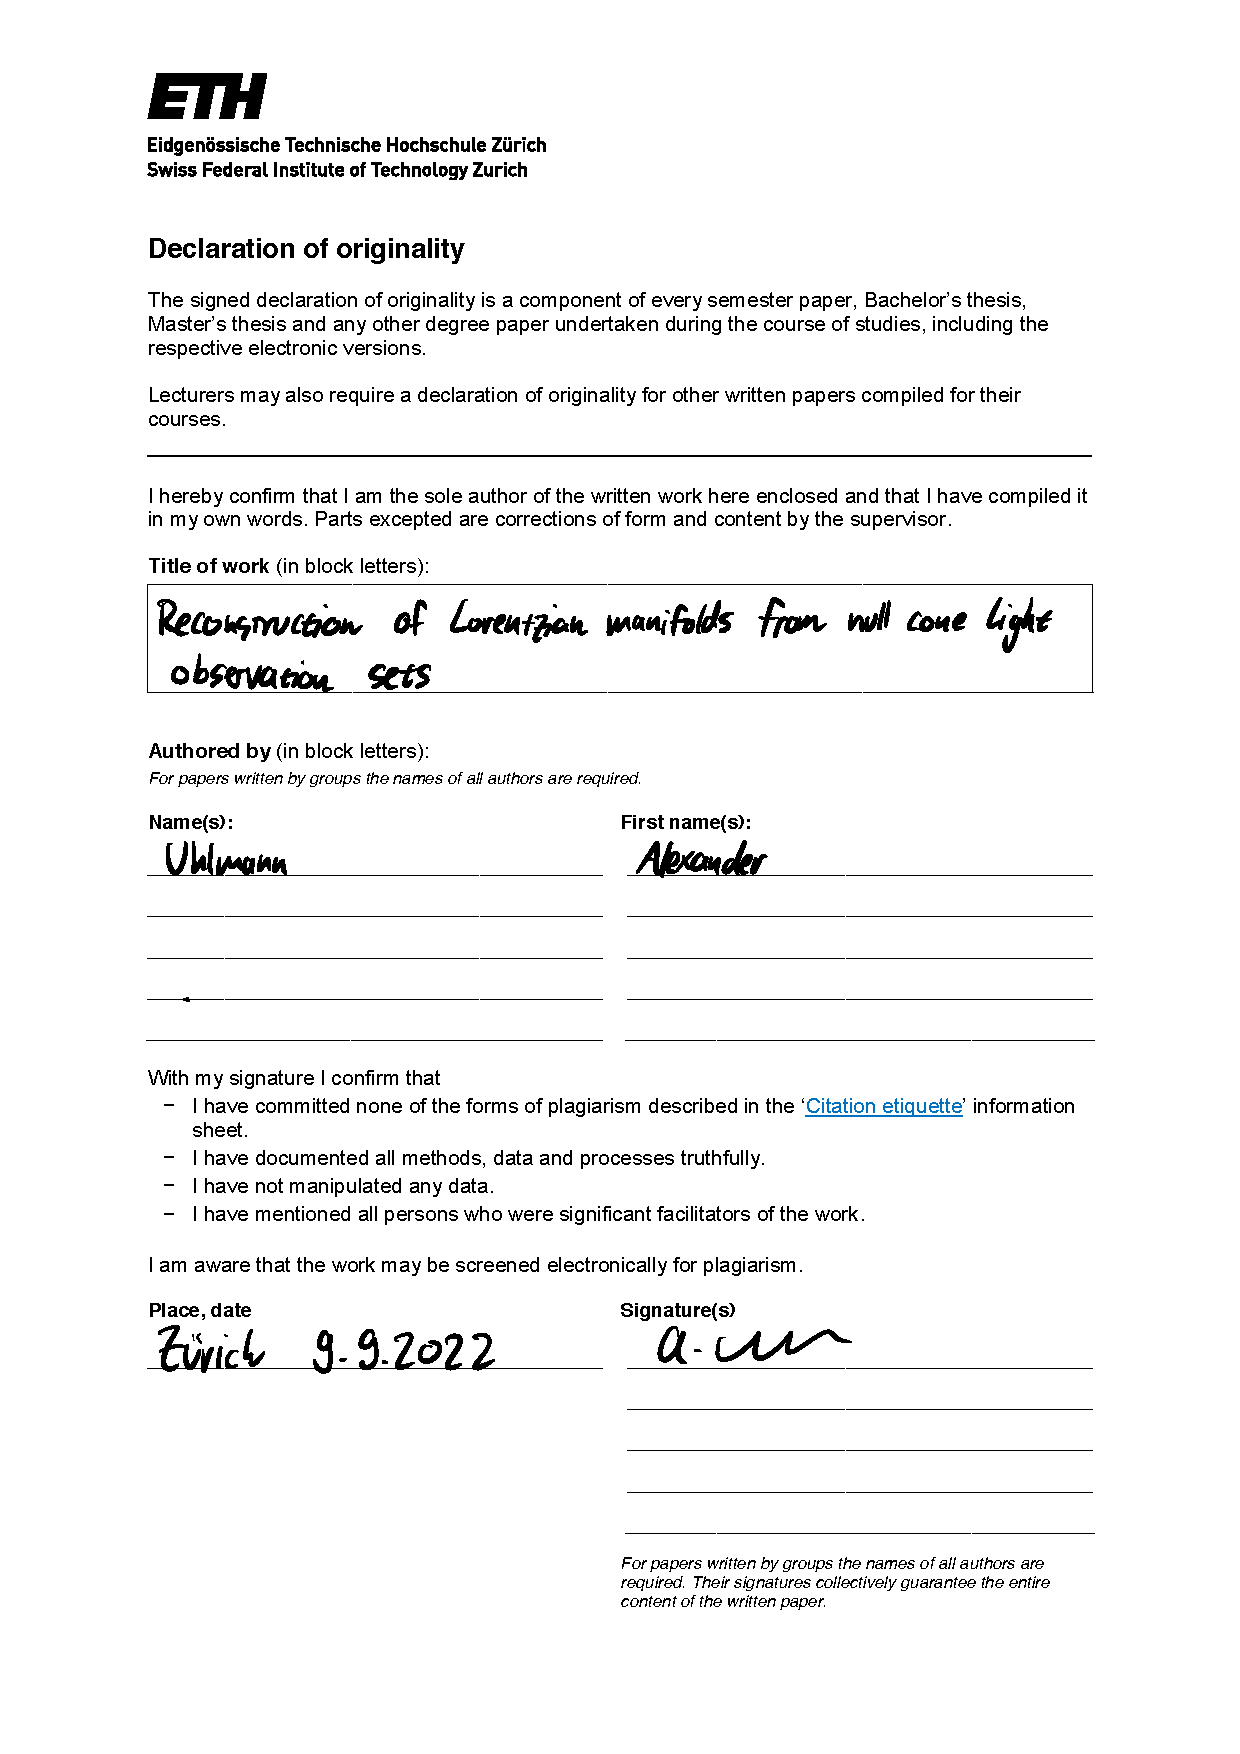
\includepdf[pages={-}]{declaration-originality.pdf}

\end{document}